%------------------------------%
%% ✎ Dylan (V1) %%%%%%%%% ✅ %%
%% ✎ Alain (V2) %%%%%%%%% ✅ %%
%% ✎ Dylan (V3) %%%%%%%%% ✅ %%
%------------------------------%

%%%%%%%%%%%%%%%%%%%%%%%%%%%%%%%%
% Chapter~1
\chapterheader{\textsl{Transit-Oriented Development} and Light Individual Mobility}
\chapter
{Challenges and Implications of \textsl{Transit-Oriented Development} Marked by the Rise of Light Individual Mobility
    \label{chap1:titre}
    }
    \begin{refsegment}

    % Background Chapter~1
    \AddToShipoutPictureBG*{%
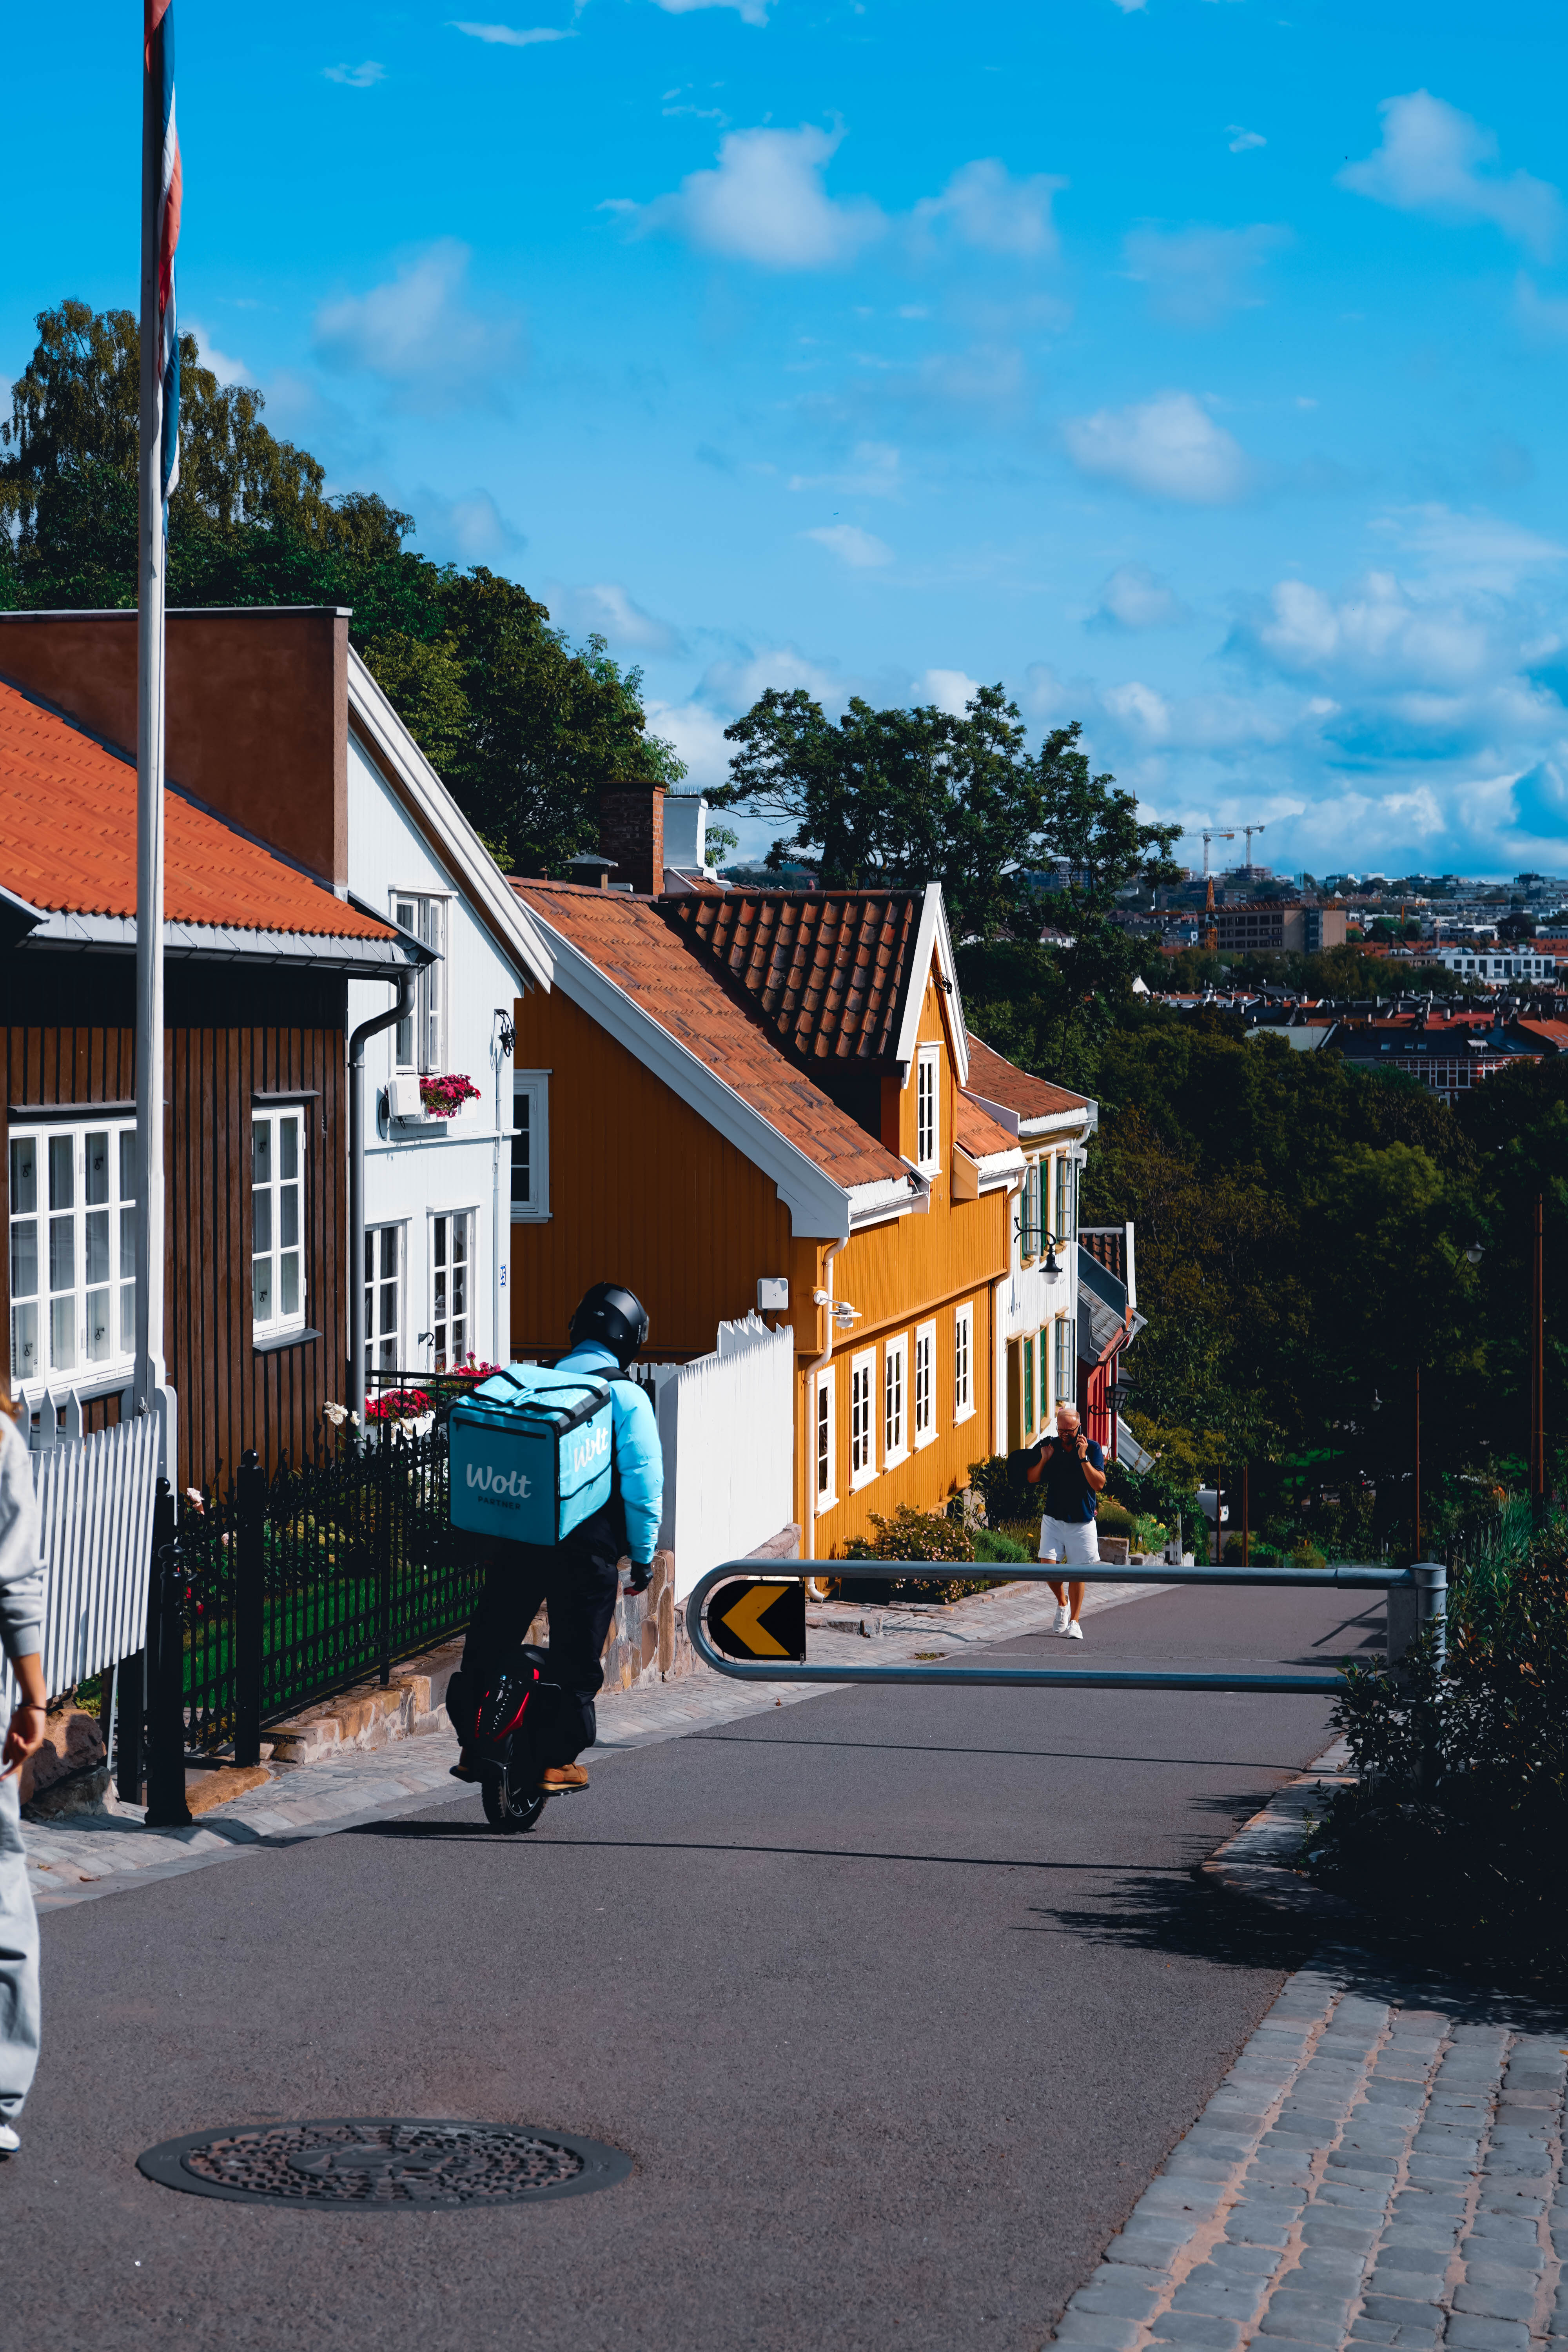
\includegraphics[width=\paperwidth,height=\paperheight]{src/Figures/Arriere_plan/Arriere_plan_Chap_1.jpg}
    }

% Rectangle
\AddToShipoutPictureBG*{
  \begin{tikzpicture}[remember picture,overlay]
    \node[fill=white, opacity=0.75, text width=\paperwidth, minimum height=11cm, anchor=north] 
    at ([yshift=-2cm]current page.north) {};
  \end{tikzpicture}
}

% Source
\AddToShipoutPictureFG*{
  \AtPageLowerRight{
    \raisebox{1cm}{
      \hspace{16cm}
      
\begin{tikzpicture}
        \node[fill=white, rounded corners=5pt, inner sep=5pt, align=center] {
          \tiny{Photography: \textcolor{blue}{Dylan Moinse (2023)}}
        };
      \end{tikzpicture}
    }
  }
}

    % ___________________________________________
    % Mini Table of Contents
    \cleardoublepage
    \setcounter{tocdepth}{2}
    % Redefine local table of contents title
    \renewcommand{\localcontentsname}{Table of Contents for Chapter~1}
\localtableofcontents

% Reset section numbering
\setcounter{section}{0}

    % ___________________________________________
    % Graphical Abstract
    \newpage
\section*{Key Points of Chapter~1
    \label{chap1:graphical-abstract}
    }
    \markright{Chapter Preamble}{}

\begin{figure}[h!]\vspace*{4pt}
        \caption*{Theoretical Framework of a \textsl{Micromobility-friendly Transit-Oriented Development}}
        \label{graphical-abstract-chap1}
        \centerline{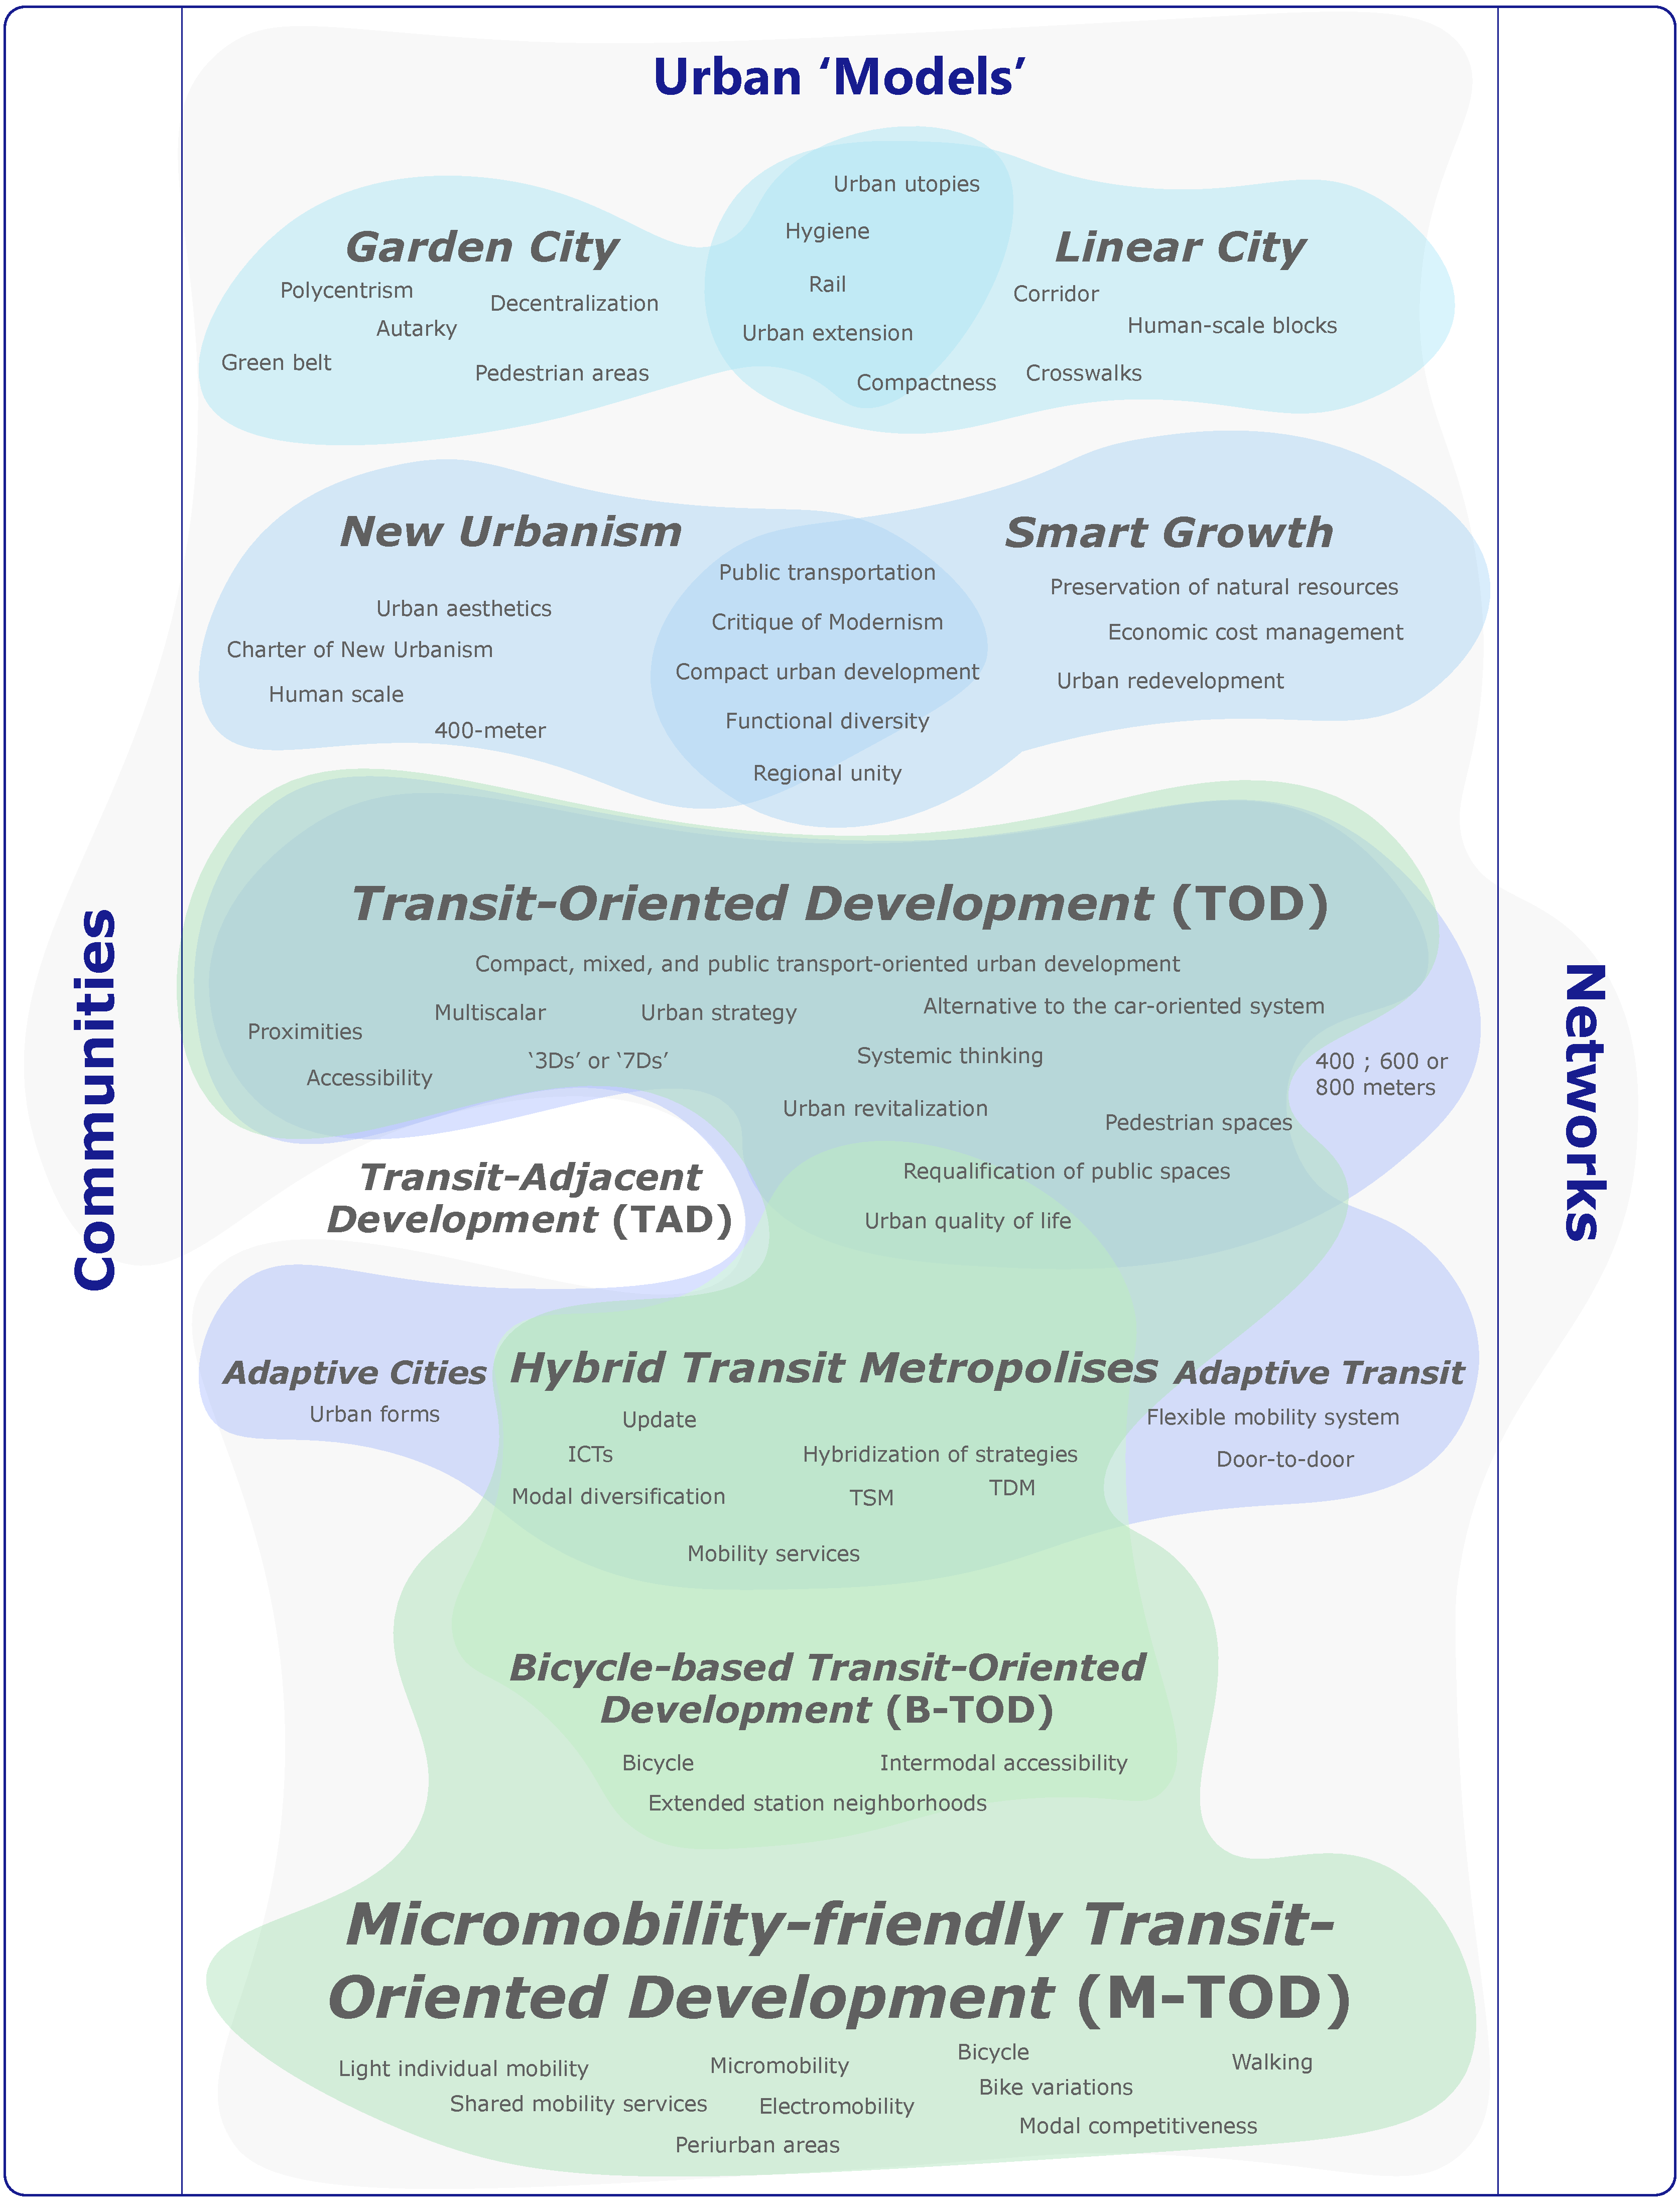
\includegraphics[width=1\columnwidth]{src/Figures/Graphical-abstract/EN_Graphical_abstract_chap1.pdf}}
        \vspace{5pt}
    \end{figure}
    
    % ___________________________________________
    % Preamble
    \newpage
    \begin{tcolorbox}[colback=white!5!white,
                      colframe=blue!75!blue,
                      title=
                      \bigskip
                      \center{\textbf{Preamble of Chapter~1}}
                      \\
                      \raggedright{\small{Chapter composed of \pagedifference{chap1:titre}{chap2:titre} pages, including \pagedifference{chap1:bibliographie}{chap2:titre} pages of bibliography}}
                      \bigskip]
\Large{\textbf{\textcolor{blue}{Abstract:}}}
    \\
    \small{
Formalized in the United States in the 1990s, \acrshort{TOD} represents an urban planning model based on the articulation between densification, functional diversity, public space requalification, and public transport development, with the objective of reducing automobile dependency and fostering a more resilient urban system. This concept follows a lineage of intellectual and urbanistic traditions inherited from several major historical currents. Among them, the \textsl{Garden City} and \textsl{Linear City} introduced planning structured around public transport infrastructures, while \textsl{New Urbanism} and \textsl{Smart Growth} updated these principles to address contemporary urbanization challenges and urban sprawl driven by automobile dominance. \textsl{TOD} thus materializes as an urban strategy aimed at structuring territorial organization \textsl{in connection} with the public transport network, promoting a compact, mixed-use city conducive to alternatives to private cars (see \hyperref[chap1:tod-presentation-generale]{Section~1}, page~\pageref{chap1:tod-presentation-generale}).%%Translated%%
    \\
However, implementing \acrshort{TOD} faces several challenges. While its principles remain particularly relevant for metropolitan areas with a dense and efficient rail network, their transposition to suburban territories encounters significant structural obstacles. The extension of travel distances, the fragmentation of locations, and the intrinsic limitations of public transport networks reduce the model’s effectiveness in such contexts. Furthermore, the rigidity of heavy infrastructures complicates their adaptation to inherited urban forms characterized by low density and high automobile dependence. In this perspective, the rise of light individual mobility—including bicycles, scooters, and other lightweight vehicles—offers a strategic lever to enhance accessibility to public transport stations and strengthen network connectivity. This development relies on a variety of technical, service-based, and social innovations, ranging from electromobility to the mutualization of shared fleets. Thus, integrating these modes could expand the reach of \acrshort{TOD} and maximize its benefits (see \hyperref[chap1:mobilite-individuelle-legere]{Section~2}, page~\pageref{chap1:mobilite-individuelle-legere}).%%Translated%%
    \\
This chapter explores, from a theoretical perspective, the potential of light individual mobility as a response to the limitations of \textsl{Transit-Oriented Development} (\acrshort{TOD}). By facilitating \Commas{first and last mile} travel, this category of alternative vehicles optimizes the use of public transport infrastructures while reducing dependence on private cars. Rather than replacing public transport, it follows a complementary intermodal logic, fostering a seamless integration within mobility systems. The evolution of travel practices and the rise of these (new) modes are transforming the relationship between public transport and urban planning, calling for a reinterpretation of established models. This is why we propose expanding the concept of \acrshort{TOD} into an updated urban model, which we refer to as \acrshort{M-TOD}, drawing inspiration from the principles of \acrshort{B-TOD} (see \hyperref[chap1:btod]{Section~3}, page~\pageref{chap1:btod}).%%Translated%%
    }
    \tcblower
\Large{\textcolor{blue}{\textbf{Keywords:}}}
    \\
    \small{
\textsl{Bicycle-based Transit-Oriented Development};
Electromobility;
Modal Hybridization;
\textsl{Hybrid Transit Metropolis};
Innovation;
Light Individual Mobility;
Shared Mobility;
\textsl{Transit-Oriented Development}
    }
    \end{tcolorbox}

% ___________________________________________
% 1.*.
\newpage
\needspace{1\baselineskip} % Reserve space
\addcontentsline{toc}{section}{Introduction of Chapter~1}
\sectionheader{Introduction of Chapter~1}
\section*{Introduction of Chapter~1
    \label{chap1:introduction}
    }
    \markright{Introduction of Chapter~1}{}

    % Citation
\begin{displayquote}
\Commas{\textsl{The} [\textsl{Transit-Oriented Development}] \textsl{model presented in this book} [\dots] \textsl{focus on transit and is meant to broden a larger movement~–~Neo-Traditional Planning and the New Urbanism~–~which has many dimensions and differing emphasis. These approaches share fundamental principles but set out in slightly different directions.} [\dots] \textsl{With regards to all these proposals, it is important to remember that there is no absolute template and that the specifics of place, economics, and politics will always color and balance the different directions.}}

\textcolor{blue}{Peter} \textcolor{blue}{\textcite[10-11]{calthorpe_next_1993}}\index{Calthorpe, Peter|pagebf}. \foreignlanguage{english}{\textsl{The Next American Metropolis: Ecology, Community, and the American Dream}}, Princeton Architectural Press, New York, 175~p. ISBN: \href{https://search.worldcat.org/fr/title/27814585}{1-878271-68-7}
    \end{displayquote}

% Introduction
\lettrine[lines=3, findent=8pt, nindent=0pt]{\lettrinefont F}{acing} the challenges of pollution, urban fragmentation, and congestion caused by the widespread use of automobiles and urbanization adapted to this mode of transportation, the concept of \acrfull{TOD} planning is based on the principle of densification and diversification of activities and uses around public \gls{public transport} infrastructure. Formalized in the United States under the impetus of \textcolor{blue}{Peter} \textcolor{blue}{\textcite[10]{calthorpe_next_1993}}\index{Calthorpe, Peter|pagebf}, this urban model draws from several schools of thought, notably the \textsl{Garden City} of \textcolor{blue}{Ebenezer} \textcolor{blue}{\textcite{howard_-morrow_1898}}\index{Howard, Ebenezer|pagebf}, the \textsl{Linear City} of \textcolor{blue}{Arturo Soria y Mata (1882)}, as well as the principles of \textsl{New Urbanism} and \textsl{Smart Growth}. A fundamental element of \acrshort{TOD} lies in its ability to explicitly articulate public transport and urban planning in a synergistic manner, far beyond a simple juxtaposition of infrastructure and activities. It is a multidimensional and multiscale approach where the public transport station becomes the structuring pivot of the territory. In this logic, the nodal point no longer merely connects flows but genuinely interacts with them by connecting to the place \textcolor{blue}{\autocite[344]{bertolini_nodes_1996}}\index{Bertolini, Luca|pagebf}, based on a \Commas{place-movement} approach \textcolor{blue}{\autocite[103]{le_bot_flux_2024}}\index{Le Bot, Nils|pagebf}. This model aims to promote a more compact and lively urbanism to better control urban sprawl and encourage travel by public transport, as well as on foot and by \gls{bicycle}. Moreover, it contributes to the reorganization of activities at the territorial scale by promoting a polycentric structure \textcolor{blue}{\autocite[38]{pearce_enquete_2020}}\index{Pearce, Marc|pagebf}\index{Landriève, Sylvie|pagebf}\index{Gay, Christophe|pagebf}\index{Dubois, Tom|pagebf}, in the manner of a \Commas{centralized decentralization} \textcolor{blue}{\autocite[55]{kamruzzaman_advance_2014}}\index{Kamruzzaman, Md.|pagebf}\index{Baker, Douglas|pagebf}\index{Washington, Simon|pagebf}\index{Turrell, Gavin|pagebf}. Today, \acrshort{TOD} is emerging as one of the urban strategies closest to what we can qualify as \Commas{sustainable urbanism} or \Commas{sustainable urban development} \textcolor{blue}{\autocite[14]{bentayou_transit-oriented_2015}}\index{Bentayou, Gilles|pagebf}. Furthermore, the latest report from the \acrfull{IPCC} recommends urban development oriented towards public transport networks and active modes, designed to promote urban compactness \textcolor{blue}{\autocite[29]{lee_climate_2023}}\index{Lee, Hoesung|pagebf}\index{Calvin, Katherine|pagebf}\index{Dasgupta, Dipak|pagebf}\index{Krinner, Gerhard|pagebf}\index{Mukherji, Aditi|pagebf}\index{Thorne, Peter|pagebf}\index{Trisos, Christopher|pagebf}\index{Romero, Jose|pagebf}\index{Aldunce, Paulina|pagebf}\index{Barrett, Ko|pagebf}\index{Blanco, Gabriel|pagebf}\index{Cheung, William|pagebf}\index{Connors, Sarah|pagebf}\index{Denton, Fatima|pagebf}\index{Diongue Niang, Aïda|pagebf}\index{Dodman, David|pagebf}\index{Garschagen, Matthias|pagebf}\index{Geden, Oliver|pagebf}\index{Hayward, Bronwyn|pagebf}\index{|pagebf}\index{Jones, Christopher|pagebf}\index{Frank, Jotzo|pagebf}\index{Thelma, Krug|pagebf}\index{Laco, Rodel|pagebf}\index{Lee, June-Yi|pagebf}\index{Masson-Delmotte, Valérie|pagebf}\index{Meinshausen, Malte|pagebf}\index{Mintenbeck, Katja|pagebf}\index{Mokssit, Abdalah|pagebf}\index{Otto, Friederike~E.~L.|pagebf}\index{Pathak, Minal|pagebf}\index{Pirani, Anna|pagebf}\index{Poloczanska, Elvira|pagebf}\index{Pörtner, Hans-Otto|pagebf}\index{Revi, Aromar|pagebf}\index{Roberts, Debra~C.|pagebf}\index{Roy, Joyashree|pagebf}\index{Ruane, Alex~C.|pagebf}\index{Skea, Jim|pagebf}\index{Shukla, Priyadarshi~R.|pagebf}\index{Slade, Raphael|pagebf}\index{Slangen, Aimée|pagebf}\index{Sokona, Youba|pagebf}\index{Sörensson, Anna~A.|pagebf}\index{Tignor, Melinda|pagebf}\index{Vuuren, Detlef~van.|pagebf}\index{Wei, Yi-Ming|pagebf}\index{Winkler, Harald|pagebf}\index{Zhai, Panmao|pagebf}\index{Zommers, Zinta|pagebf}.%%Translated%%

% Limites et intermodalité
However, the lengthening of distances and the fragmentation of production, consumption, and residential areas, resulting from functional zoning and the horizontal artificialization of soils, have significantly reduced the attractiveness and competitiveness of public transport across a large part of the territories \textcolor{blue}{\autocite[25-28]{mallet_voyage_2022}}\index{Mallet, Thierry|pagebf}. Moreover, the public transport system fails to match all the benefits provided by car use, particularly in terms of flexibility and connectivity \textcolor{blue}{\autocite[209]{heran_retour_2015}}\index{Héran, Frédéric|pagebf}. This situation thus questions the ability of the urban model to effectively address car dependency, especially in peri-urban areas. An alternative lies in promoting intermodality, which could mitigate the rigidity of the public transport network \textcolor{blue}{\autocite[17]{wiel_comment_1998}}\index{Wiel, Marc|pagebf} and improve the overall efficiency of the mobility system \textcolor{blue}{\autocite[82]{oostendorp_combining_2018}}\index{Oostendorp, Rebekka|pagebf}\index{Gebhardt, Laura|pagebf}. By moving beyond strictly monoscalar and monomodal approaches, corrective measures can be implemented to limit dysfunctions and optimize the performance of intermodal chains, from the regional to the intra-urban scale \textcolor{blue}{\autocite[111-115]{chapelon_transports_2016}}\index{Chapelon, Laurent|pagebf}. The goal is to design an integrated and coherent system where urban growth adapts to the development of public transport as much as alternative mobility solutions adjust to the specificities of the existing urban fabric. Empirically, this approach translates into adopting urban planning strategies that foster a dialogue between transport supply and demand, integrating complementary mobility solutions within a global rather than sectorized system. It is within this perspective that contemporary \textsl{Transit Metropolises} have developed, aiming to compete with the car by mimicking its \Commas{door-to-door} connectivity while adhering to a collective travel logic \textcolor{blue}{\autocite[132-133]{cervero_transit_2020}}\index{Cervero, Robert|pagebf}.%%Translated%%

% Mobilité individuelle légère
In this context, the rise of what we have chosen to call \Commas{light individual mobility}—including bicycles, scooters, and their various adaptations—opens new perspectives for sustainable urban planning and mobility. These solutions offer interesting alternatives to the challenges posed by the \Commas{first and last mile} of public transport and thus emerge as an essential missing link in the transition towards \Commas{ecomobile} mobility \textcolor{blue}{\autocites[4]{sebban_complementarite_2003}[25]{amar_homo_2016}{heran_transition_2018}}\index{Sebban, Annie-Claude|pagebf}\index{Motte, Alain|pagebf}\index{Héran, Frédéric|pagebf}\index{Amar, Georges|pagebf}. Light individual mobility is part of an \Commas{innovative rewriting of the past}, exemplified by the resurgence of bicycles in renewed forms and the rise of scooters as a utilitarian mode of transport \textcolor{blue}{\autocite[18]{amar_homo_2016}}\index{Amar, Georges|pagebf}. The development of these light modes as intermodal solutions reflects a renewal of proximity at various spatial scales \textcolor{blue}{\autocite{sadik-kahn_15-minute_2021}}\index{Sadik-Kahn, Janette|pagebf}, thereby enhancing the attractiveness of public transport and revealing an evolution in mobility values \textcolor{blue}{\autocite[110]{goletz_intermodality_2020}}\index{Goletz, Mirko|pagebf}\index{Haustein, Sonja|pagebf}\index{Wolking, Christina|pagebf}\index{L'Hostis, Alain|pagebf}. Ultimately, the ecomobile city, in contrast to the car-centric city model, relies on local circulation where the complementarity between bicycles and public transport constitutes one of the fundamental principles of a more integrated and resilient mobility system.%%Translated%%

% Annonce du plan 1
This chapter is organized into three main parts exploring the foundations, application, and evolution of \acrshort{TOD}. First, we will examine the origins and theoretical foundations of this urban model by tracing its historical and intellectual influences, as well as its evolution and applicability (\hyperref[chap1:tod-presentation-generale]{Section~1}, page~\pageref{chap1:tod-presentation-generale}). We will analyze the urban planning movements that shaped its formulation and codification before highlighting the unique aspects of \acrshort{TOD} (\hyperref[chap1:tod-presentation-generale-origines]{Subsection~1.1}, page~\pageref{chap1:tod-presentation-generale-origines}). This epistemological retrospective will allow us to precisely define its contours as an alternative urban development model to the car-centric paradigm, specifying its principles and expected benefits (\hyperref[chap1:tod-presentation-generale-definition]{Subsection~1.2}, page~\pageref{chap1:tod-presentation-generale-definition}). Finally, we will see how this planning concept has been interpreted within urban strategies deployed in the French context and its main variations related to our research subject (\hyperref[chap1:tod-presentation-generale-declinaisons]{Subsection~1.3}, page~\pageref{chap1:tod-presentation-generale-declinaisons}).%%Translated%%

% Annonce du plan 2
The second part will focus on the second object of study of this research, namely the family of vehicles grouped under the term \Commas{light individual mobility} (\hyperref[chap1:mobilite-individuelle-legere]{Section~2}, page~\pageref{chap1:mobilite-individuelle-legere}). We will trace the historical evolution of these technical and social objects—notably bicycles and scooters—by identifying and simplifying the reading of the major periods that marked their development, in order to better contextualize their current resurgence of interest (\hyperref[chap1:proximite-velo-trottinette]{Subsection~2.1}, page~\pageref{chap1:proximite-velo-trottinette}). We will then address the diversification of the uses and forms of these vehicles, characterized notably by their electrification and sharing in the \gls{public space}, thereby blurring the traditional boundaries between modes of transport (\hyperref[chap1:velo-micromobilite-innovations]{Subsection~2.2}, page~\pageref{chap1:velo-micromobilite-innovations}). This historical reflection will allow us to expose, in turn, the evolution of values attached to mobility and lifestyles, as well as the definitional challenges related to the scope of relevance of this family of vehicles (\hyperref[chap1:caracterisation-mobilite-individuelle-legere]{Subsection~2.3}, page~\pageref{chap1:caracterisation-mobilite-individuelle-legere}).%%Translated%%

% Annonce du plan 3
Lastly, the third part of this chapter will articulate the previous two by exploring the opportunities offered by the association between public transport and light individual mobility in a modal complementarity logic (\hyperref[chap1:btod]{Section~3}, page~\pageref{chap1:btod}). We will show that, although combined walking is not assimilated to light individual mobility, it remains the structuring element of \acrshort{TOD}. First, we will demonstrate how the real scope of combined walking tends to be underestimated and how light individual mobility can play a complementary role, fitting into a field of relevance that does not compete with walking but reinforces the \gls{accessibility} to public transport (\hyperref[chap1:btod-limites-tod]{Subsection~3.1}, page~\pageref{chap1:btod-limites-tod}). Finally, we will highlight the comparative advantages of such synergy and how this intermodal approach invites us to question the relevance of an expanded model, that of \acrfull{M-TOD} (\hyperref[chap1:btod-m-tod]{Subsection~3.2}, page~\pageref{chap1:btod-m-tod}).%%Translated%%

% ___________________________________________
% 1.1.
\newpage
\needspace{1\baselineskip} % Reserve space
\sectionheader{Concept of \textsl{Transit-Oriented Development}}
\section{Transit-Oriented Development: A Reinvention of Regional Planning Around Railways
    \label{chap1:tod-presentation-generale}
    }

% Introduction TOD
\acrshort{TOD} is now established as a key planning model in regional development, emphasizing rail infrastructure as the central axis of urban growth. This popular strategy is based on the idea of structuring territories around public transport nodes to reduce car dependency and promote more sustainable urbanization. Despite the urgency and importance of these issues, the underlying mechanisms influencing car use in urban environments remain insufficiently understood due to a still limited theoretical framework \textcolor{blue}{\autocite[1]{verbavatz_critical_2019}}\index{Verbavatz, Vincent|pagebf}\index{Barthelemy, Marc|pagebf}. The reflections of Italian architect and urban planner \textcolor{blue}{Alberto} \textcolor{blue}{\textcite[]{magnaghi_bioregion_2014}}\index{Magnaghi, Alberto|pagebf} provide an enriching contribution to this debate by introducing a bioterritorial approach, in which \Commas{urban bioregions} and networks become the pillars of integrated development that respects local ecosystems. However, \acrshort{TOD} stands out as one of the few planning concepts capable of directly addressing and tackling the \Commas{network urbanism} mindset \textcolor{blue}{\autocite[]{dupuy_urbanisme_1991}}\index{Dupuy, Gabriel|pagebf} in a globalized context, highlighting the complex interactions between mobility, urbanization, and sustainability \textcolor{blue}{\autocite[51]{el_hadeuf_ville_2017}}\index{El Hadeuf, Mounya|pagebf}\index{Laterrasse, Jean|pagebf}.%%Translated%%

% Annonce du plan
We will begin by introducing, through a diachronic approach, the origins of the urban model, highlighting the innovative aspects it brings to address contemporary challenges related to the necessary coordination between networks and territories (\hyperref[chap1:tod-presentation-generale-origines]{section on the inspirations of \textsl{Transit-Oriented Development}}, page~\pageref{chap1:tod-presentation-generale-origines}). This introduction will be followed by an overview of the general principles proposed by the planning model to address these issues, as well as the expected effects on territories and mobility behaviors (\hyperref[chap1:tod-presentation-generale-definition]{section on the directions of \textsl{Transit-Oriented Development}}, page~\pageref{chap1:tod-presentation-generale-definition}). Finally, we will pay particular attention to the evolving nature of this concept on a global scale, both in academic and operational settings. We will analyze the various adaptations that result from the specificities of each context and the advancement of knowledge. This reflection will lead us to consider the potential contribution of bicycles and \gls{micromobility} in a perspective of updating the \acrshort{TOD} (\hyperref[chap1:tod-presentation-generale-declinaisons]{section on the main variations of \textsl{Transit-Oriented Development}}, page~\pageref{chap1:tod-presentation-generale-declinaisons}).%%Translated%%

% 1.1.1. Chronologie TOD
\needspace{1\baselineskip} % Reserve space
\subsection{Genesis of \textsl{Transit-Oriented Development}: When Rail Inspires Urbanism
    \label{chap1:tod-presentation-generale-origines}
    }

% Introduction 1
Geography, like many related disciplines, has long emphasized the dynamic interaction between a place and its environment, conceptualizing the place as a \Commas{milieu} that generates activities and drives transformations. By moving beyond the simple notion of physical space, the territorial system acts both as a \textsl{stimulus} and a product of transformations \textcolor{blue}{\autocite[19-21]{hagerstrand_what_1970}}\index{Hägerstrand, Torsten|pagebf}. This approach includes the capacity of train stations, as liminal spaces, to act as catalysts for various developments \textcolor{blue}{\autocite[6]{baron_nouvelle_2024}}\index{Baron, Nacima|pagebf}\index{Le Bot, Nils|pagebf}\index{Detavernier, Pauline|pagebf}. In the 1970s, the \Commas{new geographers} focused their work on the study of networks \textcolor{blue}{\autocites{claval_nouveaux_1977}[166]{massardier_savants_1996}[112-113]{orain_geographie_2006}}\index{Massardier, Gilles|pagebf}\index{Claval, Paul|pagebf}\index{Orain, Olivier|pagebf}, leveraging the dense network of rail infrastructures to analyze reticular forms. These studies explored the reciprocal interactions between networks and territories at various geographical scales \textcolor{blue}{\autocite[6]{baron_nouvelle_2024}}\index{Baron, Nacima|pagebf}\index{Le Bot, Nils|pagebf}\index{Detavernier, Pauline|pagebf}.%%Translated%%

% Introduction 2
In this context, American architect and urban planner \textcolor{blue}{Peter} \textcolor{blue}{\textcite[10]{calthorpe_next_1993}}\index{Calthorpe, Peter|pagebf} proposed a planning model centered on public transport in his work \foreignlanguage{english}{\textsl{The Next American Metropolis: Ecology, Community, and the American Dream}}: the \acrfull{TOD}. This concept asserts itself as a multidimensional action strategy, primarily focused on the physical-spatial aspects of planning \textcolor{blue}{\autocite[10]{calthorpe_next_1993}}\index{Calthorpe, Peter|pagebf}, positing that changes in mobility behavior can stem from urban form. The major influences of \acrshort{TOD} are rooted in the broader framework of \textsl{New Urbanism} and \textsl{Smart Growth}, while introducing a new scale of analysis. Indeed, \textcolor{blue}{Robert} \textcolor{blue}{\textcite[7]{cervero_transit_1998}}\index{Cervero, Robert|pagebf} considers that \acrshort{TOD} shifts the traditional focus from neighborhood or community-level interventions to the connections between public transport and urbanization on a regional scale.%%Translated%%

% 1.1.1.1. Mouvements d'urbanisme
\needspace{1\baselineskip} % Reserve space
\subsubsection*{Legacy of Past Urban Reflections
    \label{chap1:tod-presentation-generale-origines-mouvements}
    }

% Introduction
In her seminal work \textsl{L’urbanisme, utopies et réalités: Une anthologie}, historian \textcolor{blue}{Françoise} \textcolor{blue}{\textcite{choay_urbanisme_1965}}\index{Choay, Françoise|pagebf} provides a framework for understanding the evolution of contemporary cities. According to the author's thesis, the science of urbanism as we know it today does not represent a novel solution to new problems but essentially consists of the reiteration and reproduction of discursive schemas inherited from the 19\textsuperscript{th} century, which she designates as \Commas{models}. This perspective allows us to question the historical and ideological foundations of \acrshort{TOD}. Since the planning concept is rooted in intellectual currents developed in the 1980s in response to the urbanization crisis in the United States and France \textcolor{blue}{\autocite[11]{lefebvre_droit_1967}}\index{Lefebvre, Henri|pagebf}, such as \textsl{New Urbanism} and \textsl{Smart Growth}. However, reducing its inspirations to these postmodern movements would be simplistic. The roots of this model extend to urban theories of the late 19\textsuperscript{th} century, notably the \textsl{Garden City}. \textcolor{blue}{Françoise} \textcolor{blue}{\textcite[259]{choay_urbanisme_1965}}\index{Choay, Françoise|pagebf} identifies the latter as a \Commas{culturalist urbanism}, stemming from a critical theoretical current of the industrial city and characterized by a nostalgic vision of an organic order\footnote{~
    In her typology of \Commas{pre-urbanism} and \Commas{urbanism} movements, \textcolor{blue}{Françoise} \textcolor{blue}{\textcite[277]{choay_urbanisme_1965}}\index{Choay, Françoise|pagebf} designates as \Commas{culturalists} the theoretical currents dating from the second half of the 19\textsuperscript{th} century that advocated for a circumscribed city based on an organic organization, in reaction to the progressive ideas of the time.
}.%%Translated%%

% Cité-jardin : théorie
The \acrshort{TOD} model draws heavily from the concept of the \textsl{Garden City}, originally developed by British urban planner \textcolor{blue}{Ebenezer} \textcolor{blue}{\textcite{howard_-morrow_1898}}\index{Howard, Ebenezer|pagebf}, in reaction to the chaotic urban growth accompanying industrialization in Europe, marked by a lack of urban planning. His thought, formalized in his pamphlet \textsl{Garden Cities of To-Morrow}, characterized by some observers as \Commas{urbaphobic} \textcolor{blue}{\autocite[7]{cavin_cites-jardins_2007}}\index{Cavin, Joëlle Salomon|pagebf}, is based on creating self-sufficient satellite towns on a human scale, embodying the \Commas{fantasy of the dreamed small town} \textcolor{blue}{\autocite[9]{fath_entre_2007}}\index{Fath, Sébastien|pagebf}, combining the advantages of urban and rural life. These towns were designed to be limited in size and extension, connected by rail networks, and organized in a polycentric system with green belts separating each urban center (see \hyperref[fig-chap1:schema-cite-jardin]{Figure~\ref{fig-chap1:schema-cite-jardin}}, page~\pageref{fig-chap1:schema-cite-jardin}). This social project (\textsl{Social City}) aimed to promote a hybrid urbanity oriented towards nature, in contrast to the industrial cities of its time. According to \textcolor{blue}{Robert} \textcolor{blue}{\textcite[38]{fishman_open_2011}}\index{Fishman, Robert|pagebf}, \acrshort{TOD} borrows from garden cities the notions of decentralization and polycentrism, as well as the design of pedestrian-friendly spaces served by railways.%%Translated%%

% Cité-jardin : exemples
Following the success of the first garden city, inaugurated in Letchworth in 1903 and designed by \textcolor{blue}{Ebenezer Howard} \textcolor{blue}{\autocite[9]{gaboriau_aux_2004}}\index{Gaboriau, Arnaud|pagebf}, its adoption in France was swift, with the construction of the first Cité Bruno in Dourges, Pas-de-Calais, between 1904 and 1908. This implementation of hygienist principles aimed to house the miners of the Compagnie des mines de Dourges. However, it was not until the interwar period that a significant number of garden cities flourished around major French cities. The original concepts were reinterpreted in these adaptations. Indeed, the French garden cities did not correspond to the autonomous towns envisioned by \textcolor{blue}{Ebenezer Howard}, which aimed to connect workplaces, shops, community facilities, and housing. Instead, they were more akin to residential zones, referred to as \Commas{banlieues-jardins}. This model thus underwent a specific appropriation that quickly discarded the economic aspect of self-sufficiency, while leading to numerous developments claiming this concept \textcolor{blue}{\autocite[238]{guelton_cite-jardin_2013}}\index{Gaboriau, Arnaud|pagebf}. An emblematic example of this adaptation is the cities developed by the Compagnie des chemins de fer du Nord, under the leadership of engineer \textcolor{blue}{Raoul Dautry}. Similar to the Cité de Lille-Délivrance, whose construction began in April 1921, two years after the establishment of a new marshaling yard in Lomme and the opening of a passenger station. This garden city is directly adjacent to the new station. Upon its inauguration in 1926, the Cité de cheminots de Lille-Délivrance comprised 835 dwellings and 3,228 inhabitants \textcolor{blue}{\autocite[19]{gaboriau_aux_2004}}\index{Gaboriau, Arnaud|pagebf}.%%Translated%%

% Figure Cité-jardin
\begin{carte}[h!]\vspace*{4pt}
    \caption{Schematic map of a network of six \Commas{satellite cities} with 32,000 inhabitants surrounding a \Commas{central city} with 58,000 inhabitants.}
    \label{fig-chap1:schema-cite-jardin}
    \centerline{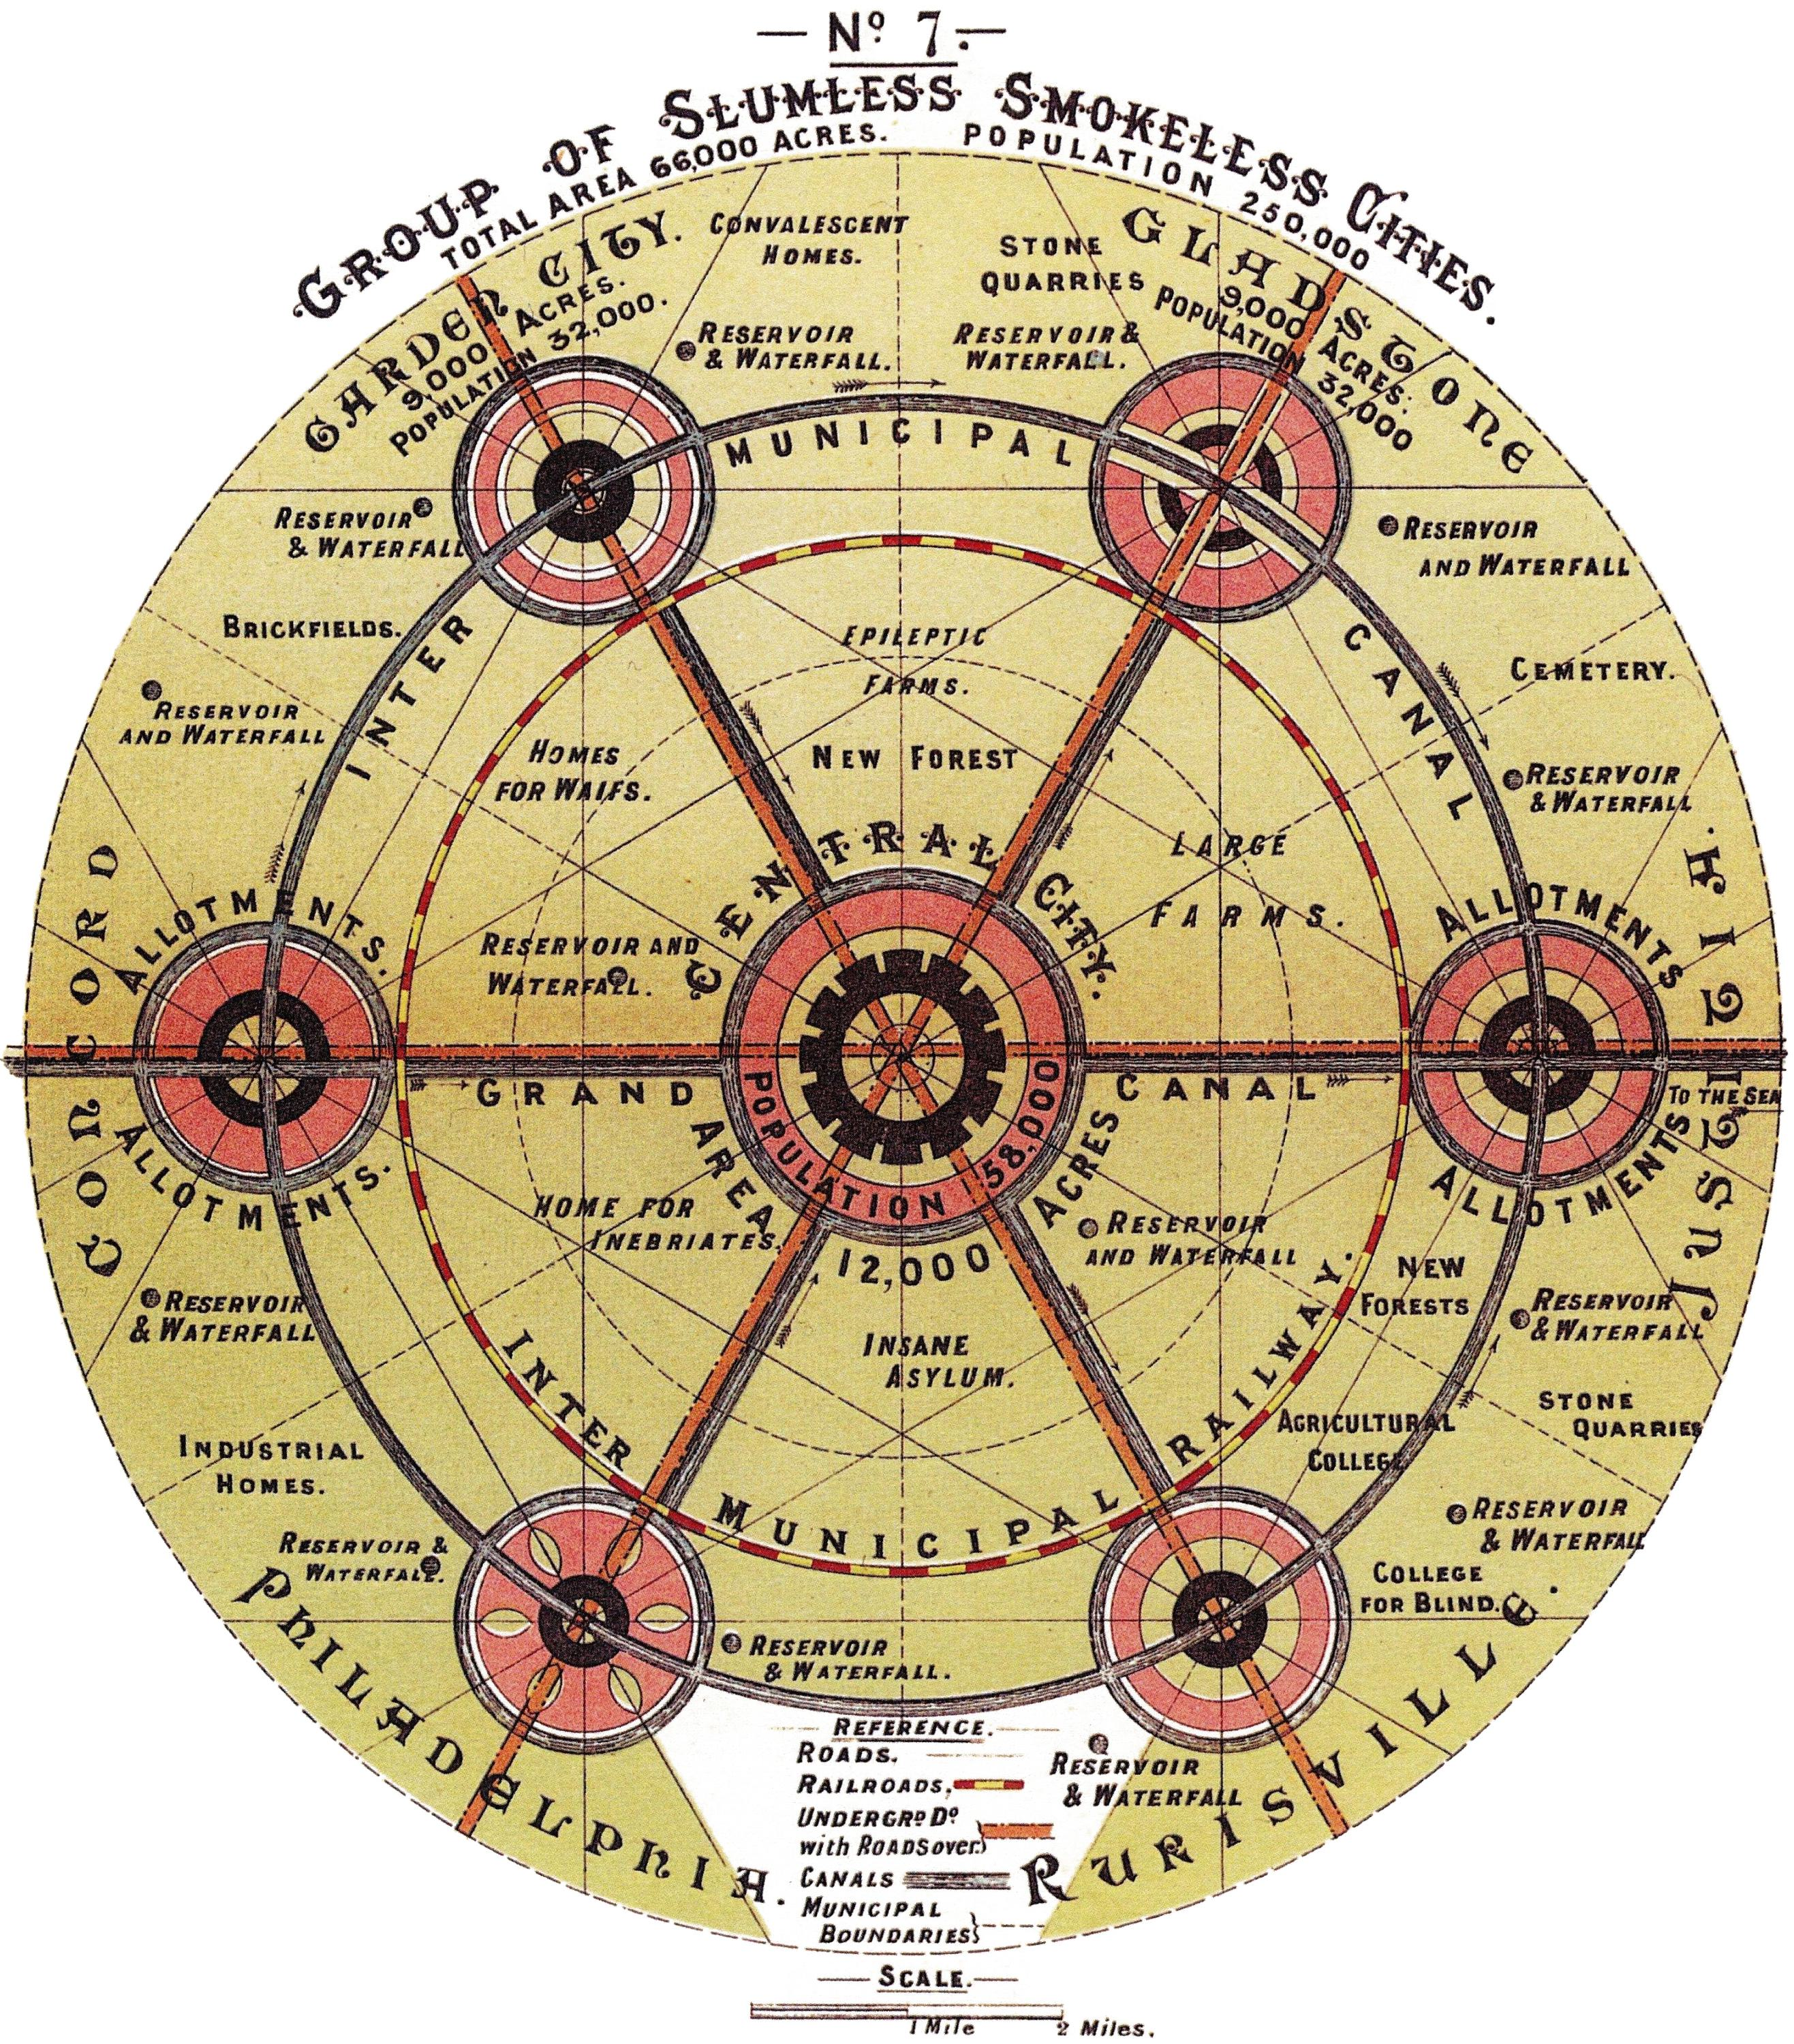
\includegraphics[width=0.75\columnwidth]{src/Figures/Chap-1/Cite_jardin.jpg}}
    \vspace{5pt}
    \begin{flushright}\scriptsize{
    Source: \textcolor{blue}{Ebenezer} \textcolor{blue}{\textcite[90]{howard_-morrow_1898}}\index{Howard, Ebenezer|pagebf}, cited by \textcolor{blue}{Stephen} \textcolor{blue}{\textcite[3]{ward_garden_1992}}\index{Ward, Stephen|pagebf}
    }\end{flushright}
\end{carte}

% Cité linéaire : théorie
Another utopian city concept that inspired \acrshort{TOD} is undoubtedly the \textsl{Linear City} (\textsl{Ciudad Lineal}), developed by \textcolor{blue}{Arturo Soria y Mata} in 1882 \textcolor{blue}{\autocite{lemelson_center_george_2014}}\index{Lemelson Center@\textsl{Lemelson Center}|pagebf}. By directing the urban expansion project over more than five kilometers along Madrid, the Spanish urban planner adopted a linear form to connect dense urban centers from the peripheries, an approach reminiscent of the corridor concept central to \acrshort{TOD} \textcolor{blue}{\autocite[348]{lopez_rodriguez_arturo_2017}}\index{López Rodríguez, Armando|pagebf}. The organization of the \textsl{Linear City} relies on a public transport mode, often the tramway, which becomes the backbone of the agglomeration \textcolor{blue}{\autocite{lemelson_center_george_2014}}\index{Lemelson Center@\textsl{Lemelson Center}|pagebf}. Unlike traditional urban growth, this urban utopia envisions a city without suburbs, capable of controlling its expansion along a corridor \textcolor{blue}{\autocite[722]{furundzic_infrastructure_2012}}\index{Furundzic, Danilo~S.|pagebf}\index{Furundzic, Bozidar~S.|pagebf}. Furthermore, the \Commas{matrix of this urban structure} is distinguished by privileged pedestrian accessibility, thanks to transverse promenades linking medium-density blocks. These two urban utopias—the \textsl{Garden City} and the \textsl{Linear City}—thus raise questions that remain relevant today and have significantly influenced \acrshort{TOD}, namely the promotion of a compact city designed both by and for public transport and walking \textcolor{blue}{\autocite[11]{salomon_cavin_cites-jardins_2007}}\index{Salomon Cavin, Joëlle|pagebf}.%%Translated%%

% Cité linéaire : exemples
The experimentation of this ideal city, initially envisioned to extend 53 kilometers around Madrid in a loop, ultimately saw only 5 kilometers realized, north-east of the Spanish capital, starting from 1894 \textcolor{blue}{\autocite[722]{furundzic_infrastructure_2012}}\index{Furundzic, Danilo~S.|pagebf}\index{Furundzic, Bozidar~S.|pagebf}. This project, designed by \textcolor{blue}{Arturo Soria y Mata}, planned radioconcentric connections linking this urban belt to the old city. In line with the hygienist city movement, this model exploited an axis encircling the existing city to facilitate the circulation of essential infrastructures such as railways, urban heating networks, electricity, or telephony. The horizontal organization of the linear city broke with the vertical structuring typical of the bourgeois city, while anticipating certain principles of the garden city, notably generalized access to individual property. More broadly, this concept evokes the notion of the \Commas{Urban Corridor} \textcolor{blue}{\autocite[63]{liu_corridors_2016}}\index{Liu, Liu|pagebf}\index{Menerault, Philippe|pagebf}\index{L'Hostis, Alain|pagebf}, allowing cities to expand linearly. In this regard, urban projects such as the \Commas{Grand Boulevard} connecting Lille, Roubaix, and Tourcoing can be seen as resonating with these principles. Inaugurated in 1909, this strategic artery, 14 kilometers long and 50 meters wide, features six circulation spaces dedicated respectively to automobiles, heavy horse-drawn transport, the Mongy tramway, riders, cyclists, and pedestrians who benefit from wide promenades\footnote{~
    Today, the Grand Boulevard is nonetheless perceived as a space more akin to an automobile transit area \textcolor{blue}{\autocite[139]{maitre_ambivalence_2016}}\index{Maitre, Elisa|pagebf}. Initially designed as an urban artery integrating two separate roadways, cycle paths, and sidewalks, this development has gradually evolved into an urban expressway, as successive connections have increased the traffic it supports. \textcolor{blue}{Philippe} \textcolor{blue}{\textcite[155]{menerault_gares_2008}}\index{Menerault, Philippe|pagebf} cites its integration with the A1 motorway, whose first section to Carvin was opened in 1954, and the A25 motorway towards Dunkirk in 1972.
} \textcolor{blue}{\autocite[87]{demangeon_lille-roubaix-tourcoing_1988}}\index{Demangeon, Alain|pagebf}\index{Werquin, Ann-Carol|pagebf}. Conceived as a structuring tool for urban growth, this project aimed to make the Grand Boulevard a regional showcase, nicknamed the \Commas{Champs-Élysées} of the metropolis, and to serve as the backbone of the future metropolis \textcolor{blue}{\autocite{dubuis__2020}}\index{Dubuis, Angélique Da Silva|pagebf}. The linear city has also inspired other interpretations and extensions, notably in Soviet experiments or through the reappropriation of this concept by \textcolor{blue}{Le Corbusier}. More recently, a notable example is the \textsl{The Line} project, announced by Saudi authorities as part of the Vision 2030 plan \textcolor{blue}{\autocite[139]{arnault_ville_2022}}\index{Arnault, Julie|pagebf}. Part of the new city project \textsl{Neom}, this concept, currently under construction, involves creating a linear city 170 kilometers long, 200 meters wide, and 500 meters high\footnote{~
    However, even before its concrete launch, the \textsl{The Line} project has been scaled back for 2030, with an infrastructure only 2.4 kilometers long instead of the initially planned 170 kilometers.
}. This infrastructure will be served by a high-speed train, theoretically allowing the entire city to be traversed in less than 20 minutes. Essential services will be distributed vertically, on each floor, and accessible in less than five minutes \textcolor{blue}{\autocite[139]{arnault_ville_2022}}\index{Arnault, Julie|pagebf}.%%Translated%%

% New Urbanism
From a more contemporary perspective, the roots of \acrshort{TOD} can be traced directly to \textsl{New Urbanism}, an urban planning and architectural movement that emerged in the 1980s in response to the limitations of modern urbanism \textcolor{blue}{\autocite[71]{liu_analyse_2016}}\index{Liu, Liu|pagebf}. This movement critiques the lack of functional and architectural diversity, the inadequate organization of public spaces, and the insufficient consideration given to pedestrians. Proposed as a rational alternative to the development of low-density, automobile-dominated suburban subdivisions, \textsl{New Urbanism} aims to rethink urban planning to make it more humane, aesthetically pleasing, and functional. Although inspired by certain principles of the modern movement, it distinguishes itself notably through the establishment, in 1989, of the \textsl{Congress for the New Urbanism}, often seen as the contemporary equivalent of the \acrfull{CIAM}. In 1996, this Congress ratified its own \textsl{Charter of the New Urbanism}\footnote{~
    This movement is not a monolithic bloc. It comprises two main complementary approaches \textcolor{blue}{\autocite[178]{ouellet_smart_2006}}\index{Ouellet, Michel|pagebf}. On one hand, the advocates of the \acrfull{TND} who emphasize a neotraditional aesthetic and urban organization, favoring compact neighborhoods with housing aligned along multi-intersection streets. On the other hand, the proponents of \acrshort{TOD} who prioritize the integration of public transport and more environmentally respectful regional urban planning. Although distinct, these two visions share a common objective: encouraging urban forms that promote functional mixity and reduce the ecological footprint of territories.
}. This \Commas{planning philosophy} advocates for compact urban development, planned on a human scale, that prioritizes public transport and the integration of diverse urban functions \textcolor{blue}{\autocite[177]{ouellet_smart_2006}}\index{Ouellet, Michel|pagebf}. From a practical standpoint, it recognizes several key characteristics of a neighborhood, including its optimal size, estimated at 400 meters from the center to the periphery \textcolor{blue}{\autocite[194]{ducharme_ville_2021}}\index{Ducharme, Olivier|pagebf}. Finally, \textsl{New Urbanism} adopts a regional perspective, considering the region as the basic territorial unit in a context of economic globalization \textcolor{blue}{\autocite[]{calthorpe_regional_2001}}\index{Calthorpe, Peter|pagebf}\index{Fulton, William|pagebf}. In this perspective, \acrshort{TOD} inherits the objective of promoting public transport to curb the artificialization of non-urbanized land \textcolor{blue}{\autocite[117]{lo_feudo_scenario_2014}}\index{Lo Feudo, Fausto|pagebf}\index{Menerault, Philippe|pagebf}\index{L'Hostis, Alain|pagebf}\index{Festa, Demetrio Carmine|pagebf}.%%Translated%%

% Smart Growth
The principles of \acrshort{TOD} also find their roots in a major contemporary urban planning movement: \textsl{Smart Growth}, which emerged in the late 1980s and became structured in the mid-1990s as an extension of the \Commas{sustainable urban development} paradigm \textcolor{blue}{\autocites[7]{bentayou_transit-oriented_2015}[71]{liu_analyse_2016}}\index{Bentayou, Gilles|pagebf}\index{Liu, Liu|pagebf}. This movement aims to preserve natural and financial resources while seeking to reduce spatial segregations, whether functional or social \textcolor{blue}{\autocite[7]{bentayou_transit-oriented_2015}}\index{Bentayou, Gilles|pagebf}. \textsl{Smart Growth} explicitly opposes uncontrolled urban sprawl by promoting more compact forms of development and urban redevelopment \textcolor{blue}{\autocites[176]{ouellet_smart_2006}{smart_growth_network_what_2015}}\index{Ouellet, Michel|pagebf}\index{Smart Growth Network@\textsl{Smart Growth Network}|pagebf}. These principles, shared by \textsl{New Urbanism}, value an integrated approach where transport and urban planning converge to create sustainable, socially equitable, and economically viable environments. \acrshort{TOD} is thus one of the tools enabling the realization of this \Commas{new} \Commas{smart} urbanism \textcolor{blue}{\autocite[7]{bentayou_transit-oriented_2015}}\index{Bentayou, Gilles|pagebf}.%%Translated%%

% Figure photographies Val d'Europe
\begin{figure}[h!]\vspace*{4pt}
    \caption{Photographs of the Val d'Europe sector, September 13, 2023.}
    \label{fig-chap1:photographies-val-europe}
    \centerline{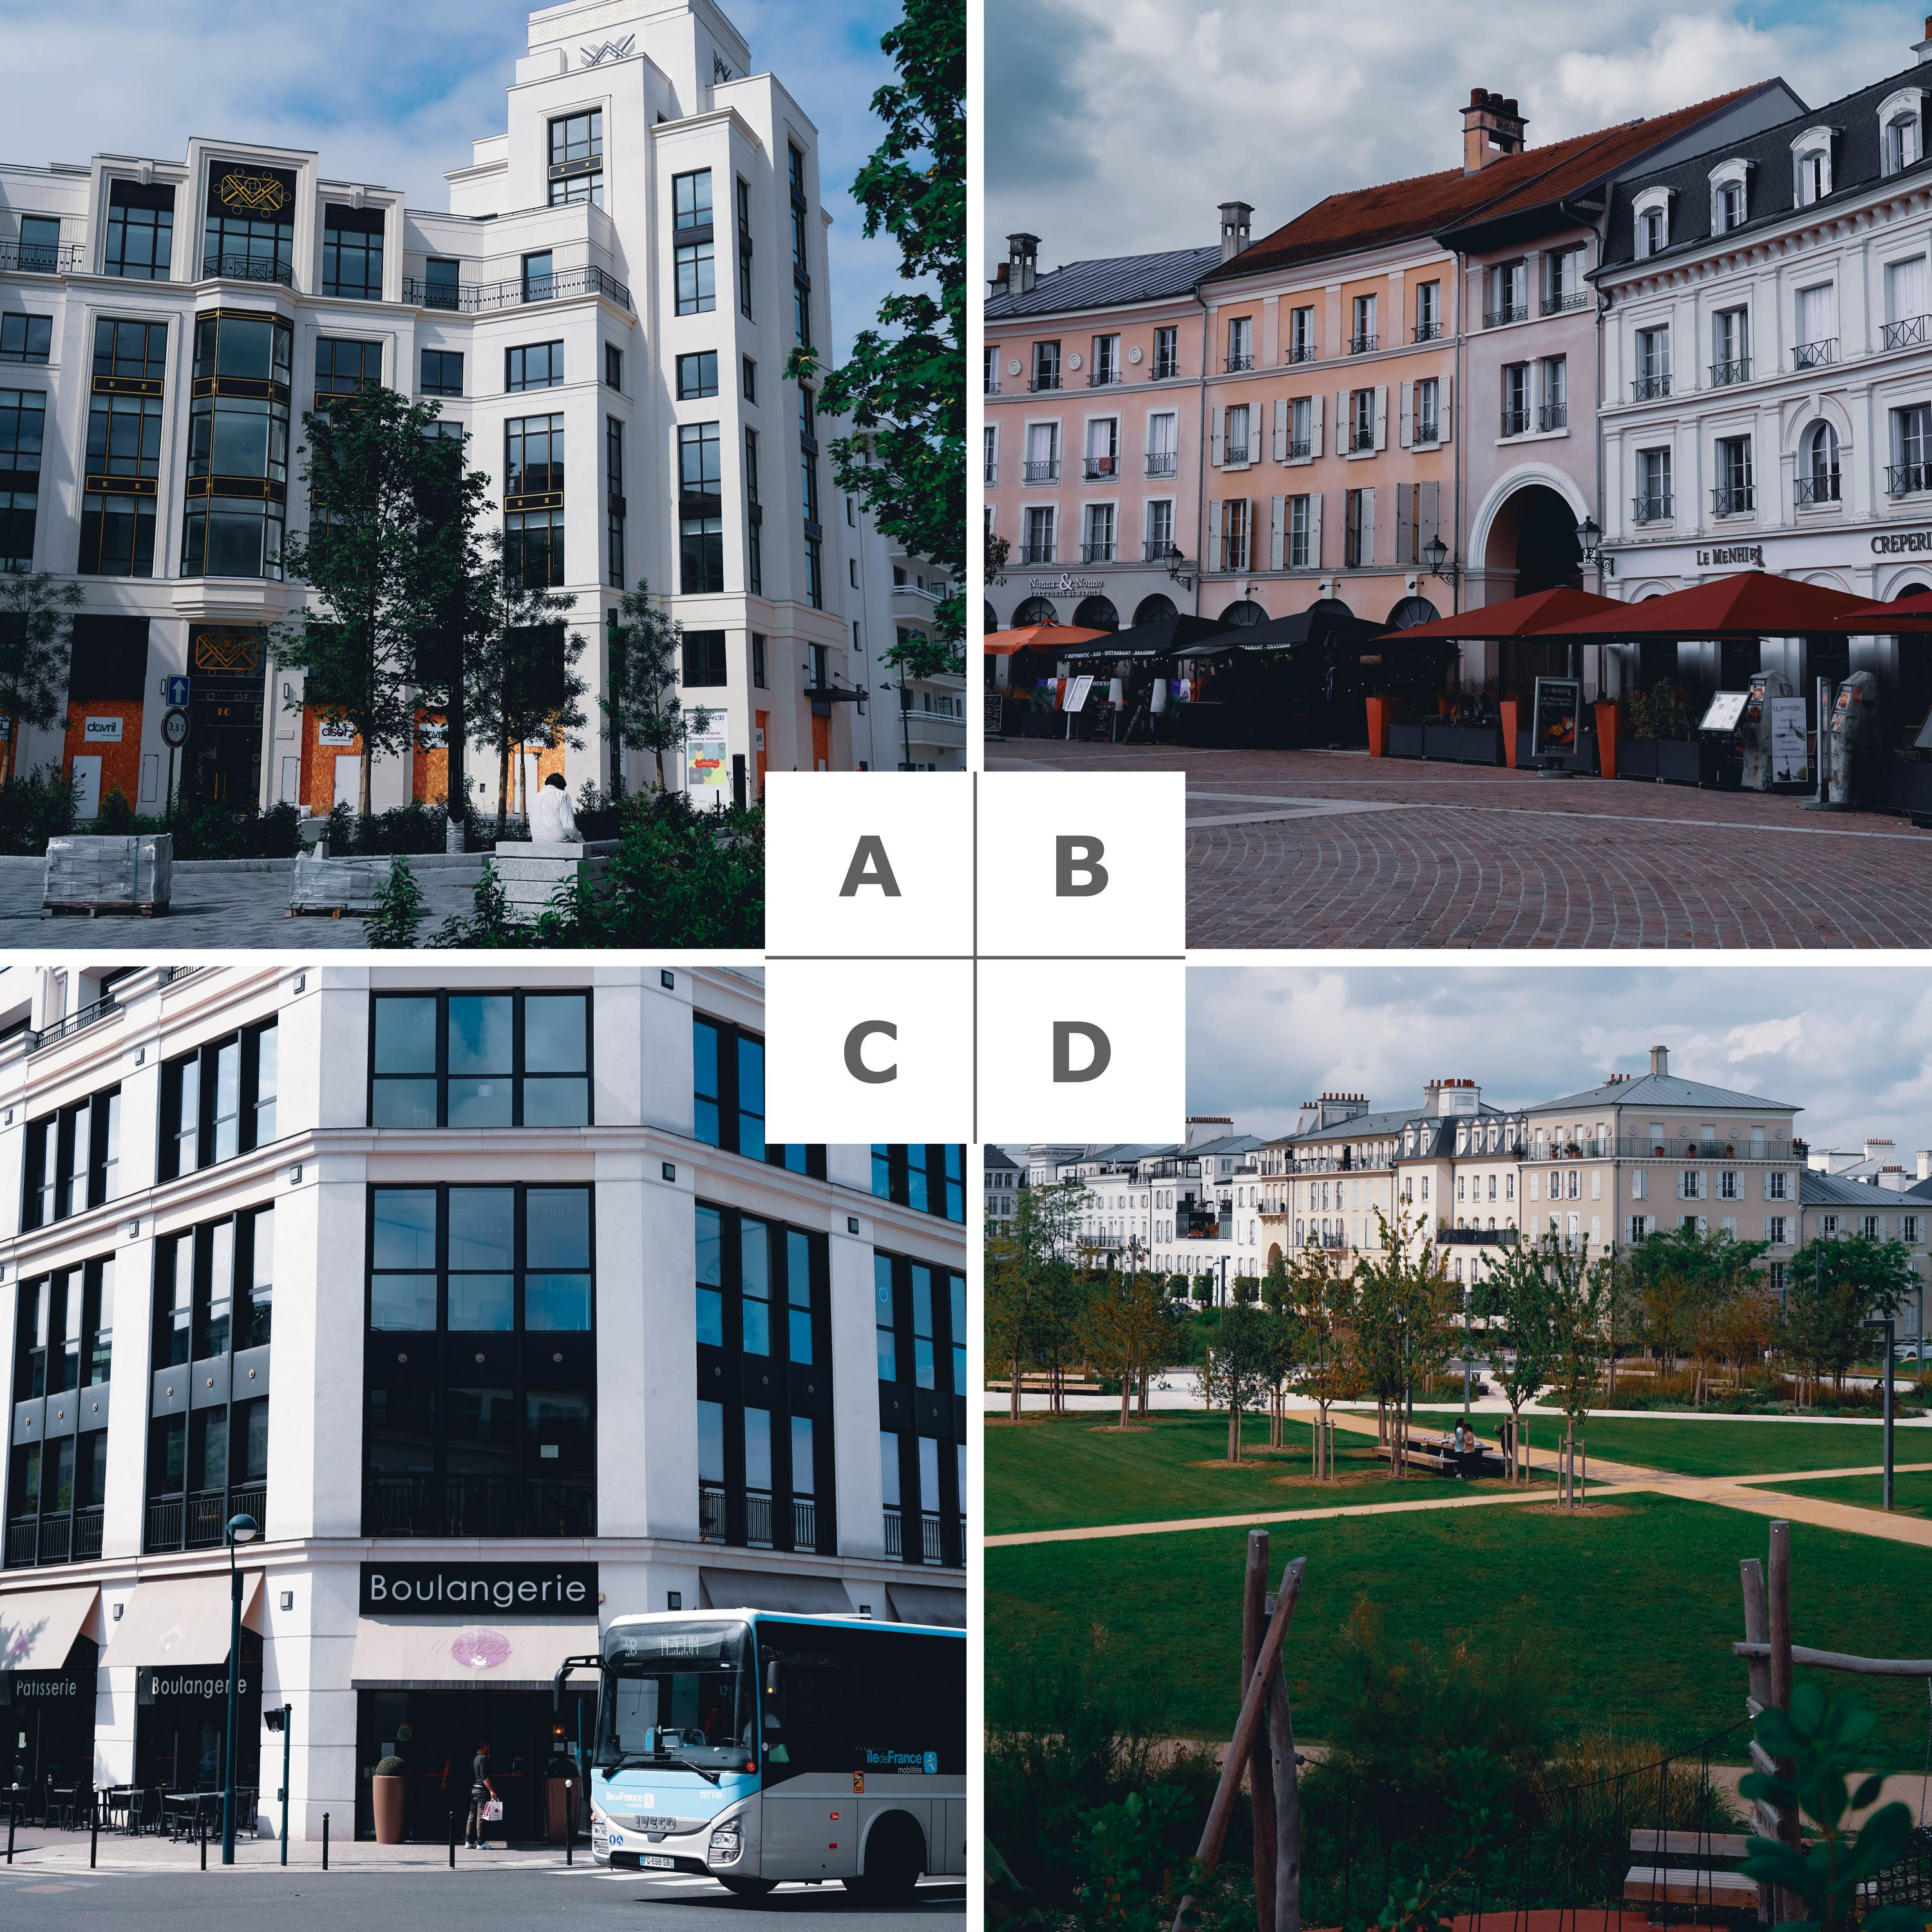
\includegraphics[width=0.75\columnwidth]{src/Figures/Chap-1/Val_Europe.jpg}}
    \vspace{5pt}
    \begin{flushright}\scriptsize{
    Photographies (A), (B), (C), and (D): \textcolor{blue}{Dylan Moinse (2023)}
  }\end{flushright}
\end{figure}

% Exemples New Urbanism/Smart Growth
Exemplary achievements illustrate the principles of \textsl{New Urbanism} and \textsl{Smart Growth}, such as the residential neighborhood of Laguna West in Sacramento, California, developed by \textcolor{blue}{Peter} \textcolor{blue}{\textcite[146-149]{calthorpe_next_1993}}\index{Calthorpe, Peter|pagebf}, a key figure in these movements. This is a \Commas{neotraditional} community, with the project launched in 1989 integrating 3,400 residential units, based on the pioneering concepts of American architect and urban planner \textcolor{blue}{Morris} \textcolor{blue}{\textcite[]{newman_focus_1991-1}}\index{Newman, Morris|pagebf}. Additionally, we examine the urban project Val d'Europe, the fourth sector of the new town of Marne-la-Vallée, awarded the \textsl{Charter Awards} in 2006 by the \textcolor{blue}{\textcite{congress_for_the_new_urbanism_cnu_2006}}\index{Congress for the New Urbanism@\textsl{Congress for the New Urbanism}|pagebf}. This urban project, developed along the A line of the \acrfull{RER} in the Paris region—the busiest line in Europe, inaugurated in 1969, although the Val d'Europe station opened in 2001—benefits from a strategic location near the Marne-la-Vallée—Chessy \acrshort{HST} station. It is a \acrfull{PPP} born from a collaboration between the French state and the \Marque{Walt Disney Company}, sealed by an agreement in 1987, aiming to develop and operate \Marque{Euro Disneyland} while integrating an urban center into the new town \textcolor{blue}{\autocite{epamarne_val_nodate}}\footnote{~
    The \acrfull{EPA} ÉpaMarne, in collaboration with ÉpaFrance, was tasked with overseeing Val d'Europe as part of a strategy to balance the territorial development of the Île-de-France region, traditionally dominated by the attractiveness of the \acrfull{CBD} of La Défense. This project embodies a dual ambition: creating an autonomous urban center on the outskirts of Paris and enhancing regional tourism appeal through the establishment of Disneyland Paris.
}. The planning of Val d'Europe is based on three principles aligned with the aforementioned movements: (i) an organization into neighborhoods, squares, and streets, favoring human scales; (ii) social and functional diversity, integrating housing\footnote{~
    The urban development of Val d'Europe continues. Adopted in 2016, the first \acrfull{PLUi} of the \acrshort{EPCI} plans the construction of 650 housing units per year, aiming for a total of 5,100 units, with 80\% being family homes. This plan also aims to meet the requirements of the \acrfull{SRU} regarding social housing, with 34\% of future housing being social housing, according to its \acrfull{PLH}.
}, commerce, and services\footnote{~
    For example, the Val d'Europe shopping center, opened in 2000, serves as the symbolic and functional heart of the city. It is divided into thematic zones and has been awarded for its design (\textsl{International Council of Shopping Centers Europe awards}).
}; and (iii) architecture inspired by European history, conferring an identity to each neighborhood (see \hyperref[fig-chap1:photographies-val-europe]{Figure~\ref{fig-chap1:photographies-val-europe}}, page~\pageref{fig-chap1:photographies-val-europe}). As \textcolor{blue}{\textcite[25]{dupuis_nouvelle_2017}}\index{Dupuis, Blaise|pagebf}\index{Söderström, Ola|pagebf} explain, Val d'Europe, as a \Commas{new traditional town}, embodies the principles advocated\footnote{~
    However, the development of Val d'Europe raises questions about its governance model and urban design. The involvement of a private operator in urban management has imposed a commercial vision of urban development. This approach has often been criticized for its tendency towards \Commas{Disneyfication} or \Commas{museification} of urban space \textcolor{blue}{\autocite[]{brunel_planete_2012}}\index{Brunel, Sylvie|pagebf}. These notions refer to an idealized and hyper-controlled model, characterized by a fictional and standardized reproduction of urban landscapes and histories, designed to meet the stereotypical expectations of tourists \textcolor{blue}{\autocite[7]{claude_developpement_2021}}\index{Claude, Appolline|pagebf}\index{Laage de Meux, Olivia de|pagebf}\index{Delpuech, Inès|pagebf}\index{Dextreit, Natalia|pagebf}\index{Poquillon, Mathilde|pagebf}\index{Praderie, Mila|pagebf}. Critics also highlight the risks of disconnection between this idealized city and social and economic realities. They question the balance between entrepreneurial imperatives, social inclusion, and sustainability. Furthermore, the negotiation processes between public and private actors have been marked by tensions, revealing the limits of a \acrshort{PPP} in such urban projects. An example is the location of the regional shopping center Val d'Europe. The private operator, likely influenced by a \Commas{culture of indifference towards public transport} \textcolor{blue}{\autocite[656]{tan_identifying_2014}}\index{Tan, Wendy|pagebf}\index{Bertolini, Luca|pagebf}\index{Janssen-Jansen, Leonie|pagebf}, wanted to locate this facility on the outskirts of the highway, far from the transit hub and the \acrshort{RER} station.
}, namely urban compactness, neighborhood organization, and aesthetic and morphological principles rooted in the heritage of past centuries \textcolor{blue}{\autocite[12]{moinse_exploring_2023}}\index{Moinse, Dylan|pagebf}.%%Translated%%

% Transition
The concept of \acrshort{TOD}, centered on compact, mixed, and transit-oriented urban development, draws from a lineage of urban planning movements that preceded it. These influences are fully acknowledged by \textcolor{blue}{Peter Calthorpe}, one of the main theorists of \acrshort{TOD}, who defines himself as a \Commas{restorer rather than an originator of ideas}\footnote{~
    \Commas{\textsl{Mr. Calthorpe, who calls himself a reviver rather than an originator of ideas} [\dots]} \textcolor{blue}{\autocite[5]{newman_focus_1991}}\index{Newman, Morris|pagebf}.
} \textcolor{blue}{\autocite[5]{newman_focus_1991}}\index{Newman, Morris|pagebf}. While the precursors of \acrshort{TOD} can be identified in models such as the \textsl{Garden City} or the \textsl{Linear City}, or in major figures of urban planning history like \textcolor{blue}{Ildefons Cerdà} or \textcolor{blue}{Georges-Eugène Haussmann}, these examples illustrate the evolution of ideas in urban planning. In the garden city, for instance, the train station plays a limited functional role, merely connecting self-sufficient cities to each other and their environment. \textcolor{blue}{Peter} \textcolor{blue}{\textcite[43-49]{calthorpe_next_1993}}\index{Calthorpe, Peter|pagebf}, on the other hand, reverses this principle: in \acrshort{TOD}, the transit station becomes the structuring center of urban development, moving beyond the logic of self-sufficiency to create connections within a fragmented and dispersed contemporary city \textcolor{blue}{\autocite[51]{el_hadeuf_ville_2017}}\index{El Hadeuf, Mounya|pagebf}\index{Laterrasse, Jean|pagebf}. This distinction marks a conceptual turning point. Unlike \textsl{New Urbanism} and \textsl{Smart Growth}, which primarily oppose uncontrolled urban sprawl, \acrshort{TOD} asserts a leading role for transport infrastructure in structuring the city \textcolor{blue}{\autocite[51]{el_hadeuf_ville_2017}}\index{El Hadeuf, Mounya|pagebf}\index{Laterrasse, Jean|pagebf}. Where \textsl{New Urbanism} promotes human-scale density and aesthetics, and \textsl{Smart Growth} prioritizes the preservation of natural resources and functional diversity, \acrshort{TOD} distinguishes itself by its ambition to reconnect dispersed territories through a transport-centered organization. Although most morphological components—such as the presence of a station, density, and compactness—are similar, this approach reflects a shift in scale between the 19\textsuperscript{th}-century city, still conceived as a coherent whole, and the contemporary city, which requires tools to restore its cohesion \textcolor{blue}{\autocite[37]{leysens_reconfiguration_2011}}\index{Leysens, Thomas|pagebf}\index{Menerault, Philippe|pagebf}\index{L'Hostis, Alain|pagebf}.%%Translated%%

% 1.1.1.2. TOD aspects contemporains
\needspace{1\baselineskip} % Reserve space
\subsubsection*{Originality and Reinterpretation of Planning Around Rail
    \label{chap1:tod-presentation-generale-origines-originalite}
    }

% Introduction
The movement that gave rise to \acrshort{TOD} is part of an intellectual and urban planning lineage shared by several critical and activist currents, united in their opposition to the car-centric city paradigm\footnote{~
    Since the 1960s, and even post-war, the dominance of the automobile in urban spaces began to be questioned, sparking growing criticism of its mass use and implications for urban planning \textcolor{blue}{\autocites{jacobs_death_1961}{illich_energie_1973}}\index{Jacobs, Jane|pagebf}\index{Illich, Ivan|pagebf}\index{Giard, Luce|pagebf}\index{Bardet, Vincent|pagebf}. This transition to the \Commas{third age of the city} \textcolor{blue}{\autocite[4]{newman_land_1996}}\index{Newman, Peter W.~G.|pagebf}\index{Kenworthy, Jeffrey~R.|pagebf}, marked by the \Commas{culture of the automobile} \textcolor{blue}{\autocite[157]{urry_social_2003}}\index{Urry, John|pagebf}, still structures most territories today, with direct and indirect consequences for planning, mobility behaviors, and lifestyles \textcolor{blue}{\autocite[40]{sebban_complementarite_2003}}\index{Sebban, Annie-Claude|pagebf}\index{Motte, Alain|pagebf}.
}. \textcolor{blue}{\autocites{jacobs_death_1961}{illich_energie_1973}}\index{Jacobs, Jane|pagebf}\index{Illich, Ivan|pagebf}\index{Giard, Luce|pagebf}\index{Bardet, Vincent|pagebf}, and particularly the numerous negative externalities associated with this model\footnote{~
    The negative externalities generated by automobile dependence include internal nuisances such as urban congestion, which compromises the economic and residential attractiveness of territories, as well as broader external effects: road accidents, urban fragmentation, socio-spatial exclusion, increased consumption of agricultural and natural spaces, loss of biodiversity, multiple pollutions (air, water, soil, noise, and visual), and degradation of quality of life, ranging from physical and mental health issues to chronic stress and reduced productivity. These externalities contribute to what some authors refer to as the \Commas{spiral of automobile dependence} or \Commas{cycle of auto-dependence}, where the automobile creates problems that only its intensified use seems able to solve \textcolor{blue}{\autocites[62]{cervero_transit_1998}[4]{heran_reduction_2001}[2]{heran_zones_2009}}\index{Cervero, Robert|pagebf}\index{Héran, Frédéric|pagebf}\index{Pouillaude, Laurence|pagebf}.
}. \textcolor{blue}{\autocites[62]{cervero_transit_1998}[4]{heran_reduction_2001}[2]{heran_zones_2009}}\index{Cervero, Robert|pagebf}\index{Héran, Frédéric|pagebf}\index{Pouillaude, Laurence|pagebf}. The \Commas{automobile system}, characterized by an organizational mode centered on technical performance and apparent advantages of the car, constitutes a captive and rigid structure\footnote{~
    Automobile dependence, along with \Commas{automobility}—denoting a way of life and associated representations—is based on cultural, socio-economic, urban planning, and technocratic factors \textcolor{blue}{\autocite[12]{heran_reduction_2001}}\index{Héran, Frédéric|pagebf}. The \Commas{all-automobile} is the product of aspirations linked to individual home and garden ownership, elevated living standards combined with consumption norms, urban forms favoring motorized travel, and the continuous improvement of car performance relative to other modes of transport.
}. The \Commas{hidden costs} associated with this system, i.e., the costs not covered by the community, are estimated at approximately 3\% of the annual \acrfull{GDP} of the \acrfull{EU}, revealing its collective inefficiency \textcolor{blue}{\autocite[34]{becker_couts_2012}}\index{Becker, Udo~J.|pagebf}\index{Becker, Thilo|pagebf}\index{Gerlach, Julia|pagebf} and its contribution to a genuine \Commas{tragedy of the commons} \textcolor{blue}{\autocite{hardin_tragecommuns_1968}}\index{Hardin, Garrett|pagebf}, where intensive use of road spaces by certain individuals leads to detrimental consequences for society as a whole \textcolor{blue}{\autocite[23]{6t-bureau_de_recherche_livre_2019}}\index{Bureau de recherche 6t@\textsl{Bureau de recherche 6t}|pagebf}. It should be noted that these estimates remain underestimated, particularly due to the lack of systematic consideration of complex feedback loops affecting climate change and public health \textcolor{blue}{\autocite[66, 72]{gossling_social_2019}}\index{Gössling, Stephan|pagebf}\index{Choi, Andy|pagebf}\index{Dekker, Kaely|pagebf}\index{Metzler, Daniel|pagebf}. It is precisely in this critical context that the \acrshort{TOD} concept is deployed as a multidimensional response aimed at addressing the dysfunctions of the car-centric model.%%Translated%%

% Lutte contre la dépendance automobile
Indeed, more than an invention \textsl{ex nihilo}, \acrshort{TOD} primarily constitutes an adaptation to a renewed urban context, characterized by the complexity and \Commas{speed} of modern cities. It offers an articulated alternative to the widespread diffusion and use of the automobile by introducing principles, perspectives, and operational tools to address current challenges at various spatial scales \textcolor{blue}{\autocite[37]{leysens_reconfiguration_2011}}\index{Leysens, Thomas|pagebf}. This is where the original contributions of the model lie \textcolor{blue}{\autocite[121]{lo_feudo_scenario_2014}}\index{Lo Feudo, Fausto|pagebf}\index{Menerault, Philippe|pagebf}\index{L'Hostis, Alain|pagebf}\index{Festa, Demetrio Carmine|pagebf}: the idea that the automobile should no longer be the benchmark for urban space planning must be abandoned \textcolor{blue}{\autocite[190]{ducharme_ville_2021}}\index{Ducharme, Olivier|pagebf}. \textcolor{blue}{Peter} \textcolor{blue}{\textcite{calthorpe_next_1993}}\index{Calthorpe, Peter|pagebf} thus essentially formalized the close relationship between urban development and public transport, establishing it as a structuring principle of \acrshort{TOD}. In this framework, \acrshort{TOD} defines the bases of a \Commas{new American dream}: unlike preceding currents primarily focused on aesthetic or social concerns, \acrshort{TOD} favors a resolutely regional approach. It is no longer merely a collection of dispersed urban projects within a contemporary city \textcolor{blue}{\autocite[357]{mongin_ville_2013}}\index{Mongin, Olivier|pagebf}. It integrates the imperative of reducing automobile use at the very core of urban planning functions \textcolor{blue}{\autocite[11]{calthorpe_next_1993}}\index{Calthorpe, Peter|pagebf}.%%Translated%%

% Oriented
The second innovation brought by \acrshort{TOD} lies in its ability to adjust to the context of growing automobile use while proposing a collective reflection nourished by international experiences. It notably introduces a third structuring element in the relationship between \textsl{transit} and \textsl{development}: the idea of orientation (\textsl{oriented}). In this regard, this form of connection is decisive, as noted by \textcolor{blue}{Fausto} \textcolor{blue}{\textcite[116]{lo_feudo_scenario_2014}}\index{Lo Feudo, Fausto|pagebf}. This notion goes beyond mere geographical proximity to embrace a global and coherent organization of intervention zones. Consequently, the scientific community that contributed to the evolution of the \acrshort{TOD} model advocates a holistic vision of urbanism \textsl{oriented} towards public transport, making public spaces a pivot in the articulation between the network and urban development. Thus, \acrshort{TOD} is not limited to a series of isolated operations near a station \textcolor{blue}{\autocite[124]{lhostis_ville_2013}}\index{L'Hostis, Alain|pagebf}\index{Soulas, Claude|pagebf}\index{Wulfhorst, Gebhard|pagebf}\index{Brun, Gérard|pagebf}. It is part of a broader strategic logic of redistribution along the corridors of the public transport network, considering the regional spatial structure and valorizing a \Commas{trace-based, connecting, and mixed urbanism}, in contrast to the \Commas{sector-based, secure, and homogeneous urbanism} that prevails \textcolor{blue}{\autocite[4-6]{mangin_ville_2004}}\index{Mangin, David|pagebf}.%%Translated%%

% Figure Murdoch
\begin{figure}[h!]\vspace*{4pt}
    \caption{Aerial view (A) and first-person view (B) of the surroundings of Murdoch station, connected to the Transperth network, in Australia.}
    \label{fig-chap1:tad-murdoch}
    \centerline{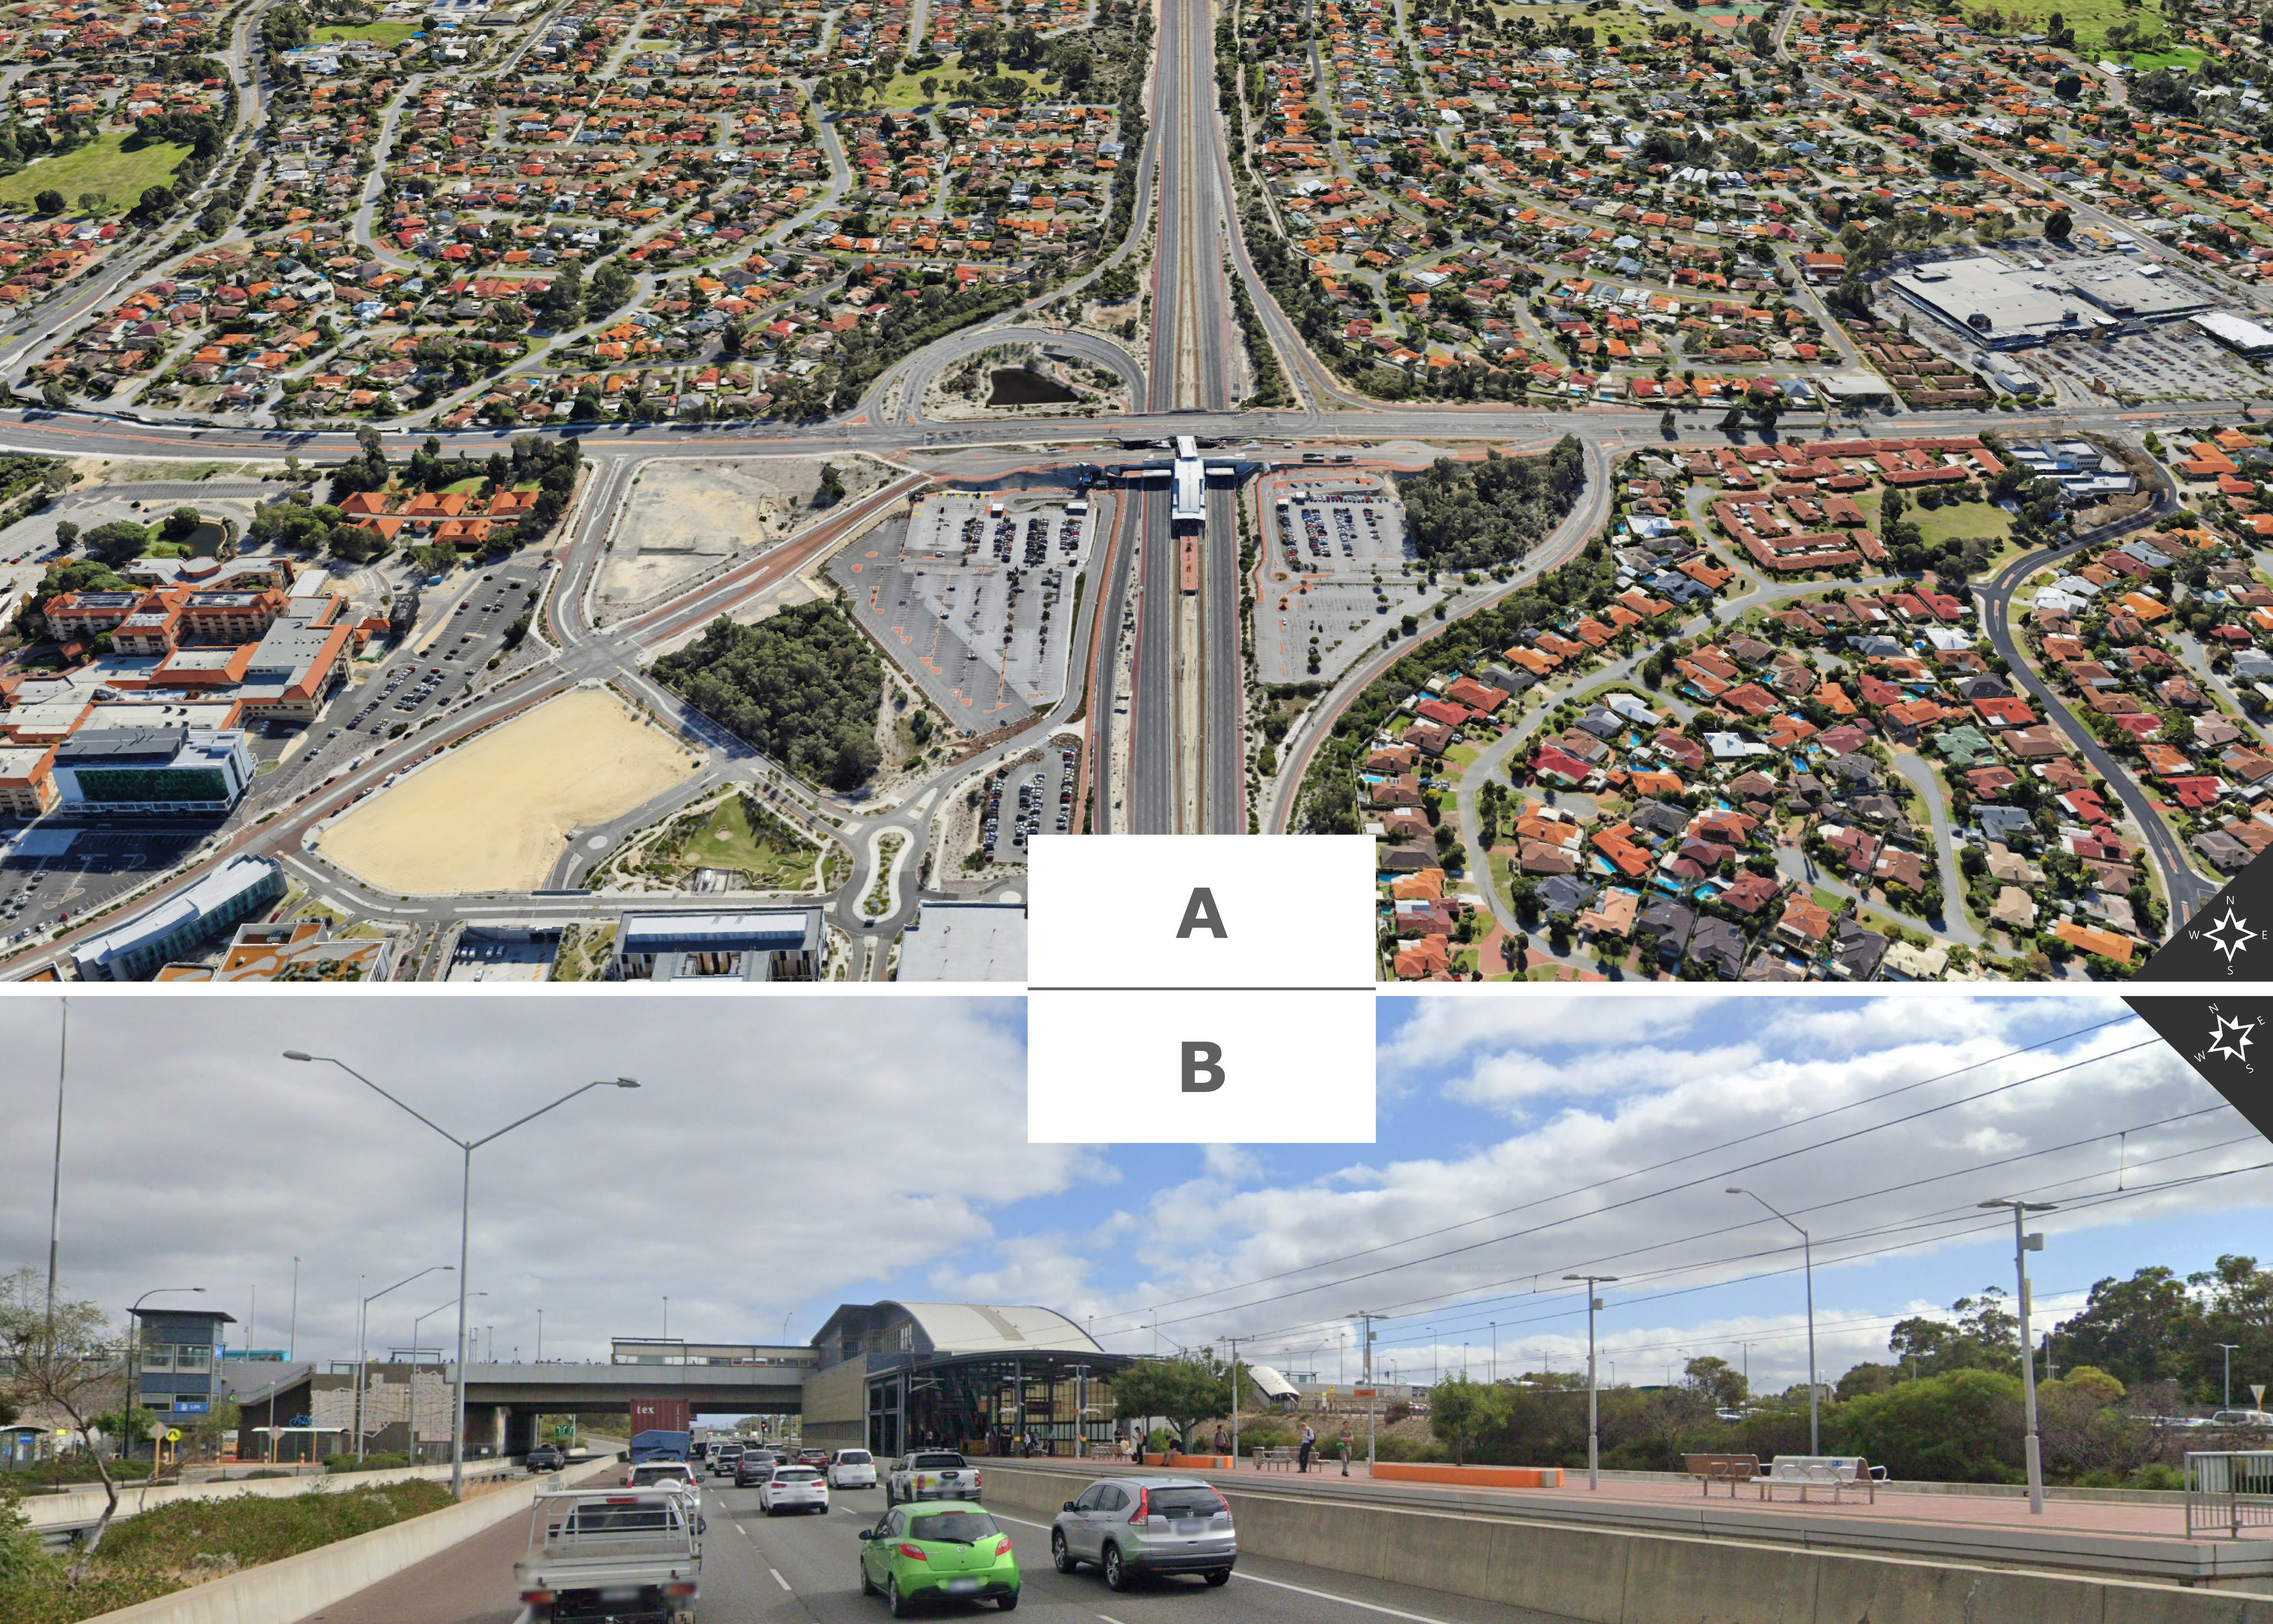
\includegraphics[width=1\columnwidth]{src/Figures/Chap-1/Murdoch.jpg}}
    \vspace{5pt}
    \begin{flushright}\scriptsize{
    Data set (A): Satellite data from \textcolor{blue}{\textcite{google_earth_google_2023}}
    \\
    Data set (B): Images from \Marque{Google Street View} dated November 2023
    }\end{flushright}
\end{figure}

% Adjacent
Consequently, a progressive distinction is made between \acrshort{TOD}\textcolor{blue}{s} that genuinely adhere to the model's principles and those that, due to interpretative or applicative divergences, do not meet the expected criteria. This diversity of approaches has led to the widespread attribution of the \acrshort{TOD} label to a broad range of urban projects that do not necessarily possess all the characteristics of the concept \textcolor{blue}{\autocite[4]{renne_transit-oriented_2013}}\index{Renne, John Luciano|pagebf}\index{Ewing, Reid|pagebf}. Among the reasons for these discrepancies are insufficient pedestrian and cycling amenities, a lack of functional diversity, and excessive automobile parking provision\footnote{~
    Several studies demonstrate that, for a majority of local U.S. authorities, automobile parking remains perceived as a more pertinent mobility and planning solution than densification around transit stations \textcolor{blue}{\autocite[106-107]{cervero_tcrp_2004}}\index{Cervero, Robert|pagebf}\index{Murphy, Steven|pagebf}\index{Ferrell, Christopher|pagebf}\index{Tsai, Yu-Hsin|pagebf}\index{Arrington,~G.~B.|pagebf}\index{Boroski, John|pagebf}\index{Smith-Heimer, Janet|pagebf}\index{Golem, Ron|pagebf}\index{Peninger, Paul|pagebf}\index{Nakajima, Eric|pagebf}\index{Chui, Ener|pagebf}\index{Dunphy, Robert|pagebf}\index{Myers, Mel|pagebf}\index{McKay, Shannon|pagebf}\index{Witenstein, Nicole|pagebf}. Many projects claiming to be \acrshort{TOD}\textcolor{blue}{s} continue to allocate significant space to surface and structured automobile parking, often to maintain existing automobile-centric logics. This persistence of the automobile as the dominant mode results from a lack of framing and reflection on its role in the planning of spaces around stations. Consequently, these \Commas{\textsl{Transit-Oriented Developments} gone wrong} have sometimes allowed the car to remain largely privileged locally \textcolor{blue}{\autocite[39]{bentayou_transit-oriented_2015}}\index{Bentayou, Gilles|pagebf}. Since then, new positions have emerged that place much greater emphasis on the determining role of automobile parking policies in the success of \acrshort{TOD} \textcolor{blue}{\autocite[39]{bentayou_transit-oriented_2015}}\index{Bentayou, Gilles|pagebf}. In particular, by advocating for strengthening regulatory requirements concerning minimum and maximum parking standards, as a reduction in parking ratios for residential projects in \acrshort{TOD}\textcolor{blue}{s} can increase potential density by 20\% to 33\% and reduce parking-related costs by 5\% to 36\%, while promoting affordable prices and improving profitability \textcolor{blue}{\autocite[51-54]{arrington_effects_2008}}\index{Arrington,~G.~B.|pagebf}\index{Cervero, Robert|pagebf}.
}. \textcolor{blue}{\autocites[358]{lund_reasons_2006}[3]{renne_transit-adjacent_2009}}\index{Lund, Hollie~M.|pagebf}\index{Renne, John Luciano|pagebf}. These shortcomings or failures often lead to these projects being more akin to \acrfull{TAD}, i.e., developments that suffer from a lack of connectivity with the public transport network. Furthermore, some projects, designated under the acronym \acrfull{TRD}, exploit proximity to a public transport network for real estate operations without integrating the fundamental principles of \acrshort{TOD} \textcolor{blue}{\autocite[18]{bentayou_transit-oriented_2015}}\index{Bentayou, Gilles|pagebf}. For example, \textcolor{blue}{\textcite[18]{khan_parking_2009}}\index{Khan, Shadhed|pagebf}\index{Bajracharya, Bhishna|pagebf} analyze the Murdoch station, located on the Mandurah line connecting Perth, Australia. The authors identify this site as a typical case of \textsl{Transit-Adjacent Development}, noting that the station's surroundings are largely dominated by highway infrastructure, road interchanges, \acrfull{PnR} facilities, and a sparse suburban fabric. \hyperref[fig-chap1:tad-murdoch]{Figure~\ref{fig-chap1:tad-murdoch}} (page~\pageref{fig-chap1:tad-murdoch}) visually depicts this spatial configuration. These \Commas{\textsl{Transit-Oriented Developments} gone wrong} thus serve as a reminder that proximity to a public transport system and urban density are not sufficient to guarantee the model's success \textcolor{blue}{\autocite[18]{bentayou_transit-oriented_2015}}\index{Bentayou, Gilles|pagebf}.%%Translated%%

% Inspirations
As we have seen, \acrshort{TOD} draws from the struggles and principles of the urban planning movements that preceded it, while readjusting them to meet the challenges of the 21\textsuperscript{st} century. \textcolor{blue}{Peter Calthorpe}, in conceptualizing \acrshort{TOD}, offered urban planning a theoretical framework and a strategic tool with international relevance, whose pertinence is supported by contributions from numerous thinkers in the fields of urbanism and transport \textcolor{blue}{\autocite[111]{almeida_correia_transit-oriented_2020}}\index{Almeida Correia, Gonçalo Homem de|pagebf}\index{Ibraeva, Anna|pagebf}\index{Silva, Cecília|pagebf}\index{Pais Antunes, António|pagebf}. In return, the \acrshort{TOD} model has inspired new approaches in urban development. \textcolor{blue}{Fausto} \textcolor{blue}{\textcite[122]{lo_feudo_scenario_2014}}\index{Lo Feudo, Fausto|pagebf}\index{Menerault, Philippe|pagebf}\index{L'Hostis, Alain|pagebf}\index{Festa, Demetrio Carmine|pagebf} highlights three recent lines of reflection that extend the urban model's legacy by reimagining proximity through a coordinated approach between urbanism and mobility:
\begin{customitemize}
\item The \textsl{compact city}, conceptualized by engineer and researcher \textcolor{blue}{Jean-Louis} \textcolor{blue}{\textcite{maupu_ville_2006}}\index{Maupu, Jean-Louis|pagebf}, is based on a participatory spatial organization integrated into a loop-based framework. This model proposes a balance between urban density and green spaces while promoting a significant modal shift towards public transport networks. The author outlines a vision in which circulations are designed to reduce distances, where density and functional diversity are promoted, and where natural spaces are fully integrated into the urban fabric;
\item The \textsl{pass-through city}, developed by architect and urban planner \textcolor{blue}{David Mangin} and analyzed by \textcolor{blue}{\textcite{masboungi_ville_2008}}\index{Masboungi, Ariella|pagebf}\index{Barbet-Massin, Olivia|pagebf}\index{Mangin, David|pagebf}, places circulation infrastructure at the heart of urban development. These infrastructures are not limited to their utilitarian function but also structure the interaction between neighborhoods through complementarity between spaces of flow and spaces of fixity. The author advocates for a porous and traversable city, facilitating access to daily services through active modes. This model values urban blocks on a human scale and combats barriers to mobility;
\item The \textsl{coherent city}, proposed by \textcolor{blue}{\textcite{korsu_ville_2012}}\index{Korsu, Emre|pagebf}\index{Massot, Marie-Hélène|pagebf}\index{Orfeuil, Jean-Pierre|pagebf}, aims to bring individuals closer to their main activity locations to limit daily travel distances, ideally to less than thirty minutes, with specific application to the Île-de-France region. The authors advocate for a reorganization of urban imbalances, notably by optimizing the distribution of housing and employment;
\item Adding to these three models are the contemporary contributions of \textsl{circular urbanism}, developed by \textcolor{blue}{Sylvain} \textcolor{blue}{\textcite{grisot_manifeste_2020}}\index{Grisot, Sylvain|pagebf}, and the \textsl{15-minute city}, conceptualized by \textcolor{blue}{Carlos} \textcolor{blue}{\textcite{moreno_droit_2020}}\index{Moreno, Carlos|pagebf}. These two urban fabric concepts present theoretical and practical connections with \acrshort{TOD}. The first urban model, that of the \Commas{frugal city} \textcolor{blue}{\autocite[76-80]{chalendar_defi_2021}}\index{Chalendar, Pierre-André de|pagebf}, applies the principles of the circular economy to territorial planning, optimizing resource use and integrating resilient systems into the design and management of urban spaces. The second model focuses on local accessibility, ensuring that essential amenities are accessible within a 15-minute walk or bike ride.
\end{customitemize}%%Translated%%

% 1.1.2. Définition TOD
\needspace{1\baselineskip} % Reserve space
\subsection{The Contours of an Alternative Urban Development Model to the Car-Centric Paradigm
    \label{chap1:tod-presentation-generale-definition}
    }

% Introduction
The strength of rail-oriented urbanism lies in proposing a urban utopia, rethinking planning at the metropolitan or regional scale, at the level of a \Commas{meta-urbanism} \textcolor{blue}{\autocite[346]{lussault_homme_2007}}\index{Lussault, Michel|pagebf}. It is based on multi-scale principles that concretely, albeit not without difficulties, translate into the production of urban projects, leveraging the opportunities offered by connectivity to the transport network \textcolor{blue}{\autocite[58]{lhostis_concevoir_2009}}\index{L'Hostis, Alain|pagebf}\index{Alexandre, Elsa|pagebf}\index{Appert, Manuel|pagebf}\index{Araud-Ruyant, Catherine|pagebf}\index{Basty, Marius|pagebf}\index{Biau, Géraldine|pagebf}\index{Bozzani-Franc, Sandra|pagebf}\index{Boutantin, Gratienne|pagebf}\index{Constantin, Chantal|pagebf}\index{Coralli, Monica|pagebf}\index{Durousset, Marie-Jeanne|pagebf}\index{Fradier, Christophe|pagebf}\index{Gabion, Cyrille|pagebf}\index{Leysens, Thomas|pagebf}\index{Mermoud, Françoise|pagebf}\index{Olny, Xavier|pagebf}\index{Perrin, Emmanuel|pagebf}\index{Robert, Jean|pagebf}\index{Simand, Noémie|pagebf}\index{Stransky, Vaclav|pagebf}\index{Soulas, Claude|pagebf}\index{Verdier, Anne-Marie|pagebf}\index{Vulturescu, Bogdan|pagebf}. The planning concept is ultimately summarized as \Commas{\textsl{a mixed-use community within an average 2,000-foot walking distance of a transit stop and core commercial area. TODs mix residential, retail, office, open space, and public uses in a walkable environment, making it convenient for residents and employees to travel by transit, bicycle, foot, or car.}}\footnote{~
    \Commas{\textsl{Transit-Oriented Development is a mixed-use community within an average 2,000-foot walking distance of a transit stop and core commercial area. TODs mix residential, retail, office, open space, and public uses in a walkable environment, making it convenient for residents and employees to travel by transit, bicycle, foot, or car.}} \textcolor{blue}{\autocite[56]{calthorpe_next_1993}}\index{Calthorpe, Peter|pagebf}.
} \textcolor{blue}{\autocite[56]{calthorpe_next_1993}}\index{Calthorpe, Peter|pagebf}. In other words, the intention behind \acrshort{TOD} is to transform territories into compact, multifunctional spaces oriented towards public transport, with the aim of increasing the use of the public transport network, but also of redeveloping and revitalizing urban areas connected to stations while reducing dependence on individual motorized vehicles and controlling urban sprawl \textcolor{blue}{\autocites[19]{carlton_histories_2007}[7]{tcrp_effects_2008}[112]{almeida_correia_transit-oriented_2020}}\index{Carlton, Ian|pagebf}\index{TCRP@\textsl{TCRP}|pagebf}\index{Almeida Correia, Gonçalo Homem de|pagebf}\index{Ibraeva, Anna|pagebf}\index{Silva, Cecília|pagebf}\index{Pais Antunes, António|pagebf}. According to associated planning strategies, \acrshort{TOD}-type development fulfills a dual purpose. At the local level, it aims to create complete and multifunctional living environments, while at the regional level, the goal is to establish strategic nodes connected to an extensive public transport network. In practice, the urban model mobilizes physical-spatial components to maximize the spatial and socio-economic effects of \acrshort{TOD} \textcolor{blue}{\autocite[39]{conesa_modelisation_2010}}\index{Conesa, Alexis|pagebf}\index{Paris, Didier|pagebf}.%%Translated%%

% 1.1.2.1. 3D
\needspace{1\baselineskip} % Reserve space
\subsubsection*{Evolution of the Principles Guiding the Application of \textsl{Transit-Oriented Development}
    \label{chap1:tod-presentation-generale-definition-principes}
    }

% General Characteristics
To fulfill its ambitions, a \acrshort{TOD}-type project, integrated within a constellation of \acrshort{TOD}\textcolor{blue}{s} \textcolor{blue}{\autocite[42, 56]{calthorpe_next_1993}}\index{Calthorpe, Peter|pagebf}, is defined as an urban planning operation explicitly oriented towards public transport and based on a set of defined characteristics. This type of project generally fits within a perimeter of 600 meters (2,000 feet) around a public transport station, a distance designated as a \Commas{comfortable walking distance} (\Commas{\textsl{a comfortable walking distance}}). However, \textcolor{blue}{Peter} \textcolor{blue}{\textcite[56]{calthorpe_next_1993}}\index{Calthorpe, Peter|pagebf} notes that the size of these neighborhoods should be adjusted on a case-by-case basis, depending on the specificities of each public transport station. The guiding principles of \acrshort{TOD} emphasize urban forms characterized by reinforced density and compactness. These developments promote functional diversity and a mix of uses, structuring the space around stations in a hierarchical organization: a commercial core and offices located closest to the transport infrastructure, followed by public spaces and housing as one moves away from this central hub (see \hyperref[fig-chap1:schema-calthorpe]{Figure~\ref{fig-chap1:schema-calthorpe}}, page~\pageref{fig-chap1:schema-calthorpe}).%%Translated%%

    % Figure TOD schematic
    \begin{carte}[h!]\vspace*{4pt}
        \caption{Original principles of \textsl{Transit-Oriented Development} mapped out.}
        \label{fig-chap1:schema-calthorpe}
        \centerline{\includegraphics[width=1\columnwidth]{src/Figures/Chap-1/EN_Schema_Calthorpe.pdf}}
        \vspace{5pt}
        \begin{flushright}\scriptsize{
        Source: guidelines formulated by \textcolor{blue}{Peter} \textcolor{blue}{\textcite{calthorpe_next_1993}}\index{Calthorpe, Peter|pagebf}
        \\
        Graphic adaptation: \textcolor{blue}{Dylan Moinse (2021)}
        }\end{flushright}
    \end{carte}

    % Secondary Area
In the immediate periphery, the author introduces a \Commas{Secondary Area}, intended for low-density uses such as residential subdivisions, schools, activities with a large spatial footprint, and large parks (see \hyperref[fig-chap1:schema-calthorpe]{Figure~\ref{fig-chap1:schema-calthorpe}}, page~\pageref{fig-chap1:schema-calthorpe}). These \Commas{secondary areas} enhance the viability and attractiveness of the \acrshort{TOD} by integrating complementary functions \textcolor{blue}{\autocite[42, 60, 87]{calthorpe_next_1993}}\index{Calthorpe, Peter|pagebf}. Within these projects, the development aims to encourage the use of public transportation and non-motorized travel modes through thoughtful infrastructure integration and urban design that promotes these behaviors.%%Translated%%

    % Original principles
To explain the foundations of \acrshort{TOD}, \textcolor{blue}{Peter} \textcolor{blue}{\textcite[43]{calthorpe_next_1993}}\index{Calthorpe, Peter|pagebf} summarizes this approach into seven original principles: (i) organize regional growth in a compact manner favorable to the public transport system; (ii) locate commercial, residential, recreational, and administrative activities within walking distance of transit stations; (iii) design pedestrian-friendly street networks that directly connect local destinations; (iv) offer a variety of housing types, densities, and costs; (v) preserve open and natural spaces; (vi) orient neighborhoods and buildings around public spaces; and (vii) encourage densification and revitalization of neighborhoods along existing transport corridors.%%Translated%%

    % TOD typology
These principles apply differently depending on whether it is an \Commas{Urban \acrshort{TOD}} or a \textsl{Neighborhood \acrshort{TOD}}, as shown in \hyperref[fig-chap1:schema-calthorpe]{Figure~\ref{fig-chap1:schema-calthorpe}} (page~\pageref{fig-chap1:schema-calthorpe}). The first type of transit-oriented neighborhood is served by a structuring transport system such as a heavy or light rail network or \acrfull{BRT}. This strategic \Commas{urban} space must accommodate significant flows by concentrating jobs and intensifying land use through high or medium density and functional diversity, dominated by offices and businesses that generate traffic \textcolor{blue}{\autocite[57]{calthorpe_next_1993}}\index{Calthorpe, Peter|pagebf}. The second type is associated with local bus service that allows connection to the structuring network in less than ten minutes or within five kilometers, thanks to high service frequency. This strategic \Commas{residential} space can develop in the form of corridors with medium housing density and some functional diversity \textcolor{blue}{\autocite[57]{calthorpe_next_1993}}\index{Calthorpe, Peter|pagebf}. \textcolor{blue}{Peter} \textcolor{blue}{\textcite[50, 61]{calthorpe_next_1993}}\index{Calthorpe, Peter|pagebf} also identifies three main types of \acrshort{TOD} fabrication based on their location: \Commas{redevelopable sites}, existing urban areas suitable for revitalization; \Commas{infill sites} corresponding to open spaces or vacant lots integrated into the existing urban fabric; and \Commas{New Growth Areas}, located in the urban periphery, which are the easiest to develop but contribute to increased urban sprawl.%%Translated%%

    % 3D list
Based on these principles, numerous academic works have sought to conceptualize and enrich the \acrshort{TOD}, notably by introducing analytical frameworks aimed at deepening its theoretical foundations. Although there is no universal consensus around a single definition of \acrshort{TOD}, the notion of the \Commas{3Ds}, introduced by \textcolor{blue}{\textcite[216]{cervero_travel_1997}}\index{Cervero, Robert|pagebf}\index{Kockelman, Kara|pagebf}, constitutes a frequently used basis in the literature:
    \begin{customitemize}
\item \textsl{Density}. This first dimension corresponds to the variable of interest per unit area, whether it be inhabitants, households, dwellings, or jobs. It reflects the concentration of people and activities, a \Commas{well-designed, well-managed density} (\textcolor{blue}{\textcite{cervero_panorama_2012}}\index{Cervero, Robert|pagebf}, cited by \textcolor{blue}{\textcite[127]{lo_feudo_scenario_2014}}\index{Lo Feudo, Fausto|pagebf}\index{Menerault, Philippe|pagebf}\index{L'Hostis, Alain|pagebf}\index{Festa, Demetrio Carmine|pagebf});
\item \textsl{Functional Diversity}. This second dimension evaluates the degree of land use mix;
\item \textsl{Design}. This third dimension encompasses street characteristics, the organization of circulation and parking spaces, urban forms, and urban quality.
    \end{customitemize}%%Translated%%

    % 3Ds description
These three dimensions are interdependent and act synergistically to support dense and multifunctional urban development, where pedestrian mobility is prioritized and travel is reduced in terms of quantity and average distance due to the proximity of urban activities to residential areas. The \gls{design}, which seems to have the most significant effects on public transport use \textcolor{blue}{\autocite[107]{ewing_travel_2001}}\index{Ewing, Reid|pagebf}\index{Cervero, Robert|pagebf}, improves the connectivity of various urban functions. Ultimately, the \Commas{3Ds} support the integrated vision of dense and multifunctional urban development that provides an accessible and high-quality system \textcolor{blue}{\autocites[216]{cervero_travel_1997}[107]{ewing_travel_2001}}\index{Cervero, Robert|pagebf}\index{Kockelman, Kara|pagebf}\index{Ewing, Reid|pagebf}\index{Cervero, Robert|pagebf}.%%Translated%%

    % 6D/7D
Beyond the triad usually integrated into the urban model, other parameters gradually enrich the analytical frameworks related to \acrshort{TOD}. To mention only the most recognized and widespread dimensions in the analytical grids adopted for \acrshort{TOD}, three new aspects emerged progressively between 2001 and 2010 \textcolor{blue}{\autocite[267]{ewing_travel_2010}}\index{Ewing, Reid|pagebf}\index{Cervero, Robert|pagebf}: \textsl{Destination accessibility}, which evaluates the ease of access to various urban amenities such as workplaces, services, shops, or public facilities; \textsl{Distance to transit}, which measures the ease of spatial connection to the public transport network; and \textsl{Demand management}, although often marginalized in studies \textcolor{blue}{\autocite[267]{ewing_travel_2010}}\index{Ewing, Reid|pagebf}\index{Cervero, Robert|pagebf}, which covers all public policies and initiatives aimed at reducing the actual use of private cars, particularly regarding the availability of car parking spaces. These three determinants of public transport demand thus expand the analytical framework to the \Commas{5Ds}, or even the \Commas{6Ds} \textcolor{blue}{\autocite[4-6]{thomas_transit-oriented_2020}}\index{Thomas, Ren|pagebf}\index{Bertolini, Luca|pagebf}. It should be noted that many other parameters have been explored in various scientific productions, such as the socio-demographic characteristics of the population or users (\textsl{Demographics}) \textcolor{blue}{\autocite[75]{ewing_trip_2017}}\index{Ewing, Reid|pagebf}\index{Tian, Guang|pagebf}\index{Lyons, Torrey|pagebf}\index{Terzano, Kathryn|pagebf} or the attractiveness of the public transport network expressed in terms of efficiency and comfort (\textsl{Desirability of transit}) \textcolor{blue}{\autocite[8]{mangu_evaluation_2025}}\index{Mangu, Sriram|pagebf}\index{Kadali,~B. Raghuram|pagebf}\index{Subbarao, Saladi~S.~V.|pagebf}\index{Lin, Jen-Jia|pagebf}.%%Translated%%

    % Interweaving of supply- and demand-oriented strategies
Thus, the founding principles of \acrshort{TOD} can be summarized around a multiscale action on territorial configurations and, more specifically, on the urban environment. This is reflected in the coexistence of two complementary approaches that maximize its effectiveness. The first strategy is supply-oriented, known as \acrfull{TSM}, and the second is demand-oriented, known as \acrfull{TDM} \textcolor{blue}{\autocite[67]{cervero_transit_1998}}\index{Cervero, Robert|pagebf}.

    % Transportation Systems Management
The \acrshort{TSM} strategy aims to reorganize the mobility system at a lower cost by optimizing existing infrastructure and services. This eco-mobility approach can rely on direct interventions in the urban environment, such as those described by the \Commas{3Ds}. These interventions not only intensify the use of public transport but also generate better-distributed bidirectional flows over time \textcolor{blue}{\autocite[4]{grigolon_transit-oriented_2016}}\index{Grigolon, Anna Beatriz|pagebf}\index{Koeva, Mila|pagebf}\index{Madureira, Ana Mafalda|pagebf}\index{Singh, Yamini~J.|pagebf}. Furthermore, the use of \acrfull{ICT} is part of this strategy, facilitating coordinated and real-time management of mobility flows at a reduced cost. Among the technologies employed are traffic optimization, real-time data provision and management, and vehicle geolocation \textcolor{blue}{\autocite[96]{cervero_transit_1998}}\index{Cervero, Robert|pagebf}.%%Translated%%

    % Transportation Demand Management
The \acrshort{TDM} strategy, on the other hand, relies more on measures aimed at reducing car use and ownership and encouraging a modal shift towards alternative mobility systems. These measures include coercive devices such as traffic and parking moderation, urban congestion taxation, or the introduction of environmental standards, such as those related to fuel consumption. An emblematic example of this demand-oriented strategy is the Dutch concept of \textsl{woonerven}\footnote{~
    The \textsl{woonerf} concept, literally \Commas{residential courtyard}, refers to a shared space that prioritizes pedestrians, cyclists, and neighborhood life. Traffic calming is ensured by physical obstacles such as vegetation or urban furniture, and by a shared roadway that blurs the boundaries between different types of users, promoting driver vigilance \textcolor{blue}{\autocite[3]{collarte_woonerf_2012}}\index{Collarte, Natalia|pagebf}.
}. However, this approach is not limited to restrictive measures. By seeking to influence mobility behaviors, incentive actions such as implementing staggered working hours or financial aid encouraging the use of alternative modes contribute to this logic \textcolor{blue}{\autocite[97]{cervero_transit_1998}}\index{Cervero, Robert|pagebf}.%%Translated%%

% 1.1.2.2. Expected Effects
\needspace{1\baselineskip} % Reserve space
\subsubsection*{Expected Benefits of \textsl{Transit-Oriented Development}
    \label{chap1:tod-presentation-generale-definition-effets-attendus}
    }

% Objectives
The \acrshort{TOD} now serves as both a project territory and an urban action tool for many local authorities \textcolor{blue}{\autocite[23]{bentayou_transit-oriented_2015}}\index{Bentayou, Gilles|pagebf}. This development model engages institutions and organizations, ranging from economic development actors, social economy, public health, to the educational sector, who embrace the concept and actively participate in producing practical guides or various feedback\footnote{~
    A survey conducted by the U.S. transportation company \textcolor{blue}{\textcite[9]{hntb_america_2016}}, involving 1,000 participants, examined the expected benefits of implementing a \acrshort{TOD} project. It highlighted a reduction in car dependency (57\%), a return to proximity (46\%), a decrease in carbon footprint (44\%), improved access to services (43\%) and jobs (37\%), economic revitalization (43\%), better connectivity between territories (42\%), and urban area regeneration (30\%).
}. The expected effects of \acrshort{TOD}, as defined by its main promoter, the \textcolor{blue}{Center for Transit-Oriented Development}\index{Center for Transit-Oriented Development@\textsl{Center for Transit-Oriented Development}|pagebf} \textcolor{blue}{\autocites[35-39]{ohland_communicating_2006}[11-21]{noland_measuring_2014}}\index{Ohland, Gloria|pagebf}\index{Gorewitz, Cali|pagebf}\index{Noland, Robert~B.|pagebf}\index{Ozbay, Kaan|pagebf}\index{DiPetrillo, Stephanie|pagebf}\index{Iyer, Shri|pagebf}, can be described as follows \textcolor{blue}{\autocites[11]{bentayou_transit-oriented_2015}[114-122]{ibraeva_transit-oriented_2020}[5-11]{ali_dynamics_2021}[6-11]{wan_equity_2023}}\index{Bentayou, Gilles|pagebf}\index{Ibraeva, Anna|pagebf}\index{Almeida Correia, Gonçalo Homem de|pagebf}\index{Silva, Cecília|pagebf}\index{Antunes, António Pais|pagebf}\index{Ali, Liaqat|pagebf}\index{Nawaz, Ahsan|pagebf}\index{Iqbal, Shahid|pagebf}\index{Aamir Basheer, Muhammad|pagebf}\index{Haameed, Javaria|pagebf}\index{Albasher, Gadah|pagebf}\index{Shah, Syyed Adnan Raheel|pagebf}\index{Bai, Yong|pagebf}:
    \begin{customitemize}
\item \textsl{Modal shift from individual car use}. Reduce car usage to increase public transport ridership, contributing to a reduction in negative externalities associated with motorized traffic;
\item \textsl{Preservation of the environment and natural resources}. Reduce \acrfull{GHG} emissions and various forms of pollution generated by cars, while limiting excessive soil sealing due to uncontrolled urban sprawl. Improve public health quality, both physical and mental;
\item \textsl{Improvement of urban living conditions}. Develop neighborhoods that promote an active and healthy lifestyle, enhancing dynamic and lively territories and reducing urban congestion and road accidents. Foster the emergence of vibrant and attractive communities;
\item \textsl{Reduction of socio-spatial segregation}. Encourage the development of decentralized urban hubs, reducing dependence on metropolitan centers and long commutes. Strengthen the appropriation of territories that build identities;
\item \textsl{Promotion of social equity}. Enhance access to employment and opportunities for low-income populations;
\item \textsl{Better management of economic and budgetary costs}. Reduce collective costs passed on to society and the share of household income spent on mobility expenses. Increase revenue generated from public transport operations and real estate promotion.
    \end{customitemize}%%Translated%%

% Modal Shift from Car Use
\textsl{Modal shift from individual car use}. In terms of mobility behavior changes, most literature dedicated to \acrshort{TOD} suggests that individuals living and, or working in \acrshort{TOD} neighborhoods use cars less compared to the rest of the population. They rely more on public transportation and active modes: studies show that between 25\% and 50\% of residents in developed station neighborhoods regularly use public transportation \textcolor{blue}{\autocites[61]{lund_travel_2004}[40]{evans_transit-oriented_2007}[5, 15]{cervero_vehicle_2008}[62]{kamruzzaman_advance_2014}[152]{kamruzzaman_patterns_2014}}\index{Lund, Hollie~M.|pagebf}\index{Cervero, Robert|pagebf}\index{Wilson, Richard~W.|pagebf}\index{Evans, James|pagebf}\index{Pratt, Richard|pagebf}\index{Stryker, Andrew|pagebf}\index{Kuzmyak,~J.|pagebf}\index{Cervero, Robert|pagebf}\index{Arrington,~G.~B.|pagebf}\index{Kamruzzaman, Md.|pagebf}\index{Baker, Douglas|pagebf}\index{Washington, Simon|pagebf}\index{Turrell, Gavin|pagebf}\index{Wood, Lisa|pagebf}\index{Hine, Julian|pagebf}\index{Currie, Graham|pagebf}\index{Giles-Corti, Billie|pagebf}. This figure is generally three to four times higher than the average observed in the rest of the metropolitan area, with a similar trend noted for walking and cycling. Consequently, we observe a halving of car trips in U.S. \acrshort{TOD} neighborhoods \textcolor{blue}{\autocite[14]{cervero_vehicle_2008}}\index{Cervero, Robert|pagebf}\index{Arrington,~G.~B.|pagebf}. However, about 40\% of this effect can be attributed to self-selection bias, where individuals moving near public transport networks are already predisposed to use them \textcolor{blue}{\autocites[2082]{cervero_transit-oriented_2007}[50]{laham_nonwork_2017}}\index{Cervero, Robert|pagebf}\index{Laham, Maria Luz|pagebf}\index{Noland, Robert~B.|pagebf}. Another notable effect is the reduction in car ownership rates. Populations in \acrshort{TOD} neighborhoods have an almost two times smaller car fleet compared to areas not oriented towards public transport \textcolor{blue}{\autocite[50]{arrington_effects_2008}}\index{Arrington,~G.~B.|pagebf}\index{Cervero, Robert|pagebf}, although these proportions vary depending on the specific characteristics of each studied territory \textcolor{blue}{\autocite[79]{lund_travel_2004}}\index{Lund, Hollie~M.|pagebf}\index{Cervero, Robert|pagebf}\index{Wilson, Richard~W.|pagebf}.%%Translated%%

% Environmental Preservation
\textsl{Preservation of the environment and natural resources}. The scientific literature on the effects of \acrshort{TOD} in reducing pollution and controlling suburban sprawl remains limited \textcolor{blue}{\autocite[11]{ashik_investigating_2022}}\index{Ashik,~F.~R.|pagebf}\index{Rahman,~M.~H.|pagebf}\index{Kamruzzaman, Md.|pagebf}. However, several studies provide compelling evidence. It has been demonstrated that metropolitan areas adopting \acrshort{TOD} policies tend to improve air quality, primarily due to the reduction in total distance traveled by car \textcolor{blue}{\autocite[20]{gu_transit-oriented_2019}}\index{Gu, Peiqin|pagebf}\index{He, Dongxu|pagebf}\index{Chen, Yulin|pagebf}\index{Zegras, Pericles~C.|pagebf}\index{Jiang, Yang|pagebf}. These results highlight the strong performance of these policies in terms of sustainability \textcolor{blue}{\autocite[109]{choi_influence_2018}}\index{Choi, Kwangyul|pagebf}. In Los Angeles, the opening of a new light rail line led to a 27\% reduction in daily \acrshort{GHG} emissions related to the mobility of households residing less than 800 meters from the stops \textcolor{blue}{\autocite[13]{boarnet_can_2017}}\index{Boarnet, Marlon~G.|pagebf}\index{Wang, Xize|pagebf}\index{Houston, Douglas|pagebf}. Another study in the same region reports a 30\% to 36\% decrease in emissions of suspended and fine particles, as well as other respiratory irritants in \acrshort{TOD} areas, compared to low-density areas. These results are mainly explained by better accessibility to public transport infrastructure, leading to reduced energy consumption and shorter travel distances \textcolor{blue}{\autocite[25]{nahlik_transit-oriented_2014}}\index{Nahlik, Matthew~J.|pagebf}\index{Chester, Mikhail~V.|pagebf}. In Charlotte, a model implemented by \textcolor{blue}{\textcite[4]{hosseini_understanding_2024}}\index{Hosseini, Sanaz Sadat|pagebf}\index{Ardabili, Babak Rahimi|pagebf}\index{Azarbayjani, Mona|pagebf}\index{Pulugurtha, Srinivas|pagebf}\index{Pulugurtha, Hamed|pagebf} highlights an 8\% to 21\% reduction in daily emissions during peak hours in the scenario where bus ridership is doubled, a proportion that can rise to 37\% in the most favorable \acrshort{TOD} scenario. Furthermore, \textcolor{blue}{\textcite[120]{kamruzzaman_investigating_2018}}\index{Kamruzzaman, Md.|pagebf}\index{Deilami, Kaveh|pagebf}\index{Yigitcanlar, Tan|pagebf} show that \acrshort{TOD} policies have helped limit uncontrolled urban sprawl in Brisbane. However, these areas exhibit the most intense urban heat island effects in the metropolis, due to an imbalance in the distribution of green and natural spaces.%%Translated%%

% Quality of Life Improvement
\textsl{Improvement of urban living conditions, in terms of public health and well-being}. By promoting better air quality and encouraging physical activity, it plays a crucial role in fostering healthier lifestyles. Indeed, the use of public transportation is associated with lower levels of sedentary behavior, especially when urban forms encourage active modes \textcolor{blue}{\autocites[58]{knell_transit_2017}[22]{frank_quantifying_2022}}\index{Knell, Gregory|pagebf}\index{Durand, Casey~P.|pagebf}\index{Shuval, Kerem|pagebf}\index{Kohl, Harold~W.|pagebf}\index{Salvo, Deborah|pagebf}\index{Sener, Ipek|pagebf}\index{Gabriel, Kelley Pettee|pagebf}\index{Frank, Lawrence~D.|pagebf}\index{Fow, Eric~H.|pagebf}\index{Ulmer, Jared~M.|pagebf}\index{Chapman, James~E.|pagebf}\index{Braun, Lindsay~M.|pagebf}. By improving the quality of the urban environment, residents of \acrshort{TOD} neighborhoods are less exposed to pollution and are more active \textcolor{blue}{\autocites[12-13]{belzer_transit-oriented_2002}[215]{cervero_green_2011}[271]{guerra_cost_2011}}\index{Belzer, Dena|pagebf}\index{Autler, Gerald|pagebf}\index{Cervero, Robert|pagebf}\index{Sullivan, Cathleen|pagebf}\index{Guerra, Erick|pagebf}. Furthermore, these urban projects contribute to the redevelopment of public spaces and the regeneration of territories, enhancing urban quality and strengthening their residential, tourist, and economic attractiveness \textcolor{blue}{\autocites[9]{ratner_reshaping_2010}[109-112]{ferbrache_city_2017}}\index{Ratner, Keith~A.|pagebf}\index{Goetz, Andrew~R.|pagebf}\index{Ferbrache, Fiona|pagebf}\index{Knowles, Richard~D.|pagebf}. An emblematic example is the \Commas{Grenoble effect}, considered a model of urban revitalization. Since 1987, Grenoble has reintroduced a tramway system coupled with an ambitious urban project connecting the station to the new campus. This project has served as a reference for many cities in France and around the world \textcolor{blue}{\autocites[7]{boquet_renaissance_2017}[37]{hass-klau_economic_2004}}\index{Boquet, Yves|pagebf}\index{Hass-Klau, Carmen|pagebf}\index{Crampton,~G.|pagebf}\index{Benjari, Rabia|pagebf}. \acrshort{TOD} also strengthens the sense of community \textcolor{blue}{\autocite[231-248]{dittmar_new_2003}}\index{Dittmar, Hank|pagebf}\index{Ohland, Gloria|pagebf} and the mobility and residential satisfaction of residents \textcolor{blue}{\autocite[86]{curtis_transit_2009}}\index{Curtis, Carey|pagebf}\index{Renne, John Luciano|pagebf}\index{Bertolini, Luca|pagebf}. Although public transportation is often perceived as less pleasant than driving or active modes, \acrshort{TOD} has the capacity to reverse this sensory and cognitive appreciation by improving user comfort and experience \textcolor{blue}{\autocites[258-259]{olsson_happiness_2013}[287-288][79]{wu_does_2014}{majumdar_identification_2021}}\index{Olsson, Lars~E.|pagebf}\index{Gärling, Tommy|pagebf}\index{Ettema, Dick|pagebf}\index{Friman, Margareta|pagebf}\index{Fuji, Satoshi|pagebf}\index{Majumdar, Bandhan Bandhu|pagebf}\index{Jayakumar, Malavika|pagebf}\index{Sahu, Prasanta~K.|pagebf}\index{Potoglou, Dimitris|pagebf}\index{Wu, Wenjie|pagebf}.%%Translated%%

% Reduction of socio-spatial segregation
\textsl{Reduction of socio-spatial segregation and promotion of social equity}. The \acrshort{TOD} is part of an urban regeneration dynamic, enhancing the residential and economic attractiveness of certain neighborhoods. In particular, former deindustrialized areas benefit from this opportunity to be revitalized. Notable examples include the London Docklands and Salford Quays in England, as well as Baltimore in the United States \textcolor{blue}{\autocites[42, 46, 68]{knowles_investigation_2014}[6]{knowles_evaluation_2016}}\index{Knowles, Richard~D.|pagebf}\index{Ferbrache, Fiona|pagebf}. Through its polycentric approach, \acrshort{TOD} supports not only the local economy but also regional competitiveness by optimizing land use \textcolor{blue}{\autocite[40]{litman_evaluating_2011}}\index{Litman, Todd|pagebf}. However, this dynamic has ambivalent effects. One of the major risks is gentrification, which results from the appreciation of property values in station neighborhoods and leads to rising housing costs\footnote{~
    This phenomenon, increasingly documented in the literature, has sparked numerous debates over the past decade \textcolor{blue}{\autocite[738]{padeiro_transit-oriented_2019}}\index{Padeiro, Miguel|pagebf}\index{Louro, Ana|pagebf}\index{Costa, Nuno Marques de|pagebf}. Sometimes clearly characterized in relation to rising land prices \textcolor{blue}{\autocite[14-15]{wu_impacts_2020}}\index{Wu, Wenjie|pagebf}\index{Zheng, Siqi|pagebf}\index{Wang, Bing|pagebf}\index{Du, Minzhe|pagebf}, sometimes absent—generally when \acrshort{TOD} is combined with an affordable housing policy \textcolor{blue}{\autocite[16]{dawkins_transit-induced_2016}}\index{Dawkins, Casey|pagebf}\index{Moeckel, Rolf|pagebf}. Defining its extent or generalizing its effects remains challenging, as evidenced by numerous recent studies on this subject \textcolor{blue}{\autocites{cook_light_2019}{padeiro_transit-oriented_2019}{ewing_is_2022}{wan_equity_2023}}\index{Cook, Justin|pagebf}\index{Padeiro, Miguel|pagebf}\index{Louro, Ana|pagebf}\index{Costa, Nuno Marques de|pagebf}\index{Wan, Tianyue|pagebf}\index{Lu, Wei|pagebf}\index{Sun, Peijin|pagebf}\index{Ewing, Reid|pagebf}\index{Sabouri, Sadegh|pagebf}\index{Kaniewsk, Justyna|pagebf}\index{Ameli, Hassan|pagebf}\index{Yang, Wookjae|pagebf}\index{Kiani, Fatemeh|pagebf}\index{Kim, Junsik|pagebf}\index{Chibamba, Douty|pagebf}.
}. According to \textcolor{blue}{Gilles} \textcolor{blue}{\textcite[32]{bentayou_transit-oriented_2015}}\index{Bentayou, Gilles|pagebf}, it would be incorrect to reduce the social consequences of \acrshort{TOD} to gentrification alone, as the urban model is inherently designed to create or restore value to areas located near transport hubs. If local authorities act proactively, they can counter these adverse effects by implementing policies that promote the development of affordable housing and control capital gains through land price and rent regulation \textcolor{blue}{\autocites[17]{litman_evaluating_2011}[32]{bentayou_transit-oriented_2015}{yu_valueadded_2018}[463]{harrison_corridors_2019}{ewing_is_2022}}\index{Bentayou, Gilles|pagebf}\index{Litman, Todd|pagebf}\index{Yu, Haitao|pagebf}\index{Pang, Hao|pagebf}\index{Zhang, Ming|pagebf}\index{Ewing, Reid|pagebf}\index{Sabouri, Sadegh|pagebf}\index{Kaniewsk, Justyna|pagebf}\index{Ameli, Hassan|pagebf}\index{Yang, Wookjae|pagebf}\index{Kiani, Fatemeh|pagebf}\index{Kim, Junsik|pagebf}\index{Chibamba, Douty|pagebf}\index{Harrison, Philip|pagebf}\index{Rubin, Margot|pagebf}\index{Appelbaum, Alexandra|pagebf}\index{Dittgen, Romain|pagebf}.%%Translated%%

% Better management of economic costs
\textsl{Economic advantages and cost control}. From a societal perspective, \acrshort{TOD} represents an opportunity to reduce collective costs. The decrease in road accidents, lower exposure to pollution, and the reduction of urban network sprawl all contribute to easing public expenses \textcolor{blue}{\autocite[17]{litman_evaluating_2011}}\index{Litman, Todd|pagebf}. At the local level, and more specifically in station neighborhoods, economic revitalization is often observed. These strategic locations stimulate both public and private investments, while encouraging the reorganization of economic centralities \textcolor{blue}{\autocites[89]{knowles_investigation_2014}[6]{knowles_evaluation_2016}}\index{Knowles, Richard~D.|pagebf}\index{Ferbrache, Fiona|pagebf}. Along public transport lines, studies have shown a significant increase in new businesses near stations, with growth rates doubled compared to non-accessible areas. On the other hand, industrial activities tend to decrease in these same spaces \textcolor{blue}{\autocites{duncan_impact_2011}{credit_transit-oriented_2018}}\index{Duncan, Michael|pagebf}\index{Credit, Kevin|pagebf}. At the household level, a notable effect of \acrshort{TOD} is the reduction of mobility expenses. The share of income spent on transportation can decrease from 25\% to only 9\%, as observed in the United States \textcolor{blue}{\autocites[25]{beauvais_amenagements_2017}[25]{nahlik_transit-oriented_2014}[38]{ohland_communicating_2006}}\index{Beauvais, Jean-Marie|pagebf}\index{Nahlik, Matthew~J.|pagebf}\index{Chester, Mikhail~V.|pagebf}\index{Ohland, Gloria|pagebf}\index{Gorewitz, Cali|pagebf}.%%Translated%%

% Transition
As we have seen, \acrshort{TOD} always refers to the idea of densification and diversification of urban functions around public transport hubs, with the aim of generating societal benefits. However, depending on the institutions that promote it or seek to implement it, \acrshort{TOD} can serve a variety of objectives: concerns related to public health, improvement of urban spaces, combating urban congestion, supporting the local economy, or providing affordable housing. This diversity of goals or expected benefits from \acrshort{TOD} projects \textcolor{blue}{s} largely explains the success and spread of this development model \textcolor{blue}{\autocite[14]{bentayou_transit-oriented_2015}}\index{Bentayou, Gilles|pagebf}. Highly internationalized, this model has been adapted to the specificities of the geographical, political, and technical contexts in which it has been implemented \textcolor{blue}{\autocites[1202]{thomas_is_2018}[181]{veloso_e_zarate_quartiers_2024}}\index{Thomas, Ren|pagebf}\index{Pojani, Dorina|pagebf}\index{Lenferink, Sander|pagebf}\index{Bertolini, Luca|pagebf}\index{Stead, Dominic|pagebf}\index{Krabben, Erwin van der|pagebf}\index{Veloso e Zarate, Halina|pagebf}\index{Triggianese, Manuela|pagebf}\index{Baron, Nacima|pagebf}\index{Le Bot, Nils|pagebf}\index{Detavernier, Pauline|pagebf}. And this is certainly the strength of \acrshort{TOD}, which can be interpreted and reinterpreted depending on the context. As \textcolor{blue}{Mounya} \textcolor{blue}{\textcite[52]{el_hadeuf_ville_2017}}\index{El Hadeuf, Mounya|pagebf}\index{Laterrasse, Jean|pagebf} explains, the absence of a predefined recipe fixed in stereotypes of standardized \acrshort{TOD} neighborhoods helps avoid \Commas{\textsl{complacency in the search for new urban compositions}}.%%Translated%%

% 1.1.3.
\needspace{1\baselineskip} % Reserve space
\subsection{Applications and adaptations of \textsl{Transit-Oriented Development}
    \label{chap1:tod-presentation-generale-declinaisons}
    }

    % Introduction
The significant increase in the number of scientific contributions on \acrshort{TOD} over the past decade reflects the renewed relevance of this action-research topic \textcolor{blue}{\autocite[2545]{jain_systematic_2020}}\index{Jain, Deepshikha|pagebf}\index{Singh, Ekta|pagebf}\index{Ashtt, Rashmi|pagebf}. Since the beginning of the 21\textsuperscript{st} century, there has been a global resurgence of interest in \acrshort{TOD}, driven by the diversification of transport modes, which challenges the traditional dichotomy between public and private transport \textcolor{blue}{\autocite[3]{knowles_transit_2019}}\index{Knowles, Richard~D.|pagebf}\index{Ferbrache, Fiona|pagebf}. This ever-evolving urban model is seen as a potential lever to promote \Commas{smart urban growth} and foster urban regeneration dynamics, both in developed countries and emerging economies \textcolor{blue}{\autocite[2191]{goetz_suburban_2013}}\index{Goetz, Andrew~R.|pagebf}. Due to the many variations of \acrshort{TOD} in diverse contexts, this planning concept offers an opportunity for reflection on cross-cutting themes such as territorial attractiveness and valorization \textcolor{blue}{\autocite[34]{stransky_periurbain_2019}}\index{Stransky, Vaclav|pagebf}. This multiplicity of applications, reflecting the adaptability of \acrshort{TOD}, enriches both the scientific and technical literature and the operational projects that advocate for it around the world, even if these projects are often referred to by other terms, such as in France. Given the large number of state-of-the-art reviews and literature surveys that have already compared international approaches, this thesis does not aim to provide an exhaustive description of them. Rather, it seeks to highlight the conceptual and practical adaptability of \acrshort{TOD}, through the analysis of its fundamental principles and its multiple forms of application, with the goal of clarifying the strategic role that bicycles and their variants can play.%%Translated%%

% 1.1.3.1. Planning tools
\needspace{1\baselineskip} % Reserve space
\subsubsection*{French Contractualization of \textsl{Transit-Oriented Development} Projects
    \label{chap1:tod-presentation-generale-definition-instruments}
    }

    % Introduction
Due to its encompassing nature, involving various sectors and spatial scales, \acrshort{TOD} engages a multitude of actors. Among them are supranational, national, or regional entities responsible for legislation and funding; local authorities in charge of land use planning and regulations; mobility agencies responsible for planning and operating transport systems; as well as landlords and real estate developers, who ensure the production of housing \textcolor{blue}{\autocite[8]{mathur_promoting_2020}}\index{Mathur, Shishir|pagebf}\index{Gatdula, Aaron|pagebf}. It is within this context that \textcolor{blue}{\textcite[152]{thomas_defining_2017}}\index{Thomas, Ren|pagebf}\index{Bertolini, Luca|pagebf} published a meta-analysis on the applicability of the planning concept, listing the key success factors of \acrshort{TOD}: political stability as well as the existence of a regional intersectoral dialogue space and an interdisciplinary network of regional stakeholders. However, persistent gaps common to many countries hinder the operationalization of this urban model. These include a lack of cooperation and integration between stakeholders, an absence of institutionalization of this coordination, and governance lacking continuity \textcolor{blue}{\autocite[124]{ibraeva_transit-oriented_2020}}\index{Ibraeva, Anna|pagebf}\index{Almeida Correia, Gonçalo Homem de|pagebf}\index{Silva, Cecília|pagebf}\index{Antunes, António Pais|pagebf}. In response to the sectoral and geographical fragmentation of competencies, various strategies aimed at articulating urban planning and transport have emerged in France \textcolor{blue}{\autocites[10]{gallez_rooutils_2015}[2]{cerema_outils_2021}}\index{Gallez, Caroline|pagebf}\index{Maulat, Juliette|pagebf}\index{Roy-Baillargeon, Olivier|pagebf}\index{Thébert, Mariane|pagebf}\index{Cerema@\textsl{Cerema}|pagebf} in the form of \Commas{makeshift} technical, organizational, regulatory, and financial arrangements \textcolor{blue}{\autocite[]{faure_regions_2006}}\index{Faure, Alain|pagebf}. These innovations aim to break through institutional boundaries, such as the \textsl{contrat d’axe}, which has emerged as a tool to strengthen the articulation between urban planning and transport\footnote{~
    Although designated under various names \textcolor{blue}{\autocite[10]{cerema_articuler_2015}}—the terminology being neither unified nor stabilized, ranging from \Commas{contract} to \Commas{charter}, for example \textcolor{blue}{\autocite[2]{cerema_articuler_2010}}—this mechanism stems from local innovations and experiences \textcolor{blue}{\autocite[25]{meunier-chabert_contrats_2014}}\index{Meunier-Chabert, Martine|pagebf}. The first \textsl{contrat d'axe} was created in France in 2002 during the revision of the \acrfull{PDU} for the Toulouse metropolitan area \textcolor{blue}{\autocite[10]{cerema_articuler_2015}}. Since then, various \textsl{contrats d'axe}, with different forms and degrees of completion, have been implemented (see \hyperref[fig-chap1:carte-contrats-axe-france]{Map~\ref{fig-chap1:carte-contrats-axe-france}}, page~\pageref{fig-chap1:carte-contrats-axe-france}), in cities such as Lille, Franco-Valdo-Geneva, Île-de-France, and Grenoble \textcolor{blue}{\autocite[2]{cerema_articuler_2010}}, as well as along four railway corridors in Avignon, in the Vallée de l'Isle \textcolor{blue}{\autocite[116]{bentayou_contrat_2015}}\index{Bentayou, Gilles|pagebf}\index{Perrin, Emmanuel|pagebf}\index{Richer, Cyprien|pagebf}, in Nîmes \textcolor{blue}{\autocite[15]{haro_ligne_2021}}\index{Haro, Florent|pagebf}\index{Duvic, Nicolas|pagebf}, and in Béarn \textcolor{blue}{\autocite{fandio_contrat_2023}}\index{Fandio, Cédric|pagebf}\index{Vezinaud, Nathan|pagebf}. This abundance of coordination instruments also exists in other geographical contexts, such as \textsl{Transit-Oriented Development} programs in the United States, \textsl{Transit-Development Areas} in the UK, or \Commas{agglomeration projects} in Switzerland \textcolor{blue}{\autocites[427]{maulat_coordonner_2014}[25]{walter_coordination_2015}}\index{Maulat, Juliette|pagebf}\index{Beaucire, Francis|pagebf}\index{Walter, Sandra|pagebf}\index{Roy-Baillargeon, Olivier|pagebf}.
} \textcolor{blue}{\autocite[173]{maulat_coordonner_2014}}\index{Maulat, Juliette|pagebf}\index{Beaucire, Francis|pagebf}.%%Translated%%

    % Figure map of contrats d'axe in France
    \begin{carte}[h!]\vspace*{4pt}
        \caption{Map of contrats d'axe in France in 2014.}
        \label{fig-chap1:carte-contrats-axe-france}
        \centerline{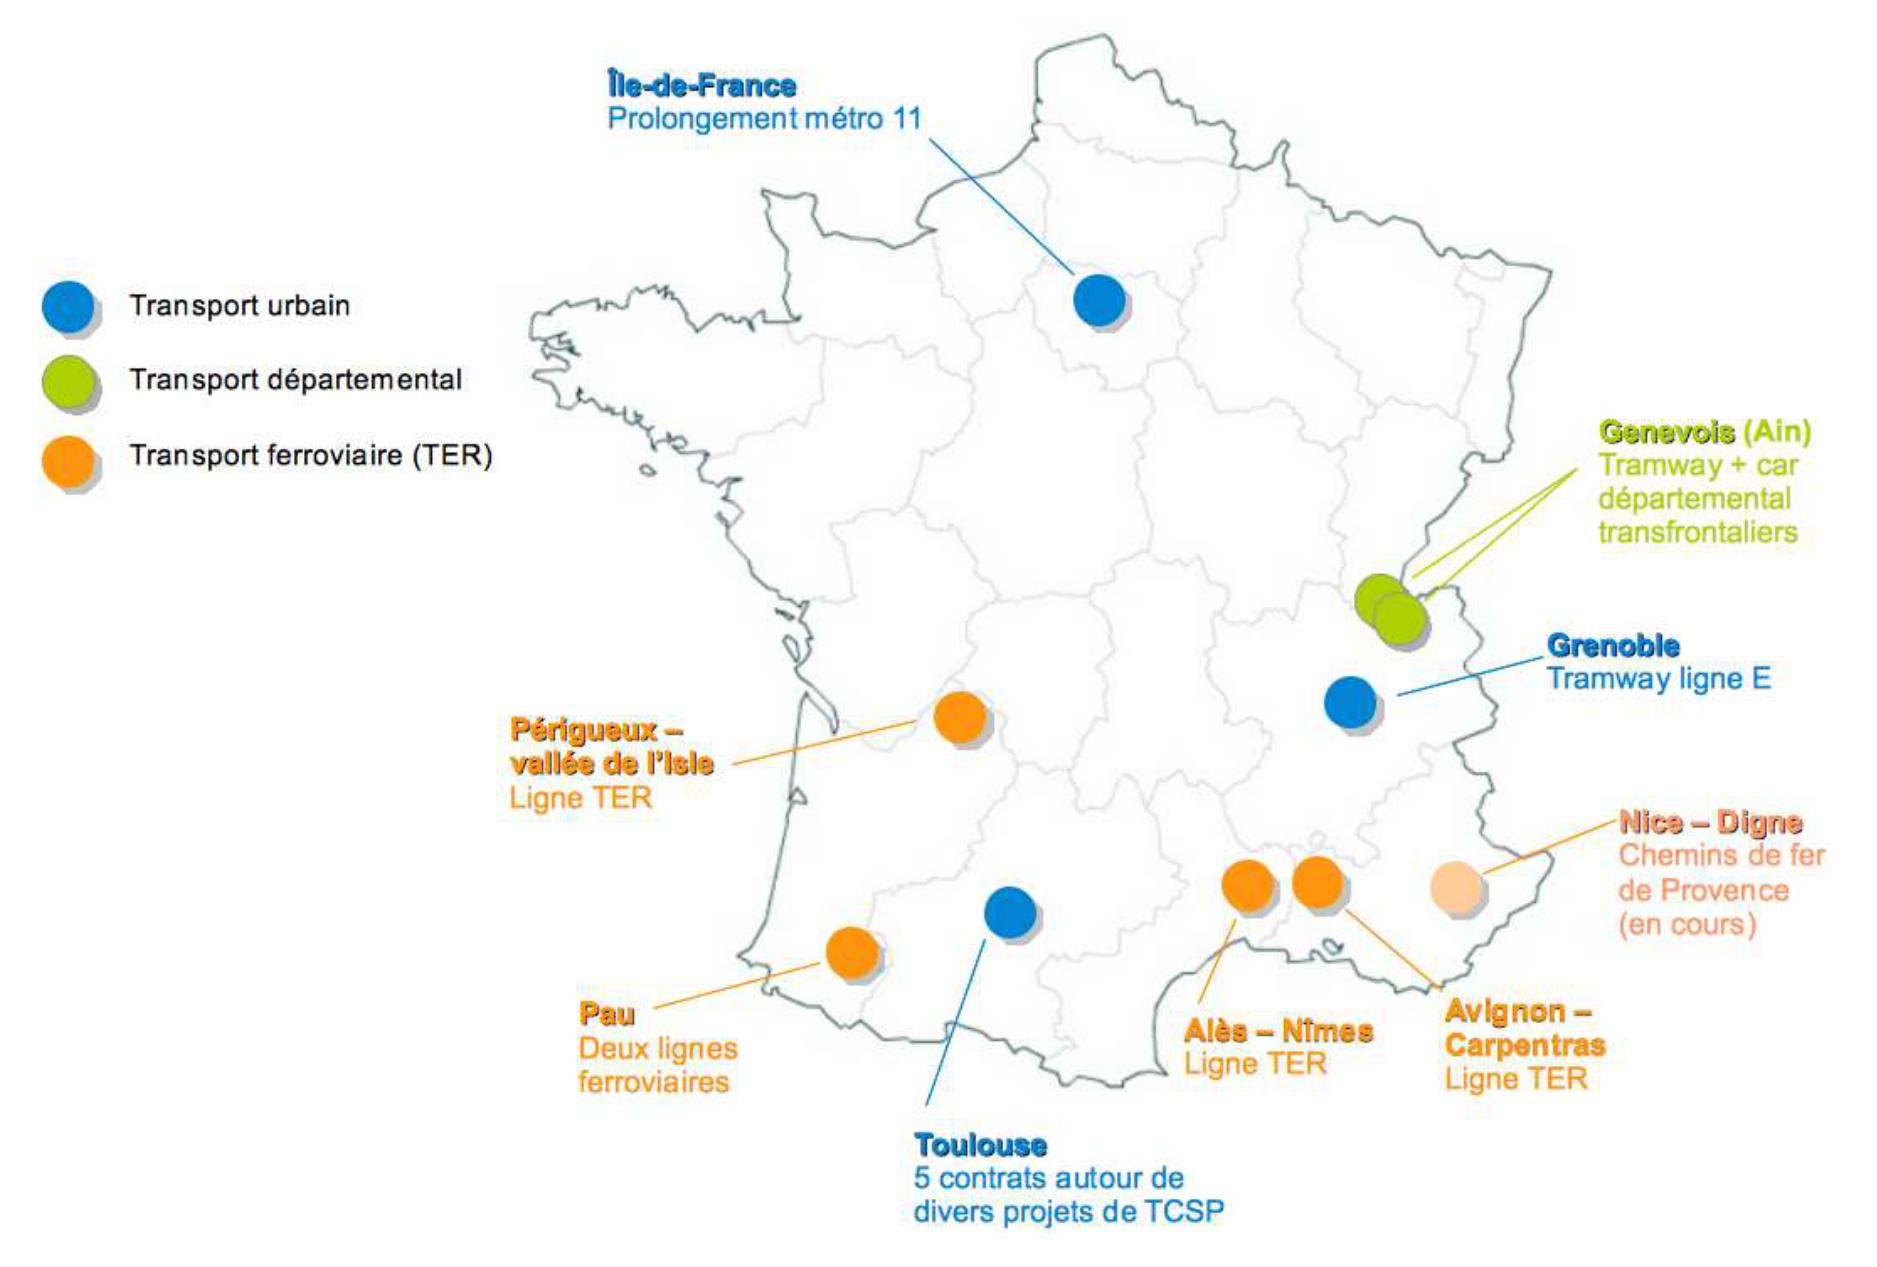
\includegraphics[width=0.75\columnwidth]{src/Figures/Chap-1/Carte_contrats_axe.jpg}}
        \vspace{5pt}
        \begin{flushright}\scriptsize{
        Source: \textcolor{blue}{\textcite[18]{bentayou_contrat_2015}}\index{Bentayou, Gilles|pagebf}\index{Perrin, Emmanuel|pagebf}\index{Richer, Cyprien|pagebf}
        }\end{flushright}
    \end{carte}

% Definition of contrats d'axe
In response to the recommendations made by \textcolor{blue}{\textcite[56]{lhostis_concevoir_2009}}\index{L'Hostis, Alain|pagebf}\index{Alexandre, Elsa|pagebf}\index{Appert, Manuel|pagebf}\index{Araud-Ruyant, Catherine|pagebf}\index{Basty, Marius|pagebf}\index{Biau, Géraldine|pagebf}\index{Bozzani-Franc, Sandra|pagebf}\index{Boutantin, Gratienne|pagebf}\index{Constantin, Chantal|pagebf}\index{Coralli, Monica|pagebf}\index{Durousset, Marie-Jeanne|pagebf}\index{Fradier, Christophe|pagebf}\index{Gabion, Cyrille|pagebf}\index{Leysens, Thomas|pagebf}\index{Mermoud, Françoise|pagebf}\index{Olny, Xavier|pagebf}\index{Perrin, Emmanuel|pagebf}\index{Robert, Jean|pagebf}\index{Simand, Noémie|pagebf}\index{Stransky, Vaclav|pagebf}\index{Soulas, Claude|pagebf}\index{Verdier, Anne-Marie|pagebf}\index{Vulturescu, Bogdan|pagebf} on the importance of creating a dialogue space dedicated to coordinating urban planning and transport\footnote{~
    In their French-German action-research report \textsl{Bahn.Ville 2}, \textcolor{blue}{\textcite[56]{lhostis_concevoir_2009}}\index{L'Hostis, Alain|pagebf}\index{Alexandre, Elsa|pagebf}\index{Appert, Manuel|pagebf}\index{Araud-Ruyant, Catherine|pagebf}\index{Basty, Marius|pagebf}\index{Biau, Géraldine|pagebf}\index{Bozzani-Franc, Sandra|pagebf}\index{Boutantin, Gratienne|pagebf}\index{Constantin, Chantal|pagebf}\index{Coralli, Monica|pagebf}\index{Durousset, Marie-Jeanne|pagebf}\index{Fradier, Christophe|pagebf}\index{Gabion, Cyrille|pagebf}\index{Leysens, Thomas|pagebf}\index{Mermoud, Françoise|pagebf}\index{Olny, Xavier|pagebf}\index{Perrin, Emmanuel|pagebf}\index{Robert, Jean|pagebf}\index{Simand, Noémie|pagebf}\index{Stransky, Vaclav|pagebf}\index{Soulas, Claude|pagebf}\index{Verdier, Anne-Marie|pagebf}\index{Vulturescu, Bogdan|pagebf} stress the importance of establishing a commission tasked with bringing together the relevant stakeholders and funding bodies, and developing the tools necessary for its proper functioning. In the fifth action of their report, the authors propose the creation of what they call the \Commas{Urban Planning and Mobility Interfaces Commission (IUD)}.
}, the \textsl{contrat d’axe} is a tool designed to strengthen the articulation between these two areas. The \textsl{contrat d’axe} thus represents an innovative instrument for territorializing the imperatives of this coordination, while illustrating a transformation of public action methods \textcolor{blue}{\autocite[427]{maulat_coordonner_2014}}\index{Maulat, Juliette|pagebf}\index{Beaucire, Francis|pagebf}. In practice, it is a negotiated approach between various partners aimed at defining clear partnership commitments within a framework inspired by the principles of \acrshort{TOD} \textcolor{blue}{\autocite[1]{cerema_outils_2021}}\index{Cerema@\textsl{Cerema}|pagebf}. The \textsl{contrat d’axe} promotes a logic of inter-territoriality, favoring cooperation between actors rather than hierarchy \textcolor{blue}{\autocite[112, 133]{vanier_pouvoir_2008}}\index{Vanier, Martin|pagebf}. This mechanism has a dual role: to create urban regulation and to align a territorial project within a contractual framework, without requiring the institutionalization of new levels of governance \textcolor{blue}{\autocite[11]{cerema_articuler_2010}}\index{Cerema@\textsl{Cerema}|pagebf}. Instead of mobilizing new resources, the \textsl{contrat d’axe} relies on the inventive reuse of available levers of action \textcolor{blue}{\autocite[12]{cerema_articuler_2010}}\index{Cerema@\textsl{Cerema}|pagebf}, seeking to synchronize the timelines between transport projects and urban developments \textcolor{blue}{\autocite[25]{meunier-chabert_contrats_2014}}\index{Meunier-Chabert, Martine|pagebf}. This approach marks an evolution in the design of railway projects, integrating them into a network-based territorial management logic and associating them with local planning projects \textcolor{blue}{\autocites[457, 468]{maulat_coordonner_2014}[94]{maulat_contractualiser_2015}}\index{Maulat, Juliette|pagebf}\index{Beaucire, Francis|pagebf}. Beyond its technical character, the \textsl{contrat d’axe} is a political tool aimed at strengthening the territorial foundation of regions and their position within the railway world \textcolor{blue}{\autocite[93]{maulat_contractualiser_2015}}\index{Maulat, Juliette|pagebf}.%%Translated%%

% Experiences with contrats d'axe
The experiences with \textsl{contrat d’axe} demonstrate a gradual \Commas{bottom-up} shift in practices, fostering new forms of cooperation and placing greater importance on local specificities and political negotiation \textcolor{blue}{\autocite[96]{maulat_contractualiser_2015}}\index{Maulat, Juliette|pagebf}. This generic tool allows for multiple adaptations depending on local contexts \textcolor{blue}{\autocite[457, 468]{maulat_coordonner_2014}}\index{Maulat, Juliette|pagebf}\index{Beaucire, Francis|pagebf}, mobilizing different sectors and scales, from tramway lines to railway ones \footnote{~
    Among the various forms of \textsl{contrats d’axe}, the railway contracts for \acrshort{TER} axes stand out due to their broader spatial scale, which requires the involvement of a larger number of partners \textcolor{blue}{\autocite[51]{cerema_articuler_2015}}. For regions, these contracts are a strategic tool to overcome the traditional \Commas{counter} logic in their relations with local authorities. They help improve communication on the costs and constraints related to railways while highlighting the actions taken in this regard \textcolor{blue}{\autocite[53]{cerema_articuler_2015}}. Moreover, they provide an opportunity to narrate railway and territorial policies \textcolor{blue}{\autocite{fandio_contrat_2023}}\index{Fandio, Cédric|pagebf}\index{Vezinaud, Nathan|pagebf}.
} \textcolor{blue}{\autocite[20]{afoun_mostaganem_2022}}\index{Afoun, Mohammed|pagebf}\index{Belguesmia, Noureddine|pagebf}. The approaches vary in terms of their degree of completion (see \hyperref[fig-chap1:carte-contrats-axe-france]{Map~\ref{fig-chap1:carte-contrats-axe-france}}, page~\pageref{fig-chap1:carte-contrats-axe-france}). For example, advanced contracts or charters have been implemented in Grenoble and Île-de-France, while initiatives are still in the preparatory stage in Lille and Geneva \textcolor{blue}{\autocites[2]{cerema_articuler_2010}[11]{cerema_articuler_2015}}\index{Cerema@\textsl{Cerema}|pagebf}. Whether in Toulouse, Grenoble, or Île-de-France, \textsl{contrats d'axe} have been integrated into the \acrfull{SCoT} and the \acrfull{SDRIF}. In the Occitan metropolitan area, the \acrfull{SCoT} introduced \Commas{urban-planning-transport coherence zones,} followed by \Commas{urban pacts,} aiming to intensify urbanization along existing or future corridors of major transport lines such as the metro, tramway, or \acrshort{BRT} \textsl{Linéo} \textcolor{blue}{\autocites[49]{toulouse_metropole_plui-h_2019}[26]{meunier-chabert_contrats_2014}[3]{cerema_outils_2021}}\index{Toulouse Métropole@\textsl{Toulouse Métropole}|pagebf}\index{Meunier-Chabert, Martine|pagebf}\index{Cerema@\textsl{Cerema}|pagebf}. In the Alpine agglomeration, the first \textsl{contrat d’axe} supports the commissioning of the tramway line E. This contract sets objectives for housing supply, public space requalification, and updates to the \acrfull{PLU} of the involved municipalities to incorporate urban intensification principles \textcolor{blue}{\autocites[3]{aurg_contrat_2022}[2]{cerema_outils_2021}}\index{AURG@\textsl{AURG}|pagebf}\index{Cerema@\textsl{Cerema}|pagebf}. The \Commas{territorial development contract} in Île-de-France, meanwhile, is part of the 2010 Grand Paris law framework. It supports the creation of new stations for the \textsl{Grand Paris Express} while facilitating their integration into regional planning projects \textcolor{blue}{\autocite[19]{cerema_articuler_2015}}\index{Cerema@\textsl{Cerema}|pagebf}. In the Lille metropolitan area, the \acrshort{DIVAT}\footnote{~
    Three main categories of \acrfull{DIVAT} have been identified, among the stops with more than ten daily crossings in each direction. Each category is associated with specific planning recommendations \textcolor{blue}{\autocite[23]{cerema_articuler_2010}}:
        \begin{customitemize}
    \item The \acrshort{DIVAT} of \Commas{level 1} includes the so-called \Commas{urban} \acrshort{TER} stops as well as metro and tram stations;
    \item The \acrshort{DIVAT} of \Commas{level 2} applies to \Commas{suburban} \acrshort{TER} stops and \Commas{urban} \acrshort{BRT} stations;
    \item The \acrshort{DIVAT} of \Commas{level 3} covers \Commas{suburban} \acrshort{TER} and \acrshort{BRT} stops.
        \end{customitemize}
    In 2010, 120 \acrshort{DIVAT} were listed, covering a third of the metropolitan population and a tenth of the total territory area \textcolor{blue}{\autocite[18]{cerema_articuler_2010}}. The \acrshort{DIVAT} aim to establish minimum density objectives for any new residential or commercial construction \textcolor{blue}{\autocite[19]{lmcu_plan_2011}}. They also specify parking standards, accessible pedestrian routes including accommodations for people with reduced mobility, and secure bike parking spaces installed every two to three metro or tram stations, in line with the cycling network \textcolor{blue}{\autocite[19]{lmcu_plan_2011}}.
}, integrated into the \acrfull{PLUi} and derived from the revision of the \acrshort{PDU}, define intervention areas within a 500-meter radius around \acrshort{TER} stations, metro, tram, and \acrshort{BRT} stations \textsl{Liane} \textcolor{blue}{\autocites[19]{lmcu_plan_2011}[26]{meunier-chabert_contrats_2014}}\index{Meunier-Chabert, Martine|pagebf}\index{Métropole Européenne de Lille@\textsl{Métropole Européenne de Lille}|pagebf}. Unlike the previous cases, this approach is managed by a unified authority, consolidating urban planning and transport competencies within the same administrative area \textcolor{blue}{\autocite[3]{cerema_articuler_2010}}\index{Cerema@\textsl{Cerema}|pagebf}.%%Translated%%

% Results and limitations
Due to their recent emergence, few studies have yet evaluated the outcomes of \textsl{contrats d’axe}, particularly those related to railways \textcolor{blue}{\autocite{fandio_contrat_2023}}\index{Fandio, Cédric|pagebf}\index{Vezinaud, Nathan|pagebf}. While most initiatives are still in development, these initial efforts can already be considered positive, according to \textcolor{blue}{\textcite[17-18]{cerema_articuler_2015}}\index{Cerema@\textsl{Cerema}|pagebf}. The contributions of the \textsl{contrats d’axe} manifest at several levels: the effective establishment of a dialogue and cross-disciplinary work space around transport corridors, overcoming administrative constraints; facilitating the development of transport projects; and achieving results in terms of guiding urbanization in line with transport services, with changes to urban planning rules and developments. A notable example is the Grenoble \textsl{contrat d’axe}, signed ten years ago, which achieved its goals: over 6,000 housing units were built along the strategic route, and the anticipated reduction in car traffic exceeded projections \textcolor{blue}{\autocites[7]{aurg_contrat_2022}[2]{cerema_outils_2021}}\index{AURG@\textsl{AURG}|pagebf}\index{Cerema@\textsl{Cerema}|pagebf}. Despite these encouraging results, several limitations still hinder the impact of \textsl{contrats d’axe}:
    \begin{customitemize}
\item \textsl{Institutional complexity and political orientation}. The \textsl{contrat d’axe} does not reduce the complexity related to the division of responsibilities between local authorities and decision-making levels, as demonstrated by \textcolor{blue}{Juliette} \textcolor{blue}{\textcite[469]{maulat_coordonner_2014}}\index{Maulat, Juliette|pagebf}\index{Beaucire, Francis|pagebf} in her doctoral thesis on the need for coordination between networks and territories in practice. It is more of a pragmatic tool for managing and regulating the gaps between institutional boundaries and territorial issues \textcolor{blue}{\autocite[96]{maulat_contractualiser_2015}}\index{Maulat, Juliette|pagebf}. While it opens up possibilities for better coordination, this instrument mainly functions as a governance and political communication tool, aimed at legitimizing a project \textcolor{blue}{\autocite[84]{gachon_impact_2019}}\index{Gachon, Mickaël|pagebf}. Unlike \acrshort{TOD}, which is more focused on technical programming and urban production, the \textsl{contrat d’axe} aims to reinvent a coordinated governance of transport and urban planning policies to address the dissociation of steering logics \textcolor{blue}{\autocites[118]{bentayou_contrat_2015}[20]{afoun_mostaganem_2022}}\index{Bentayou, Gilles|pagebf}\index{Perrin, Emmanuel|pagebf}\index{Richer, Cyprien|pagebf}\index{Afoun, Mohammed|pagebf}\index{Belguesmia, Noureddine|pagebf}. This approach thus requires significant investment in cross-disciplinary facilitation, typically managed by urban planning agencies \textcolor{blue}{\autocite[2]{cerema_outils_2021}}\index{Cerema@\textsl{Cerema}|pagebf};
\item \textsl{Non-binding nature}. These mechanisms have no legal standing in the \textsl{Urban Planning Code}, so the commitments made by the signatory partners are not subject to any legal obligations and do not have enforceable power \textcolor{blue}{\autocite[2]{cerema_outils_2021}}\index{Cerema@\textsl{Cerema}|pagebf}. Therefore, it is necessary to ensure that these commitments are reflected in prescriptive tools such as the \acrshort{PLU}, while fostering a collective dynamic of voluntary commitment. However, further exploration is needed to determine how this mechanism can be effectively integrated into existing operational planning tools, especially at the scale of micro-projects \textcolor{blue}{\autocite[53]{cerema_articuler_2015}}\index{Cerema@\textsl{Cerema}|pagebf}. Due to its limited scope, certain issues, often sensitive ones such as reducing car space, limiting urbanization in areas poorly served by public transport, or reorganizing rail services, are not addressed \textcolor{blue}{\autocite[96]{maulat_contractualiser_2015}}\index{Maulat, Juliette|pagebf}. These findings call for the design of a new generation of \textsl{contrats d’axe}, more binding on the urban aspect and focused on complex transformations, such as train-bike \gls{intermodality} \textcolor{blue}{\autocite[17]{haro_ligne_2021}}\index{Haro, Florent|pagebf}\index{Duvic, Nicolas|pagebf}. Furthermore, in the absence of a legal framework, there is a risk that these mechanisms remain limited to commitments of low scope, incapable of influencing the content or implementation methods of projects. On the contrary, they could become mere feasibility studies without a guarantee of implementation, turning into simple \textsl{gentlemen’s agreements} with no real enforceable power \textcolor{blue}{\autocite[53]{cerema_articuler_2015}}\index{Cerema@\textsl{Cerema}|pagebf};
\item \textsl{Continuity of methods}. The final limitation of \textsl{contrats d’axe} lies in the lack of renewal of practices. This project mechanism maintains sectoral logics and concentrates decision-making powers among public or parapublic actors, excluding \textsl{de facto} private stakeholders such as landowners, operators, or real estate developers \textcolor{blue}{\autocites[96]{maulat_contractualiser_2015}[2]{cerema_outils_2021}}\index{Maulat, Juliette|pagebf}\index{Cerema@\textsl{Cerema}|pagebf}. Unlike the more entrepreneurial \acrshort{TOD} common in the United States or Japan, the French \textsl{contrat d’axe} does not position itself as a \textsl{territorial marketing} tool aimed at attracting populations and investments to valued and competitive territories \textcolor{blue}{\autocite[120]{bentayou_contrat_2015}}\index{Bentayou, Gilles|pagebf}\index{Perrin, Emmanuel|pagebf}\index{Richer, Cyprien|pagebf}.%%Translated%%
    \end{customitemize}

% Transition
The incredible international diffusion capacity of \acrshort{TOD} is both a strength and a limitation of this planning concept, as it is by nature very composite and heterogeneous in its implementations \textcolor{blue}{\autocite[49]{bentayou_transit-oriented_2015}}\index{Bentayou, Gilles|pagebf}. In presenting this theoretical framework, we have chosen to outline the main model of its application in the French context, through the \textsl{contrats d’axe} that have been adopted and adapted. We could have focused on some international case studies of \acrshort{TOD} \textcolor{blue}{\autocite[6]{knowles_transports_2020}}\index{Knowles, Richard~D.|pagebf}\index{Ferbrache, Fiona|pagebf}\index{Nikitas, Alexandros|pagebf}, but we deliberately chose not to address them, given the many existing studies on the subject. These international examples, which reflect the diversity of \acrshort{TOD} adaptations since its formalization, will be discussed in more detail in the next section. We will then focus on recent developments and adaptations of this model, related to our research topic: the issue of \Commas{first and last miles,} and in particular the solutions provided by bicycles, in connection with train stations and their urban environment, to address the shortcomings of car-centered systems.%%Translated%%

% 1.1.3.2.
\needspace{1\baselineskip} % Reserve space
\subsubsection*{Main Adaptations and Renewal of \textsl{Transit-Oriented Development}
    \label{chap1:tod-presentation-generale-declinaisons-hybrids}
    }

    % Introduction Transit Metropolises
In this final subsection, which serves as a transition to the introduction of bicycles and their close relationship with \acrshort{TOD}, we aim to trace the evolution of what mobility and urbanism expert and consultant \textcolor{blue}{Robert} \textcolor{blue}{\textcite[11]{cervero_transit_1998}}\index{Cervero, Robert|pagebf}, in his book \foreignlanguage{english}{\textsl{Transit Metropolis: A Global Inquiry}}, refers to as the concept of \Commas{\textsl{Transit Metropolises}}. These territories, characterized by metropolitanization structured around public transport networks, indeed represent the practical implementation of \acrshort{TOD} principles, often predating its conceptual formalization. They are metropolitan areas that have successfully combined urban forms and mobility systems \textcolor{blue}{\autocite[132]{cervero_transit_2020}}\index{Cervero, Robert|pagebf}. This typology of \Commas{success stories} illustrates, in a deductive manner, how these territories have simultaneously adopted and influenced the adaptable directions of \acrshort{TOD} \textcolor{blue}{\autocite[134]{wheeler_transit_2000}}\index{Wheeler, Stephen~M.|pagebf}. To do so, the author identifies four major adaptations of this planning concept on a global scale: \Commas{adaptive cities}, \textsl{Adaptive Cities}, \Commas{adaptive public transport networks}, \textsl{Adaptive Transit}, \Commas{strong-core cities}, \textsl{Strong-core cities}, and \Commas{hybrid models}, \textsl{Hybrids}, which highlight the inventive ways in which \acrshort{TOD} policies materialize depending on the urban legacies specific to each local context.%%Translated%%

% 1 : Adaptive Cities
First, \textsl{Adaptive Cities} have relied, or continue to rely, on the early development of public transport services that condition the structuring of dense and mixed territories to control urban growth. By anticipating this growth at the metropolitan scale, the goal is to preserve a \Commas{green belt} while organizing movement flows through compact, multifunctional satellite cities that are interconnected with the main urban centers (see \hyperref[fig-chap1:schema-transit-metropolis]{Map~\ref{fig-chap1:schema-transit-metropolis}}, page~\pageref{fig-chap1:schema-transit-metropolis}). This specific form of \textsl{Transit Metropolis} relies on a long-term vision, supported by a high-performance and structuring public transport system \textcolor{blue}{\autocite[132]{cervero_transit_1998}}\index{Cervero, Robert|pagebf}. Several \textsl{Adaptive Cities} are recognized as models of best practices related to \acrshort{TOD}. Among them, we can mention the urban growth model of Stockholm's satellite cities from 1945\footnote{~
    Thanks to significant public land reserves, the Swedish capital chose to develop a network of satellite cities to control urban growth, while offering a polycentric metropolitan system \textcolor{blue}{\autocite[p.~109-130 (Chapter~4)]{cervero_transit_1998}}\index{Cervero, Robert|pagebf}. This project envisions Stockholm in the shape of a star, metaphorically described as a \Commas{pearls on a necklace,} connecting satellite communities radially to the urban center via the \textsl{Tunnelbana} metro system \textcolor{blue}{\autocite[111]{pojani_past_2018}}\index{Pojani, Dorina|pagebf}\index{Stead, Dominic|pagebf}\index{Shiftan, Yoram|pagebf}\index{Kamargianni, Maria|pagebf}. The General Plan developed between 1945 and 1952 notably foresaw the commissioning of four, then eight \textsl{Tunnelbana} lines, electrified and with high service frequency \textcolor{blue}{\autocite[4]{knowles_transports_2020}}\index{Knowles, Richard~D.|pagebf}\index{Ferbrache, Fiona|pagebf}\index{Nikitas, Alexandros|pagebf}. Between these satellite cities, preserved natural and agricultural spaces can be found \textcolor{blue}{\autocite[1-63]{strong_planned_1971}}\index{Strong, Ann Louise|pagebf}. The first generation of satellite cities includes emblematic locations such as Vällingby, an internationally recognized prototype \textcolor{blue}{\autocite[23]{gullberg_city-building_2004}}\index{Gullberg, Anders|pagebf}\index{Kaijser, Anne|pagebf}, as well as Farsta, Skärholmen, Järva, and Täby, developed between the 1950s and 1970s. The resulting urban planning relies on the policy called \textsl{Arbete, Bostad, Centrum} (\textsl{ABC-stad}), which aims to integrate the economic and administrative sectors near train stations within pedestrian spaces. Housing, predominantly family-oriented, is located less than one kilometer from the stations \textcolor{blue}{\autocite[112]{pojani_past_2018}}\index{Pojani, Dorina|pagebf}\index{Stead, Dominic|pagebf}\index{Shiftan, Yoram|pagebf}\index{Kamargianni, Maria|pagebf}. This strategy, supported by financial incentives, aims to avoid the formation of \Commas{bedroom suburbs} and ensure efficient flow organization, particularly through bidirectional commuter traffic \textcolor{blue}{\autocites[43]{cervero_sustainable_1995}[22]{gullberg_city-building_2004}}\index{Cervero, Robert|pagebf}\index{Gullberg, Anders|pagebf}\index{Kaijser, Anne|pagebf}. The results of this approach were quickly evident: between 1980 and 1990, Stockholm was the only one of 37 cities worldwide to record a decrease in the modal share of cars. During peak hours, 55\% of commuters travel in one direction, while 45\% travel in the opposite direction, demonstrating the efficiency of the system \textcolor{blue}{\autocites[705]{kenworthy_patterns_1999}[24]{curtis_transit_2009}}\index{Curtis, Carey|pagebf}\index{Renne, John Luciano|pagebf}\index{Bertolini, Luca|pagebf}\index{Kenworthy, Jeffrey~R.|pagebf}\index{Laube, Felix~B.|pagebf}.
}; the \textsl{Finger Plan} of Copenhagen in 1947\footnote{~
    In a similar context to Stockholm after the war, the Danish capital developed a master plan in 1947. This project, supported by a group of architects and urban planners \textcolor{blue}{\autocite[p.~132-153 (Chapter~5)]{cervero_transit_1998}}\index{Cervero, Robert|pagebf}, aimed to consolidate five railway corridors, illustrated by the metaphor of the \textsl{Finger Plan} (\textsl{Egnsplan}) \textcolor{blue}{\autocite[123-128]{teknisk_kontor_for_udvalget_til_planlaegning_af_kobenhavnsegnen_skitseforslag_1947}}\index{Teknisk kontor for udvalget til planlægning af Københavnsegnen@\textsl{Teknisk kontor for udvalget til planlægning af Københavnsegnen}|pagebf}. These five fingers, representing the railway corridors, allow radial connection of over 29 municipalities to the urban center of the metropolis \textcolor{blue}{\autocite[]{fullerton_scandinavia_1991}}\index{Fullerton, Brian|pagebf}\index{Knowles, Richard~D.|pagebf}, marked by the constraint of limited land in the city \textcolor{blue}{\autocites[254]{knowles_transit_2012}[4-6]{the_danish_nature_agency_finger_2015}}\index{Knowles, Richard~D.|pagebf}\index{The Danish Nature Agency@\textsl{The Danish Nature Agency}|pagebf}. Since the adoption of the \textsl{Master Plan} in 1989, urbanization has been strictly limited to a one-kilometer perimeter along the \Commas{fingers.} This measure has preserved the agricultural and natural spaces located between the different corridors \textcolor{blue}{\autocite[224]{vuk_transport_2005}}\index{Vuk, Goran|pagebf}. In the 1990s and 2000s, the project underwent a shift marked by the construction of a sixth \Commas{finger,} introducing a break with the original polycentric model. This new corridor allowed the development of the new city of Ørestad, connected to the metro, in a bid for global competitiveness. However, this shift, part of a more neoliberal agenda, did not challenge the application of \acrshort{TOD} principles in Copenhagen \textcolor{blue}{\autocites[103-105]{majoor_progressive_2008}[254]{knowles_transit_2012}}\index{Knowles, Richard~D.|pagebf}\index{Majoor, Stan|pagebf}.
}; the \textsl{Concept Plan} of Singapore in 1971\footnote{~
    Starting in 1965, when it gained full sovereignty, the city-state of Singapore embarked on an ambitious urban planning project based on a master plan \textcolor{blue}{\autocite[p.~155-179 (Chapter~6)]{cervero_transit_1998}}\index{Cervero, Robert|pagebf}, initially called the \textsl{Ring Plan}. The national housing development agency, the \acrfull{HDB}, began constructing over 600,000 public housing units, most of which were intended for sale \textcolor{blue}{\autocite[167]{guillot_singapour_2007}}\index{Guillot, Xavier|pagebf}. However, it was in 1971, with the revision of the \textsl{Long Range Concept Plan}, that Singapore truly began implementing, over two decades, a public transport-oriented development matrix. The plan includes the construction of a dense network of \acrfull{MRT}, Singapore's metro (\textsl{Sistem Pengangkutan Gerak Cepat}), serving twenty new high-density cities \textcolor{blue}{\autocite[162]{cervero_transit_1998}}\index{Cervero, Robert|pagebf}. The last stage of Singapore's urban planning took place in 1991, with the ratification of the \textsl{Revised Concept Plan}, marked by the ambition to create a \Commas{\textsl{Tropical City of Excellence}}. This plan introduced greater private sector participation in housing development \textcolor{blue}{\autocite[168]{guillot_singapour_2007}}\index{Guillot, Xavier|pagebf}. In this framework, the \textsl{Constellation Plan} was developed, aiming to relocate commercial establishments near \acrshort{MRT} stations \textcolor{blue}{\autocite[362]{richmond_transporting_2008}}\index{Richmond, Jonathan~E.~D.|pagebf}. This urban development is accompanied by strict national policies regulating car ownership and usage. These measures include a quota system to limit the number of vehicles allowed on the road (\textsl{Vehicle Quota Scheme}), as well as disincentive taxes on car ownership. Furthermore, the \textsl{Electronic Road Pricing} system imposes significant charges for the use of road infrastructure and parking \textcolor{blue}{\autocite[162]{joshi_transit-oriented_2017}}\index{Joshi, Rutul|pagebf}\index{Yogi, Joseph|pagebf}\index{Patel, Kavina|pagebf}\index{Darji, Vishal|pagebf}.
}; or the \textsl{Tokyu Method} in Tokyo since at least the interwar period\footnote{~
    The Tokyo approach lies less in the definition of \textsl{Master Plans} than in an entrepreneurial logic driven jointly by the private and public sectors since the late 1920s \textcolor{blue}{\autocite[p.~181-209 (chapter 7)]{cervero_transit_1998}}\index{Cervero, Robert|pagebf}. Although Tokyo is not the only metropolis to have adopted this strategy \textcolor{blue}{\autocite[87]{bertolini_developing_2016}}\index{Bertolini, Luca|pagebf}\index{Chorus, Paul|pagebf}, it developed a unique approach known as \textsl{conglomerate Transit-Oriented Development}, reinforced by the urban growth of the metropolis between 1945 and 1982 \textcolor{blue}{\autocite[28-29]{liu_historical_2024}}\index{Liu, Yudi|pagebf}\index{Manabe, Rikutaro|pagebf}\index{Nitanai, Ryoichi|pagebf}\index{Murayama, Akito|pagebf}. The development of public transport was actively supported by massive private sector investments, with the emblematic example of \textsl{Tokyu Corporation}. Since the early 20\textsuperscript{th} century, this company began acquiring vast land areas in the metropolis with the aim of developing urban projects centered around the railway lines it operated. This strategy, known as the \textsl{Tokyu Method}, is based on capturing land value appreciation by purchasing land before the construction of railway infrastructure. It illustrates an entrepreneurial approach to \acrshort{TOD}, based on a \Commas{win-win} partnership: public authorities play a coordination role, while transport operators ensure profitability not only through passenger fares but also through land speculation. By 2004, the \textsl{Tokyu Corporation} derived only 41\% of its net income from passenger transport, with the rest generated by activities related to land rent and leasing land for housing, commerce, and hotels \textcolor{blue}{\autocite[110]{suzuki_financing_2015}}\index{Suzuki, Hiroaki|pagebf}. This approach contributed to the transformation of urban forms, shifting from a centralized organization to a highly decentralized model. The resulting multimodal neighborhoods allow for significant decongestion of the urban core, once dominated by the old main station of Tokyo \textcolor{blue}{\autocite[29]{liu_historical_2024}}\index{Liu, Yudi|pagebf}\index{Manabe, Rikutaro|pagebf}\index{Nitanai, Ryoichi|pagebf}\index{Murayama, Akito|pagebf}.
} \textcolor{blue}{\autocite[109-209]{cervero_transit_1998}}\index{Cervero, Robert|pagebf}. Further research will enrich this category by adding new examples, including European ones, such as those of Amsterdam and Rome examined in the doctoral thesis of \textcolor{blue}{Merijn} \textcolor{blue}{\textcite[180-206]{martens_adaptive_2006}}\index{Martens, Merijn|pagebf}, as well as those of Paris and Hong Kong \textcolor{blue}{\autocite[4]{knowles_transports_2020}}\index{Knowles, Richard~D.|pagebf}\index{Ferbrache, Fiona|pagebf}\index{Nikitas, Alexandros|pagebf}.%%Translated%%

% Figure Transit Metropolises
\begin{carte}[h!]\vspace*{4pt}
    \caption{Abstract maps of updated \textsl{Transit Metropolises}.}
    \label{fig-chap1:schema-transit-metropolis}
    \centerline{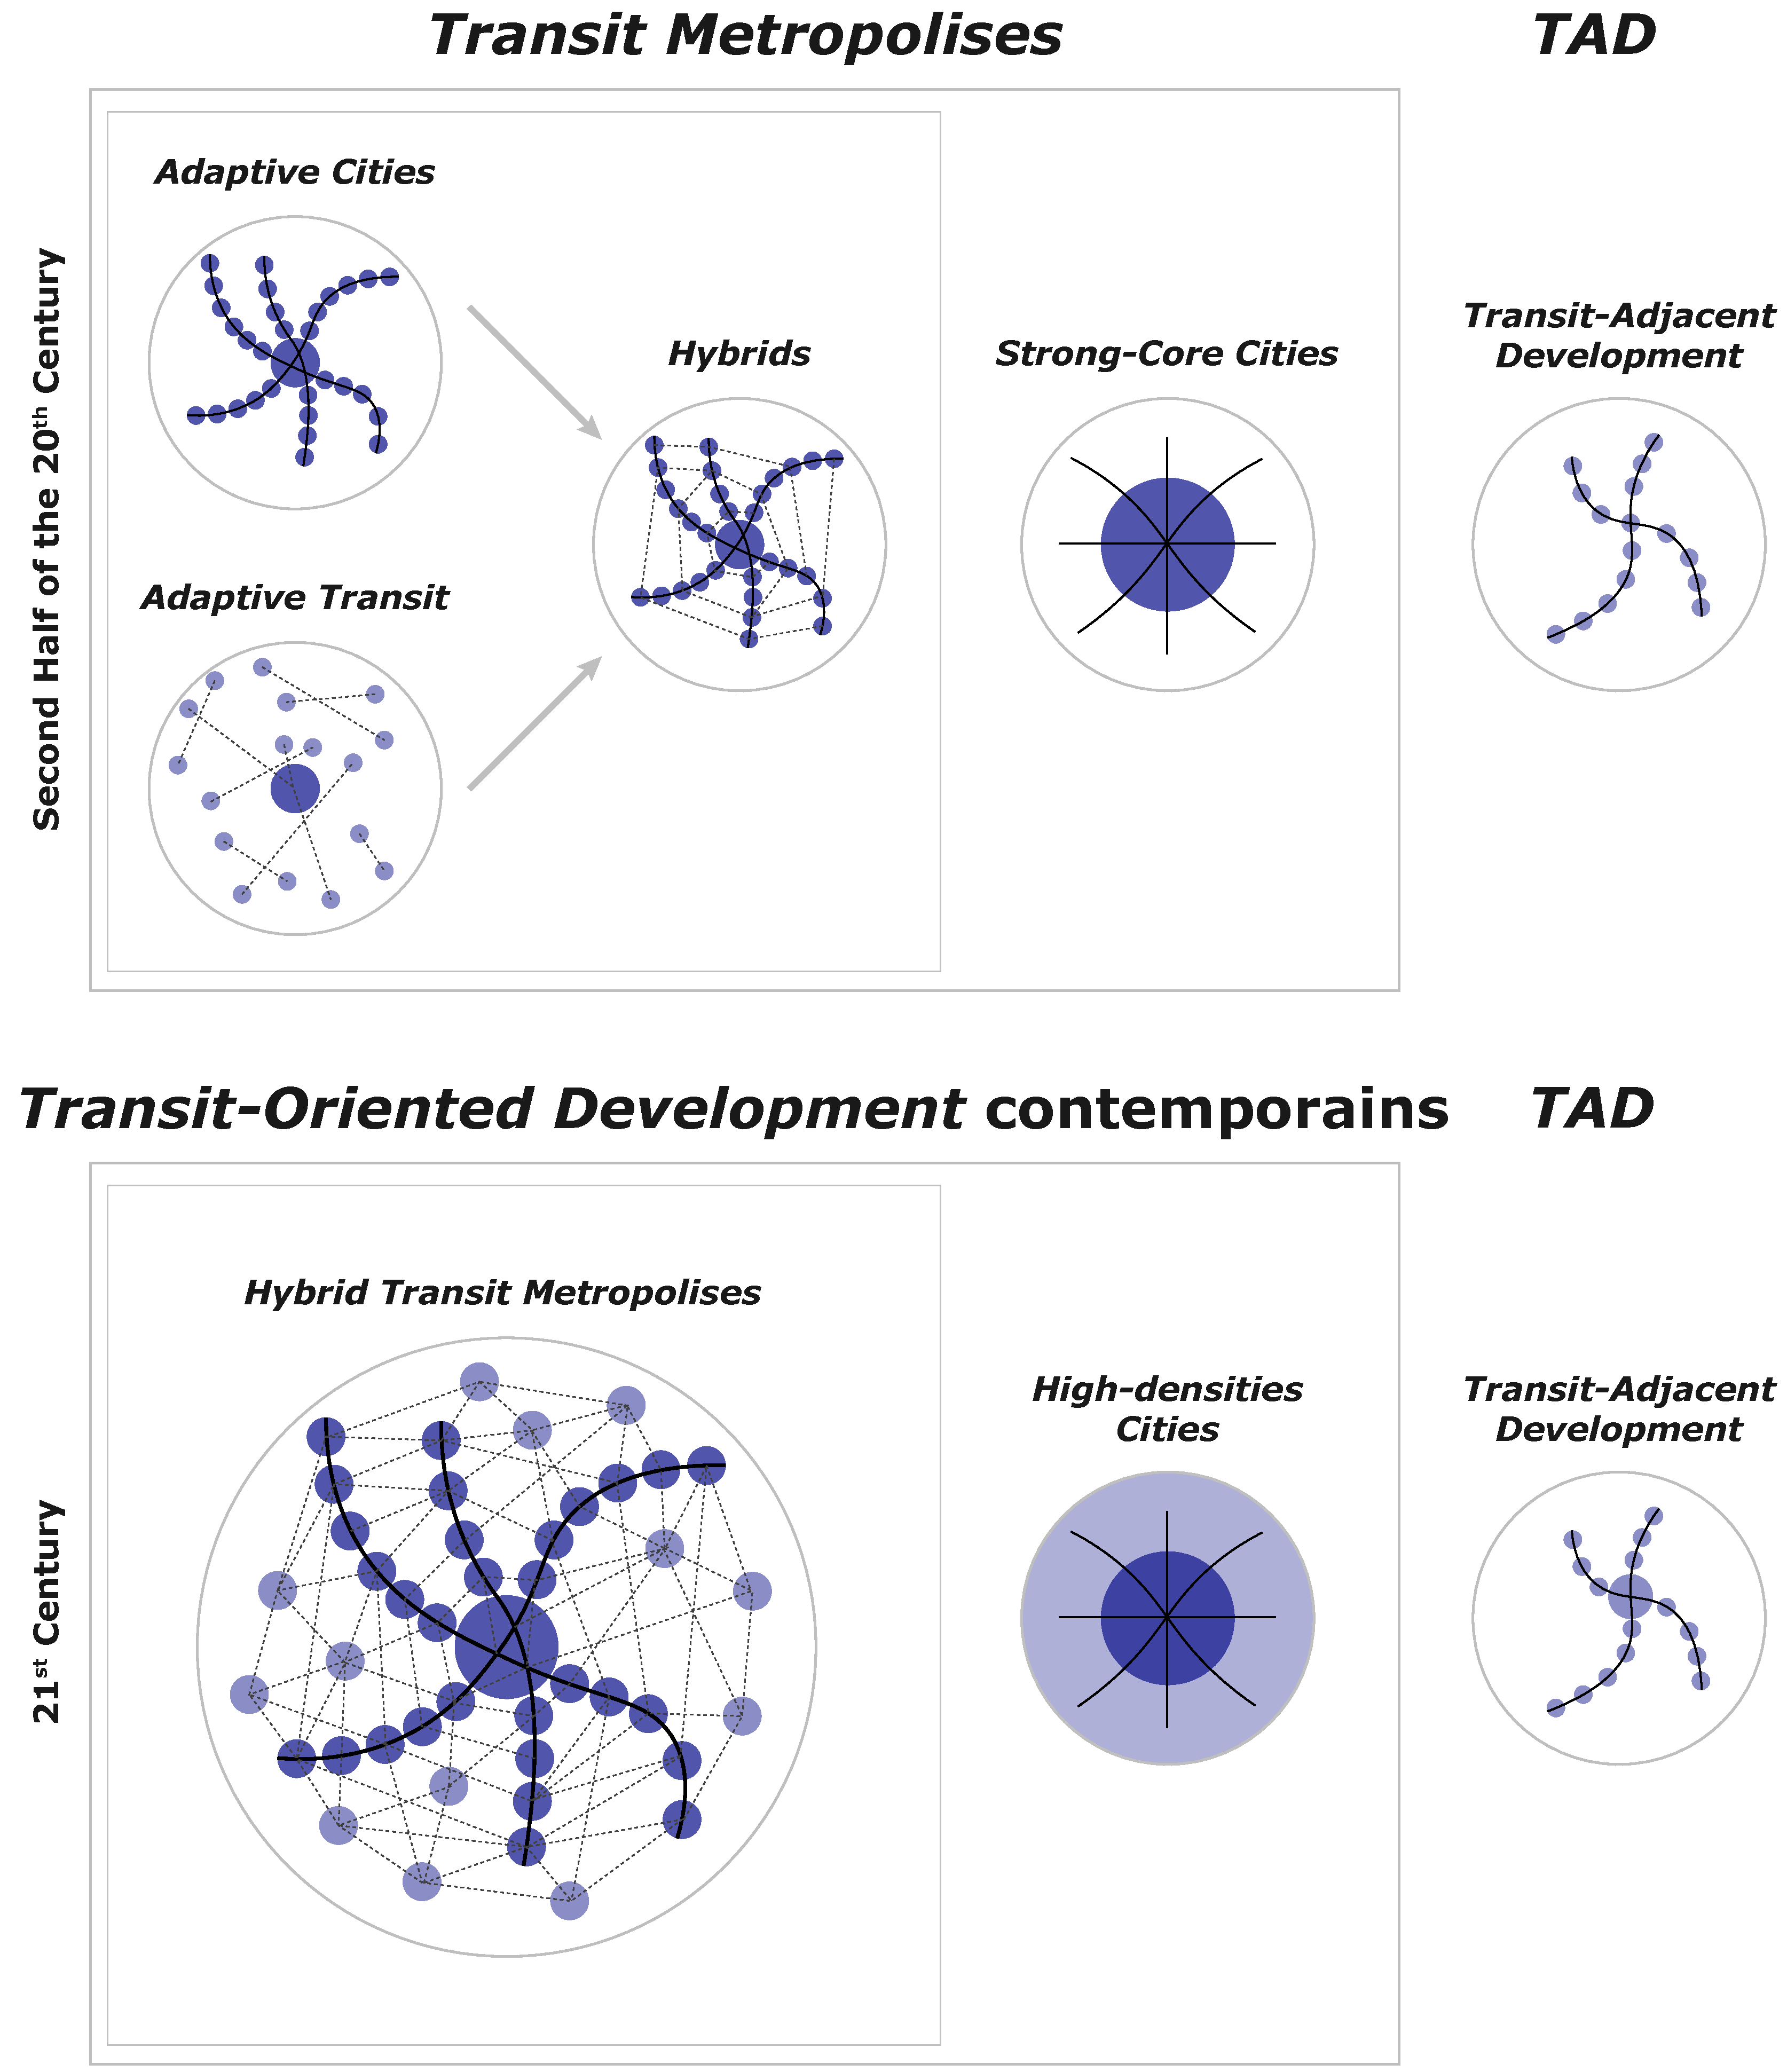
\includegraphics[width=1\columnwidth]{src/Figures/Chap-1/EN_Schema_Alternative_cities_transit.pdf}}
    \vspace{5pt}
    \begin{flushright}\scriptsize{
    Sources: \textcolor{blue}{\textcite[3]{vos_influence_2014}}\index{Vos, Jonas de|pagebf}\index{Acker, Veronique van|pagebf}\index{Witlox, Frank|pagebf} and \textcolor{blue}{\textcite[2]{liu_historical_2024}}\index{Liu, Yudi|pagebf}\index{Manabe, Rikutaro|pagebf}\index{Nitanai, Ryoichi|pagebf}\index{Murayama, Akito|pagebf}
    \\
    Graphic adaptation: \textcolor{blue}{Dylan Moinse (2025)}
    }\end{flushright}
\end{carte}

% Adaptive Transit
\textsl{Adaptive Transit}, characterized by more pronounced urban sprawl, has chosen to reverse the reasoning between urban growth and transport networks. To effectively serve low-density peri-urban areas, mobility systems must adapt to the dispersed urban forms of these spaces. \textcolor{blue}{Susan} \textcolor{blue}{\textcite[108]{handy_reviews_1999}}\index{Handy, Susan|pagebf} highlights this issue, arguing that U.S. cities, heavily marked by urban sprawl, cannot directly replicate the experiences of \textsl{Adaptive Cities} and must instead adopt a model based on \textsl{Adaptive Transit}. In these urban contexts, regional movement follows tangent flows rather than radial ones, connecting the suburbs to each other (see \hyperref[fig-chap1:schema-transit-metropolis]{Map~\ref{fig-chap1:schema-transit-metropolis}}, page~\pageref{fig-chap1:schema-transit-metropolis}). However, conventional public transport networks are often organized around fixed, radial, or sometimes diametrical routes, limiting their capacity to meet these needs. The solutions proposed by this type of \textsl{Transit Metropolis}, also known by the acronym \acrfull{DOT}, rely on technological and service innovations to offer greater flexibility, capable of competing with the private car \textcolor{blue}{\autocite[132]{cervero_transit_2020}}\index{Cervero, Robert|pagebf}. The goal of these systems is to promote alternative mobility to the car-centric model while providing transport services with characteristics similar to those of the car \textcolor{blue}{\autocite[67-68]{bourdin_major_2024}}\index{Bourdin, Alain|pagebf}. These solutions focus on personalized routes, adapted to the challenges of the \Commas{first and last miles} as well as \Commas{door-to-door} mobility needs. These demand-based services complement traditional public transport by enhancing their attractiveness and accessibility. \textsl{Adaptive Transit} can be illustrated by the tram-train system in Karlsruhe, launched in 1992\footnote{~
    Confronted with significant peri-urbanization and a lack of coordination between public transport agencies, the city of Karlsruhe initially struggled to optimize its urban transport network \textcolor{blue}{\autocite[p.~343-360 (Chapter~13)]{cervero_transit_1998}}\index{Cervero, Robert|pagebf}. To address this issue, a context-appropriate project was developed: the design of an interconnected tram-train system, known as the \textsl{Zweisystem-Stadtbahn}. The first line of this system serves the downtown area of Karlsruhe in tram mode, then uses interurban railway tracks to reach Bretten. This project, tested in 1986 before its official launch in 1992, aims to offer an effective solution for peri-urban mobility needs. The commissioning of this pilot line, which quickly saw its frequency increase, achieved its objectives, including a fourfold increase in ridership, mostly former car users \textcolor{blue}{\autocite[41]{beaucire_reseau_2000}}\index{Beaucire, Francis|pagebf}. Beyond its technical aspects, the \Commas{Karlsruhe model} today garners significant interest \textcolor{blue}{\autocite[41]{beaucire_reseau_2000}}\index{Beaucire, Francis|pagebf}. This system provides an effective response to a heterogeneous urban context by efficiently connecting peri-urban areas that had not been integrated into the public transport network before \textcolor{blue}{\autocite[57-65]{grisot_manifeste_2020}}\index{Grisot, Sylvain|pagebf}. This unique technical and fare system allows residents of peri-urban areas to directly reach urban centers without needing to transfer, thus bypassing often remote train stations. At the same time, for local governments and transport operators, this model represents a promise of lower-cost investment through the reuse of existing infrastructure \textcolor{blue}{\autocite[17]{lhostis_multi-criteria_2017}}\index{L'Hostis, Alain|pagebf}\index{Soulas, Claude|pagebf}\index{Vulturescu, Bogdan|pagebf}.
}; the guided bus system in Adelaide, fully operational since 1989\footnote{~
    The city of Adelaide faces a situation similar to Karlsruhe, marked by considerable urban expansion \textcolor{blue}{\autocite[p.~362-377 (Chapter~14)]{cervero_transit_1998}}\index{Cervero, Robert|pagebf}. In response to the rapid urban growth of suburbs to the northeast of the metropolitan area, public authorities initially chose to extend the existing tram network, before turning to an alternative solution: the implementation of a guided bus system. This system, known as the \textsl{O-Bahn}, was the first of its kind in the world and remains the longest network in service today. It constitutes a hybrid between conventional buses and rail transport \textcolor{blue}{\autocite[143]{currie_assessing_2014}}\index{Currie, Graham|pagebf}\index{Delbosc, Alexa|pagebf}. The \textsl{O-Bahn} relies on the use of specific lateral wheels, allowing the \acrshort{BRT} to travel on dedicated, off-road lanes, making the journey both faster and safer \textcolor{blue}{\autocite[2]{currie_bus_2006}}\index{Currie, Graham|pagebf}. This system is designed to efficiently connect the city's \acrfull{CBD} to the new commercial and urban hub of Tea Tree Plaza, located in a rapidly expanding suburb. When it was launched, the \textsl{O-Bahn} had 6 kilometers of tracks in 1986, which were extended to 12 kilometers in 1989. The primary goal was to relieve congestion on the highway network by offering a high-performance, flexible, and relatively low-cost service. The \textsl{O-Bahn} network thus achieves an average commercial speed of 80 kilometers per hour, making it the fastest bus system in the world \textcolor{blue}{\autocite[3]{currie_bus_2006}}\index{Currie, Graham|pagebf}. This success can be attributed to the dedicated infrastructure and the long distance between stops, about five kilometers. Additionally, the occupancy rate of the guided buses is generally twice that of the regular buses in the metropolitan area, while the operating costs per passenger per kilometer are a third lower than those of regular buses \textcolor{blue}{\autocite[7]{basbas_advances_2005}}\index{Basbas, Socrates|pagebf}. Currently, 18 lines use the 12-kilometer alignment, although only 8 of them operate it in its entirety \textcolor{blue}{\autocite[3]{rogers_o-bahn_2002}}\index{Rogers, Lee~H.|pagebf}. This system illustrates how a region faced with significant peri-urbanization chose not to contain this urban dynamic but to connect it to the urban core. The \textsl{O-Bahn} infrastructure is also able to cross dense neighborhoods without requiring significant space reconfigurations. However, despite the system's popular and even tourist success, Adelaide remains dominated by cars. This dominance is also reflected among \textsl{O-Bahn} users, over half of whom drive to the stations, necessitating recurrent expansion of \acrfull{PnR} facilities. These expansions occur despite initial efforts to improve pedestrian and cycling infrastructure around the stations \textcolor{blue}{\autocite[11]{currie_bus_2006}}\index{Currie, Graham|pagebf}.
}; or the \textsl{paratransit} system, called \textsl{microbús}, in Mexico City\footnote{~
    In Mexico City, the significant gap between public transport provision and the extent of the urbanized area has fostered the emergence of self-regulated strategies initiated by the market. It was in this context that the private transport service \textsl{microbús}, also known as \textsl{pesero}, was established in the 1970s. This system developed spontaneously to meet mobility needs in areas not served by the public transport network \textcolor{blue}{\autocite[p.~379-399 (Chapter~15)]{cervero_transit_1998}}\index{Cervero, Robert|pagebf}. Thus, the market adapted to bridge the gap between growing mobility demand and insufficient infrastructure and service provision. Faced with the rapid expansion of Mexico City's urban area, \textsl{paratransit} found its place within the mobility system by coexisting as a transfer mode. This service enables the transportation of isolated populations to public transport stations located on the outskirts of the city center. Operating like collective taxis, these vehicles, often originally cars, follow a fixed route similar to that of a bus line. They pick up and drop off passengers on demand along the \gls{itinerary} \textcolor{blue}{\autocite[4]{chiu_does_2022}}\index{Chiu, Bing-yu|pagebf}. This \Commas{informal} system plays a key role as a self-organized feeder service, as confirmed by the existing literature \textcolor{blue}{\autocite[98, 246]{adjeroud_coexistence_2024}}\index{Adjeroud, Heythem|pagebf}\index{Chapelon, Laurent|pagebf}\index{Lammoglia, Adrien|pagebf}. It notably has the advantage of not necessarily requiring public investment. However, it can represent direct competition to formal public transport and can contribute to urban sprawl \textcolor{blue}{\autocite[4]{chiu_does_2022}}\index{Chiu, Bing-yu|pagebf}. Based on this, \textcolor{blue}{Edzani} \textcolor{blue}{\textcite[65]{libunyu_paratransit-oriented_2024}}\index{Libunyu, Edzani|pagebf} identifies a form of \textsl{Paratransit-Oriented Transit-Oriented Development}, using Mexico City as an example.
} \textcolor{blue}{\autocite[343-399]{cervero_transit_1998}}\index{Cervero, Robert|pagebf}.%%Translated%%

% Hybrids
Deliberately leaving aside the \textsl{Strong-core Cities}, which are based on urban revitalization dynamics and are somewhat distant from our central issue, we focus on the fourth and final type of \textsl{Transit Metropolis}: the \textsl{Hybrids}, which hold particular relevance for our research. Going beyond the dichotomy between \textsl{Adaptive Cities} and \textsl{Adaptive Transit}, these \textsl{Hybrids} stand out by their ability to leverage the strengths of both concepts. This approach seeks to find a balance between dense and mixed urbanism concentrated along well-served corridors and an efficient alternative mobility system designed to cover low-density peripheries. This compromise is illustrated by \hyperref[fig-chap1:schema-transit-metropolis]{Map~\ref{fig-chap1:schema-transit-metropolis}} (page~\pageref{fig-chap1:schema-transit-metropolis}). These \textsl{Hybrids} combine, within a single territory, the mobility and urbanism solutions derived from the two types of \textsl{Transit Metropolis} described earlier. They thus align with a polycentric model, characterized by a hierarchy of interconnected urban centers linked by structuring lines. The accessibility of these centers is enhanced by flexible mobility services that meet the needs of peri-urban and low-density areas \textcolor{blue}{\autocite[213-295]{cervero_transit_1998}}\index{Cervero, Robert|pagebf}.%%Translated

% Hybrid Transit Metropolises
This typology of \textsl{Transit Metropolises}, \textcolor{blue}{Robert} \textcolor{blue}{\textcite[131]{cervero_transit_2020}}\index{Cervero, Robert|pagebf} ultimately reinterprets it under the consolidated designation of \textsl{Hybrid Transit Metropolises}. Such a reinterpretation highlights how these territories have transcended the dichotomy between \textsl{Adaptive Cities} and \textsl{Adaptive Transit}, a duality that has now lost its relevance. This observation refers to the \textsl{Hybrids}, as described by \textcolor{blue}{\textcite[213-295]{cervero_transit_1998}}\index{Cervero, Robert|pagebf} twenty years earlier, although revisited in light of contemporary developments in mobility systems. The determining factor in this revision lies in the emergence and generalization of \acrshort{ICT}, which have simultaneously led to \Commas{smart mobility} and \Commas{smart cities.} Furthermore, the mobility practices and imaginaries of new generations have significantly evolved, influencing travel patterns and accessibility expectations. Behind these concepts, sometimes referred to as \Commas{buzzwords,} \textcolor{blue}{\textcite[137-143]{cervero_transit_2020}}\index{Cervero, Robert|pagebf} advocates for an integrative approach, surpassing the divides in favor of \textsl{Transit Metropolises of the 21\textsuperscript{st} century}. At the conclusion of his analysis, the author observes a convergence of territories toward \textsl{Hybrid Transit Metropolises}, where the mastery of urban forms, aligned with the principles of \acrshort{TOD}, is combined with the development of a range of flexible \Commas{door-to-door} mobility solutions (see \hyperref[fig-chap1:schema-transit-metropolis]{Map~\ref{fig-chap1:schema-transit-metropolis}}, page~\pageref{fig-chap1:schema-transit-metropolis}). These metropolises then integrate \textsl{micro-transit} systems~–~\textcolor{blue}{\textcite[144]{cervero_transit_2020}}\index{Cervero, Robert|pagebf} mentions examples such as walking, cycling, or services like \acrfull{RHS}, \acrfull{PBS}, \acrfull{DBS}, \acrfull{DESS}, \textsl{paratransit}, and autonomous taxis~–~in addition to their \textsl{mass transit} infrastructures \textcolor{blue}{\autocite[7]{thomas_transit-oriented_2020}}\index{Thomas, Ren|pagebf}\index{Bertolini, Luca|pagebf}. At the same time, they adopt a \Commas{smart} demand management (\textsl{smart pricing}). In this regard, the guiding principle of these contemporary \acrshort{TOD}\textcolor{blue}{s} is based on the development of a synergistic multimodal offering, leveraging advances in \acrshort{ICT} and the widespread use of smartphones, with the ultimate goal of reducing car dependence.%%Translated

% Supply and demand approaches
The \textsl{Hybrid Transit Metropolises} rely on structuring elements derived from a dual approach, based on the supply (\acrshort{TSM}) and the demand (\acrshort{TDM}) for mobility, as described by \textcolor{blue}{\textcite[67]{cervero_transit_1998}}\index{Cervero, Robert|pagebf} before being renewed \textcolor{blue}{\autocite[137-143]{cervero_transit_2020}}\index{Cervero, Robert|pagebf}:
    \begin{customitemize}
\item On the one hand, the \acrshort{TSM} approach is based on the \Commas{3Ds}: Density, Diversity, and Design. It also includes the development of non-motorized transportation modes, such as the intermodal use of bicycles. The \acrshort{ICT} play a key role in this dynamic by promising to transform both transportation modalities and the environments in which flows occur. This includes the rise of telecommuting, videoconferencing, and online shopping, as well as optimizing flows through tools such as traffic management via smart signage, vehicle geolocation, real-time passenger data, and automated tolling in urban areas. A notable example is Copenhagen, whose world-renowned cycling network is part of a hybrid \acrshort{TOD} policy. Initially, as we saw, the Danish capital focused on an efficient rail network combined with urban growth concentrated in dense corridors. Later, it developed high-quality cycling infrastructure to accommodate tangential flows in the urban periphery. Bicycles are fully integrated into the \acrshort{TOD} strategy, with abundant bike parking facilities near public transport stations, dedicated cars for carrying bikes on trains, and the development of 26 cycling highways (\textsl{Cycle Super Highways}) totaling more than 500 kilometers. Additionally, \acrshort{PBS} and \acrshort{DBS} services complement this offering;
\item On the other hand, rather than simply aiming to improve mobility at lower costs, the \acrshort{TDM} approach seeks to optimize the use of existing resources by influencing or even reducing the demand for mobility. A growing consensus highlights that managing car parking is one of the most effective demand-based strategies, although it remains sensitive from the perspectives of political negotiations and social acceptability. This approach can take the form of introducing parking fees, developing carpooling, or promoting telecommuting. Complementary measures, such as regulating car use through reduced or banned motorized traffic in certain areas, slowing down traffic, or increasing costs related to car use (fuel, congestion charges, or carbon taxes), further strengthen this approach. Seoul provides a convincing example, where proactive policies in favor of \acrshort{TOD} resulted in the implementation of a 120-kilometer \acrshort{BRT} network in 2017. This initiative was accompanied by the conversion of car-centered neighborhoods into pedestrian spaces \textcolor{blue}{\autocite[6]{prayogi_bus_2018}}\index{Shin, Dooho|pagebf}, with the most emblematic project being the restoration of the Cheonggyecheon river in 2003, which had previously been transformed into an urban highway \textcolor{blue}{\autocite[]{shin_cheongyecheon_2013}}\index{Shin, Dooho|pagebf}.
    \end{customitemize}%%Translated%%

% E-TOD
This reflection on a revision of \acrshort{TOD} principles resonates with the concept of \acrfull{E-TOD}, developed by urban planning and civil engineering researcher \textcolor{blue}{\textcite{schneider_illustrating_2012}}\index{Schneider, Jerry~B.|pagebf}. This concept already envisaged the promise of benefits arising from the integration of technologies to enrich the original urban model. The basic postulate is based on an observation also observable in the \textsl{Transit Metropolises}, particularly in the case of \textsl{Adaptive Transit} and \textsl{Hybrids}. These are territories with a largely sprawling and fragmented urban fabric, poorly served by conventional public transport networks, and which pose the fundamental issue of the \Commas{first and last miles} of public transportation \textcolor{blue}{\autocite[133]{cervero_transit_2020}}\index{Cervero, Robert|pagebf}. To address this, \textcolor{blue}{\textcite[141]{schneider_prt_1992}}\index{Schneider, Jerry~B.|pagebf} proposes a vision of \acrshort{TOD} that pays attention to the function of intermodality and connectivity. This approach would benefit from integrating a moderately capacitative transport system with increased accessibility, embodied by what he calls \acrfull{PRT}\footnote{~
    \acrfull{PRT} is a transport system, often automated and on its own track, which uses individual or low-capacity pods designed to transport individuals or small groups directly to their destination. This mobility service lies between conventional public transport and individual travel modes. The \acrshort{PRT} is a form of demand-responsive transport: travelers select their destination, and the vehicle takes a direct route without intermediate stops, unlike conventional public transport systems with regular stops and fixed schedules. This configuration theoretically reduces waiting and travel times. Furthermore, \acrshort{PRT} requires relatively small land footprints, making it particularly suited to dense urban environments. However, this system also has several limitations. It faces the challenge of integration with existing transport networks, high initial construction costs for infrastructure and dedicated services, and limited capacity, which restricts its efficiency in high-demand contexts. In practice, very few \acrshort{PRT} projects have been implemented and commercialized, with most prototypes remaining experimental.
}. The issue here is not about substituting public transport with \acrshort{PRT}, but rather facilitating access to railway stations for areas beyond the socially acceptable walking distance. The \acrshort{E-TOD} method carries an inter-urban interconnection strategy, combining the mechanisms of a global system \acrfull{F-D-C} designed to link all collective transport modes\footnote{~
    The concept of \acrfull{F-D-C} refers to a transport network structuring strategy based on three complementary functions. This model is frequently used in urban and regional transport planning as it offers a coherent and hierarchical organization of mobility flows. The three main components of this model are as follows:
        \begin{customitemize}
    \item \textsl{Feeding} (\textsl{Feeder}). This function involves infrastructures or services dedicated to collecting passengers from peripheral or distant areas and transporting them to strategic access points on the main network;
    \item \textsl{Distribution}. Once passengers arrive at a multimodal interchange hub, the distribution function involves transporting them to their final destination within denser or more complex urban areas. In this context, \acrshort{PRT} plays a central role in managing this step;
    \item \textsl{Circulation}. Circulation refers to movements within a specific area, independent of central points or main lines. It ensures local mobility, particularly in neighborhoods or residential zones.
        \end{customitemize}
}, with the integration of an organizational system referred to as the \textsl{Urban Oasis}\footnote{~
    The \textsl{Urban Oasis} is a concept developed by U.S. architect \textcolor{blue}{Roxanne} \textcolor{blue}{\textcite{warren_urban_1997}}\index{Warren, Roxanne|pagebf}, which proposes an urban planning model focused on creating green spaces and relaxation areas within densely populated urban zones. This concept is part of a broader reflection on how to reintroduce nature and promote well-being in urban environments, which often feature a predominance of hard surfaces, massive infrastructures, and increased demographic pressure. This vision emphasizes the need to reinstate a human scale in urban spaces sometimes perceived as dehumanized, providing places for rest, leisure, and reconnection with nature, as well as integrating principles of urban ecology. By enhancing the environmental and social qualities of urban spaces, the \textsl{Urban Oasis} aims to improve the quality of life for residents while promoting sustainable and resilient urbanism.
} \textcolor{blue}{\autocite[145]{schneider_prt_1992}}\index{Schneider, Jerry~B.|pagebf}. In sum, the innovative idea of this intermodal system, designed according to the characteristic principles of \acrshort{TOD}, is to propose grouping urban clusters and connecting them to the transport network via the secondary \acrshort{PRT} network, following the \textsl{cluster-and-connect} principle (see \hyperref[fig-chap1:schema-e-tod]{Map~\ref{fig-chap1:schema-e-tod}}, page~\pageref{fig-chap1:schema-e-tod}).%%Translated%%

% E-TOD Diagram
\begin{carte}[h!]\vspace*{4pt}
        \caption{Abstract map of the \textsl{cluster-and-connect} strategy proposed within the framework of \textsl{Extended Transit-Oriented Development}.}
        \label{fig-chap1:schema-e-tod}
        \centerline{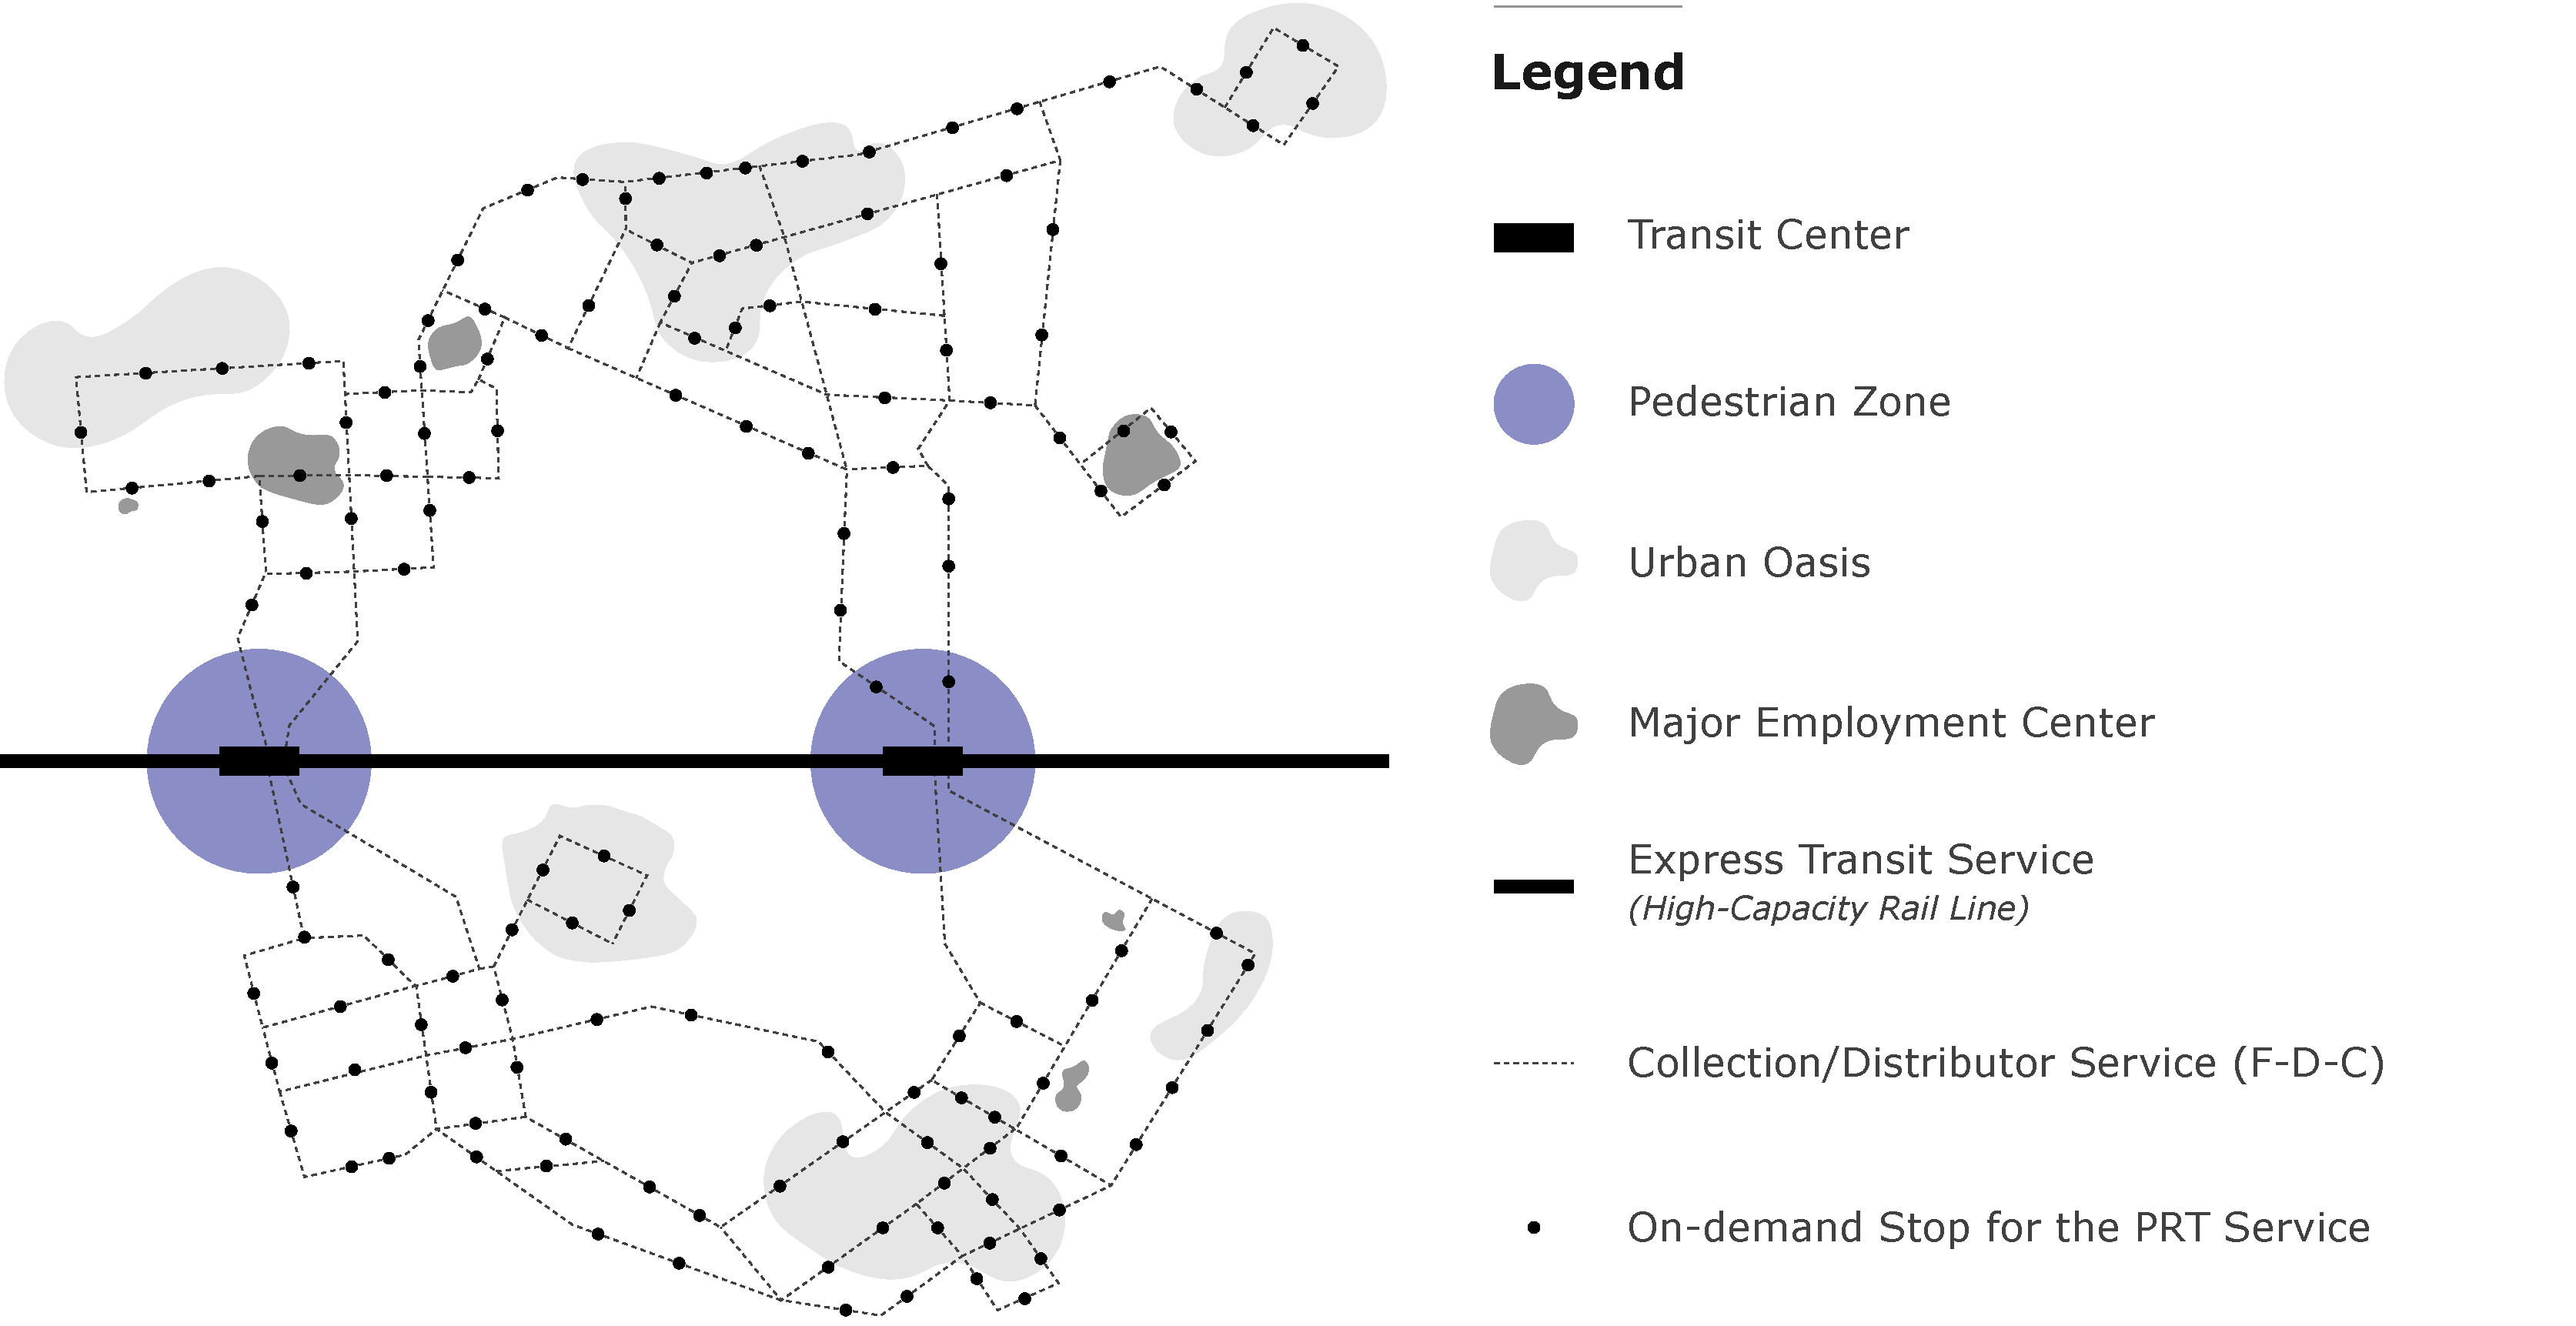
\includegraphics[width=1\columnwidth]{src/Figures/Chap-1/EN_Schema_Schneider.pdf}}
        \vspace{5pt}
        \begin{flushright}\scriptsize{
        Source: \textcolor{blue}{\textcite[142]{schneider_prt_1992}}\index{Schneider, Jerry~B.|pagebf} (see also \textcolor{blue}{\textcite{schneider_illustrating_2012}}\index{Schneider, Jerry~B.|pagebf})
        \\
        Graphic adaptation: \textcolor{blue}{Dylan Moinse (2024)}
        }\end{flushright}
    \end{carte}

% E-TOD Limits and Transition
Nevertheless, this version of \acrshort{TOD}, while maintaining the foundational principles of the model, faces technical, material, and time-related obstacles. The \acrshort{PRT} represents an infrastructural solution that is particularly costly from a budgetary perspective and demanding in terms of implementation timelines. Besides the technological challenges it involves, \acrshort{PRT} struggles to deliver significant gains in terms of congestion reduction, thus undermining its promise of more sustainable mobility and urbanism. For similar reasons, shared autonomous vehicles, which are increasingly featured in projections of a reworked rail-based urbanism, encounter comparable issues, driven by the illusion of a leap in public transport ridership\footnote{~
    In his doctoral thesis, \textcolor{blue}{Félix} \textcolor{blue}{\textcite[333]{carreyre_are_2023}}\index{Carreyre, Félix|pagebf}\index{Coulombel, Nicolas|pagebf}\index{Bouillaut, Laurent|pagebf} focused on evaluating the performance of services based on automated vehicles using a cost-benefit analysis framework combined with multi-agent modeling with \textsl{MATSim}. His work, conducted in the contexts of Berlin and Paris, demonstrated that the introduction of autonomous taxis could worsen congestion in Berlin. Moreover, in the case of Saclay, an intermodal scenario combining these services with the rail system would only increase the average occupancy rate of vehicles, although this would come at the expense of bus usage.
}. In this context, bicycles appear as a more agile and concrete solution that has proven itself in various \textsl{Hybrid Transit Metropolises} around the world. This individual mode of transport, inherently \Commas{door-to-door} and demand-driven, proves to be not only complementary to \acrshort{TOD}, but also much less costly in both economic and temporal terms. Moreover, its integration into urban mobility policies relies on relatively light and adaptable infrastructures. In this perspective, a survey conducted by \textcolor{blue}{\textcite[119]{goletz_intermodality_2020}}\index{Goletz, Mirko|pagebf}\index{Haustein, Sonja|pagebf}\index{Wolking, Christina|pagebf}\index{L'Hostis, Alain|pagebf} in Berlin, Copenhagen, Hamburg, and Paris supports the intermodal potential of cycling within a rail-oriented urbanism. The results show that specialists and researchers interviewed attribute the most promising role to cycling for effectively connecting rail infrastructures, with the notable exception of Paris, where intermodality with urban public transport networks is more widely favored. Building on the thesis of \textsl{Hybrid Transit Metropolises}, profoundly renewed by innovations in mobility, this doctoral research thus aims to examine the role of cycling as a relevant mobility solution to address the challenges of the \Commas{first and last miles.} In doing so, it also seeks to explore the progressive return of cycling to prominence through its modal diversification, around its variations, as well as the reintroduction of electric scooters, updated by advances in electromobility.%%Translated%%

% ___________________________________________
% 1.2.
\newpage
\needspace{1\baselineskip} % Reserve space
\sectionheader{The Resurgence of Light Individual Mobility}
\section{The (Re)birth of a Family of Lightweight Vehicles Designated as \Commas{Light Individual Mobility}, with Shifting Boundaries
    \label{chap1:mobilite-individuelle-legere}
    }

    % Introduction
This section offers a cross-sectional view of the evolving trajectories of the \Commas{small queen} and the \Commas{new queen}, adopting a historical perspective. It highlights the key moments in the technical and social evolution of these two modes of transport. We will particularly focus on understanding how and why these bicycles, long considered leisure objects, have gradually gained legitimacy—still under construction—in daily mobility practices. This rehabilitation takes place in a context of evolving uses and values, as well as in the context of technical and social innovations related to forms of \Commas{retro-innovation} \textcolor{blue}{\autocite{barthelot_retro-innovation_2018}}\index{Barthelot, Bertrand|pagebf}. Although these two objects share a history marked by cycles of rising popularity and withdrawal, they are experiencing a revival today, driven both by technical advancements and by transformations in urban practices. As \textcolor{blue}{Arnaud} \textcolor{blue}{\textcite[26]{passalacqua_monde_2011}}\index{Passalacqua, Arnaud|pagebf}, university lecturer and co-director of the \acrfull{EUP}, points out, urban mobility is a \Commas{\textsl{world where new solutions are often merely reprises of old forms and which, probably unintentionally, maintains a confusion between the old and the contemporary, the past and the future. By focusing on vehicles more than on systems in their entirety, this world remains confused. The vocabulary used, almost frozen since the 19\textsuperscript{th} century, contributes to reinforcing this confusion}}.%%Translated%%

% Innovation Cycles
This observation provides an opportunity to explore the reflections on \Commas{models} and \Commas{innovation cycles} \textcolor{blue}{\autocite[]{schumpeter_theorie_1911}}\index{Schumpeter, Joseph Aloïs|pagebf}, while placing them in a historical, philosophical, and ethical perspective. The Austrian and American economist \textcolor{blue}{Joseph Aloïs} \textcolor{blue}{\textcite[107]{schumpeter_capitalisme_1942}}\index{Schumpeter, Joseph Aloïs|pagebf} illustrates this dynamic through his famous concept of \Commas{creative destruction}, the engine of economic growth through innovation in products, processes, production methods, markets, or raw materials. He observes that \Commas{\textsl{the history of transportation, from the stagecoach to the airplane} [\dots] \textsl{constitutes other examples of the same industrial transformation process} [\dots] \textsl{which incessantly revolutionizes the economic structure from within, continually destroying its aged elements and continually creating new ones.}}. As the researcher in political philosophy and history of ideas \textcolor{blue}{Thierry} \textcolor{blue}{\textcite{menissier_innovations_2021}}\index{Ménissier, Thierry|pagebf} addresses in his work \textsl{Innovations: A Philosophical Inquiry}, innovation is not limited to responding to pre-existing needs; it also acts on the collective imagination and stimulates interest in the \textsl{different}, in order to support emerging projects. Thus, it is about reflecting on the ways to better articulate the transfer and territorialization of innovations, as well as their implementation. In other words, this involves questioning the conditions of their deployment across all segments of society \textcolor{blue}{\autocite[5]{baron_thierry_2022}}\index{Baron, Nacima|pagebf}. This territorialization of innovations has been studied by \textcolor{blue}{\textcite[13]{castex_prise_2017}}\index{Castex, Élodie|pagebf}\index{Frère, Séverine|pagebf}\index{Groux, Annette|pagebf}, particularly through transport planning. Their study supports the gap between the slow shift of public actors in considering new mobility modes—such as \acrfull{STP}—in urban and mobility management tools, and the rapid evolution of needs and innovations driven by private actors.%%Translated%%

% Outline Announcement
In this section, we will examine the evolution of the bicycle and the scooter, considered both as technical and social objects, as well as their place and usage in various territories, depending on urbanization contexts (\hyperref[chap1:proximite-velo-trottinette]{section on the \Commas{golden age} of these vehicles, followed by their decline and \Commas{comeback}}, page~\pageref{chap1:proximite-velo-trottinette}). From this brief historical digression, we will review the main contemporary innovations that have marked these vehicles, notably their electrification and their sharing model in public spaces (\hyperref[chap1:velo-micromobilite-innovations]{section on the diversification and \Commas{modal hybridization} of bicycles}, page~\pageref{chap1:velo-micromobilite-innovations}). Finally, we will contextualize the revival of the bicycle and the scooter, in their various forms, in a \Commas{liquid} society, driven by generations increasingly inclined towards \gls{multimodality}. This framework will also allow us to propose our own definition of this family of vehicles, by delineating more precise conceptual boundaries. This definition aims to integrate the vehicles we identify as having the greatest strategic potential to strengthen and redeploy the principles of \acrshort{TOD} (\hyperref[chap1:caracterisation-mobilite-individuelle-legere]{section on the characterization of a class of vehicles called \Commas{light individual mobility}}, page~\pageref{chap1:caracterisation-mobilite-individuelle-legere}).%%Translated%%

% 1.2.1.
\needspace{1\baselineskip} % Reserve space
\subsection{Evolution of the Design and the Role of the Bicycle among Utility Travel Modes
    \label{chap1:proximite-velo-trottinette}
    }

    % Introduction
Before becoming fully established as urban transport modes in their own right, bicycles and scooters went through more than a century of evolution, marked by both technical innovations and transformations in mobility practices and imaginaries in Europe. Over time, these cycles have experienced paradigms influenced by the social constructs associated with vehicles \textcolor{blue}{\autocite[13]{heran_retour_2015}}\index{Héran, Frédéric|pagebf}. Successive waves have gradually propelled them into daily mobility practices. This subsection, dedicated to a brief chronology of their evolution, aims to better situate these vehicles in their historical and urban context. To this end, we rely on the sequential reading proposed by French historian and sociologist \textcolor{blue}{Catherine} \textcolor{blue}{\textcite[]{bertho-lavenir_voyages_2011}}\index{Bertho-lavenir, Catherine|pagebf}, structured around four periods in the evolution of cycling practice: \Commas{the age of the velocipede} or the fashionable invention (from 1814 to the 1880s); \Commas{the age of the bicycle} or bourgeois leisure (from the 1880s to 1914); \Commas{the age of the bicycle} embedded in daily and tourist mobility (from 1914 to the 1970s); and \Commas{the age of the automobile} or the bicycle as a sport and leisure activity (since 1970). The intention is to provide a cross-sectional reading of the bicycle and the scooter, which share common origins and similar trajectories. These two families of transport modes have experienced a comparable fate when the modern city, with its spatial-temporal spread and increasing travel speeds, was built around urban forms that became inaccessible and ill-suited for these vehicles.%%Translated%%

% 1.2.1.1.
\needspace{1\baselineskip} % Reserve space
\subsubsection*{\Commas{The Golden Age} of the \Commas{Small Queen}
    \label{chap1:proximite-velo-trottinette-chronologie}
    }

    % Bicycle Bourgeois Leisure
\textsl{The Ages of the Velocipede and the Bicycle}. The origins of the bicycle and scooter can be traced back to the invention of the \Commas{running machine} (\textsl{Laufmaschine}), designed in 1817 by the Baden baron \textcolor{blue}{Karl Drais von Sauerbronn}\footnote{~
    He drew upon the idea of the \Commas{céléripède}, literally \Commas{the fast-walker}, from French engineer \textcolor{blue}{Joseph Nicéphore Niepce} \textcolor{blue}{\autocite{puech_bicyclette_2016}}\index{Puech, Chantal|pagebf}. In reality, some inventions predating the one commonly attributed to the \Commas{father of the bicycle} reveal that the concept of this device, based on the use of the wheel, dates back centuries. Among these predecessors, \textcolor{blue}{Leonardo da Vinci} sketched, around 1490, plans for a wooden machine resembling the modern bicycle. This prototype featured a seat, two wheels, and pedals, already reflecting an idea of mechanized individual transportation \textcolor{blue}{\autocite[9]{hills_bicycle_2004}}\index{Hills, Larry|pagebf}.
}. He sought to develop a \Commas{horse-less carriage} that was both efficient and economical \textcolor{blue}{\autocite[24]{heran_retour_2015}}\index{Héran, Frédéric|pagebf}, with the origin of this idea primarily associated with a shortage of horses due to particularly cold summers. Thus, the roots of the bicycle are closely tied to those of the scooter through their common ancestor, the \Commas{velocipede}, known in France as the draisienne and in England as the \textsl{dandy-horse}\footnote{~
    In 1818, an import patent application for the \Commas{running machine} was filed in France, under the supervision of \textcolor{blue}{Louis-Joseph Dineur}. It was also during this period that the first draisiennes appeared in Paris, accompanied by a notable advertising campaign and public events, such as the first race organized at the Luxembourg Gardens \textcolor{blue}{\autocite[141]{kobayashi_histoire_1993}}\index{Kobayashi, Keizo|pagebf}. At the time, the term \Commas{velocipede} was used pejoratively, especially in the press and in comedic performances. However, this word has endured and is still used today to refer to the wooden bicycle, which has neither pedals nor a transmission chain, and is used by children to learn balance and independence \textcolor{blue}{\autocite[21]{jouenne_quest-ce_2022}}\index{Jouenne, Noël|pagebf}.
} (see \hyperref[fig-chap1:frise-chronologique-velo-trottinette]{Figure~\ref{fig-chap1:frise-chronologique-velo-trottinette}}, page~\pageref{fig-chap1:frise-chronologique-velo-trottinette}). This rudimentary vehicle, consisting of two wheels connected by a wooden frame and powered by foot force, experienced limited success among the bourgeoisie and eventually fell into relative obscurity. Its weight and the instability of its wooden wheels made it impractical. From the late 19\textsuperscript{th} century, the bicycle and scooter took distinct trajectories, marking their own identities. On one hand, the \Commas{Michaudine}, with pedals added to a draisienne as early as 1861, popularized the bicycle among the affluent classes (see \hyperref[fig-chap1:frise-chronologique-velo-trottinette]{Figure~\ref{fig-chap1:frise-chronologique-velo-trottinette}}, page~\pageref{fig-chap1:frise-chronologique-velo-trottinette}), through \textsl{leisure} and sports clubs as well as velodromes \textcolor{blue}{\autocite[15-43]{dauncey_french_2012}}\index{Dauncey, Hugh|pagebf}. This evolution led to the \Commas{véloce}, followed by the \Commas{bicycle} in 1866, the \Commas{Grand-Bi} in 1871, and finally the modern bicycle in 1891 \textcolor{blue}{\autocite[27]{heran_retour_2015}}\index{Héran, Frédéric|pagebf}. On the other hand, the history of the scooter is more fragmented: it initially emerged as a toy for children, as early as 1895. For example, the Swiss company \Marque{Wisa-Gloria AG}, founded in 1882 and specializing in toys, was one of the pioneers in the production of scooters for children \textcolor{blue}{\autocite{schweizerisches_nationalmuseum_draisine_2018}}\index{Schweizerisches Nationalmuseum@\textsl{Schweizerisches Nationalmuseum}|pagebf}. The first scooters, resembling those of today, also appeared around 1895. These toys, made of wood and without motors, were equipped with handlebars and two or three wheels (see \hyperref[fig-chap1:frise-chronologique-velo-trottinette]{Figure~\ref{fig-chap1:frise-chronologique-velo-trottinette}}, page~\pageref{fig-chap1:frise-chronologique-velo-trottinette}). They worked through human energy: one foot rested on the board while the other pushed off the ground to propel the user.%%Translated%%

% Scooter Bourgeois Leisure
In parallel, the first scooter models, intended for the children of wealthy families, inaugurated a wave of two-wheeled scooters marketed just before the Great War \textcolor{blue}{\autocite{jeux_et_compagnie_histoire_2013}}\index{Jeux et Compagnie@\textsl{Jeux et Compagnie}|pagebf}. Although the scooter initially retained a status as a toy, it gradually appealed to a broader audience, reaching children from less privileged social classes \textcolor{blue}{\autocite{historia_trottinette_2013}}\index{Historia@\textsl{Historia}|pagebf}. During the interwar period, metallic models with pneumatic tires appeared and were patented, incorporating technical innovations inspired by those of the bicycle \textcolor{blue}{\autocite{arte_histoire_2014}}\index{Arte@\textsl{Arte}|pagebf}. In terms of their relationship with the social world, both the bicycle and the scooter were initially associated with bourgeois practices\footnote{~
    Although the initial development of the bicycle was driven by the upper classes, these groups experienced a sense of injustice linked to a lack of legitimacy on the road. In his doctoral thesis on the history of road usage, \textcolor{blue}{Jean} \textcolor{blue}{\textcite[126-132, 327]{orselli_usages_2008}}\index{Orselli, Jean|pagebf} highlights the challenges faced by cyclists at the end of the 19\textsuperscript{th} century. These difficulties were manifested through regulations marked by a true \Commas{velophobic rage}, as well as popular violence, particularly in rural areas, between 1874 and 1896. These tensions preceded the establishment of national regulations on velocipedes, whose application by municipalities, however, remained largely ignored. This conflict must be understood in the context of a road historically dominated by horse-drawn carriages, which held an ancestral position and enjoyed tacit respect, both from the population and the police. This situation reflects the difficult social acceptance of the bicycle in a society where the horse-drawn carriage still embodied, at the time, a prestigious means of transportation, used by the French aristocracy for centuries \textcolor{blue}{\autocite[139]{orselli_usages_2008}}\index{Orselli, Jean|pagebf}.
}. High prices and social codes reserved them for an elite seeking new leisure and exclusive sports \textcolor{blue}{\autocite[90]{bravard_cercle_2011}}\index{Bravard, Alice|pagebf}. However, with the modernization of manufacturing processes and the democratization of these objects\footnote{~
    The Japanese historian \textcolor{blue}{Keizo} \textcolor{blue}{\textcite[149]{kobayashi_histoire_1993}}\index{Kobayashi, Keizo|pagebf}, in his work titled \textsl{History of the Velocipede from Drais to Michaux 1817-1870: Myths and Realities}, sheds light on the origin of the bicycle by stating that \Commas{\textsl{among the main flaws of the velocipede, it was criticized for the fatigue it caused, its lack of balance while in motion or at rest, and the discomfort from the vibrations.}} In response to these limitations, various technical solutions were considered to alleviate the physical effort and improve the user experience. Improvement inventions multiplied, ranging from enhancing energy transmission by improving traction with the front wheel and propulsion with the rear wheel, to the link chain with gears in 1829, the addition of solid rubber tires in 1869 \textcolor{blue}{\autocites{inpi_draisienne_2020}[38]{jouenne_quest-ce_2022}}\index{Jouenne, Noël|pagebf}\index{INPI@\textsl{INPI}|pagebf}, and the invention of the pneumatic tire with an air chamber in 1888 \textcolor{blue}{\autocite[14]{papon_retour_2012}}\index{Papon, Francis|pagebf}. However, the advances in the velocipede were not solely technical. Its social and cultural development was largely supported by popular events, such as public demonstrations and cycling races, which helped increase its visibility and contributed to its gradual adoption by a wider public.
}, the bicycle and scooter eventually expanded to lower social classes, gradually losing their status as social distinction objects, characteristic of a \Commas{bourgeois culture}.%%Translated%%

% Bicycle Popularization
\textsl{The Age of the Bicycle}. During the Belle Époque and even more so during the Roaring Twenties, cycle tourism became a popular activity in Europe, particularly through the organization of bicycle tours taking the form of weekend itinerant camps \textcolor{blue}{\autocite[26]{eskenazi_voir_2022}}\index{Eskenazi, Manon|pagebf}, as well as with the arrival of the first paid vacations in 1936 \textcolor{blue}{\autocite[108]{dauncey_french_2012}}\index{Dauncey, Hugh|pagebf}. Cyclists could then park their bicycles at inns overnight, a practice that spread particularly in Germany \textcolor{blue}{\autocite[327]{herlihy_bicycle_2004}}\index{Herlihy, David|pagebf}. Between 1918 and the 1950s, the modern bicycle became popular among the working classes, inaugurating a major social innovation: daily bicycle commuting, now seen as a realistic alternative \textcolor{blue}{\autocite[31]{jouenne_quest-ce_2022}}\index{Jouenne, Noël|pagebf}. These commuting trips, especially those of workers, helped reduce travel times while offering more free time. This popularity increased during the Great Depression of the 1930s, due to rising fuel prices and the inability of many households to afford automobile ownership. In the United States, where the bicycle had previously been considered a vehicle for children, it experienced significant growth \textcolor{blue}{\autocite[327]{herlihy_bicycle_2004}}\index{Herlihy, David|pagebf}. Thanks to its ease of use and speed, demand and production of bicycles surged. Between 1894 and 1934, the number of bicycles in circulation increased 32-fold \textcolor{blue}{\autocite[32]{papon_retour_2012}}\index{Papon, Francis|pagebf}. In many European countries, the bicycle became the dominant mode of transport. In Copenhagen, 33\% of the population used bicycles in 1930, while in the Netherlands, 3 million bicycles were in circulation, equivalent to the country's population. In France and the UK, around 7 million bicycles were sold, compared to 15 million in Germany. Japan had 6 million users, while in the United States and China, bicycle use developed gradually \textcolor{blue}{\autocite[329]{herlihy_bicycle_2004}}\index{Herlihy, David|pagebf}. In this context, industrial clusters emerged. Saint-Étienne, for example, became the \Commas{Bicycle Capital}, with over a hundred factories producing about 80\% of the bicycles manufactured in France \textcolor{blue}{\autocite[328]{herlihy_bicycle_2004}}\index{Herlihy, David|pagebf}. In the immediate post-war period, the bicycle continued to be widely used in European cities. Sweden, in particular, emerged as the world’s leading cycling nation.%%Translated%%

% Popularization of the Folding Bicycle
It is impossible to discuss the bicycle and the technical innovations that marked it without mentioning the simultaneous development of the folding bicycle. The first patent for a folding bicycle was granted to the American engineer \textcolor{blue}{Emmit G. Latta} in 1887, although traces of a detachable Grand-Bi date back to 1878 \textcolor{blue}{\autocite{the_folding_cyclist_history_2010}}\index{The Folding Cyclist@\textsl{The Folding Cyclist}|pagebf}. This concept addressed the need to facilitate bicycle storage by reducing its bulk, although it was initially intended primarily for military use\footnote{~
    The French industrialist \textcolor{blue}{Charles Morel} developed a prototype of a folding bicycle in 1892, which, in collaboration with Lieutenant \textcolor{blue}{Henri Gérard}, was intended for military use \textcolor{blue}{\autocite{the_folding_cyclist_history_2010}}. Presented at the Salon du Cycle in Paris in 1894, the \Marque{Capitaine Gérard} model was adopted by the French army and became part of the infantry’s equipment (see \hyperref[fig-chap1:frise-chronologique-velo-trottinette]{Figure~\ref{fig-chap1:frise-chronologique-velo-trottinette}}, page~\pageref{fig-chap1:frise-chronologique-velo-trottinette}). This first generation of folding bicycles, presented as an asset compared to the horse, was called the \Commas{Bicyclette pliante}. Its ability to fold up and be carried on the back using straps made it a practical solution that did not require infrastructure such as stables or garages.
}. In France, the Peugeot brand marketed a lightweight adult folding bicycle, but was unable to make it truly popular with the general public \textcolor{blue}{\autocite{transportation_alternatives_folding_2013}}\index{Transportation Alternatives@\textsl{Transportation Alternatives}|pagebf}. The real reduction in the size of the folding bicycle's wheels, inspired notably by the \Marque{Katakura} bicycles in Japan, only occurred from the 1920s, marking the start of its wider distribution. The bicycle continued to benefit from continuous improvements, with a patent filed in 1944 for a folding and detachable bicycle equipped with small wheels. This model, described by the press of the time under the name \Marque{Petit-Bi}, was presented as a major advancement \textcolor{blue}{\autocite[44]{jouenne_quest-ce_2022}}\index{Jouenne, Noël|pagebf}. The press noted that the \Marque{Petit-Bi} \Commas{\textsl{would mark a milestone in the history of cycling due to the clear advantages it presented}} \textcolor{blue}{\autocite{the_folding_cyclist_history_2010}}\index{The Folding Cyclist@\textsl{The Folding Cyclist}|pagebf}.%%Translated%%

% Figure Bicycle-Scooter Timeline
\begin{figure}[h!]\vspace*{4pt}
        \caption{Joint evolution of the bicycle and scooter from a historical perspective.}
        \label{fig-chap1:frise-chronologique-velo-trottinette}
        \centerline{\includegraphics[width=1\columnwidth]{src/Figures/Chap-1/EN_Chronologie_velo_trottinette.pdf}}
        \vspace{5pt}
        \begin{flushright}\scriptsize{
        Photography (A): \textcolor{blue}{\textcite{smithsonian_draisine_2006}}\index{Smithsonian@\textsl{Smithsonian}|pagebf}
        \\
        Photography (B): \textcolor{blue}{\textcite{conservatoire_national_des_arts_et_metiers_velocipemichaux_2013}}\index{Conservatoire national des arts et métiers@\textsl{Conservatoire national des arts et métiers}|pagebf}
        \\
        Photography (C): \textcolor{blue}{\textcite{chateau_de_compiegne_grand-bi_nodate}}\index{Château de Compiègne@\textsl{Château de Compiègne}|pagebf}
        \\
        Photography (D): \textcolor{blue}{Kristy von} \textcolor{blue}{\textcite{moos_parcours_2019}}\index{Moos, Kristy von|pagebf}
        \\
        Photography (E): \textcolor{blue}{\textcite{alienor_bicyclette_2015}}\index{Alienor@\textsl{Alienor}|pagebf}
        \\
        Photography (F): \textcolor{blue}{Dylan Moinse (2023)}
        \\
        Photography (G): \textcolor{blue}{\textcite{musee_national_suisse_draisienne_2018}}\index{Musée national suisse@\textsl{Musée national suisse}|pagebf}
        \\
        Photography (H): \textcolor{blue}{\textcite{zerorider_lautoped_2023}}\index{Zerorider@\textsl{Zerorider}|pagebf}
        \\
        Author: \textcolor{blue}{Dylan Moinse (2025)}
      }\end{flushright}
    \end{figure}

    % E-Bike
What about the \acrfull{e-Bike}? Its origins date back only fifteen years after the invention of the bicycle chain. The first prototype is attributed to \textcolor{blue}{Odgen Bolton Jr.}, who, in the United States, patented a draisienne in 1895 equipped with a six-pole direct current motor integrated into the rear wheel and powered by a ten-volt battery placed under the horizontal frame tube \textcolor{blue}{\autocites[3]{hung_review_2020}{adelski_qui_2023}}\index{Hung, Nguyen Ba|pagebf}\index{Lim, Ocktaeck|pagebf}\index{Adelski, Adeline|pagebf}. The second generation of \acrshort{e-Bike} emerged in 1897 with the invention of \textcolor{blue}{Hosea W. Libbey}, who designed the \Marque{Lampociclo}, a bicycle equipped with a dual electric motor housed in the pedal axle. The operation of this innovation was based on a generator powered by the pedals via a pulley and flexible belt. The energy produced then powered a small electric motor \textcolor{blue}{\autocite[3]{hung_review_2020}}\index{Hung, Nguyen Ba|pagebf}\index{Lim, Ocktaeck|pagebf}. However, several attempts at improvement failed, notably one by \Marque{Compagnie Parisienne}, which developed a \acrshort{e-Bike} model around the same time but encountered issues with an excessive weight \textcolor{blue}{\autocite[78]{hadland_bicycle_2016}}\index{Hadland, Tony|pagebf}\index{Lessing, Hans-Erhard|pagebf}. At the end of World War I, the German company \Marque{Heinzmann} launched the first mass production of electric motors for bicycles, equipping, among others, the country’s postal workers. Between 1935 and 1937, the first series model, the \Marque{EMI/Philips}, was marketed, but its performance remained limited compared to the competition from automobiles \textcolor{blue}{\autocite[143]{smethurst_bicycle_2015}}\index{Smethurst, Paul|pagebf}.%%Translated%%

% Popularization of the Motorized Scooter
In the realm of fascination with innovative objects, the case of the birth of the motorized scooter in 1915 deserves particular attention. It was the New York-based company \Marque{Autoped Company} that launched the first model of scooter equipped with a gasoline engine (see \hyperref[fig-chap1:frise-chronologique-velo-trottinette]{Figure~\ref{fig-chap1:frise-chronologique-velo-trottinette}}, page~\pageref{fig-chap1:frise-chronologique-velo-trottinette}). This vehicle met with immediate success, sparking interest among adults curious to discover this vehicle, initially produced in the United States and later in Europe by the German manufacturer \Marque{Krupp} starting in 1919. Advertisements promoting its use in various professions quickly appeared\footnote{~
    Photographs show \textsl{US Postal Office} postal workers and US police officers integrating this technical object into their daily duties after the Great War \textcolor{blue}{\autocite{ma_trott_origines_2019}}.
}. The \textsl{Online Bike Museum} refers to the \Marque{Autoped} model as the \Commas{true ancestor of the electric scooter}, as it foreshadows the modern form of this vehicle. However, at its launch, the cycling press rejected this technical innovation, labeling the \Marque{Autoped} as \Commas{monster vehicles} doomed to failure. Despite these criticisms, motorized scooters, through a fashion effect, managed to gain popularity until the end of the Roaring Twenties \textcolor{blue}{\autocite{smithsonian_magazine_motorized_2019}}\index{Smithsonian Magazine@\textsl{Smithsonian Magazine}|pagebf}. Advertisements of the time highlighted the numerous potential uses of this mode of transport. They presented the \Marque{Autoped} as an ideal solution for short trips, both for men and women going to work and for children wishing to quickly get to school. The slogan \Commas{\textsl{The Autoped is an ideal short-distance conveyance for business or professional men or women to and from their places of business; for women to go shopping} [\dots] \textsl{for the older children to go about quickly for outing or school} [\dots] \textsl{and for anybody else who wants to save money, time and energy in going about.}}\footnote{~
    \Commas{\textsl{The Autoped is an ideal short distance conveyance for business or professional men or women to and from their places of business; for women to go shopping} [\dots] \textsl{for the older children to go about quickly for outing or school} [\dots] \textsl{and for anybody else who wants to save money, time and energy in going about.}} \textcolor{blue}{\autocite{smithsonian_magazine_motorized_2019}}.
} reflects the ambition to promote the motorized scooter as a practical and accessible vehicle \textcolor{blue}{\autocite{smithsonian_magazine_motorized_2019}}\index{Smithsonian Magazine@\textsl{Smithsonian Magazine}|pagebf}. The \textsl{marketing} strategy of \Marque{Autoped} sought to attract a female audience\footnote{~
    The painting by artist \textcolor{blue}{Everett Shinn} depicting a woman riding an \Marque{Autoped} scooter on the cover of \textsl{Puck magazine} in 1916, or photographs of celebrities such as actress \textcolor{blue}{Lilian Lorraine} owning one of these vehicles, testify to the popular interest sparked by the thermal propulsion scooter \textcolor{blue}{\autocite{hemmings_look_2011}}. The communication surrounding this product reveals the intention to associate it with a distinct social class. The user is typically depicted as a white, affluent woman dressed in the style of the time.
} by integrating the vehicle into catalogs aimed at women and entering the world of fashion. Some of the brand's advertisements also spread the image of women's freedom of movement, gained thanks to the device \textcolor{blue}{\autocite{smithsonian_magazine_motorized_2019}}\index{Smithsonian Magazine@\textsl{Smithsonian Magazine}|pagebf}. The commercialization of this product, originating from the United States, spread to Europe, in contrast to the historical trajectory taken by the diffusion of the bicycle, as we have seen. However, its history ended abruptly at the end of the 1920s. The arrival of new battery-powered versions did not suffice to ensure the profitability of the device, due to the growing competition from bicycles and mopeds, which offered superior comfort and were more suited to the needs of the time.%%Translated%%

% 1.2.1.2.
\needspace{1\baselineskip} % Reserve space
\subsubsection*{From the Decline of Utility Bicycles to their Resurgence in Daily Commuting Practices
    \label{chap1:proximite-velo-trottinette-declin-renaissance}
    }

    % Introduction
With the improvement of living standards, easier access to automobiles starting in the 1950s, and a depreciated image of the bicycle, developed countries experienced a \Commas{general collapse} of cycling practices during the second half of the 20\textsuperscript{th} century \textcolor{blue}{\autocites[59-84]{heran_retour_2015}[9-10]{heran_retour_2024}}\index{Héran, Frédéric|pagebf}. After World War II, the bicycle was seen as a symbol of poverty, associated with the mobility of workers, but also as a reminder of deprivation and conflict, leaving behind a dated and unflattering image in the collective imagination. This \gls{perception} sharply contrasts with the speed and modernity embodied by the automobile, which was seen as a vehicle for social ascension \textcolor{blue}{\autocite[59]{bertho-lavenir_scarcity_2015}}\index{Bertho-lavenir, Catherine|pagebf}. During the Trente Glorieuses, the car emerged as a symbol of modernity and innovation, conveying ideals of progress \textcolor{blue}{\autocite[35]{flonneau_georges_1999}}\index{Flonneau, Mathieu|pagebf}. Urban planning policies supported this growth by favoring the construction of road infrastructure adapted to the projected, even exaggerated, increase in automobile traffic \textcolor{blue}{\autocite[58]{wiel_transition_1999}}\index{Wiel, Marc|pagebf}. The widespread adoption of the automobile profoundly transformed cities and their spatial organization. The areas people frequented expanded, increasing the spatial-temporal distances needed for daily activities, thanks to \Commas{facilitated mobility} allowing motorized populations to settle in the periphery, particularly in suburban housing developments \textcolor{blue}{\autocite[58]{wiel_transition_1999}}\index{Wiel, Marc|pagebf}. This phenomenon of urban sprawl is inseparable from the growth of automobile use \textcolor{blue}{\autocites[8]{newman_land_1996}[3]{aragau_periurbain_2018}}\index{Aragau, Claire|pagebf}, which has led to a \Commas{land abundance} \textcolor{blue}{\autocite[20]{wiel_transition_1999}}\index{Wiel, Marc|pagebf}. This context gave rise to the formation of \Commas{edge cities}, secondary \Commas{suburban} hubs, connected to highway interchanges, which gather economic and commercial activities and compete with the central urban core \textcolor{blue}{\autocite[]{garreau_edge_1991}}\index{Garreau, Joel|pagebf}.%%Translated%%

% Decline of the Bicycle
Although the periods described do not reflect perfectly linear developments and involve underlying complex mechanisms, a nuanced reading of the opposition between functional cities and modern cities cannot overlook the gradual decline of the utility bicycle from the post-war economic boom. In France, facing a car fleet that doubled during the 1960s and reached a household motorization rate of 60\% \textcolor{blue}{\autocite[43]{flonneau_georges_1999}}\index{Flonneau, Mathieu|pagebf}, the use of bicycles as a utility transport mode significantly dropped in the 1970s, reaching a historically low level in most European cities \textcolor{blue}{\autocite[41]{eskenazi_voir_2022}}\index{Eskenazi, Manon|pagebf}. In her doctoral research dedicated to the intermodality between bicycles and public transport, \textcolor{blue}{Annie-Claude} \textcolor{blue}{\textcite[53]{sebban_complementarite_2003}}\index{Sebban, Annie-Claude|pagebf}\index{Motte, Alain|pagebf} challenges the idea that the 1980s and 1990s marked a widespread abandonment of cycling in France. In reality, this decline only concerns the utility use of bicycles, which was largely supplanted by cars in cities. This phenomenon is also explained by the statistical methods of public surveys, which did not systematically include bicycles as a full-fledged mode of transport. At the same time, new cycling dynamics emerged, particularly with the rise of \acrfull{VTT}, which became a major driver of the bicycle's resurgence in France. By 1990, \acrshort{VTT} represented 35\% of bicycles owned and 71\% of sales \textcolor{blue}{\autocite[195]{dauncey_french_2012}}\index{Dauncey, Hugh|pagebf}. Meanwhile, cycle tourism and sport cycling remained stable, showing no real decline \textcolor{blue}{\autocite[53]{sebban_complementarite_2003}}\index{Sebban, Annie-Claude|pagebf}\index{Motte, Alain|pagebf}. In France, the bicycle thus became primarily associated with leisure. Competitive cycling, notably, reached its peak in the 1980s, driven by the popularity of the \textsl{Tour de France} and its growing media presence \textcolor{blue}{\autocite[196]{dauncey_french_2012}}\index{Dauncey, Hugh|pagebf}.%%Translated%%

% Decline of the Scooter
Regarding the scooter, whether human-powered or motorized, some American companies, in the aftermath of World War II, attempted to revive the use of the motorized scooter. However, with the rise of the automobile, this vehicle was quickly accused of promoting dangerous behaviors on the road \textcolor{blue}{\autocite{smithsonian_magazine_motorized_2019}}\index{Smithsonian Magazine@\textsl{Smithsonian Magazine}|pagebf}. While the development of gasoline or battery-powered scooters remained limited to anecdotal episodes—such as the use of \Marque{Autoped} scooters by American and British paratroopers to cross battlefields during the war \textcolor{blue}{\autocite{historia_trottinette_2013}}\index{Historia@\textsl{Historia}|pagebf}, or the use of muscle-powered scooters by employees at Amsterdam-Schiphol Airport \textcolor{blue}{\autocite{historia_trottinette_2013}}\index{Historia@\textsl{Historia}|pagebf}—this motorized model failed to establish itself sustainably. In the 1950s, as the motorized scooter fell into obsolescence, efforts were made to revive the non-motorized scooter. Manufacturers tried to position it as a credible means of transport, no longer just a toy for children. To this end, some innovations appeared, such as adding a pedal at the front of the platform to activate the rear wheel and reduce physical effort \textcolor{blue}{\autocite{arte_histoire_2014}}\index{Arte@\textsl{Arte}|pagebf}. Despite these advances, the vehicle struggled to appeal to a wide audience and remained mostly perceived as a playful object or one intended for children \textcolor{blue}{\autocite{jeux_et_compagnie_histoire_2013}}\index{Jeux et Compagnie@\textsl{Jeux et Compagnie}|pagebf}. The low demand, which was part of the advent of a \Commas{car-only} system, prevented these models from finding their place in urban mobility and territories \textcolor{blue}{\autocite{historia_trottinette_2013}}\index{Historia@\textsl{Historia}|pagebf}. The imperative to adapt territories to the widespread use of the automobile relegated the scooter to an anecdotal use. Its use in cities became unsafe, both on roads and pedestrian areas, limiting its spread and reducing available information about it \textcolor{blue}{\autocite{e-trottr_levolution_2019}}\index{E-trottr@\textsl{E-trottr}|pagebf}. Despite these setbacks, vehicles in the cycling family experienced a recent resurgence as they were reintegrated into urban mobility practices.%%Translated%%

% Figure Evolution of Modal Share of Bicycles
\begin{figure}[h!]\vspace*{4pt}
    \caption{Evolution of the modal share of bicycles in French metropolitan areas, from the 1970s to 2020.}
    \label{fig-chap1:evolution-part-modale-velo}
    \centerline{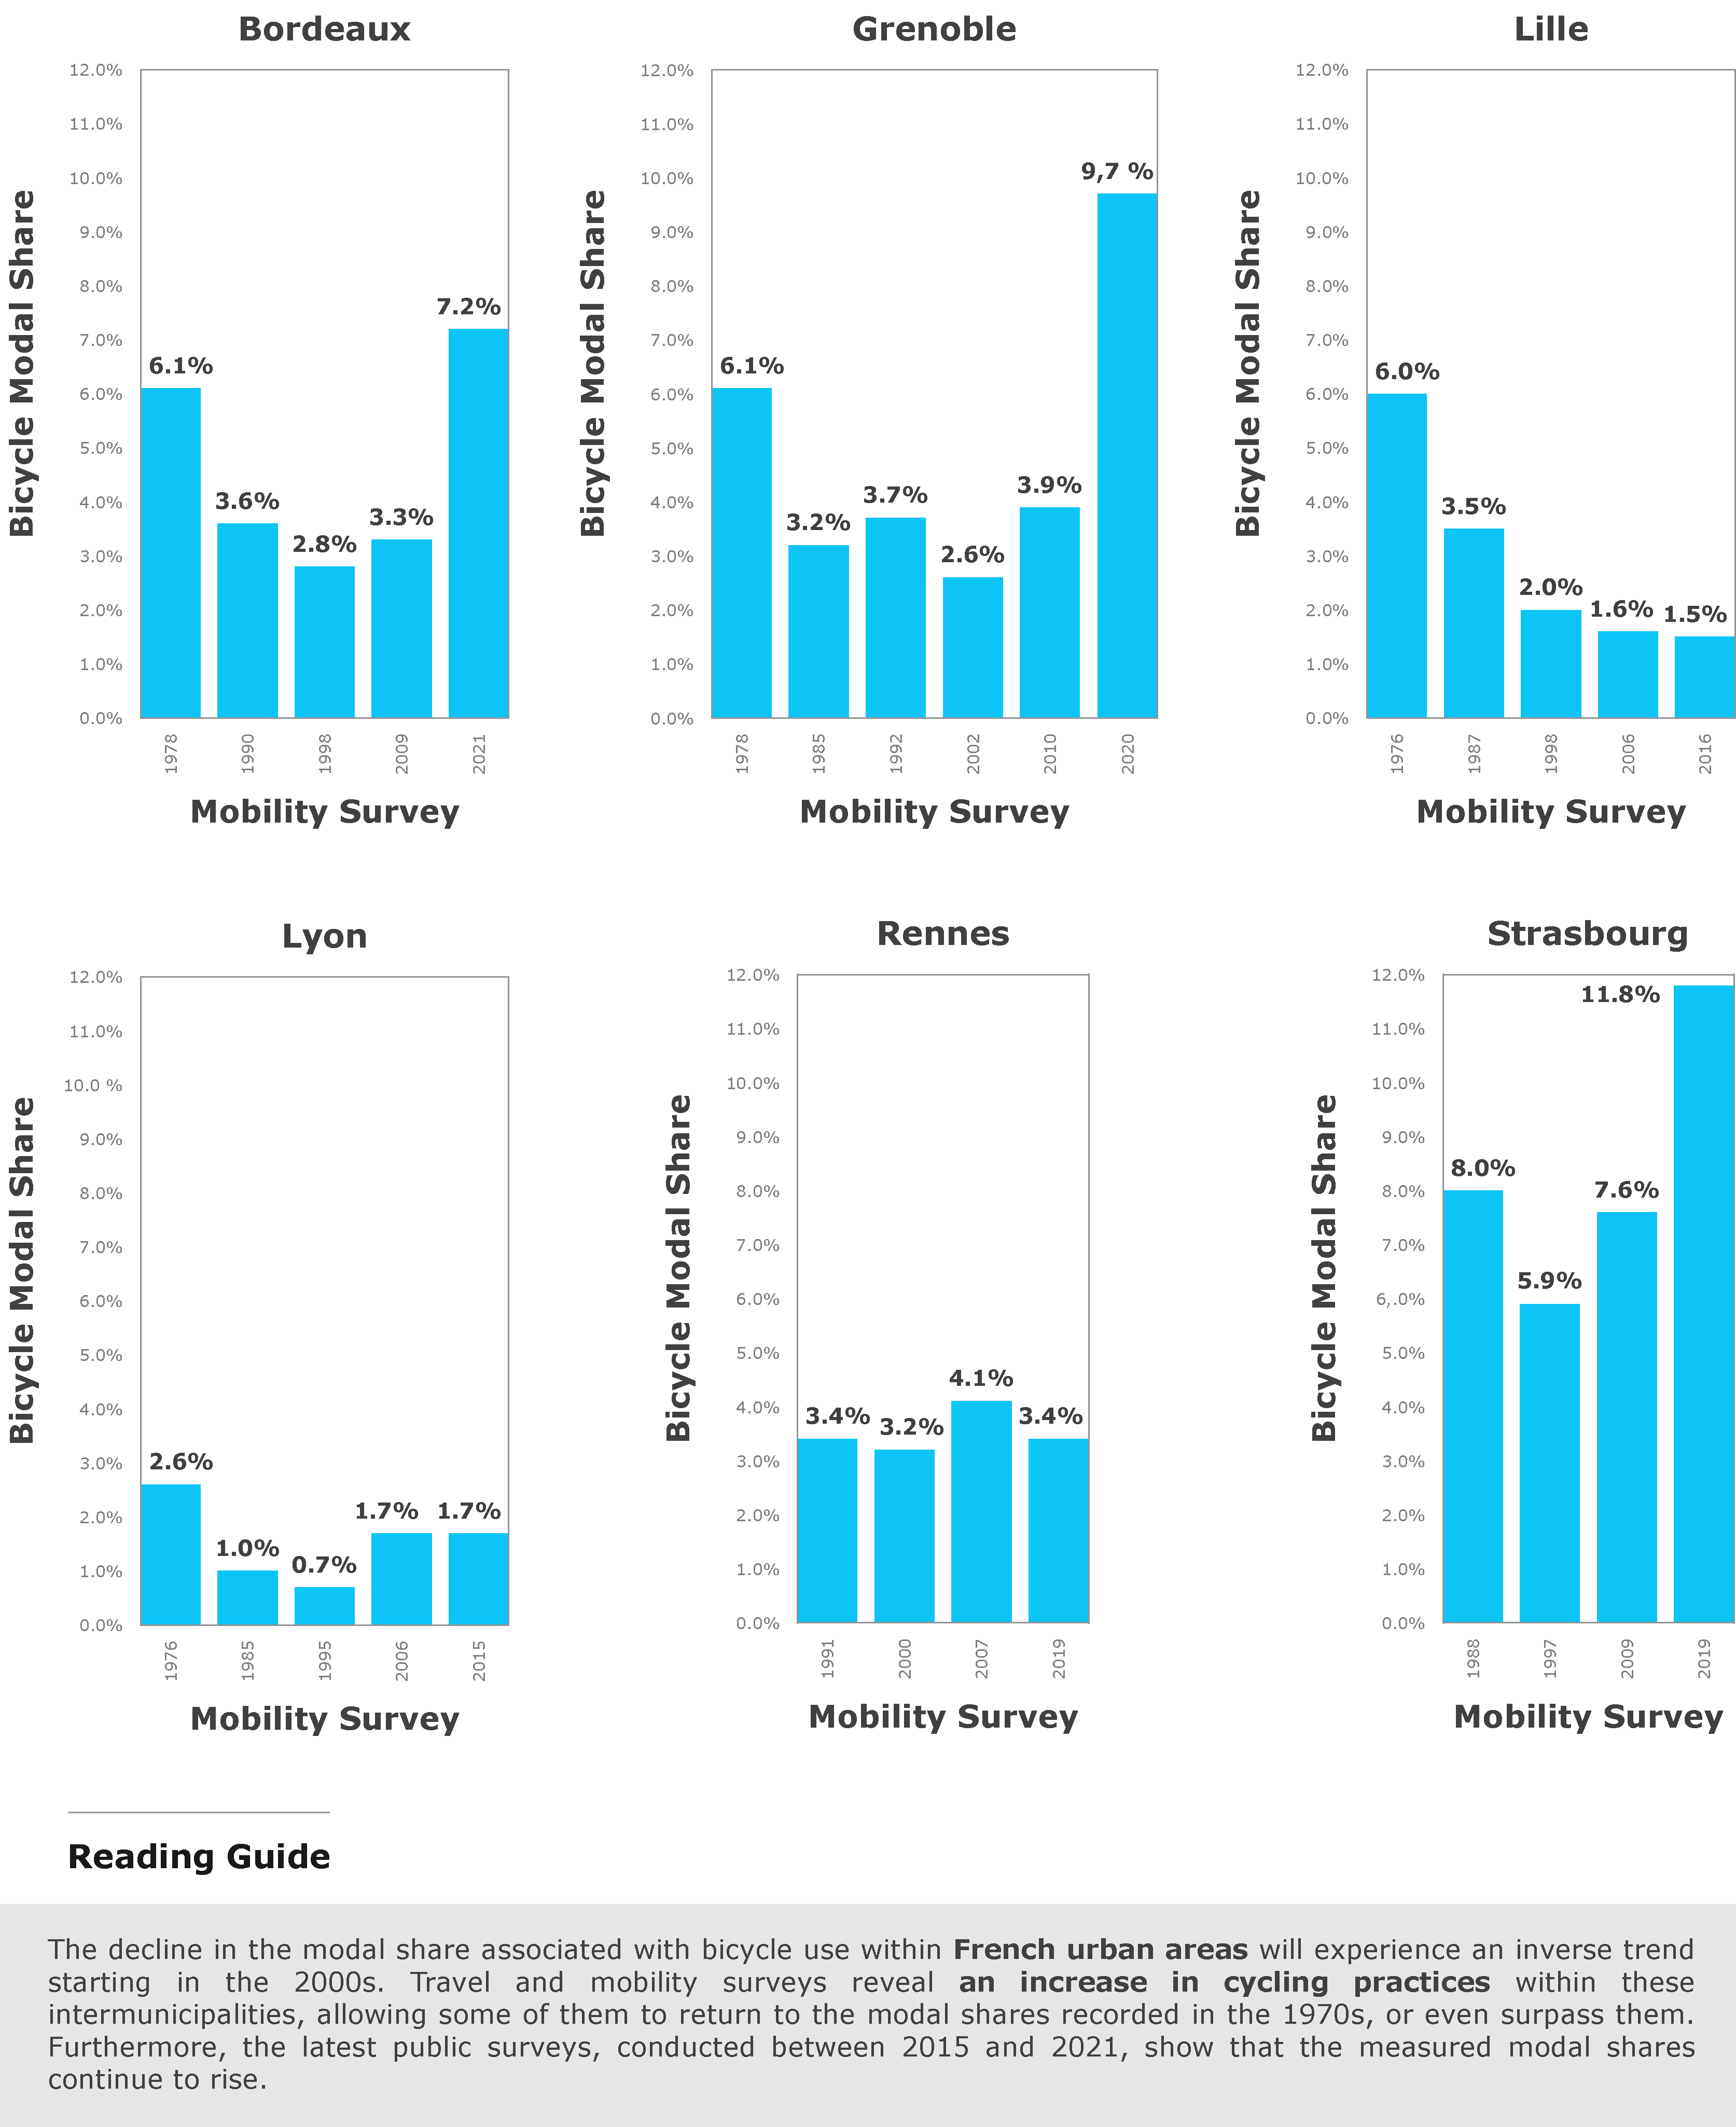
\includegraphics[width=1\columnwidth]{src/Figures/Chap-1/EN_Part_modale_velo_evolution.pdf}}
    \vspace{5pt}
    \begin{flushleft}\scriptsize{
    Note: the territories refer to their intermunicipal scale, while the mobility surveys relate to the \acrfull{EMD} corpus based on the \textsl{Certu} standard or certified by \textsl{Cerema}.
    }\end{flushleft}
    \begin{flushright}\scriptsize{
    Datasets: analysis from \textcolor{blue}{\textcite[48]{certu_usagers_2013}}\index{Certu@\textsl{Certu}|pagebf}\index{Cerema@\textsl{Cerema}|pagebf}\index{Jolly, Thomas|pagebf}
    \\
    Graphic adaptation and reinterpretation: \textcolor{blue}{Dylan Moinse (2025)}
    }\end{flushright}
\end{figure}

% Bicycle Resurgence in France
The \Commas{resurgence} of the bicycle in French territories \textcolor{blue}{\autocites[137-168]{heran_retour_2015}[44]{eskenazi_voir_2022}}\index{Héran, Frédéric|pagebf}\index{Eskenazi, Manon|pagebf} is part of a dynamic that began over forty years ago. This revival marks a second phase of conquest for the bicycle, long disqualified in daily mobility \textcolor{blue}{\autocite[26]{papon_retour_2012}}\index{Papon, Francis|pagebf}, while the utility use of the bicycle continues to decline in French cities, with a decrease of 50\% to 75\% between 1975 and 1990 \textcolor{blue}{\autocite[48]{certu_usagers_2013}}\index{Certu@\textsl{Certu}|pagebf}\index{Cerema@\textsl{Cerema}|pagebf}\index{Jolly, Thomas|pagebf}. Already in 1976, the newspaper \textsl{Le Monde} pointed out a contradiction in \Commas{mocking} the \Commas{forgotten} cyclists, while the bicycle fleet, estimated at 17 million, rivaled the number of private cars in possession \textcolor{blue}{\autocite{ambroise-rendu_creation_1976}}\index{Ambroise-Rendu, Marc|pagebf}\index{Le Monde@\textsl{Le Monde}|pagebf}. Mobility surveys conducted from the 2000s highlight a resurgence of the bicycle in daily mobility practices (see \hyperref[fig-chap1:evolution-part-modale-velo]{Figure~\ref{fig-chap1:evolution-part-modale-velo}}, page~\pageref{fig-chap1:evolution-part-modale-velo}). The Lyon metropolitan area saw the bicycle modal share quadruple between 1995 and 2006, while that of \acrfull{MEL} compensated for its decline between 1998 and 2006 \textcolor{blue}{\autocite[243]{dauncey_french_2012}}\index{Dauncey, Hugh|pagebf}. This phenomenon can be explained by growing environmental concerns, combined with the repercussions of successive economic and energy crises \textcolor{blue}{\autocite[138]{heran_retour_2015}}\index{Héran, Frédéric|pagebf}, as well as the densification of associative networks and changes in legal and regulatory frameworks \textcolor{blue}{\autocite[55]{sebban_complementarite_2003}}\index{Sebban, Annie-Claude|pagebf}\index{Motte, Alain|pagebf}. This period also saw the emergence of new types of bicycles, such as city bikes designed for urban use, or the aluminum folding bicycle \Marque{Brompton} \textcolor{blue}{\autocite[55]{sebban_complementarite_2003}}\index{Sebban, Annie-Claude|pagebf}\index{Motte, Alain|pagebf}. But it was especially the 1995 public transport strike, widely followed, that marked a decisive moment in this shift, allowing the bicycle to reposition itself as a credible alternative. The resurgence of the bicycle was accompanied by a sociological and spatial transformation: while the 1970s bicycle was mostly used by captive populations in suburban areas, the 1990s saw the emergence of users from middle and upper classes, moving within urban areas\footnote{~
    According to \textcolor{blue}{Frédéric} \textcolor{blue}{\textcite[143]{heran_retour_2015}}\index{Héran, Frédéric|pagebf}, \Commas{\textsl{In 1982, the typical cyclist was a rather young man, without a driver's license, from a large family, working-class or agricultural, often immigrant, with modest income and little or no motorized transport, living in the suburbs or a provincial town. He rode his bike to school or work, dreaming of buying a moped and, one day, a car. According to the results of the 2007-2008 ENTD, these users are still mostly men (63\%), but now mostly public service executives and professionals, much more rarely workers or employees.}}. Moreover, urban cyclists replaced the \Commas{proletarians of traffic} \textcolor{blue}{\autocite{ambroise-rendu_creation_1976}}\index{Ambroise-Rendu, Marc|pagebf}, becoming a French specificity due to investments almost exclusively focused on city centers \textcolor{blue}{\autocite[144]{heran_retour_2015}}\index{Héran, Frédéric|pagebf}.
} \textcolor{blue}{\autocite[143]{heran_retour_2015}}\index{Héran, Frédéric|pagebf}.%%Translated%%

% Transition
Although the bicycle's modal share remains modest in France—at 3\% of trips, compared to 10\% in Germany and 27\% in the Netherlands—this period is marked by an unprecedented momentum in favor of utility cycling \textcolor{blue}{\autocite[222]{dauncey_french_2012}}\index{Dauncey, Hugh|pagebf}. Local initiatives such as Strasbourg's \textsl{Plan vélo}, which transformed a fragmented cycling network into a continuous mesh of 483 km in 2006, illustrate this dynamic. Since the 2010s, the bicycle has become deeply linked to environmental and public health issues. In the face of urban pollution and car congestion, it is seen as an environmentally low-impact solution, beneficial for public and economic health. Efforts to promote its development reflect a desire to foster true \Commas{ecomobility} \textcolor{blue}{\autocites[4]{sebban_complementarite_2003}{heran_transition_2018}}\index{Sebban, Annie-Claude|pagebf}\index{Motte, Alain|pagebf}\index{Héran, Frédéric|pagebf}, marking a return of the \Commas{forgotten modes} to daily mobility practices \textcolor{blue}{\autocite[35]{papon_retour_2012}}\index{Papon, Francis|pagebf}. It would also have been possible to discuss the shared history of other \Commas{urban gliding objects}, such as the skateboard or roller skates\footnote{~
    This perspective differs somewhat for these other vehicles, which remain primarily associated with leisure and are not intended to meet needs for directive mobility or to share road space in a structured way.
}, but the goal here is not to provide an exhaustive analysis or to retrace the entire history of cycling. The intention is rather to connect the development of bicycles to the legacies of diffuse urban planning, shaped by the automobile. The investments made to bring the bicycle to the forefront have been accompanied by local initiatives, including the establishment of cycling infrastructure and the installation of mobility services, such as \acrshort{PBS} systems \textcolor{blue}{\autocite[244]{dauncey_french_2012}}\index{Dauncey, Hugh|pagebf}, as well as the deployment of electromobility.%%Translated%%

% 1.2.2.
\needspace{1\baselineskip} % Reserve space
\subsection{Expansion of the Offer through Electric Motorization and the Introduction of Shared Vehicle Systems
    \label{chap1:velo-micromobilite-innovations}
    }

    % Introduction
While the use of bicycles increased 32-fold between 1894 and 1934 \textcolor{blue}{\autocite[139]{orselli_usages_2008}}\index{Orselli, Jean|pagebf}, not without significant challenges in social acceptance, it later declined in favor of the automobile, which faced similar issues of appropriation. A neoliberal reading of urban dynamics clearly emerges through the rise of shared mobility services, first with stations, then without stations. These systems reflect a shift towards urban planning that is more entrepreneurial and a redefinition of the traditional roles of public authorities \textcolor{blue}{\autocites[169]{delaunay_mobilites_2017}{frotey_maxime_2017}}\index{Frotey, Julia|pagebf}\index{Delaunay, Teddy|pagebf}\index{Lesteven, Gaële|pagebf}. However, the debate truly crystallizes around the sharing of public space. These controversies recall historical struggles for the sharing of road space, already observed with the successive arrival of horse-drawn transportation, trams, and then automobiles. Each new mobility technology, by transforming uses and social relationships in urban space, reactivates conflictual dynamics related to cohabitation and the distribution of spatial resources\footnote{~
    We can also mention the disputes arising from the development of the tramway during its golden age, from the late 19\textsuperscript{th} century to the interwar period \textcolor{blue}{\autocite[281]{flonneau_concurrence_2007}}\index{Flonneau, Mathieu|pagebf}. These controversies resurfaced during its gradual return in the 2000s, accompanied by both popular and political concerns. Indeed, the tramway was perceived as an outdated means of transport from another era \textcolor{blue}{\autocite[110]{gardon__2014}}\index{Flonneau, Mathieu|pagebf}. However, these negative representations faded in favor of a renewed and modern image, thanks to the integration of technical innovations such as low and ultra-low floors, as well as ground-based power supply systems. This tramway revival, far from being a consensual process, nevertheless generated tensions, especially with the automobile, which it directly competes with. The resulting power dynamics led to the reconfiguration of tramway project routes, often designed to minimize impacts on road space and parking areas for cars. In some cases, this spatial reconciliation led to the construction of underground tramway sections, thus preserving car lanes \textcolor{blue}{\autocite[10]{richer_tramways_2012}}\index{Richer, Cyprien|pagebf}\index{Hasiak, Sophie|pagebf}. Furthermore, the tramway was also accused of competing with other pre-existing public transport systems, notably regional rail networks \textcolor{blue}{\autocite[36]{cete_nord_picardie_evaluer_2013}}.
}. However, the \Commas{return} of the bicycle to urban areas in recent decades has been accompanied by the emergence of new categories of cycles. This diversification of the offer in \Commas{alternative mobility} \textcolor{blue}{\autocite[91-92]{vincent-geslin__2012}}\index{Vincent-Geslin, Stéphanie|pagebf} is marked by the rise of electromobility, initially illustrated by the redeployment of \acrshort{e-Bike}, followed by the development of \acrshort{PeS}, as well as new acquisition models such as the provision of shared fleets of bicycles and scooters. As we have observed, these vehicles undergo cycles of innovation, whether technical, service-based, or organizational. By adopting a historical perspective on the evolution of the role these vehicles play, it becomes clear that, despite being perceived as outdated or limited to children's leisure use, a century of innovations applied to these objects has allowed their reintroduction in modernized forms, in an opportune context. By combining nostalgia and modernity, these vehicles have gradually asserted themselves as reliable modes of transport, benefiting from both electrification, which extends their ease and range of use, and sharing systems, which increase their accessibility and visibility in public space. This phenomenon can be interpreted through the notion of \Commas{retro-innovation}, from the field of \textsl{marketing} and communication, defined as the reinvention of a product or activity area through technological innovations, aimed at granting it a new use while establishing a connection with the past \textcolor{blue}{\autocite{barthelot_retro-innovation_2018}}\index{Barthelot, Bertrand|pagebf}. Among the three categories constituting retro-innovation, electrified cycles and shared systems fit into the trend known as \textsl{inn-old-vation}, which involves integrating technological innovations to adapt a product to pre-existing needs \textcolor{blue}{\autocite{lamy_retro-innovation_2016}}\index{Lamy, Alexia|pagebf}. However, as we will see, the major challenge lies in introducing these innovations, whether technical or social, a challenge that has accompanied the bicycle since the early days of its modern history \textcolor{blue}{\autocite[33]{jouenne_quest-ce_2022}}\index{Jouenne, Noël|pagebf}.%%Translated%%

% 1.2.2.1.
\needspace{1\baselineskip} % Reserve space
\subsubsection*{Contribution of Electromobility to the Diversification of Bicycles and Micromobility
    \label{chap1:velo-micromobilite-innovations-electromobilite}
    }

    % Introduction
Alongside the development of bicycles and folding bicycles, new electric propulsion modes of transport have emerged, expanding the family of cycles \textcolor{blue}{\autocite[5]{lopez-escolano_mobilites_2019}}\index{López-Escolano, Carlos|pagebf}\index{Campos, Ángel Pueyo|pagebf}. These include the \acrfull{e-Bike}, whether folding or not, the \acrfull{PeS}, as well as a variety of mobility devices grouped under the term \Commas{micromobility} (see \hyperref[fig-chap1:ecosysteme-micromobilite]{Figure~\ref{fig-chap1:ecosysteme-micromobilite}}, page~\pageref{fig-chap1:ecosysteme-micromobilite}), such as the monowheel (or gyroroue), the hoverboard, and the segway. The list of \acrfull{NIEV} continues to grow, illustrating a modal diversification made possible notably by the reduction in manufacturing costs, the miniaturization of components, and the increased efficiency of electric batteries, which make them more portable\footnote{~
    The 1990s marked a turning point for \textsl{pedelecs}, when several technical advancements converged to increase their practicality and appeal. The introduction and commercialization of lighter and more efficient batteries, such as the \acrfull{NiCd} battery and, later, the \acrfull{NiMH} battery, played a strategic role in their evolution. These new batteries offer a much better energy-to-weight ratio than their predecessors, making electric bicycles both lighter, more maneuverable, and with better range. The introduction of the \acrfull{Li-ion} accumulator, compared to previous batteries, marked another milestone. This type of battery, of equivalent size, offers 32\% more energy capacity and a 25\% reduction in weight. Moreover, the \acrshort{Li-ion} battery has high current discharge, no memory effect, and the ability to recharge the battery at any time.
} \textcolor{blue}{\autocites[430]{bertoluzzo_development_2011}[2]{schultz_micromobility_2019}[430]{pages_nouveaux_2021}}\index{Schultz, Stéphane|pagebf}\index{Grisot, Sylvain|pagebf}\index{Bertoluzzo, Manuele|pagebf}\index{Buja, Giuseppe|pagebf}\index{Pages, Thibaud|pagebf}\index{Lammoglia, Adrien|pagebf}\index{Josselin, Didier|pagebf}.%%Translated%%

% Figure Ecosystem of Bicycles and Micromobility
\begin{figure}[h!]\vspace*{4pt}
        \caption{Ecosystem of \Commas{individual and local mobility}, human-powered, assisted, or motorized.}
        \label{fig-chap1:ecosysteme-micromobilite}
        \centerline{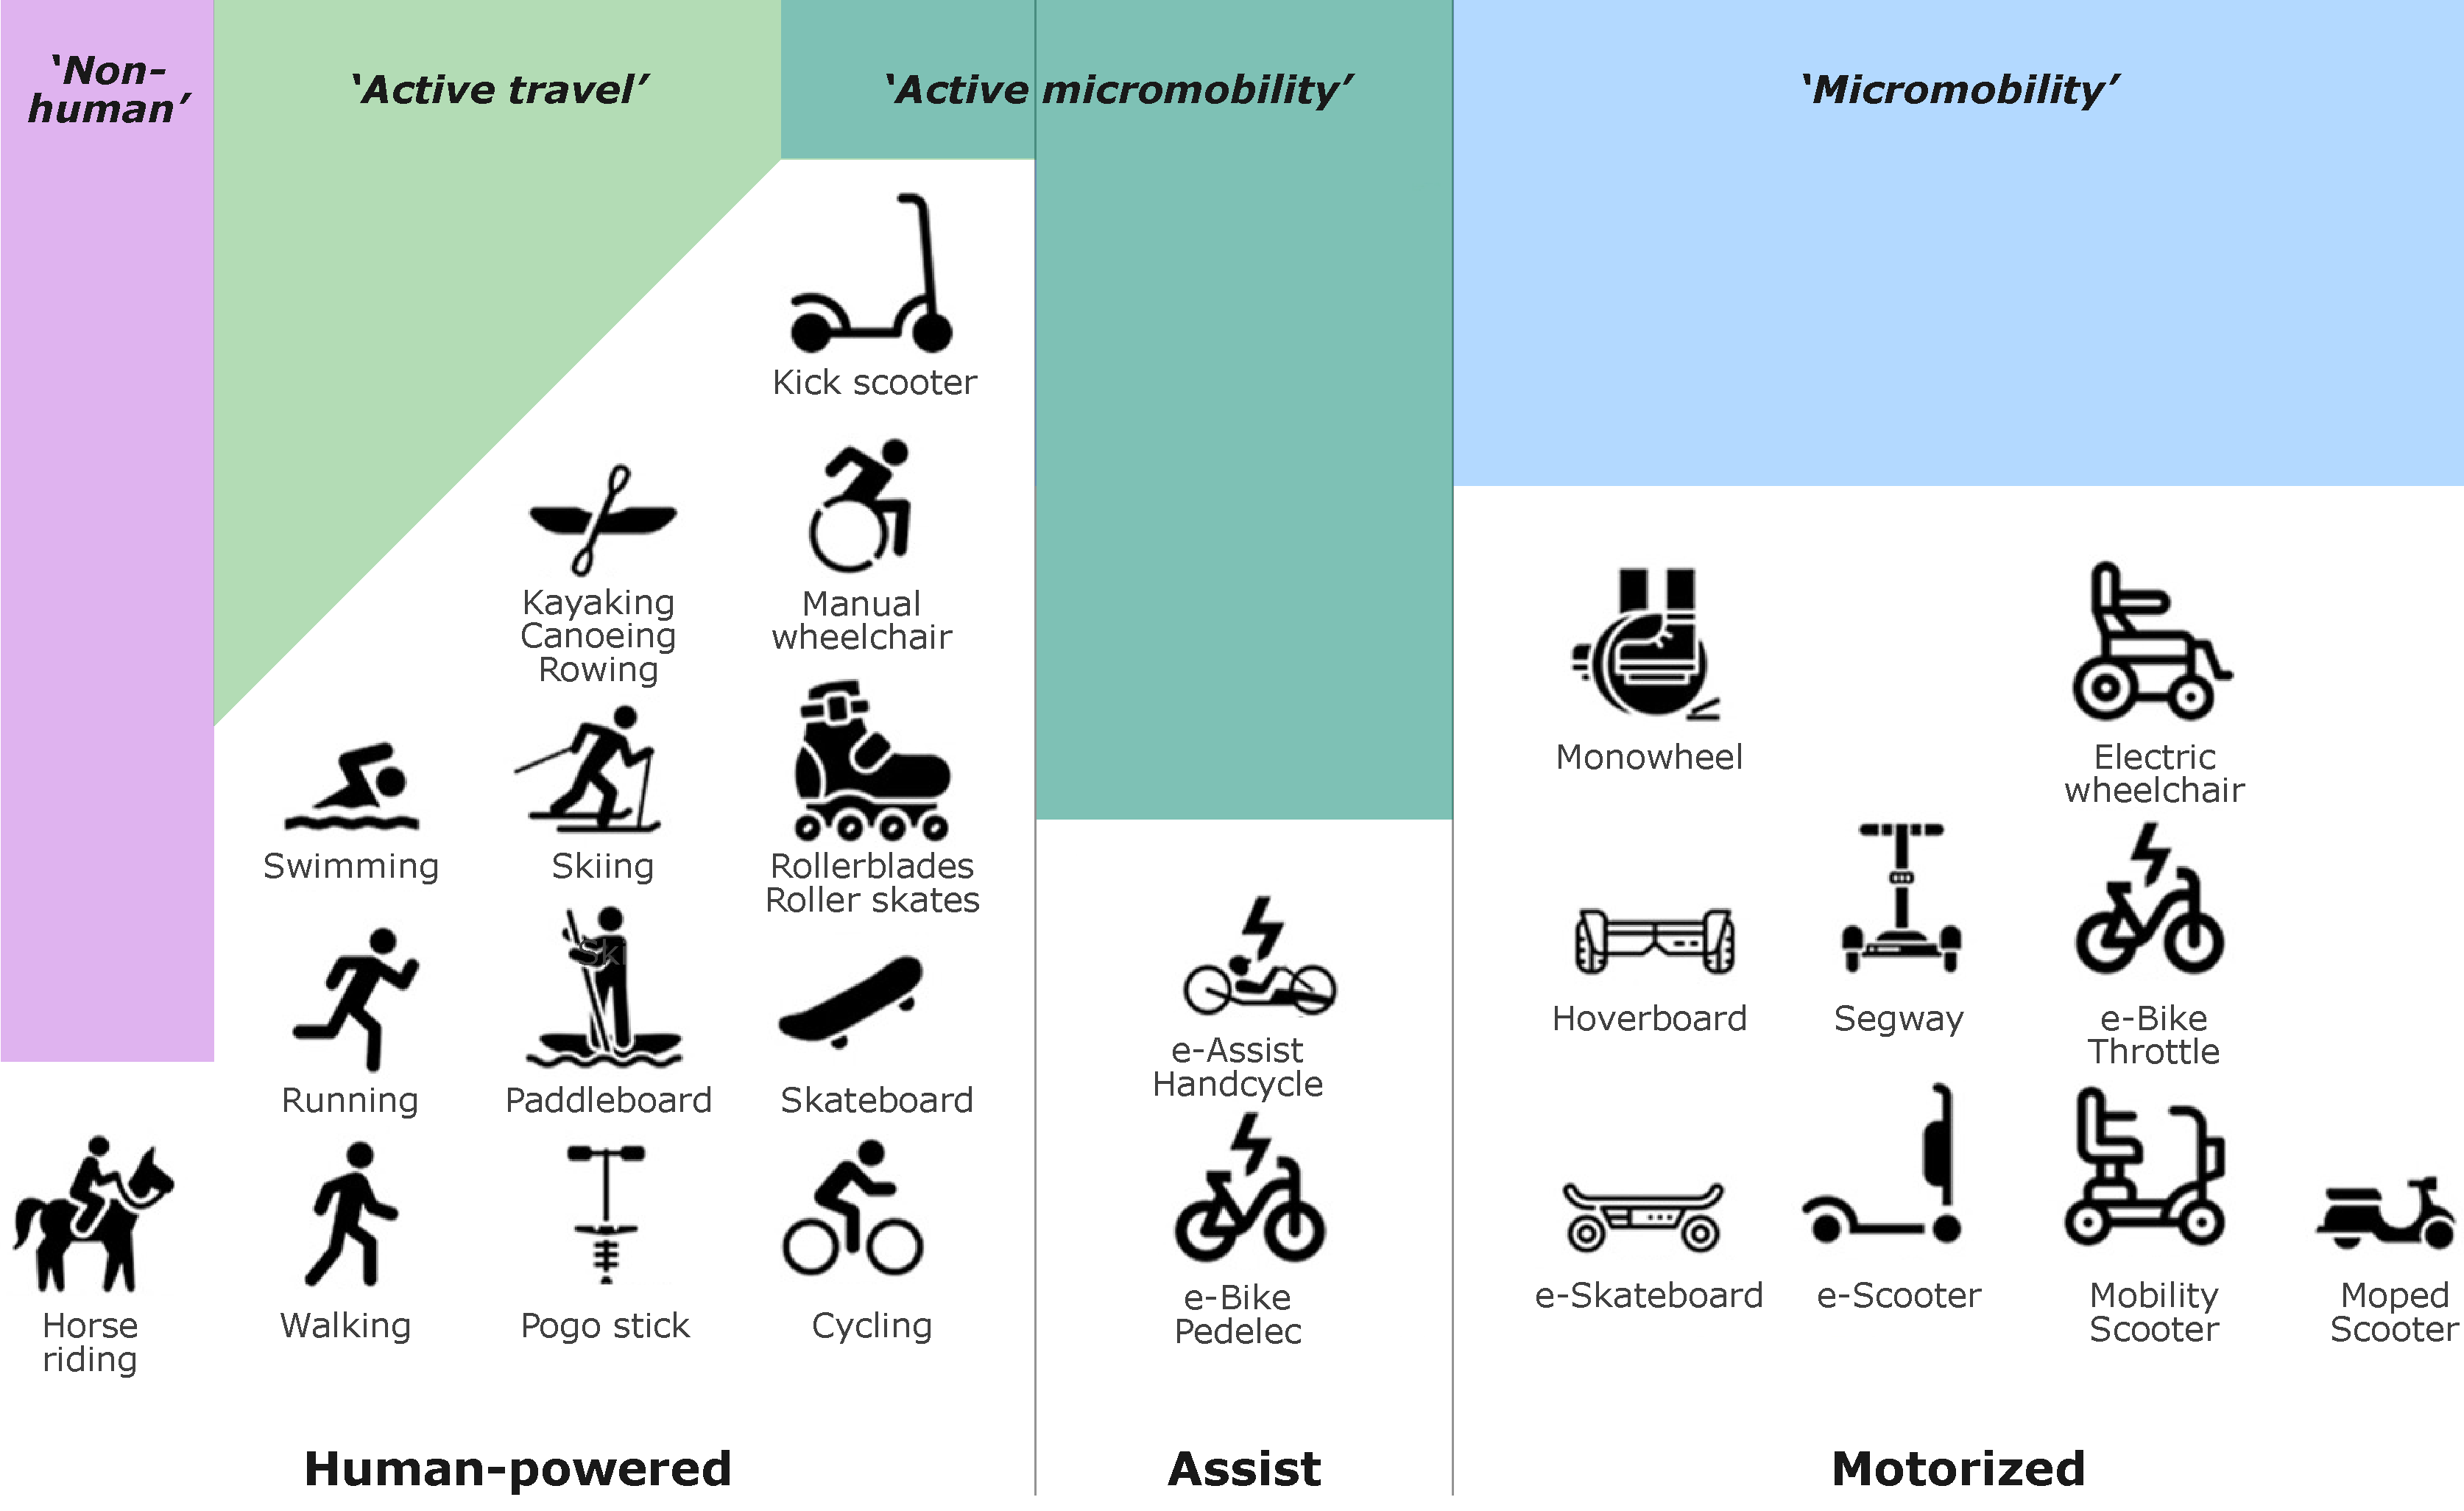
\includegraphics[width=1\columnwidth]{src/Figures/Chap-1/EN_Ecosysteme_micromobilite.pdf}}
        \vspace{5pt}
        \begin{flushright}\scriptsize{
        Source: \textcolor{blue}{\textcite[155]{cook_more_2022}}\index{Cook, Simon|pagebf}\index{Stevenson, Lorna|pagebf}\index{Aldred, Rachel|pagebf}\index{Kendall, Matt|pagebf}\index{Cohen, Tom|pagebf}
        \\
        Graphic adaptation: \textcolor{blue}{Dylan Moinse (2024)}
        }\end{flushright}
    \end{figure}

    % Contemporary History of e-Bike
In 1993, the Japanese motorcycle manufacturer \Marque{Yamaha Motor Company} introduced the first commercially successful electric bicycle, featuring a pedal-assist function (\textsl{Power Assist System}) and powered by a removable \acrshort{NiMH} battery \textcolor{blue}{\autocite[430]{bertoluzzo_development_2011}}\index{Bertoluzzo, Manuele|pagebf}\index{Buja, Giuseppe|pagebf}. This bicycle offers notable advantages over the traditional lead-acid battery, providing a lighter battery, less sensitive to ambient temperature variations, and with a longer lifespan. The pedal-assist system not only extended the battery's life but also made the user experience more intuitive. Because of these qualities, \textcolor{blue}{Noël} \textcolor{blue}{\textcite[25]{jouenne_quest-ce_2022}}\index{Jouenne, Noël|pagebf} describes the \acrshort{e-Bike} as an \Commas{electromechanical assisted bicycle} in his \acrfull{HDR} on the ethnology of the bicycle as a technical and social object, emphasizing the energy mix required for movement. From 2003, the electric bicycle benefited from the development and commercialization of \acrshort{Li-ion} batteries \textcolor{blue}{\autocite[6]{hung_review_2020}}\index{Hung, Nguyen Ba|pagebf}\index{Lim, Ocktaeck|pagebf}. In France, \acrshort{e-Bike} sales experienced spectacular growth, rising from 37,000 units sold in 2011 to 338,000 in 2018, reaching 738,000 in 2022, before a slight decrease to 671,000 products in 2023. These figures represent 43\% of total electric vehicle sales in 2023 \textcolor{blue}{\autocite{union_sport__cycle_chiffres_2024}}\index{Union Sport \& Cycle@\textsl{Union Sport \& Cycle}|pagebf}. Alongside \acrshort{e-Bike}, new forms of bicycles such as cargo bikes and tricycles have expanded the possibilities of electric bicycle use. These models facilitate not only long-distance travel or use by elderly or mobility-impaired individuals but also the transport of people and heavy goods. They thus open new perspectives for family travel, bike-taxi services, urban logistics, and self-employment. According to \textcolor{blue}{\textcite[24]{mason_global_2015}}\index{Mason, Jacob|pagebf}\index{Fulton, Lew|pagebf}\index{McDonald, Zane|pagebf}, the modal share of bicycles, stimulated by the growing popularity of \acrshort{e-Bike}, could reach 17\% by 2030 and 22\% by 2050 among OECD countries.%%Translated%%

% Contemporary History of TEP + Transition
Alongside the rise of the \acrshort{e-Bike}, the scooter makes a return to the forefront, first as a toy, and then gradually adopted by teenagers\footnote{~
    The spread of the modern scooter was facilitated by a major technical innovation that made it lighter, more durable, and more maneuverable thanks to the use of aluminum, a material that also made it foldable \textcolor{blue}{\autocite{arte_histoire_2014}}. In 1996, Swiss businessman \textcolor{blue}{Wim Ouboter} played a pivotal role in the evolution of the scooter. He founded his own company, \Marque{Micro Mobility Systems}, and by 1999, designed \Commas{micro-scooters}, combining the aesthetics of the scooter with wheels inspired by the \textsl{skateboard} \textcolor{blue}{\autocite{les_numeriques_futur_2015}}\index{Les Numériques@\textsl{Les Numériques}|pagebf}. Quickly, this model, marketed under the \Marque{Razor} brand, became a global phenomenon, reaching one million units sold in 2000 before the excitement waned. Despite this decline, the scooter maintained its status as a toy primarily intended for children. In the United States, it \Commas{invaded the cul-de-sacs of residential areas}, and the \textsl{Toy Association} named this model \Commas{Toy of the Year} in 2000 \textcolor{blue}{\autocite{bloomberg_citylab_man_2018}}. However, this enthusiasm quickly faded \textcolor{blue}{\autocite[25]{university_of_st_gallen_micro_2011}}\index{University of St. Gallen@\textsl{University of St. Gallen}|pagebf}. At the same time, the scooter evolved, being redeployed in a different context. A change in usage and customer base occurred: the reinforced scooter became a tool for a new sport, freestyle, inspired by BMX (\textsl{bicycle motocross}) and \textsl{skateboarding}. This sport, which involves performing acrobatic stunts (\textsl{tricks}), attracted a new generation of users, the \textsl{trottiriders} \textcolor{blue}{\autocite{micro-mobility_innovations_2018}}\index{Micro-mobility@\textsl{Micro-mobility}|pagebf}. Thus, the scooter gradually ceased to be seen as a mere toy and became a popular piece of equipment among teenagers and young adults, drawn to extreme sports and urban culture \textcolor{blue}{\autocite{ma_trott_histoire_2020}}.
} before undergoing a transformation through a modernized design and the integration of an electric battery. The man considered the \Commas{pioneer of the scooter revolution}, \textcolor{blue}{Wim Ouboter}, initiated this transformation based on his personal experience\footnote{~
    \textcolor{blue}{Wim Ouboter} relates that his interest in the scooter stemmed from his personal experience. As a child, he and his sister used old scooters, the latter being unable to ride a bicycle or ski due to a physical disability. However, it was at the age of 30 that the true revelation occurred. According to his account, the Swiss entrepreneur realized that his favorite sausage restaurant, located in Zurich, was too far to walk but not far enough to justify using a bike or car \textcolor{blue}{\autocite{ma_trott_histoire_2020}}.
} \textcolor{blue}{\autocite{ma_trott_histoire_2020}}\index{Ma Trott'@\textsl{Ma Trott'}|pagebf}. The scooter was rehabilitated with the creation of \Marque{Micro}, designed for what are termed \Commas{micro-distances}, situated between trips that are too long to walk and too short to use a car or a bike \textcolor{blue}{\autocite{oconnell_travel_2002}}\index{O'Connel, Dee|pagebf}. In line with the electrification of urban mobility in 2003, the Swiss entrepreneur expanded his range by developing electric models, still targeting an adult clientele \textcolor{blue}{\autocite{ma_trott_histoire_2020}}\index{Ma Trott'@\textsl{Ma Trott'}|pagebf}. But it was truly the launch of the \Marque{Xiaomi Mi Electric Scooter} (M365) in 2016, first in China, that disrupted the market. Released in Europe in 2018, the \acrshort{PeS} became a global success thanks to its affordable price and ergonomic design. Massively adopted for personal use, it also became a benchmark model for a multitude of shared scooter fleets. In France, the popularity of the \acrshort{PeS} was immediate: according to the barometer of the \acrfull{FP2M}, sales started at 233,000 units in 2018, rose to 478,800 units the following year, and reached 678,000 units in 2023 \textcolor{blue}{\autocites[1]{fp2m_barometre_2021}[1]{fp2m_ventes_2023}}\index{FP2M@\textsl{FP2M}|pagebf}. These numbers now surpass \acrshort{e-Bike} sales, which are also expanding. The example of the scooter, whether human-powered or electric, and that of the \acrshort{e-Bike}, folding or standard, perfectly illustrate the diversification of mobility modes in urban areas, both in forms accessible for purchase and rental.%%Translated%%

% 1.2.2.2.
\needspace{1\baselineskip} % Reserve space
\subsubsection*{The Sharing Economy in Service of Shared Mobility
    \label{chap1:velo-micromobilite-innovations-partage}
    }

    % Self-service with station - History 1
The genesis of \acrshort{PBS} lies within the history of social movements that led to the return of bicycles to cities \textcolor{blue}{\autocite[23]{hure_mobilites_2019}}\index{Huré, Maxime|pagebf}. The idea of a \Commas{smart bike} shared in public space, accessible to all without the need for personal acquisition, first found its applications in 1965 thanks to a Dutch anarchist collective, \textsl{Provo}. As part of their fifth \Commas{provocation} (\textsl{Witte Fietsenplan}) and ahead of the 1966 municipal elections, this protest and libertarian movement made available to the citizens of Amsterdam about fifty white-painted bicycles, freely placed on the streets, with the goal of freeing the city from urban congestion\footnote{~
    The \textsl{Provo} group advocated for a municipal initiative to provide the population with 10,000 free bicycles, self-managed by a participatory system. In protest against the municipality's refusal of their project, the collective included a list of voters and relaunched about a hundred abandoned bicycles, repairing and painting them white \textcolor{blue}{\autocite[29]{hure_mobilites_2019}}\index{Huré, Maxime|pagebf}.
} \textcolor{blue}{\autocites[6]{smart_provo_2012}{demain_la_ville_doit-velib_2018}}\index{Smart, Alan|pagebf}\index{Demain La Ville@\textsl{Demain La Ville}|pagebf}. Although pioneering, this form of action remained illegal according to public authorities, yet it gave rise to the first generation of \acrshort{PBS}, based on a free system \textcolor{blue}{\autocite[160]{shaheen_bikesharing_2010}}\index{Shaheen, Susan~A.|pagebf}\index{Guzman, Stacey|pagebf}\index{Zhang, Hua|pagebf}. La Rochelle is often recognized as the first city to institutionalize such a system in 1976 with its \textsl{municipal bicycles}, also called \textsl{Yellow Bikes}, a fleet of 350 bikes spread over three rental points\footnote{~
    The very visible experience of the municipal system in La Rochelle raises the question of the transformations in public urban action regarding mobility, previously heavily dependent on state services, shifting from state dirigisme to a regulatory state that remains the primary funder of this project. With its 300 \acrshort{PBS}, the mayor at the time, \textcolor{blue}{Michel Crépeau}, aimed to \Commas{normalize} the use of bicycles in the city. This policy set up a restricted access area, limited to the interior of the old fortress, and hours, from 8 a.m. to 8 p.m., with system regulation dependent on citizen participation \textcolor{blue}{\autocite[31]{hure_mobilites_2019}}\index{Huré, Maxime|pagebf}. Such a project, inaugurated six months before the municipal elections, allowed the mayor to build international recognition and legitimize a new urban policy for the rehabilitation of the city center, already constructing an early form of political and territorial marketing through these mobility services \textcolor{blue}{\autocite[31]{hure_mobilites_2019}}\index{Huré, Maxime|pagebf}. The following year, a second fleet of 100 free \acrshort{PBS} was established, funded through private sponsorship based on an advertising model. This initiative marked a turning point, as the use of advertising gradually became a central mode of financing for \acrshort{PBS} systems \textcolor{blue}{\autocite[32-35]{fleury_mobilites_2022}}\index{Huré, Maxime|pagebf}\index{Fleury, Antoine|pagebf}\index{Frétigny, Jean-Baptiste|pagebf}\index{Kanellopoulou, Dimitra|pagebf}.
}. This model inspired other initiatives, such as the one launched in Cambridge in 1993, and helped stabilize the commercial architecture of shared mobility as it is practiced today. Finally, the mechanisms and symbolic values of \acrshort{PBS} are largely inspired by those of the supermarket cart, as noted by \textcolor{blue}{Maxime} \textcolor{blue}{Maxime} \textcolor{blue}{\textcite[40]{hure_mobilites_2019}}\index{Huré, Maxime|pagebf}. Copenhagen marked a decisive step between 1989 and 1995 with the introduction of \textsl{Bycyklen}, a system utilizing the coin-deposit mechanism and bike stands. This system, considered the second generation of \acrshort{PBS}, was adopted in Europe and the United States, but problems of theft related to user anonymity persisted\footnote{~
    A notable alternative to the classic \acrshort{PBS} model is represented by the \textsl{Call a Bike} service, deployed in several German cities, starting with Munich in 2000. This system operates on a different principle: the bike, locked in the public space with a lock, can be borrowed and returned freely. Access to the bike requires contacting a dedicated service, allowing users to obtain the lock code for a fee. This system offers two modes of operation: \textsl{Call a Bike FLEX}, without stations, and \textsl{Call a bike FIX}, with stations \textcolor{blue}{\autocite[18]{6t-bureau_de_recherche_etude_2018}}. At the time, \textsl{Deutsche Bahn} considered deploying this system in about a hundred stations on the Intercités express network to promote intermodality.
} \textcolor{blue}{\autocite[160]{shaheen_bikesharing_2010}}\index{Shaheen, Susan~A.|pagebf}\index{Guzman, Stacey|pagebf}\index{Zhang, Hua|pagebf}. The third generation, embodied by the \textsl{Vélo à la carte} of Rennes in 1998, introduced identification and reservation technologies. This computerized system relies on kiosks, personal cards, and later mobile phones, enabling a \textsl{check-in} and \textsl{check-out} of the bike \textcolor{blue}{\autocite[8]{nlc_micromobility_2019}}\index{NLC@\textsl{NLC}|pagebf}.%%Translated%%

% Figure VLS map France
\begin{carte}[h!]\vspace*{4pt}
    \caption{Location and evolution of station-based bike-sharing services in France, in 2018.}
    \label{fig-chap1:carte-vls-france}
    \centerline{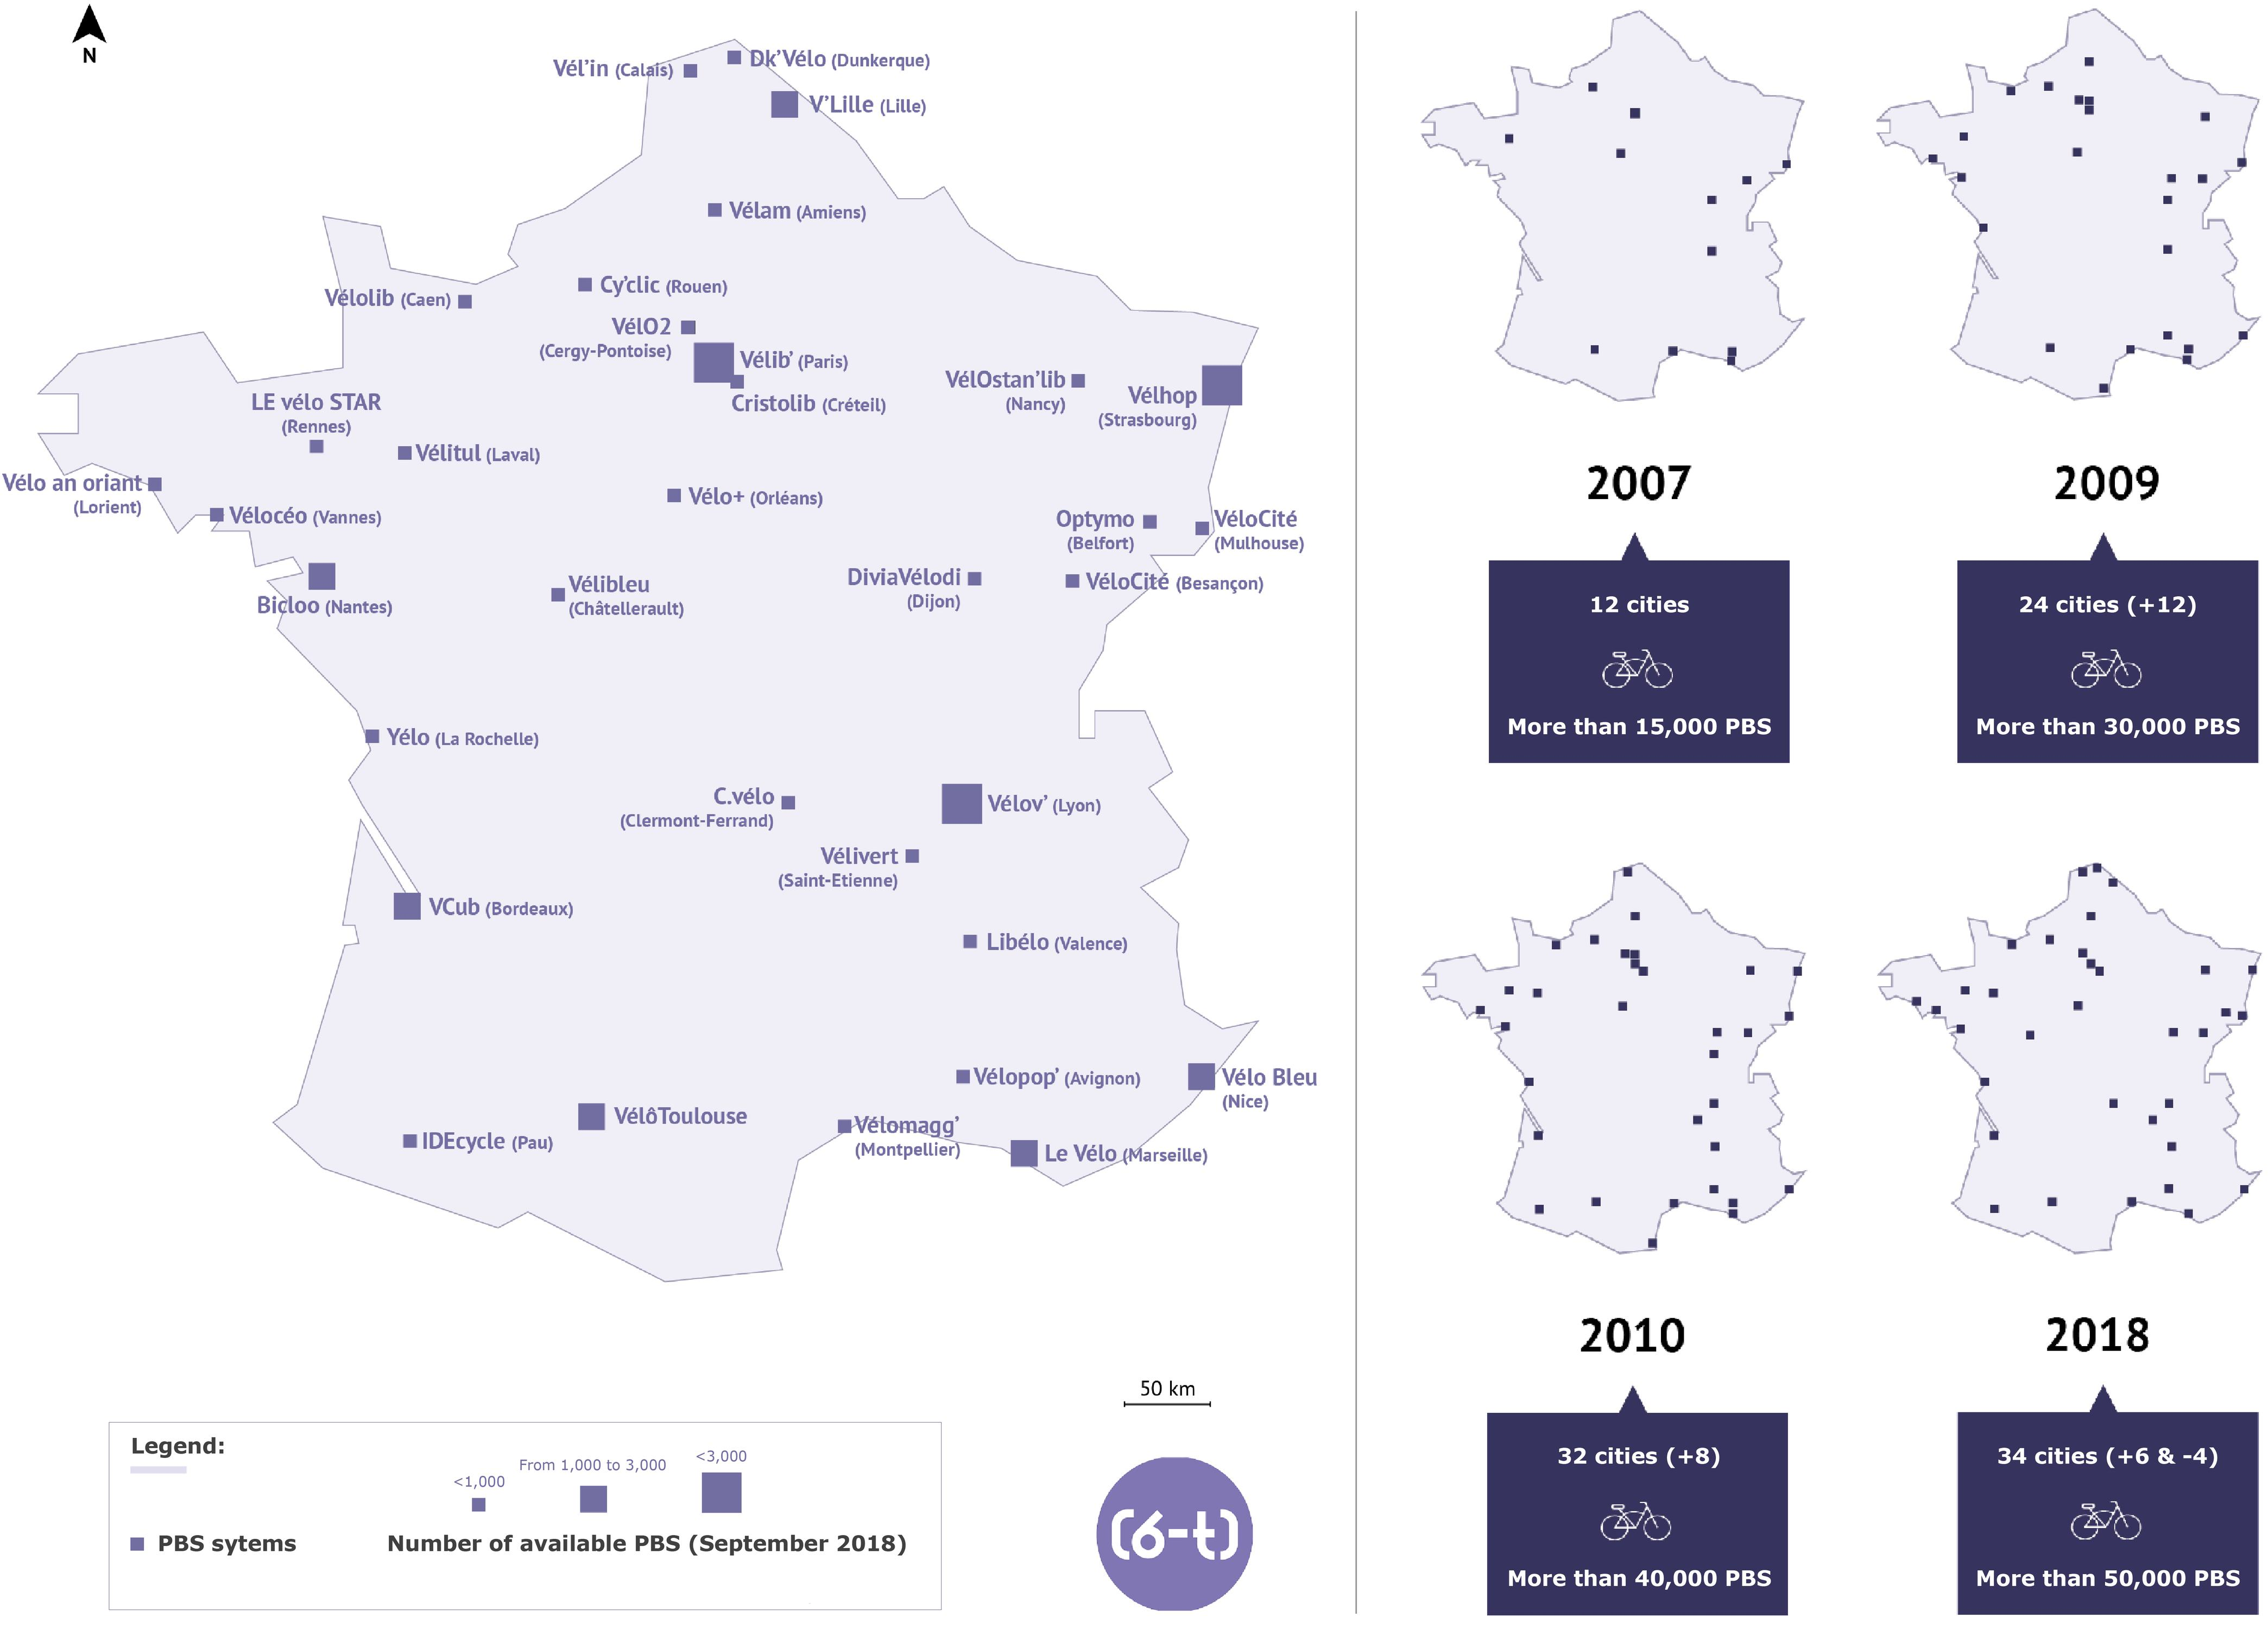
\includegraphics[width=1\columnwidth]{src/Figures/Chap-1/EN_Carte_VLS_France.jpg}}
    \vspace{5pt}
    \begin{flushright}\scriptsize{
    Source: \textcolor{blue}{\textcite{6t-bureau_de_recherche_lechappee_2018}}\index{Bureau de recherche 6t@\textsl{Bureau de recherche 6t}|pagebf}
    }\end{flushright}
\end{carte}

% Self-service with station - History 2
These innovations, combined with a pricing model based on time intervals, have become the international standard for \acrshort{PBS} systems \textcolor{blue}{\autocite[162]{shaheen_bikesharing_2010}}\index{Shaheen, Susan~A.|pagebf}\index{Guzman, Stacey|pagebf}\index{Zhang, Hua|pagebf}. However, it is Lyon, with \textsl{Vélo'v} in 2005, and Paris, with \textsl{Vélib'} in 2007, that popularized this model worldwide. These services became the benchmarks for \acrshort{PBS}, enabling France to take the lead in this area: by 2010, the country had 24 \acrshort{PBS} systems, with a total fleet of 36,000 bikes and 3,000 stations \textcolor{blue}{\autocite[161]{shaheen_bikesharing_2010}}\index{Shaheen, Susan~A.|pagebf}\index{Guzman, Stacey|pagebf}\index{Zhang, Hua|pagebf}, reaching 34 urban areas by 2018 (see \hyperref[fig-chap1:carte-vls-france]{Map~\ref{fig-chap1:carte-vls-france}}, page~\pageref{fig-chap1:carte-vls-france}). It is at the turn of this decade that the experiences of \acrshort{PBS} systems began to reveal a dominant management model: the \acrfull{PPP} \textcolor{blue}{\autocite[5]{hure_entre_2014}}\index{Huré, Maxime|pagebf}. More recently, a fourth generation has emerged, integrating \acrshort{e-Bike} for self-service, optimized locking mechanisms, touch interfaces, and interconnection with public transport systems \textcolor{blue}{\autocite[162]{shaheen_bikesharing_2010}}\index{Shaheen, Susan~A.|pagebf}\index{Guzman, Stacey|pagebf}\index{Zhang, Hua|pagebf}. It should be noted that while these initiatives are mostly the result of local or intercommunal projects led primarily by the largest urban areas \textcolor{blue}{\autocites[18]{fishman_bike_2013}[6]{ricci_bike_2015}}\index{Fishman, Elliot|pagebf}\index{Washington, Simon|pagebf}\index{Haworth, Narelle|pagebf}\index{Ricci, Miriam|pagebf}, their deployment remains marginal at the regional or national level\footnote{~
    Among these exceptions, we cannot avoid mentioning the Dutch system \textsl{OV-fiets}, literally translated as \textsl{public transport bikes}, integrated into the national railway network. Created in 2004 by an association, this \acrshort{PBS} system was taken over, starting in 2008, by the Dutch national railway company, \acrfull{NS} \textcolor{blue}{\autocites[151]{ploeger_sociotechnical_2020}[157]{waes_why_2020}}\index{Ploeger, Jan|pagebf}\index{Oldenziel, Ruth|pagebf}\index{Waes, Arnoud van|pagebf}\index{Farla, Jacco|pagebf}\index{Raven, Rob|pagebf}. Today, this mobility service covers 300 stations located near train stations and metro stops, with a fleet of 22,000 bikes. Its specificity lies in the fact that the rental occurs on a daily basis and requires that the bike be returned to the same station where it was borrowed \textcolor{blue}{\autocite[9]{ploeger_sociotechnical_2020}}\index{Caletrío, Javier|pagebf}, following a loop model, \textsl{2-way} type \textcolor{blue}{\autocite[13]{mangeart_vehicules_2022}}\index{Mangeart, Timothée|pagebf}\index{Bouteuil, Virginie|pagebf}.
} \textcolor{blue}{\autocite[225]{dauncey_french_2012}}\index{Dauncey, Hugh|pagebf}. In August 2022, according to the platform \textsl{The Meddin Bike-sharing World Map}\footnote{~
    \url{https://bikesharingworldmap.com}
}, which records and updates all shared mobility systems worldwide, 1,212 urban areas have \acrshort{PBS} services \textcolor{blue}{\autocite[7]{the_meddin_bike-sharing_world_map_meddin_2022}}\index{The Meddin Bike-sharing World Map@\textsl{The Meddin Bike-sharing World Map}|pagebf}, with the largest ones all located in China (see \hyperref[fig-chap1:carte-vls-monde]{Map~\ref{fig-chap1:carte-vls-monde}}, page~\pageref{fig-chap1:carte-vls-monde}). In addition to these, 80 so-called \Commas{hybrid} systems have emerged, combining a fleet of \acrshort{PBS} and a fleet of \acrfull{DBS}.%%Translated%%

% Figure VLS world map
\begin{carte}[h!]\vspace*{4pt}
    \caption{Location of major station-based bike-sharing services worldwide, in 2021.}
    \label{fig-chap1:carte-vls-monde}
    \centerline{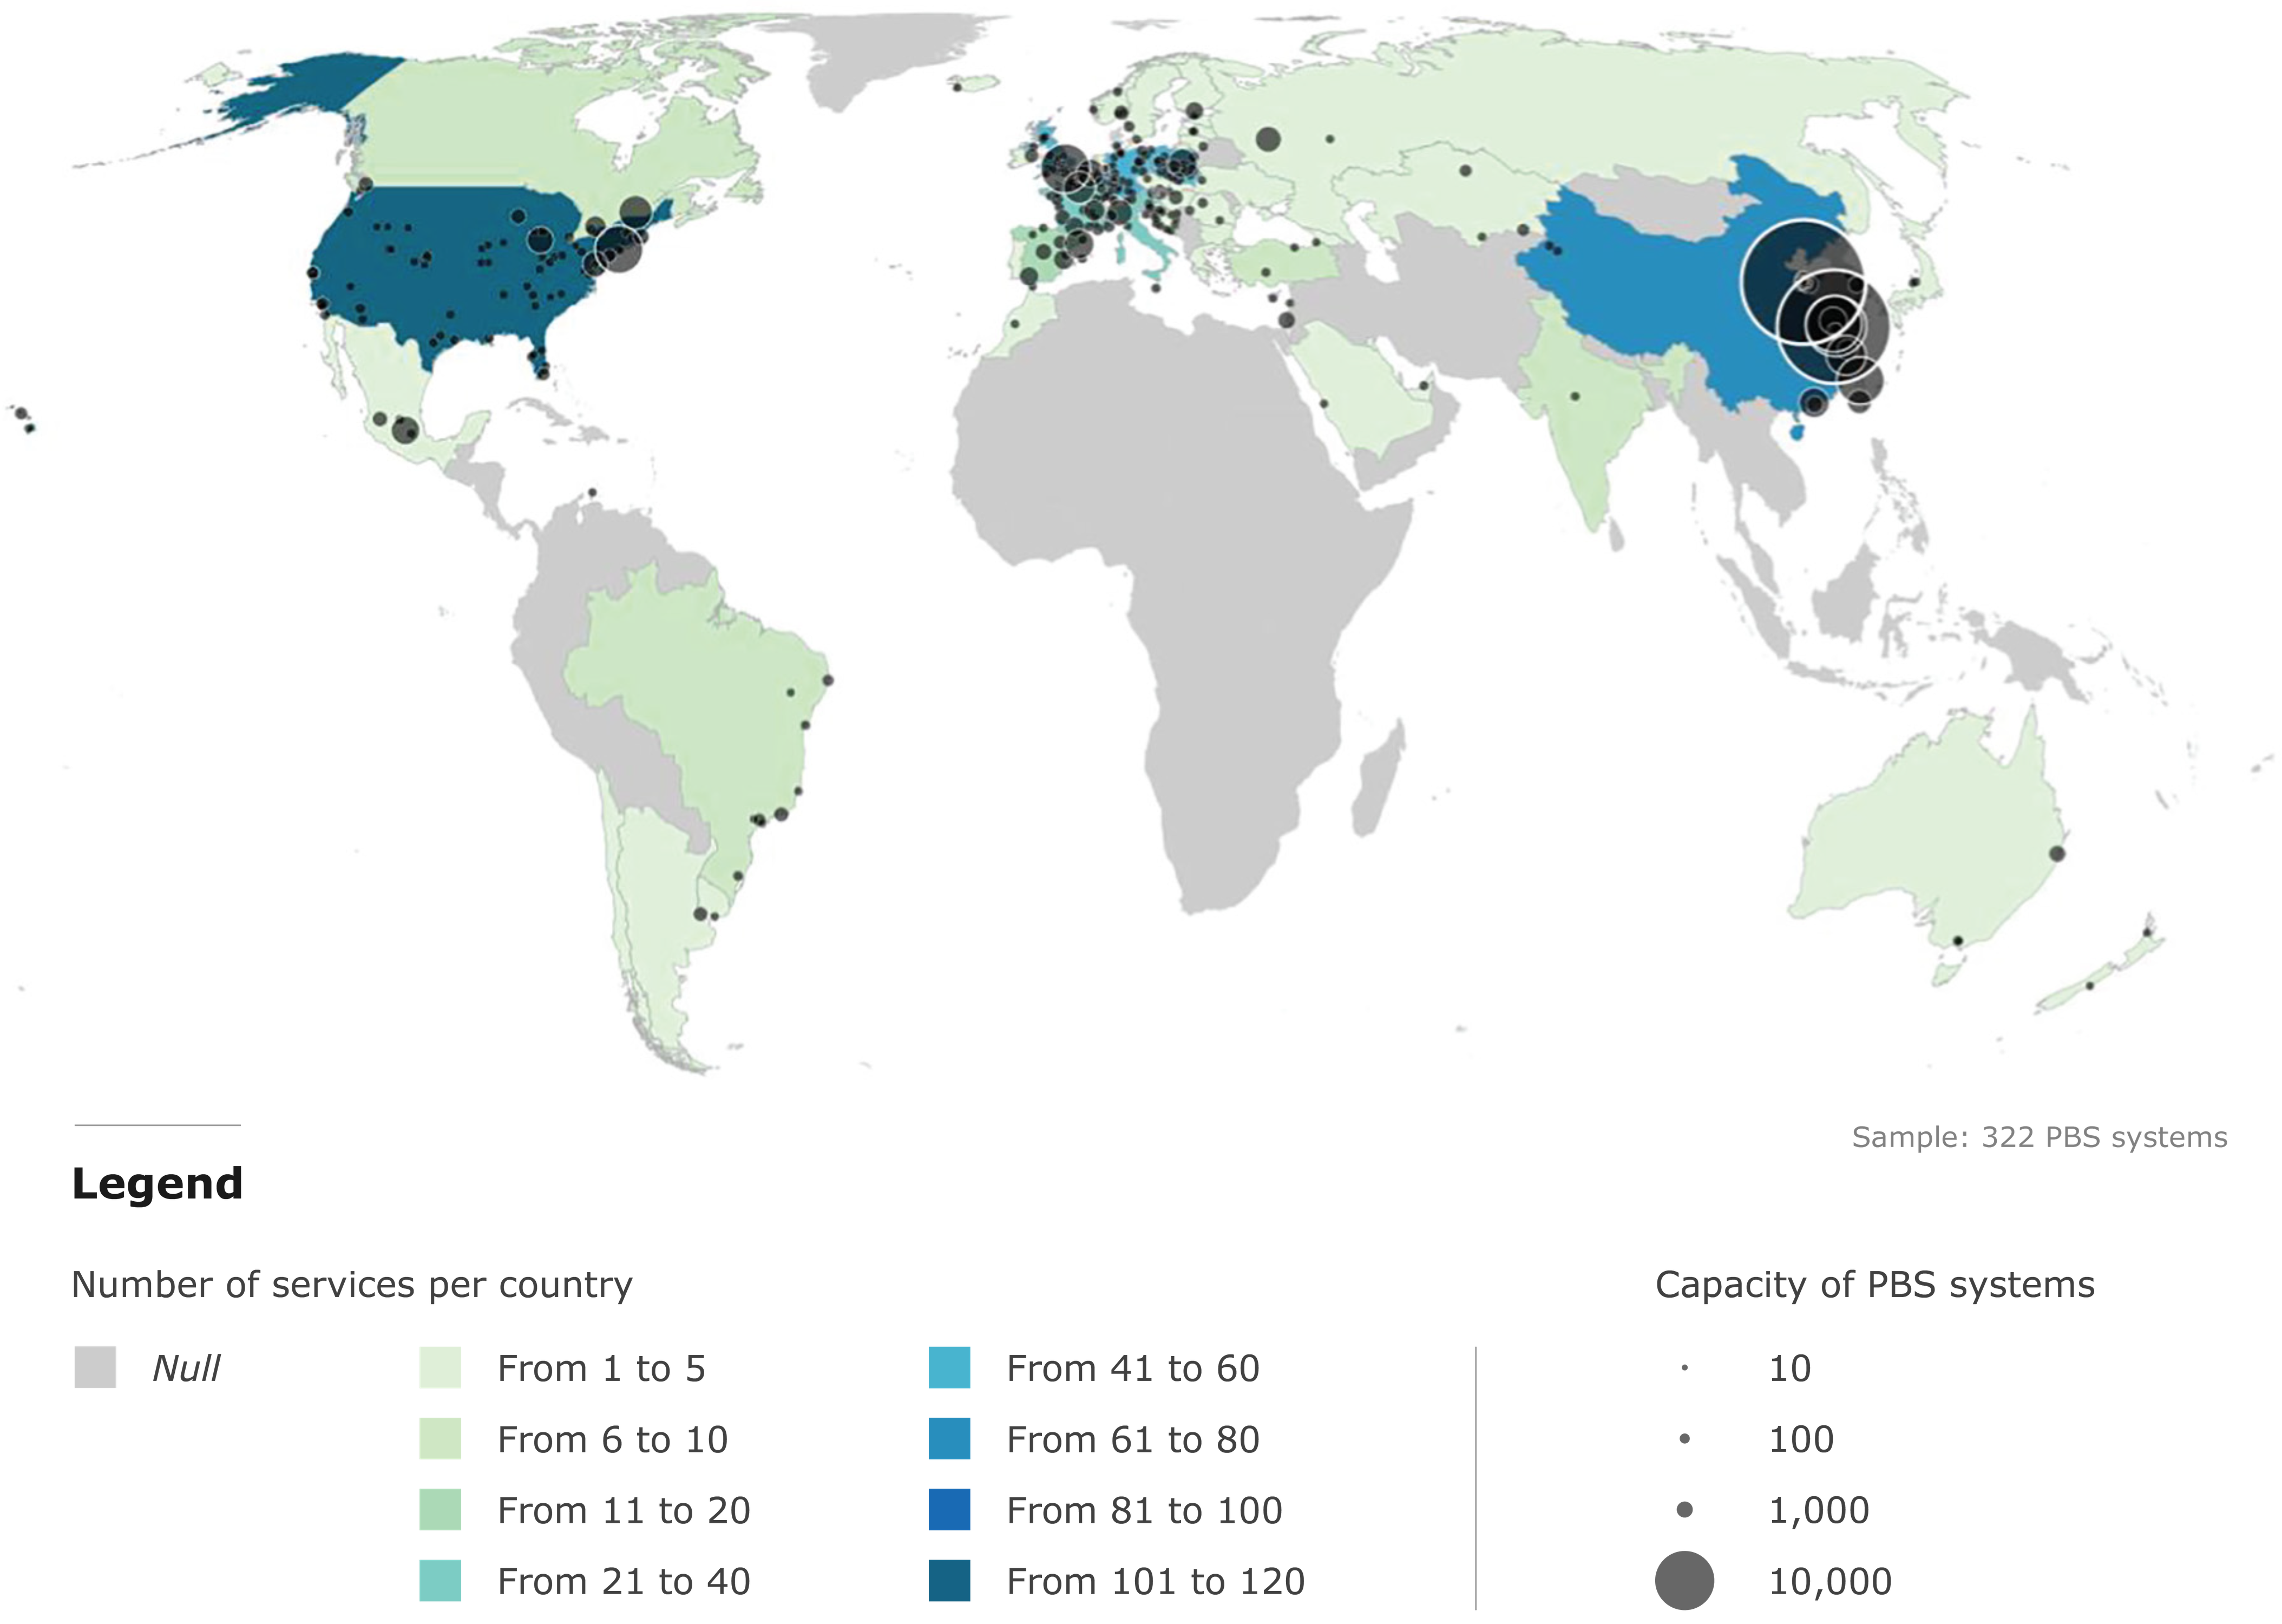
\includegraphics[width=1\columnwidth]{src/Figures/Chap-1/EN_Carte_VLS_monde.png}}
    \vspace{5pt}
    \begin{flushright}\scriptsize{
    Source: \textcolor{blue}{\textcite{todd_global_2021}}\index{Todd, James|pagebf}\index{O'Brien, Oliver|pagebf}\index{Cheshire, James|pagebf}
    \\
    Translation: \textcolor{blue}{Dylan Moinse (2024)}
    }\end{flushright}
\end{carte}

% VFF
While the experience of the \textsl{White Bikes}, \textsl{Call a Bike}, and successive generations of \acrshort{PBS} systems can be seen as the precursors to \acrshort{DBS} systems, their current form truly emerged in China in 2014. That year, \textcolor{blue}{Dai Wei}, a student in Beijing, along with his friends, came up with the idea of a shared bike system designed to facilitate their movement on campus. They founded the startup \Marque{Ofo} after experimenting with bike sharing on their campus \textcolor{blue}{\autocite[10]{nlc_micromobility_2019}}\index{NLC@\textsl{NLC}|pagebf}. This project quickly gained financial support from the Chinese \acrshort{RHS} company \Marque{Didi} \textcolor{blue}{\autocite[18]{6t-bureau_de_recherche_etude_2018}}\index{Bureau de recherche 6t@\textsl{Bureau de recherche 6t}|pagebf}. The service expanded to several Chinese cities before going international. Many Asian \Commas{bike unicorns}\footnote{~
    In 2013, U.S. investor \textcolor{blue}{Aileen Lee} coined the term \Commas{unicorn} to refer to the most highly valued startups in Silicon Valley, California. The mythical animal symbolizes rarity, miracles, and fantasy \textcolor{blue}{\autocite{benner_unicorn_2015}}\index{Benner, Katie|pagebf}. Essentially, it describes a \Commas{\textsl{new technology startup founded less than ten years ago, valued at least one billion dollars before going public.}} \textcolor{blue}{\autocite{chambre_de_commerce_et_dindustrie_licornes_2019}}\index{Chambre de commerce et d'industrie@\textsl{Chambre de commerce et d'industrie}|pagebf}.
} specializing in station-free shared bikes, called \Commas{dockless} sharing system (or \textsl{free-floating}), emerged and expanded their activities to France starting in the fall of 2017. For example, \Marque{Gobee.bike} first deployed its bikes in Lille, followed by Paris a few days later. Within just a few months, five \acrshort{DBS} operators were active in Paris by the end of 2017. Less than a year later, seven \acrshort{DBS} services expanded to eight French cities, with a total fleet of around 15,000 bikes, representing 20\% of shared bikes in the country \textcolor{blue}{\autocite[23]{6t-bureau_de_recherche_etude_2018}}\index{Bureau de recherche 6t@\textsl{Bureau de recherche 6t}|pagebf}. Meanwhile, the two Chinese giants of the sector, \Marque{Ofo} and \Marque{Mobike}, expanded to the 30 largest cities in China, gathering over 200 million users, and also reached 21 other countries \textcolor{blue}{\autocite[22, 91]{kang_university_2020}}\index{Kang, Wei|pagebf}\index{Aguiléra, Anne|pagebf}\index{Rallet, Alain|pagebf}.%%Translated%%

% TEFF
Beyond the description of the vehicle itself, it is primarily the dockless sharing operational model that fuels the discussion on expanding mobility options. Shortly after the deployment of fleets of \acrshort{DBS}, whether mechanical or electric, new services emerge, notably those related to \acrfull{DESS}. Its rise began in 2017 with the creation of the American company \Marque{Bird} by \textcolor{blue}{Travis VanderZanden}, a former executive at \Marque{Lyft} and \Marque{Uber} \textcolor{blue}{\autocite[13]{nlc_micromobility_2019}}\index{NLC@\textsl{NLC}|pagebf}. This project focuses on the revival of the electric scooter, which had been reintroduced a few years earlier \textcolor{blue}{\autocite{easy_electric_life_free_2020}}\index{Easy Electric Life@\textsl{Easy Electric Life}|pagebf}. In France, \acrshort{DESS} services emerged in the summer of 2018, quickly becoming emblematic, alongside \acrshort{DBS}, of the rise of shared mobility \textcolor{blue}{\autocite[1]{bortoli_consequential_2020}}\index{Bortoli, Anne de|pagebf}\index{Christoforou, Zoi|pagebf}. Although shared electric scooter and car services already existed in Europe, the adoption and deployment speed of \acrshort{DESS} systems was unprecedented. For instance, \Marque{Bird} quickly reached \Commas{unicorn} status, and other companies such as \Marque{Lime} (formerly \Marque{LimeBike}) or \Marque{Spin}, originally specialized in \acrshort{DBS}, followed the model in 2018 \textcolor{blue}{\autocite[4]{clewlow_micro-mobility_2018}}\index{Clewlow, Regina|pagebf}. Described as the \Commas{latest form of the Uberization of urban mobility} \textcolor{blue}{\autocite[1]{boffi_extrait_2019}}\index{Boffi, Nicolas|pagebf}, \acrshort{DBS} and \acrshort{DESS} services have set records in terms of diffusion and modal adoption internationally. In Paris, \textcolor{blue}{\textcite[146]{6t-bureau_de_recherche_usages_2019}}\index{Bureau de recherche 6t@\textsl{Bureau de recherche 6t}|pagebf} estimates that, just one year after its launch, \acrshort{DESS} achieved at least a modal share equivalent to that of the \acrshort{PBS} \textsl{Vélib’}, three years after its launch, with an estimate between 0.8\% and 2.2\% of internal trips. In the U.S. and Canada, 39 million \acrshort{DESS} trips were recorded in the first year of service, a number that will double by 2023, despite the COVID-19 health crisis. North American \acrshort{DESS} systems then represent 44\% of shared bike or scooter trips on the continent, a proportion that rises to 49\% in the U.S. \textcolor{blue}{\autocites[10]{nacto_shared_2019}[10]{nacto_shared_2020}[3-5]{nacto_shared_2024}}\index{NACTO@\textsl{NACTO}|pagebf}. One key element, however, distinguishes dockless sharing mobility systems from station-based ones: their geographical distribution. While \acrshort{PBS} services are mainly concentrated in large metropolitan areas, \acrshort{DBS} and \acrshort{DESS} services are deployed in relatively less dense areas.%%Translated%%

% Technologies
Shared mobility, whether in the form of bicycles or scooters, mechanical or electric, is characterized by a common denominator: it frees the user from the costs of acquisition, maintenance, and the responsibilities associated with vehicle ownership \textcolor{blue}{\autocite[44]{mathew_analysis_2019}}\index{Mathew, Jijo|pagebf}\index{Liu, Mingmin|pagebf}\index{Li, Howell|pagebf}\index{Seeder, Sonya|pagebf}\index{Bullock, Darcy|pagebf}. This offering, although diverse, fits into a dynamic of complementarity, but also competition with traditional vehicles. It emerged thanks to a favorable technological context, marked by the commercialization and democratization of recent innovations. First and foremost, the massive diffusion of \textsl{smartphones}\footnote{~
    The \textsl{smartphone}, conceived in 1992, marked a major technological turning point, but it was truly popularized with the release of the \Marque{Iphone} in 2007. By 2008, the \Marque{Iphone 3G} allowed access to the 3G cellular data network, was equipped with GPS functionality, and introduced the use of apps updated through an online store \textcolor{blue}{\autocite{les_numeriques_2007_2014}}\index{Les Numériques@\textsl{Les Numériques}|pagebf}. These advancements profoundly transformed individual behaviors by integrating the \textsl{smartphone} into everyday uses, such as mobile payments (M-payment) or reading \textsl{flashcodes} (\textsl{QR codes}) \textcolor{blue}{\autocites[279]{chaix_paiement_2013}[21]{ben_jaddi_m-paiement_2018}}\index{Chaix, Laetitia|pagebf}\index{Ben Jaddi, Madja|pagebf}. This technological revolution provided fertile ground for the development of shared mobility services, which leverage the five components of the \Commas{\textsl{Internet} of things}, also known as \acrfull{IoT}, namely (i) objects, (ii) the mobile network, (iii) data, (iv) information, and (v) operational applications \textcolor{blue}{\autocite{iot_evolution_world_impact_2017}}\index{IoT Evolution World@\textsl{IoT Evolution World}|pagebf}. Moreover, the widespread adoption of \textsl{smartphones} opened up a huge potential market for these services. The device's democratization was rapid and global. For example, in the United States, the smartphone penetration rate rose from 35\% in 2011 to 77\% in 2018 \textcolor{blue}{\autocite[8]{clewlow_micro-mobility_2018}}\index{Clewlow, Regina|pagebf}. A similar dynamic was observed in France, where this rate went from 17\% in 2011 to 77\% in 2019 \textcolor{blue}{\autocite[28]{credoc_barometre_2019}}\index{CRÉDOC@\textsl{CRÉDOC}|pagebf}.
} enabled \acrfull{STP} to free themselves from the physical anchor of stations. This dematerialization facilitated the implementation of operational models summarized by the saying: \Commas{\textsl{arrive first, ask later}}\footnote{~
    The first generation of shared bike and scooter services, deployed between 2017 and 2020, was characterized by an audacious strategy adopted by operators. They would set up services on territories without prior authorization from local authorities or even informing them, taking advantage of the legal ambiguity surrounding these new mobility services \textcolor{blue}{\autocite{laker_welcome_2019}}\index{Laker, Laura|pagebf}. This tactic was to establish the services \textsl{de facto} before contacting local authorities, aiming to negotiate from a position of strength, thus reducing the necessary concessions \textcolor{blue}{\autocite[5]{lopez-escolano_mobilites_2019}}\index{López-Escolano, Carlos|pagebf}\index{Campos, Ángel Pueyo|pagebf}. The regulatory vacuum regarding the occupation of public space allowed these services to operate without formal agreements \textcolor{blue}{\autocite[5]{lopez-escolano_mobilites_2019}}\index{López-Escolano, Carlos|pagebf}\index{Campos, Ángel Pueyo|pagebf}. This situation led some cities to ban these services, primarily citing two main reasons: illegal occupation of public space and direct competition with existing public transport systems \textcolor{blue}{\autocite[63]{6t-bureau_de_recherche_livre_2019}}. However, these tactics have evolved today. This phase has been replaced by more collaborative approaches, allowing both public and private actors to mutually benefit from these services. Today, operating and regulatory charters govern the implementation of shared mobility services in most major European and North American cities, thus ending unilateral practices and laying the foundations for governance.
}, where operators often caught public authorities off guard. These authorities, historically regulators of urban transport and sometimes operators themselves of services such as \acrshort{PBS}, found themselves in a disadvantageous position against these disruptive actors. Besides the central role of \textsl{smartphones}, geolocation and geofencing also played a strategic role in the deployment of these mobility solutions. Thanks to these technologies, operators can track their fleets in real-time and establish virtual geographic barriers defining the operating areas. However, \acrshort{GPS} technology, with its limited accuracy of 3 to 10 meters depending on the urban environment \textcolor{blue}{\autocite{the_scooterist_dockless_2020}}\index{The Scooterist@\textsl{The Scooterist}|pagebf}, still constitutes a hindrance to fine management of shared vehicles, especially to distinguish between movement or parking on a sidewalk, roadway, or in restricted areas \textcolor{blue}{\autocite[96]{6t-bureau_de_recherche_livre_2019}}\index{Bureau de recherche 6t@\textsl{Bureau de recherche 6t}|pagebf}\footnote{~
    Currently, geolocation of dockless sharing vehicles allows detecting their entry or exit from defined areas, such as expanded parking zones or specific locations like public squares or parks. However, the precision offered by \acrshort{GPS} technology remains limited, not always meeting the expectations of local authorities, who sometimes overestimate its effectiveness as a management solution \textcolor{blue}{\autocite[123]{6t-bureau_de_recherche_livre_2019}}. In response to these limitations, some urban or transport authorities have introduced complementary solutions. These include requiring the user to scan a \textsl{QR code} located in a standardized parking area at the end of the trip, or photographing the parked vehicle as proof of compliance \textcolor{blue}{\autocite[96]{6t-bureau_de_recherche_livre_2019}}.
}. This landscape is expected to evolve with the full operation of the European satellite positioning system \textsl{Galileo}, initiated by the European Union. Partially operational since 2016, this system was finalized at the end of 2024 and is now accessible to the public with free accuracy of about one meter, and centimeter-level accuracy for paid services \textcolor{blue}{\autocite{futura_sciences_galileo_2019}}\index{Futura Sciences@\textsl{Futura Sciences}|pagebf}\index{CNES@\textsl{CNES}|pagebf}. This technological breakthrough opens new prospects for geofencing, not only to improve fleet management and accuracy but also to meet regulatory requirements, especially regarding the parking of shared vehicles.%%Translated%%

 % Semi-floating and Transition
In their \Commas{umbrella review} of shared vehicles, which is a synthesis of 29 existing literature reviews, \textcolor{blue}{\textcite[16]{mangeart_vehicules_2022}}\index{Mangeart, Timothée|pagebf}\index{Bouteuil, Virginie|pagebf} highlight the frequent lack of specific strategies adopted by local authorities regarding shared mobility services. The identified regulatory instruments range from restrictions, public funding, and in-kind benefits, such as the provision of parking spaces. This evolution in public governance is a marker of a profound transformation in the \Commas{socio-technical regime}, driven by the pressure of innovations \textcolor{blue}{\autocites[319]{canitez_pathways_2019}[4]{fryszman_smart_2019}}\index{Canitez, Fatih|pagebf}\index{Fryszman, Flavia|pagebf}\index{Denes Dos Santos Carstens, Danielle|pagebf}\index{Kindl da Cunha, Sieglinde|pagebf}. One of the notable evolutions concerns the organization of \Commas{semi-floating} fleets or \Commas{semi-dockless}, taking the form of either physical or dematerialized stations \textcolor{blue}{\autocite[121]{6t-bureau_de_recherche_livre_2019}}\index{Bureau de recherche 6t@\textsl{Bureau de recherche 6t}|pagebf}. This reflection on \textsl{smartparking} aims to reduce negative externalities, such as inconvenient parking on pedestrian spaces \textcolor{blue}{\autocite[13]{zou_exploratory_2020}}\index{Zhou, Zhenpeng|pagebf}\index{Younes, Hannah|pagebf}\index{Erdoğan, Sevgi|pagebf}\index{Wu, Jiahui|pagebf}. In Paris, for example, the municipality announced in March 2019 that fees imposed on operators would be used to fund 2,500 parking spaces dedicated to \acrshort{DBS} and \acrshort{DESS}\footnote{~
    Parking spaces dedicated to \textsl{dockless sharing} vehicles are often marked on the ground with a specific logo, frequently replacing a car parking space \textcolor{blue}{\autocite{livonniere_trottinettes_2019}}\index{Livonnière, Stanislas de|pagebf}. These spaces are typically sized to accommodate six \acrshort{DESS}, for example \textcolor{blue}{\autocite{burban_trottinettes_2019}}\index{Burban, Thibault|pagebf}. This measure makes sense with the municipal decree of July 30, 2019, which prohibits the parking of \acrshort{DBS} and \acrshort{DESS} on sidewalks. The text specifies: \Commas{\textsl{Considering that, under these conditions, it is necessary to organize the parking of these vehicles to ensure pedestrian safety and guarantee good walking conditions, restricting parking possibilities to only those places adapted to their geometric and functional characteristics.}} \textcolor{blue}{\autocite[3151]{ville_de_paris_bulletin_2019}}. This initiative complements an application and strategic reinterpretation of Article 52 of the 2019 \acrfull{LOM}, which states that parking spaces for cars located within five meters of pedestrian crossings will be neutralized before 2027 to ensure better visibility for pedestrians \textcolor{blue}{\autocite[42]{gart_loi_2020}}. To date, around 2,500 reserved parking spaces have been created in the capital, representing a total of 15,000 spaces for \acrshort{DBS} and \acrshort{DESS}.
} \textcolor{blue}{\autocites[3151]{ville_de_paris_bulletin_2019}[90]{6t-bureau_de_recherche_livre_2019}}\index{Bureau de recherche 6t@\textsl{Bureau de recherche 6t}|pagebf}\index{Ville de Paris@\textsl{Ville de Paris}|pagebf}. Reminiscent of the pioneering operation model of the Danish \acrshort{DBS} company \Marque{Donkey Republic}\footnote{~
    Facing competition from massive Asian and North American operators, the Danish company \Marque{Donkey Republic} entered the Parisian market in 2018 with a fleet of 250 \acrshort{DBS} \textcolor{blue}{\autocite[20]{6t-bureau_de_recherche_etude_2018}}. What distinguishes \Marque{Donkey Republic} from its competitors is its \Commas{hybrid} approach, halfway between \acrshort{PBS} and \acrshort{DBS} systems \textcolor{blue}{\autocite[20]{6t-bureau_de_recherche_etude_2018}}. Unlike classic dockless sharing models, \Marque{Donkey Republic} uses existing urban furniture, such as bike racks, to offer a structured parking system. At the end of a ride, the user is required to lock the shared bike to one of these racks using chains provided by the operator \textcolor{blue}{\autocite[20]{6t-bureau_de_recherche_etude_2018}}. Although this model somewhat restricts the user's freedom by imposing specific parking locations, it offers several advantages. On the one hand, it helps limit theft risks, and on the other hand, it prevents the chaotic parking issues often associated with dockless sharing systems and the damages they cause. This first system, which introduces a certain discipline into shared vehicle usage, constitutes a form of self-regulation by the operator. It also lays the foundations for broader reflection on regulating dockless fleets in urban spaces.
}. This evolution occurs in a context where \acrshort{STP} are responding to growing demands for immediacy, flexibility, and freedom of use \textcolor{blue}{\autocite[8]{frere_services_2018}}\index{Frère, Séverine|pagebf}\index{Castex, Élodie|pagebf}\index{Mathon, Sylvie|pagebf}. More broadly, the resurgence of cycles and scooters reflects a revival of the paradigm around proximity and the ideal of the \Commas{compact city}, promoting active modes and functional diversity as alternatives to urban sprawl \textcolor{blue}{\autocite[44]{eskenazi_voir_2022}}\index{Eskenazi, Manon|pagebf}. This shift reflects contemporary social changes, marked by the dissolution of traditional structures in favor of increased flexibility \textcolor{blue}{\autocite[130-142]{bauman_liquid_2000}}\index{Bauman, Zygmunt|pagebf}.%%Translated%%

% 1.2.3.
\needspace{1\baselineskip} % Reserve space
\subsection{Characterization of a Class of Vehicles Linked to \Commas{Light Individual Mobility,} a Symbol of a Renewed Interest in Proximity
    \label{chap1:caracterisation-mobilite-individuelle-legere}
    }

    % Introduction
In contemporary societies, the values associated with the search for flexibility and adaptability, combined with those of individualism and immediacy, have profoundly redefined our mobility practices and, consequently, transformed the existing mobility offer. This quest for \Commas{fluidity,} characterized by a gradual retreat of fixed collective structures in favor of ever-moving interaction networks \textcolor{blue}{\autocite[19-24]{bauman_liquid_2000}}\index{Bauman, Zygmunt|pagebf}, has coupled with the commercialization of technological innovations adopted by the latest \Commas{connected} and \Commas{nomadic} generations. It has thus fostered growing demand for the renewal of mobility systems, adapted to mobile consumption and a rediscovery of proximity \textcolor{blue}{\autocite[103-108]{bu_tout-voiture_2024}}\index{Bu, Ludovic|pagebf}. In this context, diversification, along with the modal hybridization of cycles, emerges as a response to contemporary aspirations, articulated around demands for efficiency, resilience, proximity, and energy and economic sobriety. This family of vehicles encompasses a range of modes, from the classic bicycle to personal or shared mobility devices. However, their growth and increasing appeal make it difficult, even today, to conceptually define these categories, notably due to the heterogeneity of the definitions associated with them. These semantic ambiguities have led us to adopt an expanded definition of what we call \Commas{light individual mobility,} a term borrowed from the research project \textcolor{blue}{\textcite{urfe_projet_2022}}\index{URFé@\textsl{URFé}|pagebf}. From this perspective, we propose our own definition, aiming to group light individual vehicles while going beyond existing classifications. Within this category, it is still possible to distinguish two main subcategories: on the one hand, the bicycle and its variations, and on the other hand, \Commas{micromobility,} taking the legal definition of the \acrfull{PMD}, regardless of their type of propulsion or mode of acquisition.%%Translated%%

% 1.2.3.1.
\needspace{1\baselineskip} % Reserve space
\subsubsection*{On the Traces of the \Commas{Liquidity} of Movement
    \label{chap1:mobilite-individuelle-legere-contexte-societes-liquides}
    }

    % Introduction
The technical innovations we have explored are not, by themselves, sufficient to explain the favorable context for the emergence of cycles, whether mechanical or electric, owned or shared. These innovations are part of a larger process where they intersect with new practices and social aspirations, deeply rooted in contemporary social and economic changes that redefine daily mobility. Contemporary society is marked by a rise in individualism and an increasing quest for fluidity and flexibility, reflecting new needs. In this regard, British and Polish philosopher and sociologist \textcolor{blue}{Zygmunt} \textcolor{blue}{\textcite[7-28]{bauman_liquid_2000}}\index{Bauman, Zygmunt|pagebf}, in his book *Liquid Life*, develops the idea of \Commas{liquid societies} (\textsl{Liquid Modernity})\footnote{~
    The theory of \Commas{liquid society} (\textsl{Liquid Modernity}) developed by \textcolor{blue}{Zygmunt} \textcolor{blue}{\textcite[7-28]{bauman_liquid_2000}}\index{Bauman, Zygmunt|pagebf} describes a world where solid collective structures, which once founded social organization and promoted interactions grounded in common institutions, are weakening in favor of a fluidity centered on the individual. Unlike the \Commas{solid society,} where individuals co-construct stable and durable social frameworks, the \Commas{liquid society} relies on ephemeral relationships, individualized choices, and ubiquitous consumption as drivers of social relations and identities. In this society, the individual becomes an entity in perpetual movement, defined not by fixed statuses or stable social ties, but by an ability to rapidly adapt to changes and consume flexibly. As \textcolor{blue}{Agnès} \textcolor{blue}{\textcite[2]{falabregues_bauman_2014}}\index{Falabrègues, Agnès|pagebf} summarizes, liquid life is caught in an incessant flow of mobility and speed, where consumerism triumphs as a structuring principle. Life rhythms thus become synonymous with constant movement, valorizing individual freedom while weakening collective solidarities. This constantly flowing economy requires consumption services, such as mobility, to be highly adaptable, customizable, and flexible to meet the growing demands of consumers for flexibility. In this perspective, shared mobility services fit perfectly into this logic, offering instantaneous solutions tailored to individual needs and freed from ownership constraints. They embody the idea of mobile consumerism, where each individual can access a vehicle according to their needs, without long-term commitment or excessive responsibility, fluctuating with preferences and circumstances. The author then calls for \Commas{intelligent cooperation,} where the economy and innovations would serve the public interest. As \textcolor{blue}{Robert} \textcolor{blue}{\textcite{maggiori_zygmunt_2017}}\index{Maggiori, Robert|pagebf} recalls, he invites us to rethink social organization so that it is not solely at the service of individual consumerism but oriented toward common and sustainable goals.
}, where he observes the central role of technological innovations. According to him, postmodern societies rely less on fixed structures, but more on \Commas{networks of human interactions}, characterized by their ability to connect and disconnect with disarming ease \textcolor{blue}{\autocite{philosophie_science_et_societe_modernite_2017}}\index{Philosophie, science et société@\textsl{Philosophie, science et société}|pagebf}. This paradigm reflects a moving and adaptable social environment, conducive to the emergence of shared mobility services. In this context, the intensification of life rhythms, the explosion of social networks, and the omnipresence of \acrshort{ICT} have redefined social interaction modes and mobility practices. These are transformations that will give rise to shared services, which meet the demands of a society seeking quick, flexible, and adaptive solutions \textcolor{blue}{\autocite[44]{mathew_analysis_2019}}\index{Mathew, Jijo|pagebf}\index{Liu, Mingmin|pagebf}\index{Li, Howell|pagebf}\index{Seeder, Sonya|pagebf}\index{Bullock, Darcy|pagebf}.%%Translated%%

% Mobility
According to the French researcher and futurist \textcolor{blue}{Georges} \textcolor{blue}{\textcite[13]{amar_homo_2016}}\index{Amar, Georges|pagebf}, the contemporary paradigm summarized as \Commas{everyone has their own mobility} deeply redefines movement dynamics by introducing a key figure: the \textsl{homo mobilis}. This refers to a \Commas{\textsl{mobile, multimodal, and communicative person, a designer and co-producer of their own mobility}}. This paradigm marks a turning point by moving away from the old priorities centered on the performance of \textsl{transit}—the triptych of speed, capacity, and range \textcolor{blue}{\autocite[207]{sheller_new_2006}}\index{Sheller, Mimi|pagebf}\index{Urry, John|pagebf}—to focus on immaterial aspects such as accessibility, interfaces, places, and interactions. \textcolor{blue}{Georges} \textcolor{blue}{\textcite[14]{amar_homo_2016}}\index{Amar, Georges|pagebf} refers to this renewed dimension of mobility as \Commas{the immobile part of transport}. The conceptual formulation of \Commas{mobility reliance}, as developed by him, characterizes the transition towards mobility aimed at creating connections, synergies, and opportunities, going beyond the simple function of overcoming distances. This reliance is largely based on \Commas{\textsl{proximity mobilities}} \textcolor{blue}{\autocite[103, 222]{amar_homo_2016}}\index{Amar, Georges|pagebf}, which rearticulate spatial scales by promoting accessibility \Commas{\textsl{through proximity}} to resources, amenities, and urban infrastructures \textcolor{blue}{\autocites{marzloff_trottinette_2019}[2]{silva_proximity-centred_2023}}\index{Marzloff, Bruno|pagebf}\index{Silva, Cecília|pagebf}\index{Büttner, Benjamin|pagebf}\index{Seisenberger, Sebastian|pagebf}\index{Rauli, Anna|pagebf}. Reliance becomes the new value of mobility and territories \textcolor{blue}{\autocite[12, 99]{amar_homo_2016}}\index{Amar, Georges|pagebf}. It can directly echo the \textsl{Hybrid Transit Metropolises}, which are less rigid and linear, reinventing their spatial organization by adapting to these \Commas{mega-trends} identified by \textcolor{blue}{\textcite[133]{cervero_transit_2020}}\index{Cervero, Robert|pagebf}. These trends reflect profound structural changes, including: a diversification of \textsl{living}; a reconfiguration of forms and places of production; a heterogeneity of ways of moving and the spaces and times invested; as well as new values, mainly carried by the latest generations.%%Translated%%

% New Generations' Aspirations
As summarized by \textcolor{blue}{Todd} \textcolor{blue}{\textcite[29]{litman_current_2012}}\index{Litman, Todd|pagebf}, founder of the \textsl{Victoria Policy Institute}, an independent institute specializing in transportation research, the expectations of new generations sharply contrast with those of the \textsl{Baby Boomers}. While for the latter, owning a house and a car represented both status and symbolic goals, the following generations tend to prioritize alternative forms of satisfaction, often centered on the use of electronic devices and a more pragmatic relationship with mobility. This phenomenon is not limited to age, but rather reflects a real socio-cultural shift, where the car loses its central role in favor of less costly, more flexible, and modular modes of transport \textcolor{blue}{\autocite{peaslee_one_2021}}\index{Peaslee, Emma|pagebf}. From an economic, practical, and symbolic point of view, the behaviors of generations \textsl{Y} and \textsl{Z}, followed by generation \textsl{Alpha}\footnote{~
    The term \Commas{generations} helps capture the demographic and sociological dynamics influencing individual and collective behaviors. Derived from the generational theory developed by \textcolor{blue}{\textcite{strauss_generations_1992}}\index{Howe, Neil|pagebf}\index{Strauss, William|pagebf}, these demographic cohorts are defined by temporal criteria related to birth years and are characterized by shared experiences and values. A generation is thus defined as a \Commas{\textsl{cohort-group whose length approximates the span of a phase of life and whose boundaries are fixed by peer personality},} where \Commas{peer personality} refers to a \Commas{\textsl{recognized generational identity determined by common age location; common beliefs and behavior; and perceived membership in a common generation}} \textcolor{blue}{\autocite[60, 64]{strauss_generations_1992}}\index{Howe, Neil|pagebf}\index{Strauss, William|pagebf}. In the current \textsl{saeculum}, that of the \Commas{Millennials}, multiple generations coexist, each with distinct practices and representations regarding mobility \textcolor{blue}{\autocite[31-57]{howe_millennials_2000}}\index{Howe, Neil|pagebf}\index{Strauss, William|pagebf}, although their boundaries continue to evolve and be debated \textcolor{blue}{\autocite[3]{wang_bike_2018}}\index{Wang, Kailai|pagebf}\index{Akar, Gulsah|pagebf}\index{Chen, Yu-Jen|pagebf}:
        \begin{customitemize}
    \item \textsl{Baby Boomers} (between 1945 and 1965): Associated with the peak of automobile use, this generation continues to heavily rely on this mode of transport. However, the aging of this cohort gradually reduces their car usage;
    \item \textsl{Xennials} or \textsl{Generation~X} (between 1965 and 1980): Less dependent on cars than the \textsl{Baby Boomers}, they still use motor vehicles extensively;
    \item \textsl{Millennials} or \textsl{Generation~Y} (between 1980 and 2000): Representing a generational shift, they own and use fewer cars. Their relationship with driving licenses and car ownership tends to decline in favor of multimodal or shared solutions;
    \item \textsl{Zoomers} or \textsl{Generation~Z} (between 2000 and 2010) and \textsl{Alpha} (between 2010 and 2020): These generations seem to embody a more pragmatic approach to mobility. Naturally multimodal, they prioritize adaptability depending on the context of travel. Less attached to the car as a symbol, they favor diverse and combined solutions.
        \end{customitemize}
}, are oriented towards increased use of connected devices and opportunistic mobility forms, often at the expense of car ownership \textcolor{blue}{\autocite[25]{litman_future_2020}}\index{Litman, Todd|pagebf}. Mobility is being reinvented in the form of \Commas{modal hybridization}, combining the strengths of public transport and individual modes, and stimulating a diversification of mobility behaviors \textcolor{blue}{\autocite[20]{amar_du_2012}}\index{Amar, Georges|pagebf}. Driven by new values \textcolor{blue}{\autocite{lacombled_smart_2014}}\index{Lacombled, David|pagebf}\index{Jeanneau, Christian|pagebf}, this shift in the balance of power against the car promotes a generation of mobile and connected individuals, socializing in an environment transformed by the advent of the \acrshort{IoT}. Their relationship with mobility is oriented toward utilitarian and flexible solutions, integrated into connected and horizontal networks \textcolor{blue}{\autocite{bloomberg_citylab_clearest_2015}}\index{Bloomberg CityLab@\textsl{Bloomberg CityLab}|pagebf}. This generational upheaval occurs in a context where individuals' lifestyle expectations are reshaping mobility models in contemporary societies \textcolor{blue}{\autocites{circella_what_2016}{garikapati_activity_2016}{tilley_multi-level_2017}}\index{Garikapati, Venu~M.|pagebf}\index{Pendyala, Ram~M.|pagebf}\index{Morris, Eric~A.|pagebf}\index{Mokhtarian, Patricia~L.|pagebf}\index{McDonald, Noreen|pagebf}\index{Tilley, Sara|pagebf}\index{Circella, Giovanni|pagebf}\index{Tiedeman, Kate|pagebf}\index{Handy, Susan~L.|pagebf}\index{Alemi, Farzard|pagebf}.%%Translated%%

% Mobility Implications - Generations + Transition
It has been demonstrated that the \textsl{Millennials} generation, and even more so the \textsl{digital natives} of subsequent generations, tend to use cars less, are fewer in number with a driving license, and prioritize multimodality more. This is explained by a renewed interest in public transport, cycling, and \acrshort{PBS}, as well as a lower tendency to live in suburban areas \textcolor{blue}{\autocites[62-63]{polzin_impact_2014}[32-39]{circella_what_2016}{garikapati_activity_2016}[7]{hntb_america_2016}[9-10]{alfaraz_youth_2017}[12]{wang_bike_2018}}\index{Alfaraz, Claudio|pagebf}\index{Tully, Claus|pagebf}\index{Garikapati, Venu~M.|pagebf}\index{Pendyala, Ram~M.|pagebf}\index{Morris, Eric~A.|pagebf}\index{Mokhtarian, Patricia~L.|pagebf}\index{McDonald, Noreen|pagebf}\index{Circella, Giovanni|pagebf}\index{Tiedeman, Kate|pagebf}\index{Handy, Susan~L.|pagebf}\index{Alemi, Farzard|pagebf}\index{Wang, Kailai|pagebf}\index{Akar, Gulsah|pagebf}\index{Chen, Yu-Jen|pagebf}\index{Polzin, Steven~E.|pagebf}\index{Chu, Xuehao|pagebf}\index{Godfrey, Jodi|pagebf}\index{HNTB@\textsl{HNTB}|pagebf}. The enthusiasm for alternative mobility systems reflects an aspiration for lifestyles focused on proximity and accessibility \textcolor{blue}{\autocite[99-100]{levine_mobility_2019}}\index{Levine, Jonathan|pagebf}\index{Grengs, Joe|pagebf}\index{Merlin, Louis~A.|pagebf}. This trend is manifested by the emergence of communities like the one gathered on the \Marque{Facebook} page \acrfull{NUMTOT}, which has over 230,000 members and serves as both a forum for critical and humorous discussion, mocking modern urbanism and the \Commas{car-centric} mentality \autocites{bliss_future_2018}{demain_la_ville_numtot_2018}\index{Bliss, Laura|pagebf}\index{Demain La Ville@\textsl{Demain La Ville}|pagebf}. Primarily driven by the latest generations, individuals are turning away from cars in favor of cheaper and equally personalized alternatives, thus opening significant opportunities for both individual and collective alternatives that can address these needs for freedom, proximity, and efficiency \textcolor{blue}{\autocite[11]{frere_services_2018}}\index{Frère, Séverine|pagebf}\index{Castex, Élodie|pagebf}\index{Mathon, Sylvie|pagebf}. These social trends highlight the need to clearly define the boundaries of the vehicles that make up the alternative mobility system. In this perspective, it is essential to clarify the scope of this family of cycles. This framing and terminology exercise will serve as a guiding thread for the reflections carried out throughout this work.%%Translated%%

% 1.2.3.2.
\needspace{1\baselineskip} % Reserved space
\subsubsection*{Towards an Attempt to Define Light Individual Mobility
    \label{chap1:mobilite-individuelle-legere-definition}
    }

% Introduction
Faced with the growing diversity of modes of transportation encompassing bicycles, scooters, and other technical and social objects, both English- and French-language scientific literature seem to struggle to agree on the boundaries for defining this family of vehicles. However, these modes theoretically share common characteristics: they are classified as \Commas{light,} individual, rely on the ability to maintain balance, and use wheels for movement. Furthermore, these vehicles are positioned \textsl{a priori} as intermediate solutions between walking and heavy motorized modes such as cars or public transport. However, some ambiguity persists regarding the numerous terms used to describe them. For example, the term \Commas{micromobility} (or micromobility) tends to exclude bicycles, which are considered less compact than scooters \textcolor{blue}{\autocite[2, 4]{litman_new_2021}}\index{Litman, Todd|pagebf}, while \Commas{active modes,} referring only to \Commas{self-propelled} mobilities \textcolor{blue}{\autocite{illich_energie_1973}}\index{Illich, Ivan|pagebf}\index{Giard, Luce|pagebf}\index{Bardet, Vincent|pagebf}, or \Commas{soft mobility} \footnote{~
    It should be noted that we prefer to use the term \Commas{active mobility} to describe walking and cycling, rather than \Commas{soft mobility,} which has an ambiguous meaning. The latter term can also refer to some motorized, collective, non-thermal, or non-strictly individual mobilities, such as carpooling, depending on personal interpretations \textcolor{blue}{\autocite[240-241]{demailly_mobilite_2021}}\index{Demailly, Kaduna-Eve|pagebf}\index{Monnet, Jérôme|pagebf}\index{Scapino, Julie|pagebf}\index{Deraëve, Sophie|pagebf}\index{Demade, Julien|pagebf}.
} includes walking and cycling but excludes motorized vehicles \textcolor{blue}{\autocite[555]{adam_mobilite_2020}}\index{Adam, Matthieu|pagebf}, leaving the debate open for assisted vehicles like \acrshort{e-Bike}. Moreover, terms like \acrfull{NIEV}, \acrfull{LPEV}, and \acrfull{PLEV} tend to marginalize vehicles powered solely by human energy, such as the classic bicycle \textcolor{blue}{\autocite[4]{pages_nouveaux_2021}}\index{Pages, Thibaud|pagebf}\index{Lammoglia, Adrien|pagebf}\index{Josselin, Didier|pagebf}. In the \textsl{Dictionnaire pluriel de la marche en ville}, \textcolor{blue}{Jérôme} \textcolor{blue}{\textcite[233]{demailly_micro-vehicules_2021}}\index{Demailly, Kaduna-Eve|pagebf}\index{Monnet, Jérôme|pagebf}\index{Scapino, Julie|pagebf}\index{Deraëve, Sophie|pagebf}\index{Monnet, Jérôme|pagebf} proposes referring to these vehicles as \Commas{\gls{micro-vehicles}} in order to emphasize their three distinct characteristics: objects that carry only one person, with reduced speed and nuisances; that must be driven and parked; and that provide an advantage for intermodality. A typology proposed by \textcolor{blue}{Frédéric} \textcolor{blue}{\textcite[40]{heran_nouvelles_2018}}\index{Héran, Frédéric|pagebf} differentiates \Commas{micromobility,} which includes scooters and folding bicycles, from \Commas{alternative mobility,} which includes city bicycles and \acrshort{e-Bike}. Beyond terminological debates, \acrfull{PMD} and \acrfull{ePMD} \footnote{~
    An \acrfull{ePMD} is a recent category of vehicles officially recognized by the Highway Code and defined by Decree No. 2019-1082 of October 23, 2019, concerning the regulation of personal mobility devices. According to paragraph 6.15 of Article 3 of this decree, a \acrshort{ePMD} is defined as a \Commas{\textsl{vehicle without a seat, designed and constructed for the transportation of one person only and lacking any provision for carrying goods, equipped with a non-thermal motor or non-thermal assistance, and whose maximum speed by construction is greater than 6 km/h and does not exceed 25 km/h} [\dots] \textsl{Vehicles intended exclusively for persons with reduced mobility are excluded from this category}} \textcolor{blue}{\autocite{legifrance_decret_2019}}\index{Légifrance@\textsl{Légifrance}|pagebf}. This definition emphasizes the specific characteristics of \acrshort{ePMD}, namely their non-thermal motorization, individual use, and limited speed, while explicitly excluding devices intended for people with reduced mobility. In parallel, the broader category associated with \acrfull{PMD} is marked by a less restrictive approach, which is not limited to electrically assisted motorized vehicles. This more inclusive definition has the advantage of anticipating technological developments in mobility, such as the development of new energies, particularly hydrogen, or the revaluation of human forces (human energy) as a means of propulsion \textcolor{blue}{\autocite{mobilityurban_quest-ce_2019}}\index{Mobilityurban@\textsl{Mobilityurban}|pagebf}. This conceptual flexibility allows for the integration of a variety of vehicles into a regulatory framework that is likely to evolve with technological progress and emerging practices.
} fall within a recent regulatory framework, which, however, has the limitation of excluding the bicycle and its many variants, as they are not strictly considered \Commas{vehicles} in the traditional sense.%%Translated%%

% Description MIL
As we can observe, no terminology seems truly appropriate for describing all of these vehicles in their diversity without introducing some confusion. However, it seems regrettable to segment or differentiate modes of transportation that, by nature, respond to similar challenges by mobilizing common characteristics. These vehicles indeed embody an alternative transportation system that does not rely on a fixed route, as is the case with public transport, nor on a service model dependent on dedicated infrastructure and centralized management, like \acrfull{DRT}. They thus contribute to a mobility system that consumes few resources, approaching the ideal of \Commas{sustainable mobility} \textcolor{blue}{\autocite[5]{itdp_electric_2019}}\index{ITDP@\textsl{ITDP}|pagebf}, while incorporating the principles of \Commas{transmodality.} These objects capture the functional benefits associated with automobilities\footnote{~
    Cycles share values associated with \Commas{\Commas{automobility}} \textcolor{blue}{\autocites[57-58]{urry_sociology_2000}[28]{urry_system_2004}}\index{Urry, John|pagebf}, such as the sense of freedom, flexibility, and independence, as well as technical elements like infrastructure, which characterize automobile driving \textcolor{blue}{\autocite[12]{heran_reduction_2001}}\index{Héran, Frédéric|pagebf}.
}, while fully contributing to the development of alternative mobility or \Commas{eco-mobility transition} \textcolor{blue}{\autocites[25]{amar_homo_2016}{heran_transition_2018}}\index{Amar, Georges|pagebf}\index{Héran, Frédéric|pagebf}. Nevertheless, the aforementioned terminologies tend to exclude certain often invisibilized vehicles, even though they are commonly used, such as the mechanical scooter, roller skates, or even the skateboard \textcolor{blue}{\autocite[19]{sebban_complementarite_2003}}\index{Sebban, Annie-Claude|pagebf}\index{Motte, Alain|pagebf}. Furthermore, the desire to exclude walking from this family of vehicles is based on the distinction of a different relationship to mobility: walking does not require the use of a mechanical device, unlike the other modes considered. This distinction also raises the question of the environmental advantage of bicycles and scooters, which can only be truly significant if they do not exclusively replace walking \textcolor{blue}{\autocite[12]{dezobry_du_2020}}\index{Dezobry, Guillaume|pagebf}\index{Fontenelle, Louis de|pagebf}\index{Staropoli, Carine|pagebf}. This differentiation thus helps clarify the relationships between walking, on the one hand, and heavy vehicles such as cars or public transport, on the other hand. The issue is also to provide some nuance regarding the \Commas{intermediate vehicles}\footnote{~
    \Commas{Intermediate modes} encompass a wide variety of vehicles located between the weight of a bicycle and that of a car, while sharing similar domains of relevance. This category includes \acrshort{e-Bike}, the \textsl{speed pedelec} classified among mopeds, as well as various special bicycles such as cargo cycles, recumbent bikes, velomobiles, tandems, folding bicycles, or even bike-cars. It also includes more compact motorized vehicles such as microcars, mini-cars, or cars without a license, as well as two-wheelers, tricycles, or protected motorized quadricycles, not to mention mini-cars \textcolor{blue}{\autocites{bigo_malus_2020}{heran_avenir_2022}[2]{bigo_quelle_2024}}\index{Bigo, Aurélien|pagebf}\index{Héran, Frédéric|pagebf}.
To date, the most developed intermediate vehicles correspond to those at the extremes of this spectrum, namely, on the one hand, \acrshort{e-Bike}, very close to a classic bicycle, and on the other hand, the electric quadricycle, like the \Marque{Citroën Ami}, which resembles a car more. In contrast, vehicles truly intermediate between a bicycle and a car, such as velomobiles or bike-cars, are still in the prototype stage or in the early phases of production in France, showing ongoing but still limited development \textcolor{blue}{\autocite{bigo_vehicules_2023}}\index{Bigo, Aurélien|pagebf}.
}, positioned between the bicycle and the car, which have begun to emerge and are gradually being recognized in recent years \textcolor{blue}{\autocites{bigo_malus_2020}{heran_avenir_2022}[12]{bigo_quelle_2024}}\index{Bigo, Aurélien|pagebf}\index{Héran, Frédéric|pagebf}. These vehicles, particularly the larger ones, cannot be classified as objects of \Commas{urban glide,} which is the main focus of our analysis. Thus, our positioning in this semantic dialogue lies at the interface between the place of walking and that of intermediate and motorized vehicles.%%Translated%%

% Figure définition périmètre micro-mobilité
\begin{figure}[h!]\vspace*{4pt}
    \caption{Definition perimeter of \Commas{light individual mobility} encompassing the bicycle and \Commas{micromobility.}}
    \label{fig-chap1:perimetre-micromobilite}
    \centerline{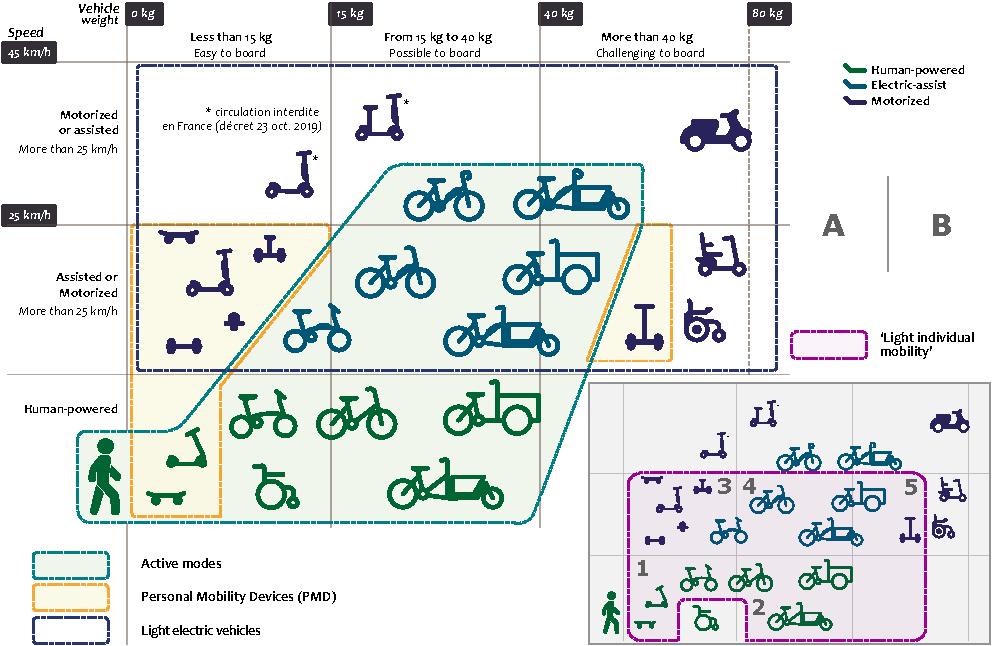
\includegraphics[width=1\columnwidth]{src/Figures/Chap-1/EN_Definition_perimetre_micromobilite.pdf}}
    \vspace{5pt}
    \begin{flushright}\scriptsize{
    Source (A): \textcolor{blue}{\textcite[61]{rabaud_quand_2022}}\index{Rabaud, Mathieu|pagebf}\index{Richer, Cyprien|pagebf}
    \\
    Graphic adaptation (B): \textcolor{blue}{Dylan Moinse (2023)}
    }\end{flushright}
\end{figure}

% Définition MIL
In this context, we propose to adopt an expression that we believe is more suitable for defining the scope of these diverse vehicles, while avoiding confusion related to the inclusion of walking or heavy vehicles. This reflection is based on the work of the ANR project \acrfull{URFé}\footnote{~
    The project, lasting 42 months, is organized into three components whose intersection allows for verifying the hypothesis of a gap between actual mobility practices and spatial planning logic: (i) the uses, effective practices, and safety issues, (ii) the built environment and its potential for accommodating low environmental impact mobility, and (iii) spatial planning as a public action through the lens of low environmental impact mobility \textcolor{blue}{\autocite{urfe_projet_2022}}.
}, under the scientific responsibility of \textcolor{blue}{Frédérique Hernandez}. This research project examines the hospitality of urban space towards new forms of low environmental impact mobility, using the urban areas of Lyon, Lausanne, Marseille–Aix-en-Provence, and Strasbourg as study areas \textcolor{blue}{\autocite{urfe_projet_2022}}\index{URFé@\textsl{URFé}|pagebf}. Although the expression \Commas{low environmental impact individual mobility modes,} used in this project, also has its limitations, in our view, regarding the precise delineation of the vehicles involved, we have chosen to adopt another concept from this research: that of \Commas{light individual mobility.} This expression was emphasized during the fourth collective seminar of the \acrshort{URFé} project, held on November 9, 2022, at \acrshort{Cerema} Hauts-de-France, and it seems particularly relevant for grouping the objects under study. Drawing inspiration from the framework proposed by \textcolor{blue}{\textcite[61]{rabaud_quand_2022}}\index{Rabaud, Mathieu|pagebf}\index{Richer, Cyprien|pagebf} in their chapter titled \Commas{When Personal Transport Devices Transform Urban Mobility,} and in relation to \hyperref[fig-chap1:perimetre-micromobilite]{Figure~\ref{fig-chap1:perimetre-micromobilite}} (page~\pageref{fig-chap1:perimetre-micromobilite}), we propose a definition perimeter for \Commas{light individual mobility} that goes beyond the frameworks of \Commas{active modes,} \acrshort{PMD}, \Commas{light electric vehicles,} and \Commas{intermediate vehicles.} This perimeter aims to include vehicles related to bicycles, micromobility, and their many variants. Our definition is based on partial inclusion of the \gls{active modes}, excluding walking, as well as \acrshort{PMD}, which exclude vehicles specifically designed for people with reduced mobility and some intermediate vehicles whose speeds exceed the regulatory limits for personal transport devices. Thus, \Commas{light individual mobility} encompasses a non-exhaustive list of popular vehicles (see \hyperref[fig-chap1:perimetre-micromobilite]{Figure~\ref{fig-chap1:perimetre-micromobilite}}, page~\pageref{fig-chap1:perimetre-micromobilite}):
    \begin{customitemize}
\item Muscular energy vehicles weighing less than 15 kilograms (cell 1), such as the skateboard, mechanical scooter, or folding bicycle;
\item Muscular energy vehicles weighing between 15 and 40 kilograms (cell 2), such as the classic bicycle, cargo bike (or biporteur), or tricycle;
\item Electric vehicles weighing less than 15 kilograms, with a maximum speed of 25 km/h (cell 3), such as the hoverboard, monowheel, \acrshort{PeS}, or electric unicycle;
\item Electric assist vehicles weighing between 15 and 40 kilograms, with a maximum speed of 25 km/h (cell 4), such as the folding electric bicycle, \acrshort{e-Bike}, electric cargo bike (or electric biporteur), or electric tricycle;
\item Electric vehicles weighing more than 40 kilograms, with a maximum speed of 25 km/h (cell 5), such as the segway;
\item Shared bikes and micromobility services, short or long-term rentals, with or without docking stations (cells 1 to 5), such as folding bikes in free service, \acrshort{PBS}, \acrshort{DESS}, \acrshort{e-Bike} in dockless sharing or service, electric cargo bikes in free service, or the segway for rent.
    \end{customitemize}%%Translated%%

% Transition
Within this family of \Commas{light individual mobility,} we maintain the subcategories associated with bicycles and their various derivatives, such as the folding bicycle, \acrshort{e-Bike}, or cargo bike, as well as \Commas{micromobility,} which primarily refers to the family of \acrshort{PMD}. These vehicles share a number of common characteristics: they are individual modes of transport, although some \Commas{intermediate modes} can accommodate an additional passenger. Their speed is limited, which allows for a form of proximity and interaction with the urban environment, fitting within the spirit of a \textsl{slow city} \textcolor{blue}{\autocite[103-108]{bu_tout-voiture_2024}}\index{Bu, Ludovic|pagebf}. Furthermore, these modes of transport are characterized by their low cost and their more inclusive nature, as they do not require a driving license, making them accessible to a wide range of users. They rely on a common system, conceptualized under the name \Commas{velomobility,} structured around a triptych based on territories, individuals, and uses \textcolor{blue}{\autocites[20-21]{rerat_au_2019}[492]{watson_how_2012}}\index{Rérat, Patrick|pagebf}\index{Watson, Matt|pagebf}. These vehicles, by nature, have potential for intermodality: they are either easily transportable in public transport or easily adapted for parking near a public transport hub. It is due to these various qualities that we will now focus more closely on the synergies between our two main objects of study: public transport and light individual mobility, drawing on the theoretical and strategic framework of \acrshort{TOD}. This approach will allow us to examine how \acrshort{TOD} can appropriate not only bicycles, as briefly explored in the context of \Commas{Hybrid Transit Metropolises} such as Copenhagen, but also the implications arising from the recent diversification of light individual mobility offerings. Through this analysis, we aim to highlight the synergetic links between these two systems.%%Translated%%

% 1.3.
\newpage
\needspace{1\baselineskip} % Reserve space
\sectionheader{Towards a \textsl{Micromobility-friendly Transit-Oriented Development}}
\section{New Perspectives for a \textsl{Transit-Oriented Development} Supported by the Integration of Light Individual Mobility
    \label{chap1:btod}
    }

    % Introduction
The improvement of scientific knowledge related to the development of public transport infrastructures has shown that they are not, by themselves, sufficient to form a viable alternative to \Commas{car dependency}\footnote{~
    \Commas{Car dependency} refers to the practice of traveling by car alone. It is derived from the term \Commas{autosolisme}. A political dictionary defines this term as \Commas{the act of traveling alone in a car, thus congesting the collective space, polluting, making noise, stressing for the benefit of a single person: the driver!} \textcolor{blue}{\autocite{carfreeEN_dictionnaire_2008}}\index{Carfree.fr@\textsl{Carfree.fr}|pagebf}. Occasionally, the antonym \Commas{carpooling} might be used, but it is more common to refer to \Commas{carpooling.}
}, across all areas \textcolor{blue}{\autocite[8]{molino_pratiques_2015}}\index{Molino, Marie|pagebf}\index{Rampon, Anne-Sophie|pagebf}\index{Cipolla, Romain|pagebf}. The traditional development of public transport supply requires simultaneous action on demand. Indeed, to effectively reduce car traffic, several strategies can be considered. One option is to reduce the urbanized area, which is difficult to achieve and accept. Another is to increase public transport coverage, which, however, could undermine the network's performance due to the high number of stops, thus compromising its competitiveness against the car. A more realistic option is to improve station accessibility \textcolor{blue}{\autocite[10]{verbavatz_critical_2019}}\index{Verbavatz, Vincent|pagebf}\index{Barthelemy, Marc|pagebf}. Research shows that the determining factor for the modal shift from car to public transport is accessibility to stations, rather than the qualitative improvement of the service \textcolor{blue}{\autocite[146]{brons_access_2009}}\index{Brons, Martijn|pagebf}\index{Givoni, Moshe|pagebf}\index{Rietveld, Piet|pagebf}. This observation aligns with the founding principle that mobility within transit-oriented neighborhoods, and especially prioritizing walking and cycling combined, constitutes a central lever for the success of a \acrshort{TOD} intervention. However, these modes of transport, while essential to public transport-oriented urban planning, are often overlooked or treated trivially, even though they play a decisive role in the success or failure of a \acrshort{TOD} project \textcolor{blue}{\autocite[34]{schlossberg_comparing_2004}}\index{Schlossberg, Marc|pagebf}\index{Brown, Nathaniel|pagebf}. Due to suburban sprawl, the performance and attractiveness of public transport networks have considerably diminished, due to longer distances and the dispersion of employment centers \textcolor{blue}{\autocite[13]{bentayou_transit-oriented_2015}}\index{Bentayou, Gilles|pagebf}. In this context, the intermodal approach incorporating cycling appears to be the most appropriate solution to address the challenges of the \Commas{first and last miles.} Cycling and public transport must thus maintain a symbiotic relationship: beyond just a feeder mode, cycling must be fully integrated into the travel experience, due to the strong competitiveness of this modal combination against the private car \textcolor{blue}{\autocite[208]{kager_characterisation_2016}}\index{Kager, Roland|pagebf}\index{Bertolini, Luca|pagebf}\index{te Brömmelstroet, Marco|pagebf}. Beyond cycling itself, it is now worth evaluating whether the \Commas{new mobility} modes that revolve around it can strengthen this dynamic. These emerging modes could indeed fit into a \Commas{bundle of modes and services} designed to maximize the benefits of a more resource-efficient alternative mobility system \textcolor{blue}{\autocite[134]{litman_new_2021}}\index{Litman, Todd|pagebf}.%%Translated%%

% Announcement of the plan
First, we will explore the arbitrary rule of walkable perimeter areas around \acrshort{TOD}\textcolor{blue}{s} and, more broadly, the need to expand transit-oriented neighborhoods through an intermodal approach. We will see that studies show how combined walking can extend far beyond the geographical perimeter usually attributed to it, while emphasizing that its reach, although relevant, remains insufficient to ensure optimal access to transport hubs in a suburbanization context. It thus appears essential to integrate other modes of transport that allow reaching more distant destinations, in order to enhance modal complementarity and optimize accessibility to hubs (\hyperref[chap1:btod-limites-tod]{section on a reinterpretation of combined walking, page~\pageref{chap1:btod-limites-tod}}). In this perspective, we will examine the comparative advantages of light individual mobility, which appears as a particularly suitable alternative to limit excessive reliance on cars. This reflection will lead us to discuss the recent development of a \acrfull{B-TOD}, or transit-oriented development integrating cycling, which highlights the potential of bicycles in extending the influence areas of public transport stations. Finally, in light of the modal diversity discussed earlier in this chapter, we will question the value of a more inclusive conceptualization integrating light individual mobility, through an \acrfull{M-TOD} (\hyperref[chap1:btod-definition]{section on a modal combination leveraging speed and \Commas{door-to-door} accessibility, page~\pageref{chap1:btod-definition}}).%%Translated%%

% 1.3.1.
\needspace{1\baselineskip} % Reserve space
\subsection{\Commas{Bursting the Bubble} of Pedestrian Pockets
    \label{chap1:btod-limites-tod}
    }

    % Introduction
The concept of \Commas{pedestrian pocket}, which predates \acrshort{TOD}, is based on the demarcation of an area within which walking is the preferred mode of transport, and where the main daily activities are concentrated \textcolor{blue}{\autocite[3]{kelbaugh_pedestrian_1989}}\index{Kelbaugh, Doug|pagebf}. Although widely integrated into the concept of urban planning, the pedestrian influence area of stations is often defined by arbitrary boundaries that do not necessarily reflect the actual practices of travelers, potentially resulting in a mismatch between the station neighborhood perimeter and the actual travel paths of users. From this observation, we align with recent scientific literature calling for a reconsideration of the real reach of combined walking. Indeed, pedestrian pathways to and from a station do not stop at the immediate scale of the station, but also influence the spatiotemporal distance users are willing to travel \textcolor{blue}{\autocite[52]{el_hadeuf_ville_2017}}\index{El Hadeuf, Mounya|pagebf}\index{Laterrasse, Jean|pagebf}. In this perspective, we propose to use this \Commas{bursting of the bubble} \textcolor{blue}{\autocite[33]{guerra_half-mile_2012}}\index{Guerra, Erick|pagebf} as an opportunity to redefine spatial planning by adopting a systemic or integrative approach \textcolor{blue}{\autocite[56]{kaufmann_retour_2014}}\index{Kaufmann, Vincent|pagebf} to highlight the advantages of intermodal travel. Such an approach would allow the development of spaces truly oriented towards public transport, defined on a more relevant spatial scale and likely to optimize modal shift towards the public transport network.%%Translated%%

% 1.3.1.1.
\needspace{1\baselineskip} % Reserve space
\subsubsection*{Questioning the \textsl{Doxa} of Confined \Commas{Pedestrian Pockets}
    \label{chap1:btod-limites-tod-marche-restreinte}
    }

    % Doxa
In France, as we have observed, we often witness the implementation of principles close to \Commas{\acrshort{TOD} without saying so} \textcolor{blue}{\autocite[273]{lo_feudo_scenario_2014}}\index{Lo Feudo, Fausto|pagebf}\index{Menerault, Philippe|pagebf}\index{L'Hostis, Alain|pagebf}\index{Festa, Demetrio Carmine|pagebf}. This multiplicity of interventions in the territory, related to this concept of urban planning, is often limited to punctual actions such as architectural renewal of stations or the redevelopment of adjacent spaces, giving less attention to larger scales, particularly the station neighborhood and its integration into the metropolitan area \textcolor{blue}{\autocite[50]{bentayou_transit-oriented_2015}}\index{Bentayou, Gilles|pagebf}. When \acrshort{TOD}\textcolor{blue}{s} specifically target the pedestrian influence areas of public transport nodes, they rely on a commonly accepted reference: that of 500 meters or 800 meters, the latter equating to 10 minutes of walking \textcolor{blue}{\autocite[1]{lhostis_perimetres_2016}}\index{L'Hostis, Alain|pagebf}, often defined as a \Commas{\textsl{Pedestrian Pocket}}. \textcolor{blue}{Peter} \textcolor{blue}{\textcite[56]{calthorpe_next_1993}}\index{Calthorpe, Peter|pagebf} recommends communities designed within 600 meters (approximately 2,000 feet) of a stop. \textcolor{blue}{\textcite[12]{bertolini_cities_2015}}\index{Bertolini, Luca|pagebf}\index{Spit, Tejo|pagebf}, in their book \foreignlanguage{english}{\textsl{Cities on Rails: The Redevelopment of Railway Stations and their Surroundings}} confirm that a 10-minute walking radius is an acceptable time-distance for accessing a station. A literature review on action perimeters around stations, conducted by \textcolor{blue}{\textcite[102]{guerra_half-mile_2012}}\index{Guerra, Erick|pagebf}\index{Cervero, Robert|pagebf}\index{Tischler, Daniel|pagebf}, shows, however, that this norm of 400 to 800 meters is frequently used without necessarily being backed by technical justifications. Yet, as we have seen in the evolution of \acrshort{TOD} thinking, one of the \Commas{5Ds} associated with this concept, distance to stations (\textsl{Distance to Transit}), is a central equation for measuring accessibility to public transport \textcolor{blue}{\autocite[267]{ewing_travel_2010}}\index{Ewing, Reid|pagebf}\index{Cervero, Robert|pagebf}. Over the past decade, research has sought to question this international standard of \Commas{800 meters} (\textsl{half-mile distance}), which has become a standard in \acrshort{TOD}\textcolor{blue}{s} \textcolor{blue}{\autocite[102]{guerra_half-mile_2012}}\index{Guerra, Erick|pagebf}\index{Cervero, Robert|pagebf}\index{Tischler, Daniel|pagebf}. The goal is to \Commas{burst the pedestrian bubble} \textcolor{blue}{\autocite[33]{guerra_half-mile_2012}}\index{Guerra, Erick|pagebf}, meaning to exceed the limits of the combined walking radius. This opens the way to a reinterpreted \acrshort{TOD} model, going beyond the spatial metaphor of the \Commas{bull’s eye} \textsl{(the bull’s eye concept)} \textcolor{blue}{\autocite[28]{curtis_transit_2009}}\index{Curtis, Carey|pagebf}\index{Renne, John Luciano|pagebf}\index{Bertolini, Luca|pagebf}.%%Translated%%

% Urban planning documents
This commonly accepted rule, based on the 800-meter pedestrian perimeter, is frequently applied and visible in the urban planning guidelines. Urban planners typically use this limit as the action perimeter around stations \textcolor{blue}{\autocite[40]{olszewski_using_2005}}\index{Olszewski, Piotr~S.|pagebf}\index{Wibowo, Sony Sulaksono|pagebf}. Already in the \textsl{Regional Transport Scheme} of the former \textcolor{blue}{\textcite[21]{region_nord-pas-de-calais_schema_2006}}\index{Région Nord-Pas-de-Calais@\textsl{Région Nord-Pas-de-Calais}|pagebf}, walking was identified as a mode to prioritize for short-distance feeder trips to bus or coach stops, train stations, and interchange hubs. The \acrfull{PDU} 2010-2020 of the \acrfull{MEL} incorporated this approach by defining \acrfull{DIVAT}, corresponding to strategic areas located around metropolitan stations, subway and tramway stations, as well as \acrfull{BRT} stops. These strategic perimeters were then shaped into a 500-meter radius circle \textcolor{blue}{\autocite[39]{lmcu_plan_2011}}\index{LMCU@\textsl{LMCU}|pagebf}. In line with this \acrshort{PDU}, the \acrshort{DIVAT} were faithfully incorporated into the \acrfull{PLH} 2012-2018 of the \acrshort{MEL}, with an extension to bus stops recording more than sixty daily passages in all directions \textcolor{blue}{\autocite[4]{lmcu_2e_2012}}\index{LMCU@\textsl{LMCU}|pagebf}. These principles were then integrated into the 2020 \acrfull{PLUi} of the \acrfull{EPCI}, thereby enhancing the consistency between the various territorial planning tools \textcolor{blue}{\autocite[44]{metropole_europeenne_de_lille_plan_2019-3}}\index{LMCU@\textsl{LMCU}|pagebf}. However, some strategic studies have revisited these station perimeters to adapt them to varied contexts. For example, the Grand Paris Express station observatory initially defined an 800-meter bird's-eye view perimeter for the 69 stations under construction \textcolor{blue}{\autocite[1]{apur_observatoire_2017}}\index{Apur@\textsl{Apur}|pagebf}. This framework was later evolved to propose two additional levels: 500 meters for stations in the city center and 1,000 meters for \acrfull{RER} stations and those of the Grand Paris Express \textcolor{blue}{\autocite[13]{apur_observatoire_2018}}\index{Apur@\textsl{Apur}|pagebf}. Finally, particular attention was given to a 2,000-meter radius for the cycling scale \textcolor{blue}{\autocite[22]{apur_observatoire_2018}}\index{Apur@\textsl{Apur}|pagebf}.%%Translated%%

% Expansion of primary areas
Some consider that combined walking can reach spatio-temporal distances well beyond those dictated by the Anglo-Saxon rule of 400 or 800 meters, or even 10 minutes, within the perimeter of the \Commas{primary area} as imagined by \textcolor{blue}{Peter} \textcolor{blue}{\textcite[56]{calthorpe_next_1993}}\index{Calthorpe, Peter|pagebf}. In a literature review, the researcher in geography, specializing in planning and mobility, \textcolor{blue}{Alain} \textcolor{blue}{\textcite[5]{lhostis_perimetres_2016}}\index{L'Hostis, Alain|pagebf} highlights that some European train stations or metro stations record walking distances easily reaching one to two kilometers. The practice of combined walking (\textsl{walk-and-ride}) around well-served transport hubs, benefiting from high frequencies, extensive coverage, and good accessibility, is thus marked by an extension of its socially accepted distances. These neighborhoods, which are both dense, mixed, and feature high-quality public space design, particularly in terms of \gls{walkability}, embody the principles of \acrshort{TOD} neighborhoods \textcolor{blue}{\autocites[79]{ker_myths_2003}[7]{lhostis_perimetres_2016}[30]{hasiak_access_2019}}\index{Hasiak, Sophie|pagebf}\index{L'Hostis, Alain|pagebf}\index{Ker, Ian|pagebf}\index{Ginn, Simon|pagebf}. Research shows that in this context, walking trips far exceed the traditionally accepted 800-meter threshold \textcolor{blue}{\autocites[79]{ker_myths_2003}[7]{lhostis_perimetres_2016}[30]{hasiak_access_2019}}\index{Hasiak, Sophie|pagebf}\index{L'Hostis, Alain|pagebf}\index{Ker, Ian|pagebf}\index{Ginn, Simon|pagebf}.%%Translated%%

% Pedestrian Corridor
\begin{carte}[h!]\vspace*{4pt}
    \caption{Extension of the station area through the enhancement of a densified and walkable corridor.}
    \label{fig-chap1:tod-corridor-pieton}
    \centerline{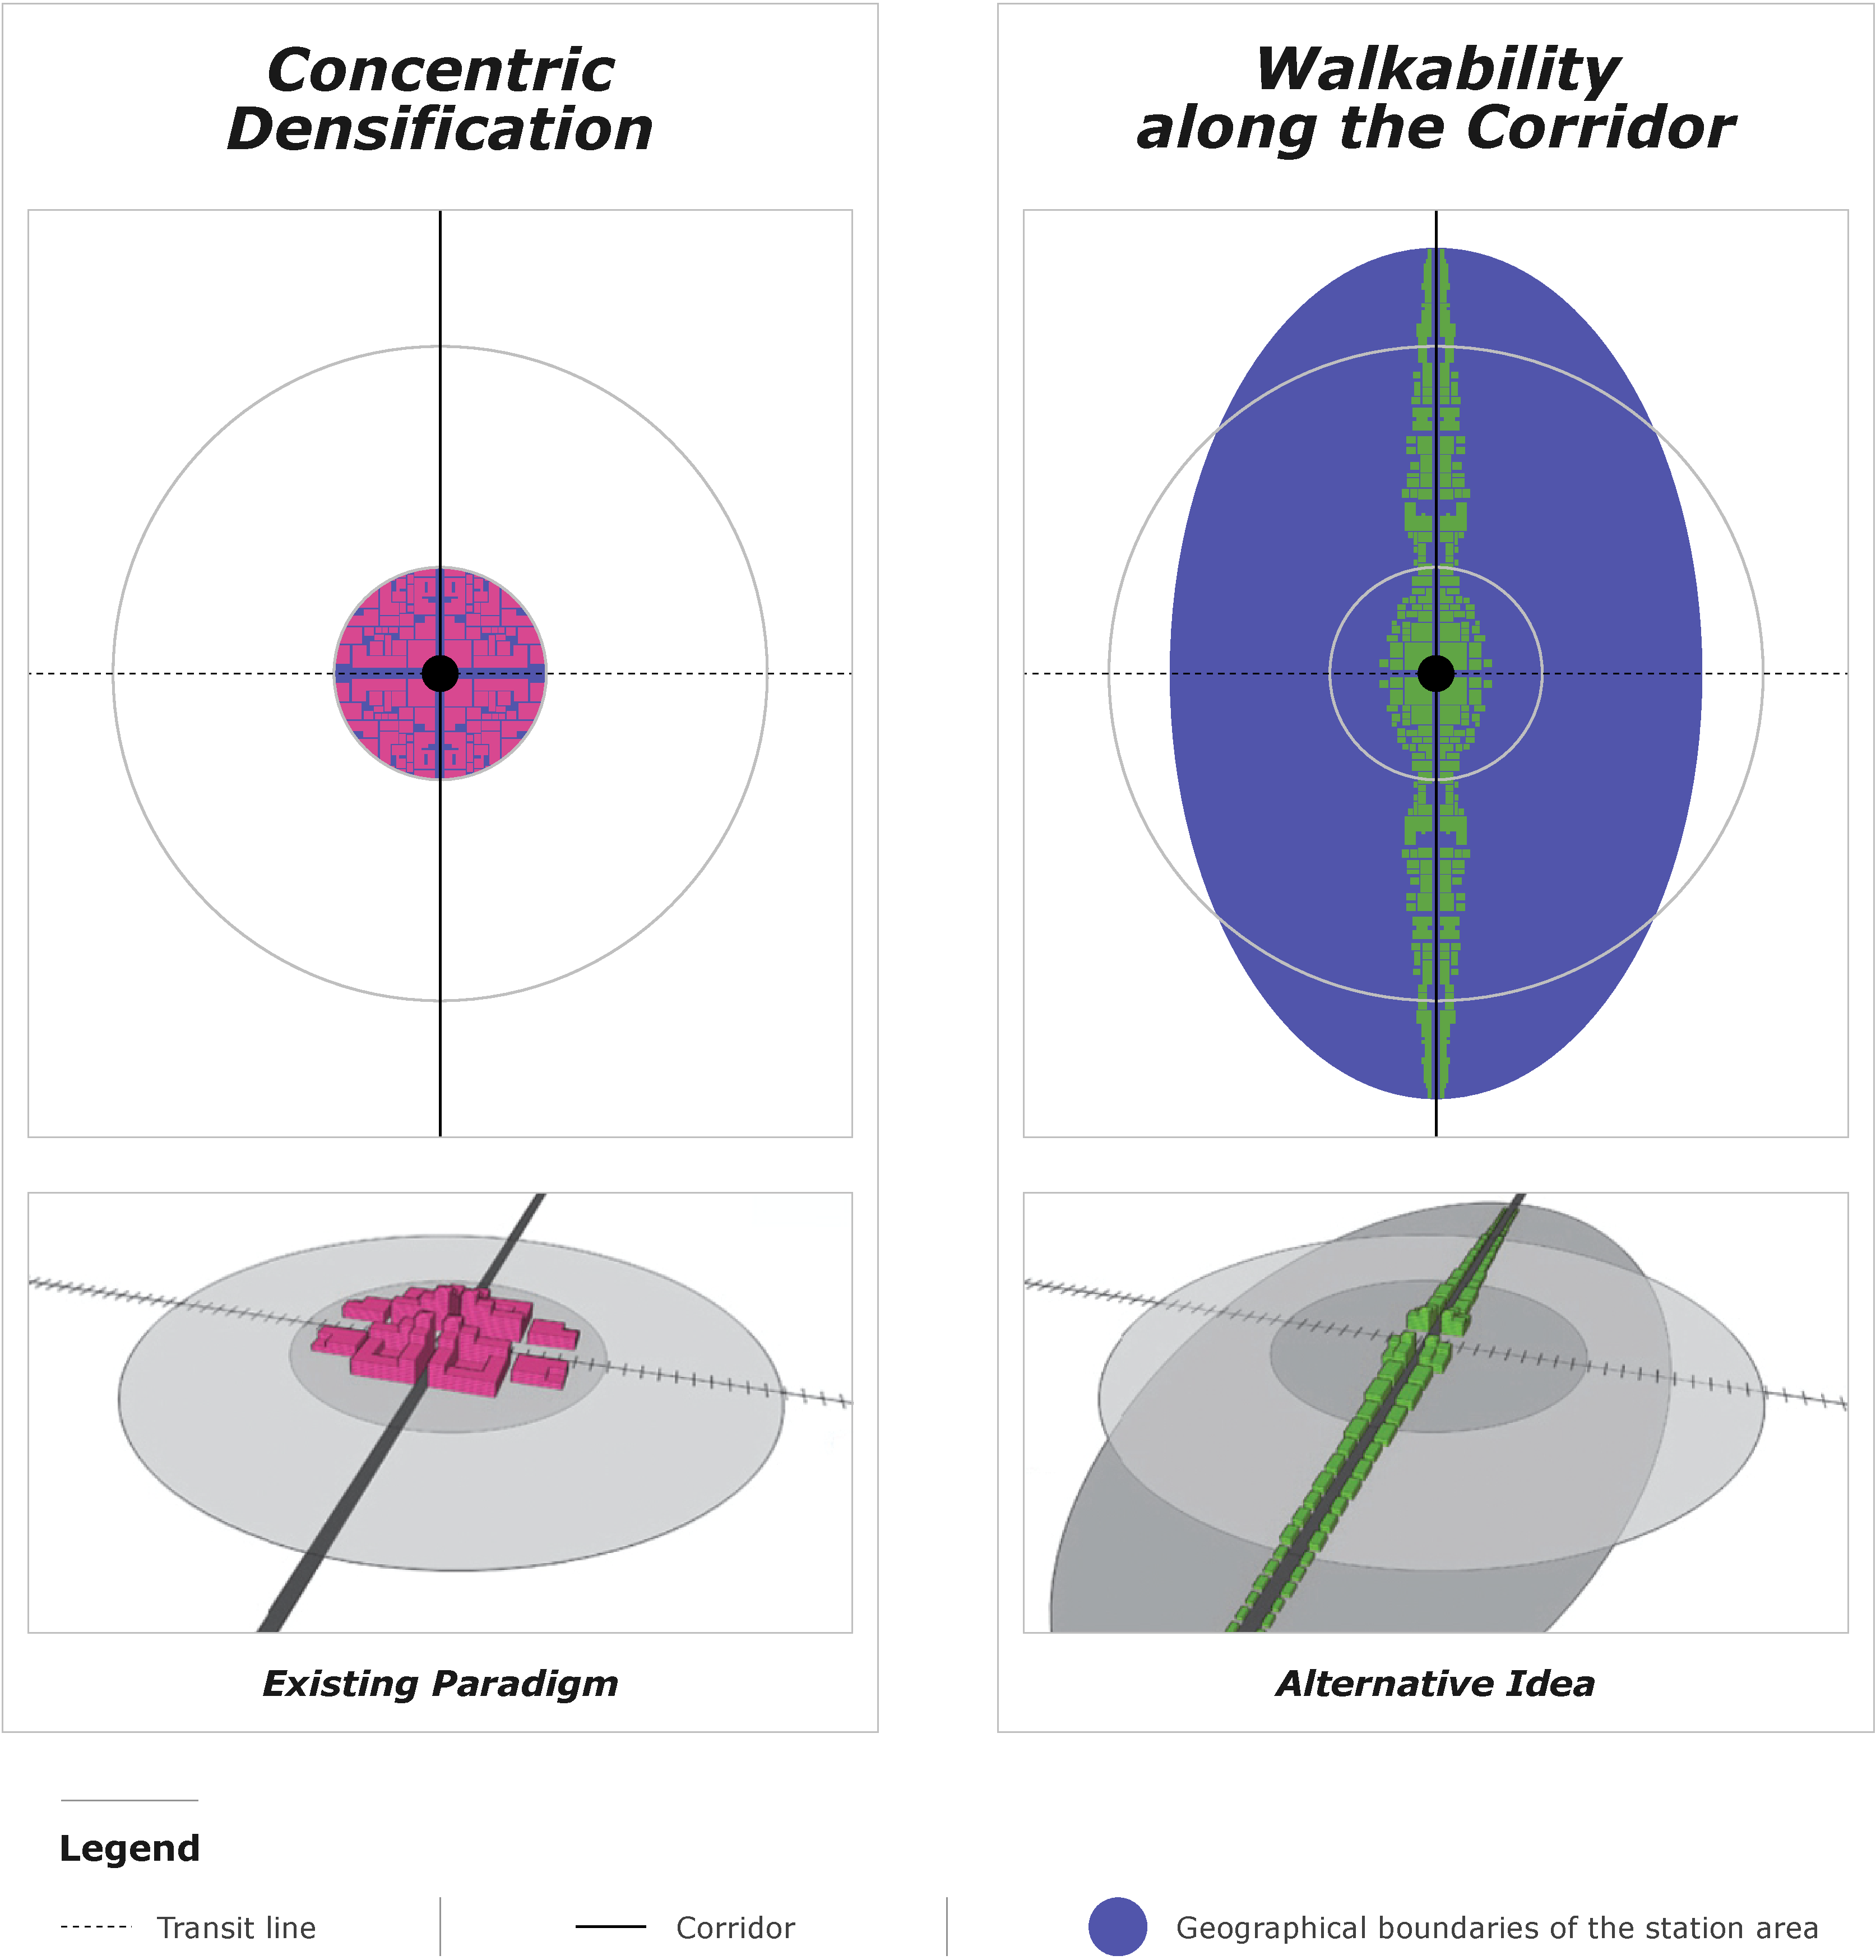
\includegraphics[width=1\columnwidth]{src/Figures/Chap-1/EN_Corridor_pieton.pdf}}
    \vspace{5pt}
    \begin{flushright}\scriptsize{
    Source: \textcolor{blue}{\textcite[163]{park_can_2015}}\index{Park, Sungjin|pagebf}\index{Deakin, Elizabeth|pagebf}\index{Jang, Kitae|pagebf}
    \\
    Graphic adaptation: \textcolor{blue}{Dylan Moinse (2025)}
    }\end{flushright}
\end{carte}

% Examples
Many studies today focus on the distance traveled by travelers to walk to or from a public transport station, generally supporting an underestimation of the pedestrian perimeters traditionally accepted around these nodes. On average, pedestrians accessing a train or metro station walk 1 kilometer, whether in San Francisco \textcolor{blue}{\autocite[5]{cervero_walk-and-ride_2001}}\index{Cervero, Robert|pagebf} or Singapore \textcolor{blue}{\autocite[41]{olszewski_using_2005}}\index{Olszewski, Piotr~S.|pagebf}\index{Wibowo, Sony Sulaksono|pagebf}. Using the 85\textsuperscript{th} percentile of the cumulative distance distribution, studies have shown that a distance of 1 kilometer (about 12 minutes walking) is considered acceptable around metro stations in Beijing \textcolor{blue}{\autocite[720]{yang_study_2013}}\index{Yang, Rongrong|pagebf}\index{Yan, Hai|pagebf}\index{Xiong, Wen|pagebf}\index{Liu, Tao|pagebf}, while slightly longer distances, 1.2 (for access) and 1.1 kilometers (for egress), are observed around train stations in Montreal \textcolor{blue}{\autocite[9]{el-geneidy_pedestrian_2009}}\index{El-Geneidy, Ahmed~M.|pagebf}\index{Tétreault, Paul|pagebf}\index{Surprenant-Legault, Julien|pagebf}. In the southeast of England, distances even reach 1.6 kilometers around stations \textcolor{blue}{\autocite[14]{bunn_how_2015}}\index{Bunn, Nick|pagebf}\index{Wakenshaw, Gareth|pagebf}. In the case of the Nord-Pas-de-Calais region, the 90\textsuperscript{th} percentile of rail passengers reveals that distances can reach 20 minutes on foot, compared to an observed average of 11 minutes \textcolor{blue}{\autocite[17]{hasiak_estimation_2018}}\index{Hasiak, Fabrice|pagebf}\index{Lannoy, Arnaud|pagebf}\index{Bodard, Géraldine|pagebf}\index{Palmier, Patrick|pagebf}. These variations reflect the major influence of certain urban environmental parameters, which can expand or contract these perceived distances \textcolor{blue}{\autocite[17]{soest_exploring_2020}}\index{Soest, Dennis van|pagebf}\index{Tight, Miles~R.|pagebf}\index{Rogers, Christopher~D.~F.|pagebf}. Already in 1984, \textcolor{blue}{Richard~k.} \textcolor{blue}{\textcite[23-59]{untermann_accommodating_1984}}\index{Untermann, Richard~K.|pagebf}, in his book \foreignlanguage{english}{\textsl{Accommodating the Pedestrian: Adapting Towns and Neighborhoods for Walking and Biking}}, showed that the maximum walking range in suburban areas, often confined to rigid thresholds of 400, 500, or 800 meters, could be considerably extended—even doubled—by designing attractive urban spaces and pleasant pedestrian corridors. More recent research confirms that urban diversity plays a key role. For example, a comparative study between Beijing, Tianjin, and Shenzhen indicates that pedestrians often double their walking distances when the urban environment features a high level of mixed-use, with shops and offices near transport stations \textcolor{blue}{\autocite[12]{zacharias_local_2017}}\index{Zacharias, John|pagebf}\index{Zhao, Qi|pagebf}. Similarly, in Australia and the United States, travelers are willing to walk an additional 800 meters when the urban environment follows the principles of \acrshort{TOD} \textcolor{blue}{\autocite[33]{canepa_bursting_2007}}\index{Canepa, Brian|pagebf}. Improving \Commas{micro-walkability} elements, particularly by strategically designing pedestrian corridors, appears to be a key lever to extend these spatial perimeters. Thus, \textcolor{blue}{\textcite[163]{park_can_2015}}\index{Park, Sungjin|pagebf}\index{Deakin, Elizabeth|pagebf}\index{Jang, Kitae|pagebf} demonstrate that it is possible to encourage public transport users to walk much greater distances by improving pedestrian infrastructure (see \hyperref[fig-chap1:tod-corridor-pieton]{Map~\ref{fig-chap1:tod-corridor-pieton}}, page~\pageref{fig-chap1:tod-corridor-pieton}). For example, creating pedestrian streets around stations increases the acceptable walking range to stations by 20\% in the United States, and by up to 120\% in Germany \textcolor{blue}{\autocite[151]{zielstra_comparative_2011}}\index{Zielstra, Dennis|pagebf}\index{Hochmair, Hartwig~H.|pagebf}.%%Translated%%

% Conclusion + Transition
Whether it's a pedestrian access area, represented as an Euclidean extent (circle) or calculated based on the road network (isodistance or isochrone), the arbitrary rule of 800 meters or 10 minutes of walking is more of a historical artifact than an analytical and statistical construction \textcolor{blue}{\autocite[102]{guerra_half-mile_2012}}\index{Guerra, Erick|pagebf}\index{Cervero, Robert|pagebf}\index{Tischler, Daniel|pagebf}. This rule, while commonly used, demonstrates its limitations. Indeed, while the primary service area perimeter of public transport stations, estimated at 800 meters, is not fundamentally incorrect—average distances for intercity rail often reaching 1,000 meters—the real difference lies in the method of measurement. By adopting an approach based on \Commas{acceptable} distance (considering the 85\textsuperscript{th} or 90\textsuperscript{th} percentiles) rather than just observable distance, it becomes clear that traditional pedestrian perimeters underestimate the actual distances traveled and experienced by users. For example, one study shows that traditional thresholds of 400 and 800 meters underestimate by 30\% the actual coverage of public transport accessible by foot in the Montreal region \textcolor{blue}{\autocite[20]{el-geneidy_new_2014}}\index{El-Geneidy, Ahmed~M.|pagebf}\index{Grimsrud, Michael|pagebf}\index{Wasfi, Rania|pagebf}\index{Tétreault, Paul|pagebf}\index{Surprenant-Legault, Julien|pagebf}. This highlights the need to move beyond the classical conception of walking. In France, while the average duration of pedestrian trips is 13 minutes, it is important to differentiate between monomodal walking and combined walking, used as a mode of connection to public transport stations. Indeed, while four out of five pedestrian trips in France last less than 15 minutes, those associated with combined walking frequently reach 20 minutes around train stations \textcolor{blue}{\autocite[23]{solere_mobilite_2010}}\index{Solere, Régis de|pagebf}\index{Papon, Francis|pagebf}. This increased range of combined walking is increasingly recognized in academic research, which considers it extendable depending on factors that enhance the \acrshort{TOD} potential of territories, such as urban density, functional mix, or the quality of pedestrian infrastructure. However, in peripheral neighborhoods, where the distances required to access public transport are much greater, walking alone is insufficient to correct these imbalances \textcolor{blue}{\autocite[85]{cervero_bike-and-ride_2013}}\index{Cervero, Robert|pagebf}\index{Caldwell, Benjamin|pagebf}\index{Cuellar, Jesus|pagebf}. To overcome the dichotomy between walking and public transport in central areas, and the car in intermodal areas in the suburbs, cycling can be the missing link in the intermodal chain. Yet, while academic and technical literature focuses almost exclusively on the accessibility of stations by foot, bike accessibility remains largely marginalized and under-studied \textcolor{blue}{\autocite[283]{martens_bicycle_2004}}\index{Martens, Karel|pagebf}. This gap represents a challenge to fully integrate cycling into accessibility and intermodality strategies, especially in areas where distances exceed the traditional capacities of walking.%%Translated%%

% 1.3.1.2.
\needspace{1\baselineskip} % Réserve de l'espace
\subsubsection*{Correcting the Weaknesses of Public Transport through an Intermodal Approach
    \label{chap1:btod-definition-intermodalite}
    }

    % Limitations of Walking
Given the limitations related to the reach of walking, which sometimes makes access to public transport stations restrictive, the effectiveness of \acrshort{TOD} is now being questioned. Indeed, the urban growth of territories has largely been based on distances adapted to the scale of the car, resulting in urban sprawl, often seen as a form of \Commas{suburbanization}. Furthermore, while public transport is effective in some respects, it lacks the flexibility advantages associated with the automobile \textcolor{blue}{\autocite[209]{heran_retour_2015}}\index{Héran, Frédéric|pagebf}. This situation calls into question the ability of the urban model to effectively combat dependence on motorized modes. Public transport represents only a partially adapted solution to reduce excessive reliance on the car. An alternative lies in the promotion of intermodality, which could address the rigidity of the public transport network \textcolor{blue}{\autocite[17]{wiel_comment_1998}}\index{Wiel, Marc|pagebf} and improve the overall efficiency of the mobility system \textcolor{blue}{\autocite[82]{oostendorp_combining_2018}}\index{Oostendorp, Rebekka|pagebf}\index{Gebhardt, Laura|pagebf}. Indeed, intermodality helps extend the influence area of nodes by integrating complementary solutions \textcolor{blue}{\autocite[16]{amar_homo_2016}}\index{Amar, Georges|pagebf}, which could strengthen their relevance in urban and suburban contexts marked by car dependency.%%Translated%%

% Intermodality
Interconnection refers to the link between two or more transport networks that are heterogeneous in their technical, organizational, and institutional dimensions, often associated with distinct mobility scales \textcolor{blue}{\autocites[]{dupuy_reseaux_1988}{varlet_interconnexion_1992}}\index{Dupuy, Gabriel|pagebf}\index{Varlet, Jean|pagebf}. The interest in this transition between different mobility regimes lies in the ability to go beyond the simple juxtaposition of unimodal networks that were not designed to be coordinated. This approach helps better understand the \Commas{concept-interface}, which relates multiple speeds of movement and spatial scales \textcolor{blue}{\autocite[156]{peters_time_1960}}\index{Peters, Peter Frank|pagebf}. This intermodal integration results in the formation of a meta-network, defined as a network of actual networks. It is a multiscalar nesting of systems that, through their interconnection, create an integrated megasystem \textcolor{blue}{\autocite[89]{ageron_intermodalite-voyageurs_2013}}\index{Ageron, Pierre|pagebf}\index{Varlet, Jean|pagebf}. Intermodal passenger mobility thus becomes a system-object, as a geographically located actor organization that generates places and practices \textcolor{blue}{\autocite[15]{varlet_interconnexion_1992}}\index{Varlet, Jean|pagebf}. Largely linked to public transport, intermodal passenger mobility is recognized as the most resource-efficient option in terms of travel time, cost, or energy consumption for making a trip from point A to point B \textcolor{blue}{\autocite[73]{oostendorp_combining_2018}}\index{Oostendorp, Rebekka|pagebf}\index{Gebhardt, Laura|pagebf}. In this sense, scheduling, interconnection, and intermodality of networks constitute efficiency factors that align with the principle of \Commas{reliance}. This principle, as a creator of links and synergies between varied flows, underpins new forms of network optimization \textcolor{blue}{\autocite[16-17]{amar_homo_2016}}\index{Amar, Georges|pagebf}. This evolution is accompanied by a growing modal diversification, driven by processes of (re)invention, technical and service innovation, as well as modal hybridization phenomena. These dynamics go beyond the binary vision of simply shifting from car use to public transport, promoting a multimodal and intermodal approach \textcolor{blue}{\autocite{richer_dossier_2021}}\index{Richer, Cyprien|pagebf}.%%Translated%%

% Figure functions and components of intermodality
\begin{figure}[h!]\vspace*{4pt}
    \caption{Functions and components of the intermodal system.}
    \label{fig-chap1:composantes-fonctions-intermodalite}
    \centerline{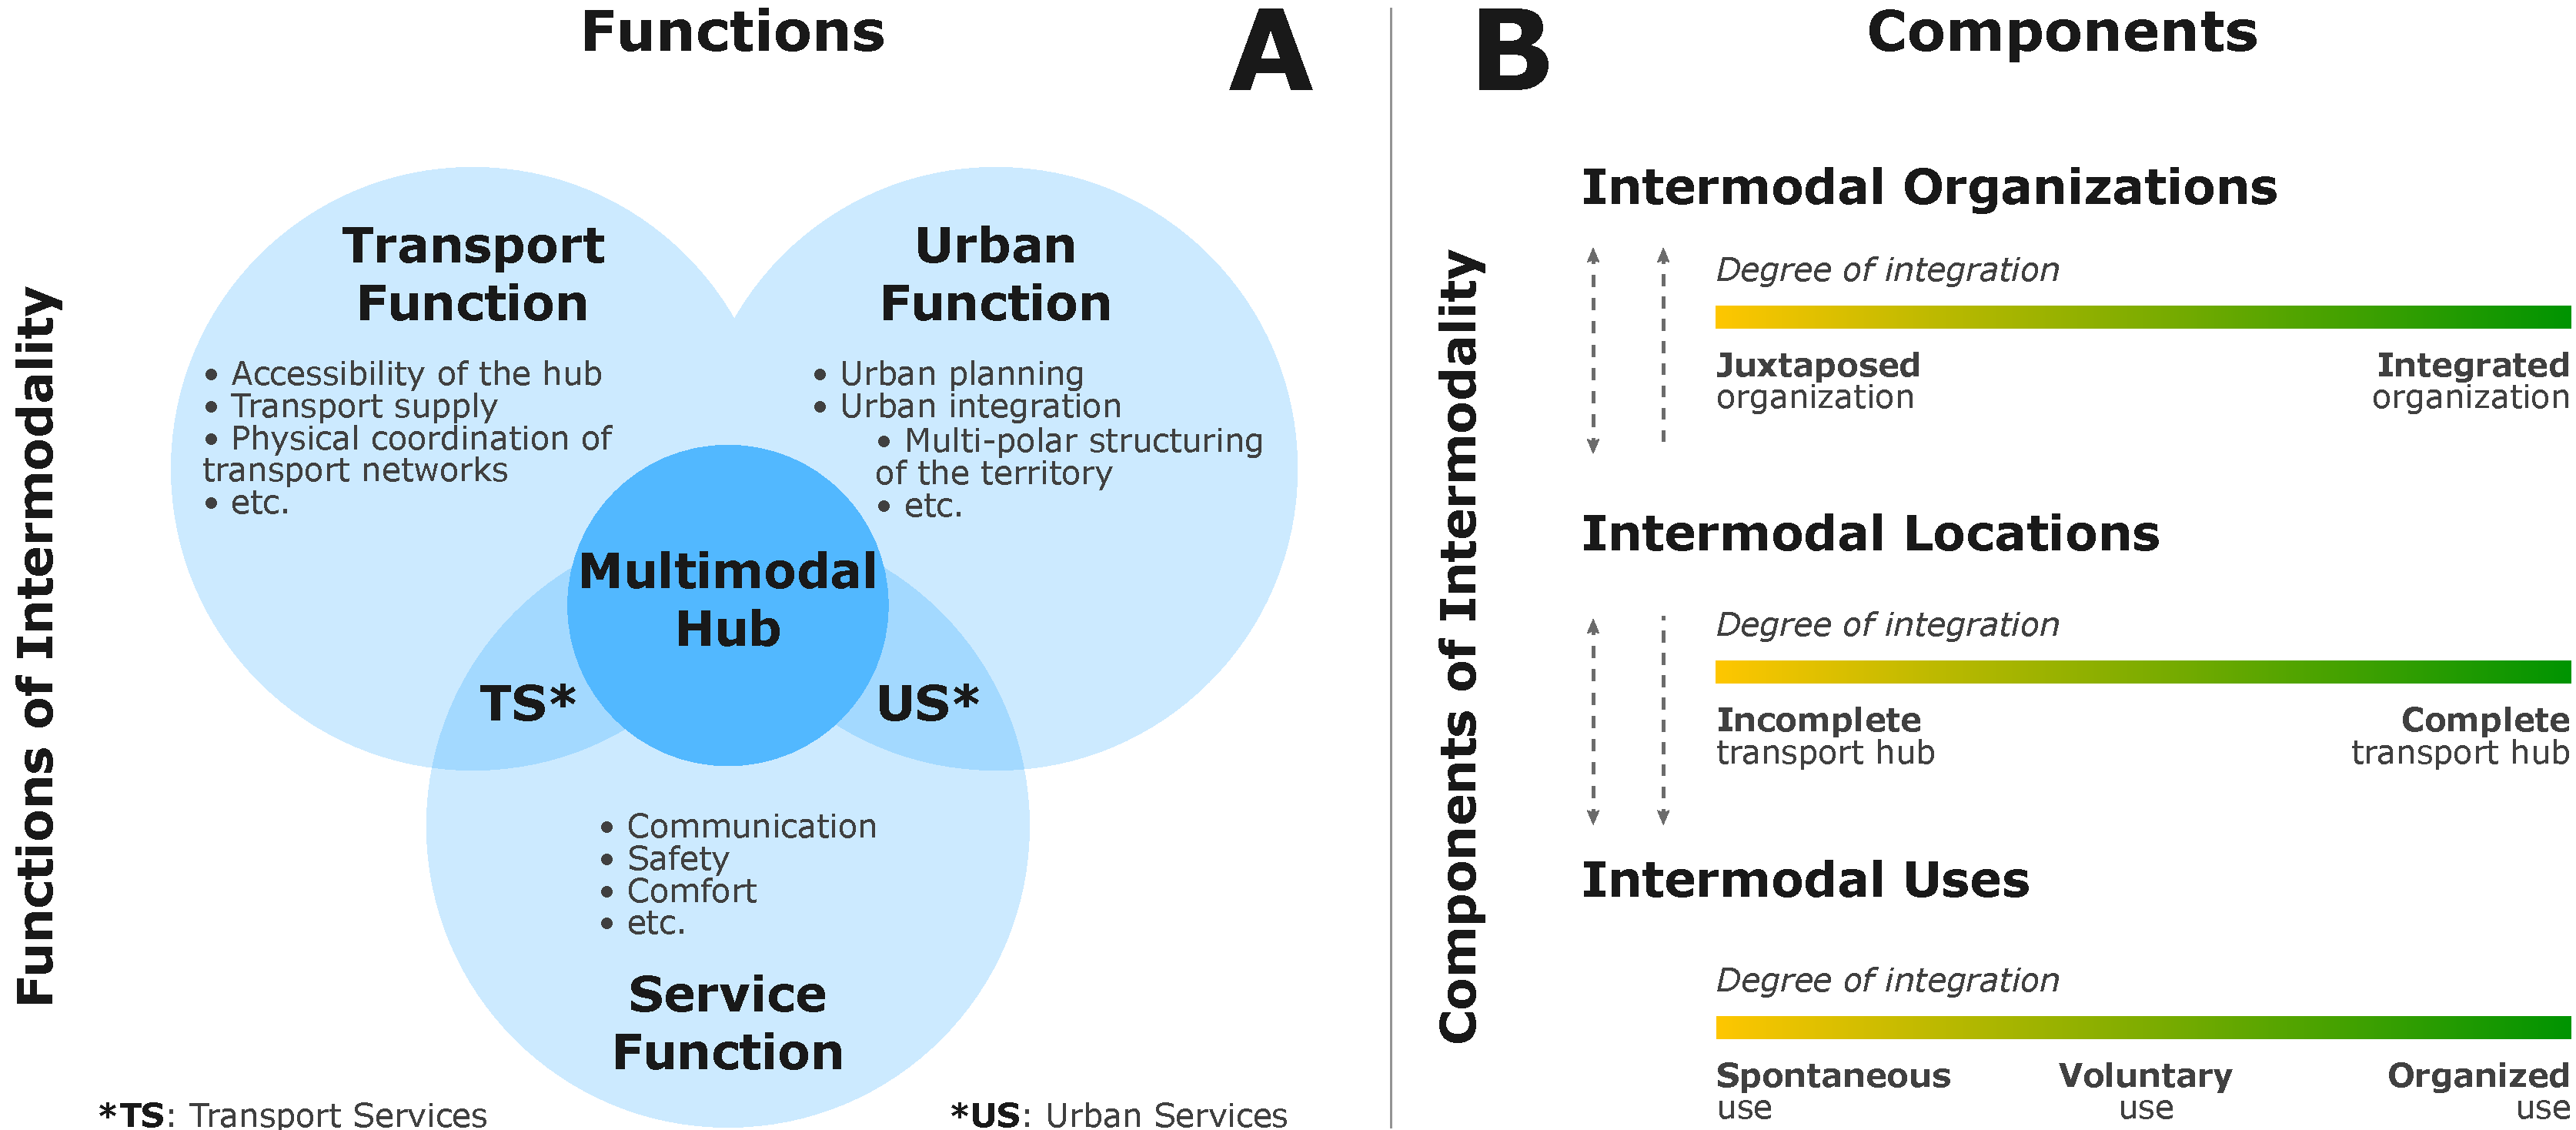
\includegraphics[width=1\columnwidth]{src/Figures/Chap-1/EN_Fonctions_Composants_Intermodalite.pdf}}
    \vspace{5pt}
    \begin{flushright}\scriptsize{
    Source (A): \textcolor{blue}{Cyprien} \textcolor{blue}{\textcite[14]{richer_lemergence_2008}}\index{Richer, Cyprien|pagebf}
    \\
    Source (B): \textcolor{blue}{Sandra} \textcolor{blue}{\textcite[167]{bozzani_grandes_2006}}\index{Bozzani-Franc, Sandra|pagebf}\index{Paris, Didier|pagebf}\index{Bakis, Henry|pagebf}\index{Menerault, Philippe|pagebf}
    \\
    Graphic adaptation: \textcolor{blue}{Dylan Moinse (2023)}
    }\end{flushright}
\end{figure}

% Intermodal System
The notion of intermodal passenger mobility can be analyzed through three main components proposed by \textcolor{blue}{Sandra} \textcolor{blue}{\textcite[167]{bozzani_grandes_2006}}\index{Bozzani-Franc, Sandra|pagebf}\index{Paris, Didier|pagebf}\index{Bakis, Henry|pagebf}\index{Menerault, Philippe|pagebf} in her doctoral thesis on the contribution of high-speed aero-rail intermodality (see \hyperref[fig-chap1:composantes-fonctions-intermodalite]{Figure~\ref{fig-chap1:composantes-fonctions-intermodalite}}, page~\pageref{fig-chap1:composantes-fonctions-intermodalite}). This tripartite framework is based on the \textsl{existence of an intermodal organization}, the \textsl{location in an intermodal space}, and \textsl{specific intermodal uses}, each dimension interacting with the others. These three aspects allow for evaluating the degree of integration of interconnection hubs based on the quality of service provided\footnote{~
    The quality of service in intermodality is expressed through cooperation and complementarity between operators, the coordination of schedules, the availability of intermodal information, the pooling of ticket reservations, a facilitated connection between modes, optimized connection and waiting times, and luggage handling \textcolor{blue}{\autocites[65]{bozzani_intermodalite_2005}[167]{bozzani_grandes_2006}}\index{Bozzani-Franc, Sandra|pagebf}\index{Paris, Didier|pagebf}\index{Bakis, Henry|pagebf}\index{Menerault, Philippe|pagebf}.
} \textcolor{blue}{\autocites[65]{bozzani_intermodalite_2005}[167]{bozzani_grandes_2006}}\index{Bozzani-Franc, Sandra|pagebf}\index{Paris, Didier|pagebf}\index{Bakis, Henry|pagebf}\index{Menerault, Philippe|pagebf}. Intermodality, made up of these three interrelated subsystems, requires an organization, is located in a space, and is made of uses. It thus allows for addressing key concepts in social sciences, such as the individual, place, and the world, as explained by \textcolor{blue}{Pierre} \textcolor{blue}{\textcite[490]{ageron_intermodalite-voyageurs_2013}}\index{Ageron, Pierre|pagebf}\index{Varlet, Jean|pagebf}. These subsystems are based on the principle of transcalarities, that is, an articulation between different spatial scales, a prerequisite for the complementarity of modes of transportation. Indeed, an intermodal association would not be of interest to the user if the modes involved were redundant in terms of territorial service and therefore of possible destinations \textcolor{blue}{\autocite[45]{ageron_intermodalite-voyageurs_2013}}\index{Ageron, Pierre|pagebf}\index{Varlet, Jean|pagebf}. From this perspective, intermodality is not limited to a simple succession of modes during a trip. It becomes a true \Commas{territorial resource}, understood as a combination of \Commas{production factors} that facilitate the proximity of spatial actors, in accordance with the definition by \textcolor{blue}{\textcite[6]{gumuchian_ressource_2007}}\index{Gumuchian, Hervé|pagebf}\index{Pecqueur, Bernard|pagebf}. In this regard, \textcolor{blue}{Cyprien} \textcolor{blue}{\textcite[14]{richer_lemergence_2008}}\index{Richer, Cyprien|pagebf}, then a research officer in geography at \acrshort{Cerema}, emphasizes the three constitutive functions of exchange hubs (see \hyperref[fig-chap1:composantes-fonctions-intermodalite]{Figure~\ref{fig-chap1:composantes-fonctions-intermodalite}}, page~\pageref{fig-chap1:tad-murdoch}): the \textsl{transport function}, the \textsl{urban function}, and the \textsl{service function}. These functions ensure not only the interconnection of networks but also the structuring of territories. The experiences with \textsl{Mobility Hubs}, conceptualized as part of the Interreg \textsl{Mobi-Mix} project, provide an illustration. They constitute points of intermodal facilitation, designed as physical hubs integrating at least two shared mobility systems, as evidenced in pilot projects in Norfolk and Valenciennes \textcolor{blue}{\autocites[3498]{hachette_exploring_2023}[248]{hachette_mobility_2023}}\index{Hachette, Maxime|pagebf}\index{L'Hostis, Alain|pagebf}\index{Gragera, Albert|pagebf}.%%Translated%%

% Relevance of MIL + Transition
According to \textcolor{blue}{\textcite[116]{goletz_intermodality_2020}}\index{Goletz, Mirko|pagebf}\index{Haustein, Sonja|pagebf}\index{Wolking, Christina|pagebf}\index{L'Hostis, Alain|pagebf}, strategic considerations on intermodality are increasingly prominent in the spatial planning directions. This trend reflects a promise of reducing car traffic, limiting car ownership, and acting as a catalyst for a genuine modal shift towards public transportation. Additionally, there is the idea that, in the future, new modes of transport that are still little used today will see an increase in their use and will significantly contribute to enriching intermodal chains. In this regard, \textcolor{blue}{\textcite[77]{oostendorp_combining_2018}}\index{Oostendorp, Rebekka|pagebf}\index{Gebhardt, Laura|pagebf} predict that the emergence of new forms of mobility, such as light individual mobility, will make intermodality even more relevant in the years to come. Integrating these \Commas{micro-modes} into public transport systems could provide many \Commas{co-benefits}, such as economic opportunities, health benefits, better inclusivity, cost savings for users, reductions in accidents and road congestion, as well as improvements in comfort and personal well-being \textcolor{blue}{\autocite[39-40]{litman_new_2021}}\index{Litman, Todd|pagebf}. In this context, light individual mobility positions itself as a family of modes complementary to public transport, similar to combined walking. It is likely to bring greater resilience to public transport systems \textcolor{blue}{\autocites{heran_velo_2020}[6]{dezobry_du_2020}}\index{Héran, Frédéric|pagebf}\index{Dezobry, Guillaume|pagebf}\index{Fontenelle, Louis de|pagebf}\index{Staropoli, Carine|pagebf}.%%Translated%%

% 1.3.2.
\needspace{1\baselineskip} % Reserve space
\subsection{From a \Commas{Station-to-Station} Approach to a \Commas{Door-to-Door} Approach
    \label{chap1:btod-definition}
    }

% Introduction
Categories of mobility that have long been considered antagonistic, such as individual transport and public transport, are gradually evolving towards a logic of \Commas{transmodality}. The emergence of intermodal configurations, made possible by the diversification of light individual mobility, thus promotes the affirmation of \Commas{individual public transport} \textcolor{blue}{\autocites[14-15]{amar_homo_2016}[18]{fijalkow_sociologie_2017}[5]{kostrzewska_towards_2017}}\index{Amar, Georges|pagebf}\index{Kostrzewska, Małgorzata|pagebf}\index{Macikowski, Bartosz|pagebf}\index{Fijalkow, Yankel|pagebf}. These compact vehicles provide an intelligent response to the challenges of the \Commas{first and last miles}, offering a \Commas{door-to-door} mobility solution that was long lacking in public transport \textcolor{blue}{\autocite{dia_banning_2019}}\index{Dia, Hussein|pagebf}. Integrated into an intermodal approach, light individual mobility is not limited to its technical specifics or its mode of acquisition: it generates unique travel practices that contribute to transforming mobility usage \textcolor{blue}{\autocite[1]{tuncer_notes_2020}}\index{Tuncer, Sylvaine|pagebf}\index{Laurier, Eric|pagebf}\index{Brown, Barry|pagebf}\index{Licoppe, Christian|pagebf}. Its potential lies notably in its ability to address the service gaps in public transport \textcolor{blue}{\autocites{gauquelin_case_2021}[3]{lee_forecasting_2021}}\index{Gauquelin, Alexandre|pagebf}\index{Lee, Mina|pagebf}\index{Chow, Joseph|pagebf}\index{Yoon, Gyugeun|pagebf}\index{He, Brian|pagebf}. By extending the influence zones of public transport stops, cycling has progressively been integrated into the reflection on \acrshort{TOD}, in the form of a \acrfull{B-TOD}, although it already played a strategic role in the \Commas{secondary areas}. From this point, the central question that emerges from this bibliographic work concerns the updating of this urban model and the added value represented by the integration of micromobility, as well as the diversification of cycling, in this renewal dynamic of \acrshort{TOD}.%%Translated%%

% 1.3.2.1.
\needspace{1\baselineskip} % Reserve space
\subsubsection*{Advantages of Integrating Light Individual Mobility
    \label{chap1:avantages-mil-tc}
    }

% Bicycle advantages
While the modal combination of cycling and public transport has garnered increasing interest and is expected to see a significant rise in usage by 2030 \textcolor{blue}{\autocite[119]{goletz_intermodality_2020}}\index{Goletz, Mirko|pagebf}\index{Haustein, Sonja|pagebf}\index{Wolking, Christina|pagebf}\index{L'Hostis, Alain|pagebf}, it is important to examine the comparative advantages that explain its attractiveness. First, from the perspective of speed, cycling allows for covering a spatial distance three to five times greater than walking, with an energy expenditure about five times lower \textcolor{blue}{\autocite[50]{sebban_complementarite_2003}}\index{Sebban, Annie-Claude|pagebf}\index{Motte, Alain|pagebf}. This increased speed significantly extends its range, and consequently, the relevant area of public transport stations. Indeed, for trips to and from a station, the acceptable distance is estimated to be 4 kilometers according to Dutch researcher \textcolor{blue}{Niels van} \textcolor{blue}{\textcite[4]{oort_overview_2020}}\index{Oort, Niels van|pagebf}, and even 5 kilometers according to a report from the European project \textcolor{blue}{\textcite[4]{bitibi_bike_2017}}\index{BiTiBi@\textsl{BiTiBi}|pagebf}. Taking the combined walking reach of 1 kilometer as a reference, extending this accessibility by bike would expand the influence area of a station by a factor of 25. Therefore, the challenge is to make neighborhoods that would not be considered \Commas{comfortably walkable} accessible via the combination of cycling and public transport \textcolor{blue}{\autocite[17]{nlc_micromobility_2019}}\index{NLC@\textsl{NLC}|pagebf}, especially in suburban areas where the car is a factor of exclusion for individuals without a driver's license or a motor vehicle \textcolor{blue}{\autocite[85]{cervero_bike-and-ride_2013}}\index{Cervero, Robert|pagebf}\index{Caldwell, Benjamin|pagebf}\index{Cuellar, Jesus|pagebf}. Another fundamental advantage lies in the ability of cycling to combine the spatial and temporal flexibility of a \Commas{door-to-door} mode with the extended reach and speed offered by public transport \textcolor{blue}{\autocite[212]{kager_characterisation_2016}}\index{Kager, Roland|pagebf}\index{Bertolini, Luca|pagebf}\index{te Brömmelstroet, Marco|pagebf}. Integrating cycling into the public transport network, as an alternative and decarbonized intermodal solution, allows for extending the service area of stations while being cost-effective both in terms of energy and budget. It thus promotes a form of socio-spatial justice by expanding accessibility to public transport for a larger number of potential users \textcolor{blue}{\autocite[99-100]{levine_mobility_2019}}\index{Levine, Jonathan|pagebf}\index{Grengs, Joe|pagebf}\index{Merlin, Louis~A.|pagebf}. These synergetic effects have been illustrated by \textcolor{blue}{\textcite[212]{kager_characterisation_2016}}\index{Kager, Roland|pagebf}\index{Bertolini, Luca|pagebf}\index{te Brömmelstroet, Marco|pagebf}, who graphically represent how the combination of cycling and public transport makes them more competitive than the car in terms of speed, flexibility, and range (see \hyperref[fig-chap1:vitesse-accessibilite-velo-tc]{Figure~\ref{fig-chap1:vitesse-accessibilite-velo-tc}}, page~\pageref{fig-chap1:vitesse-accessibilite-velo-tc}). This dynamic is particularly visible in urban congestion, and recalls the comparative advantages offered by carpooling.%%Translated%%

% Figure vitesse-accessibilité MIL+TC
\begin{figure}[h!]\vspace*{4pt}
    \caption{Characterization of the combination between light individual mobility according to the accessibility levels and speed of each mode of transport.}
    \label{fig-chap1:vitesse-accessibilite-velo-tc}
    \centerline{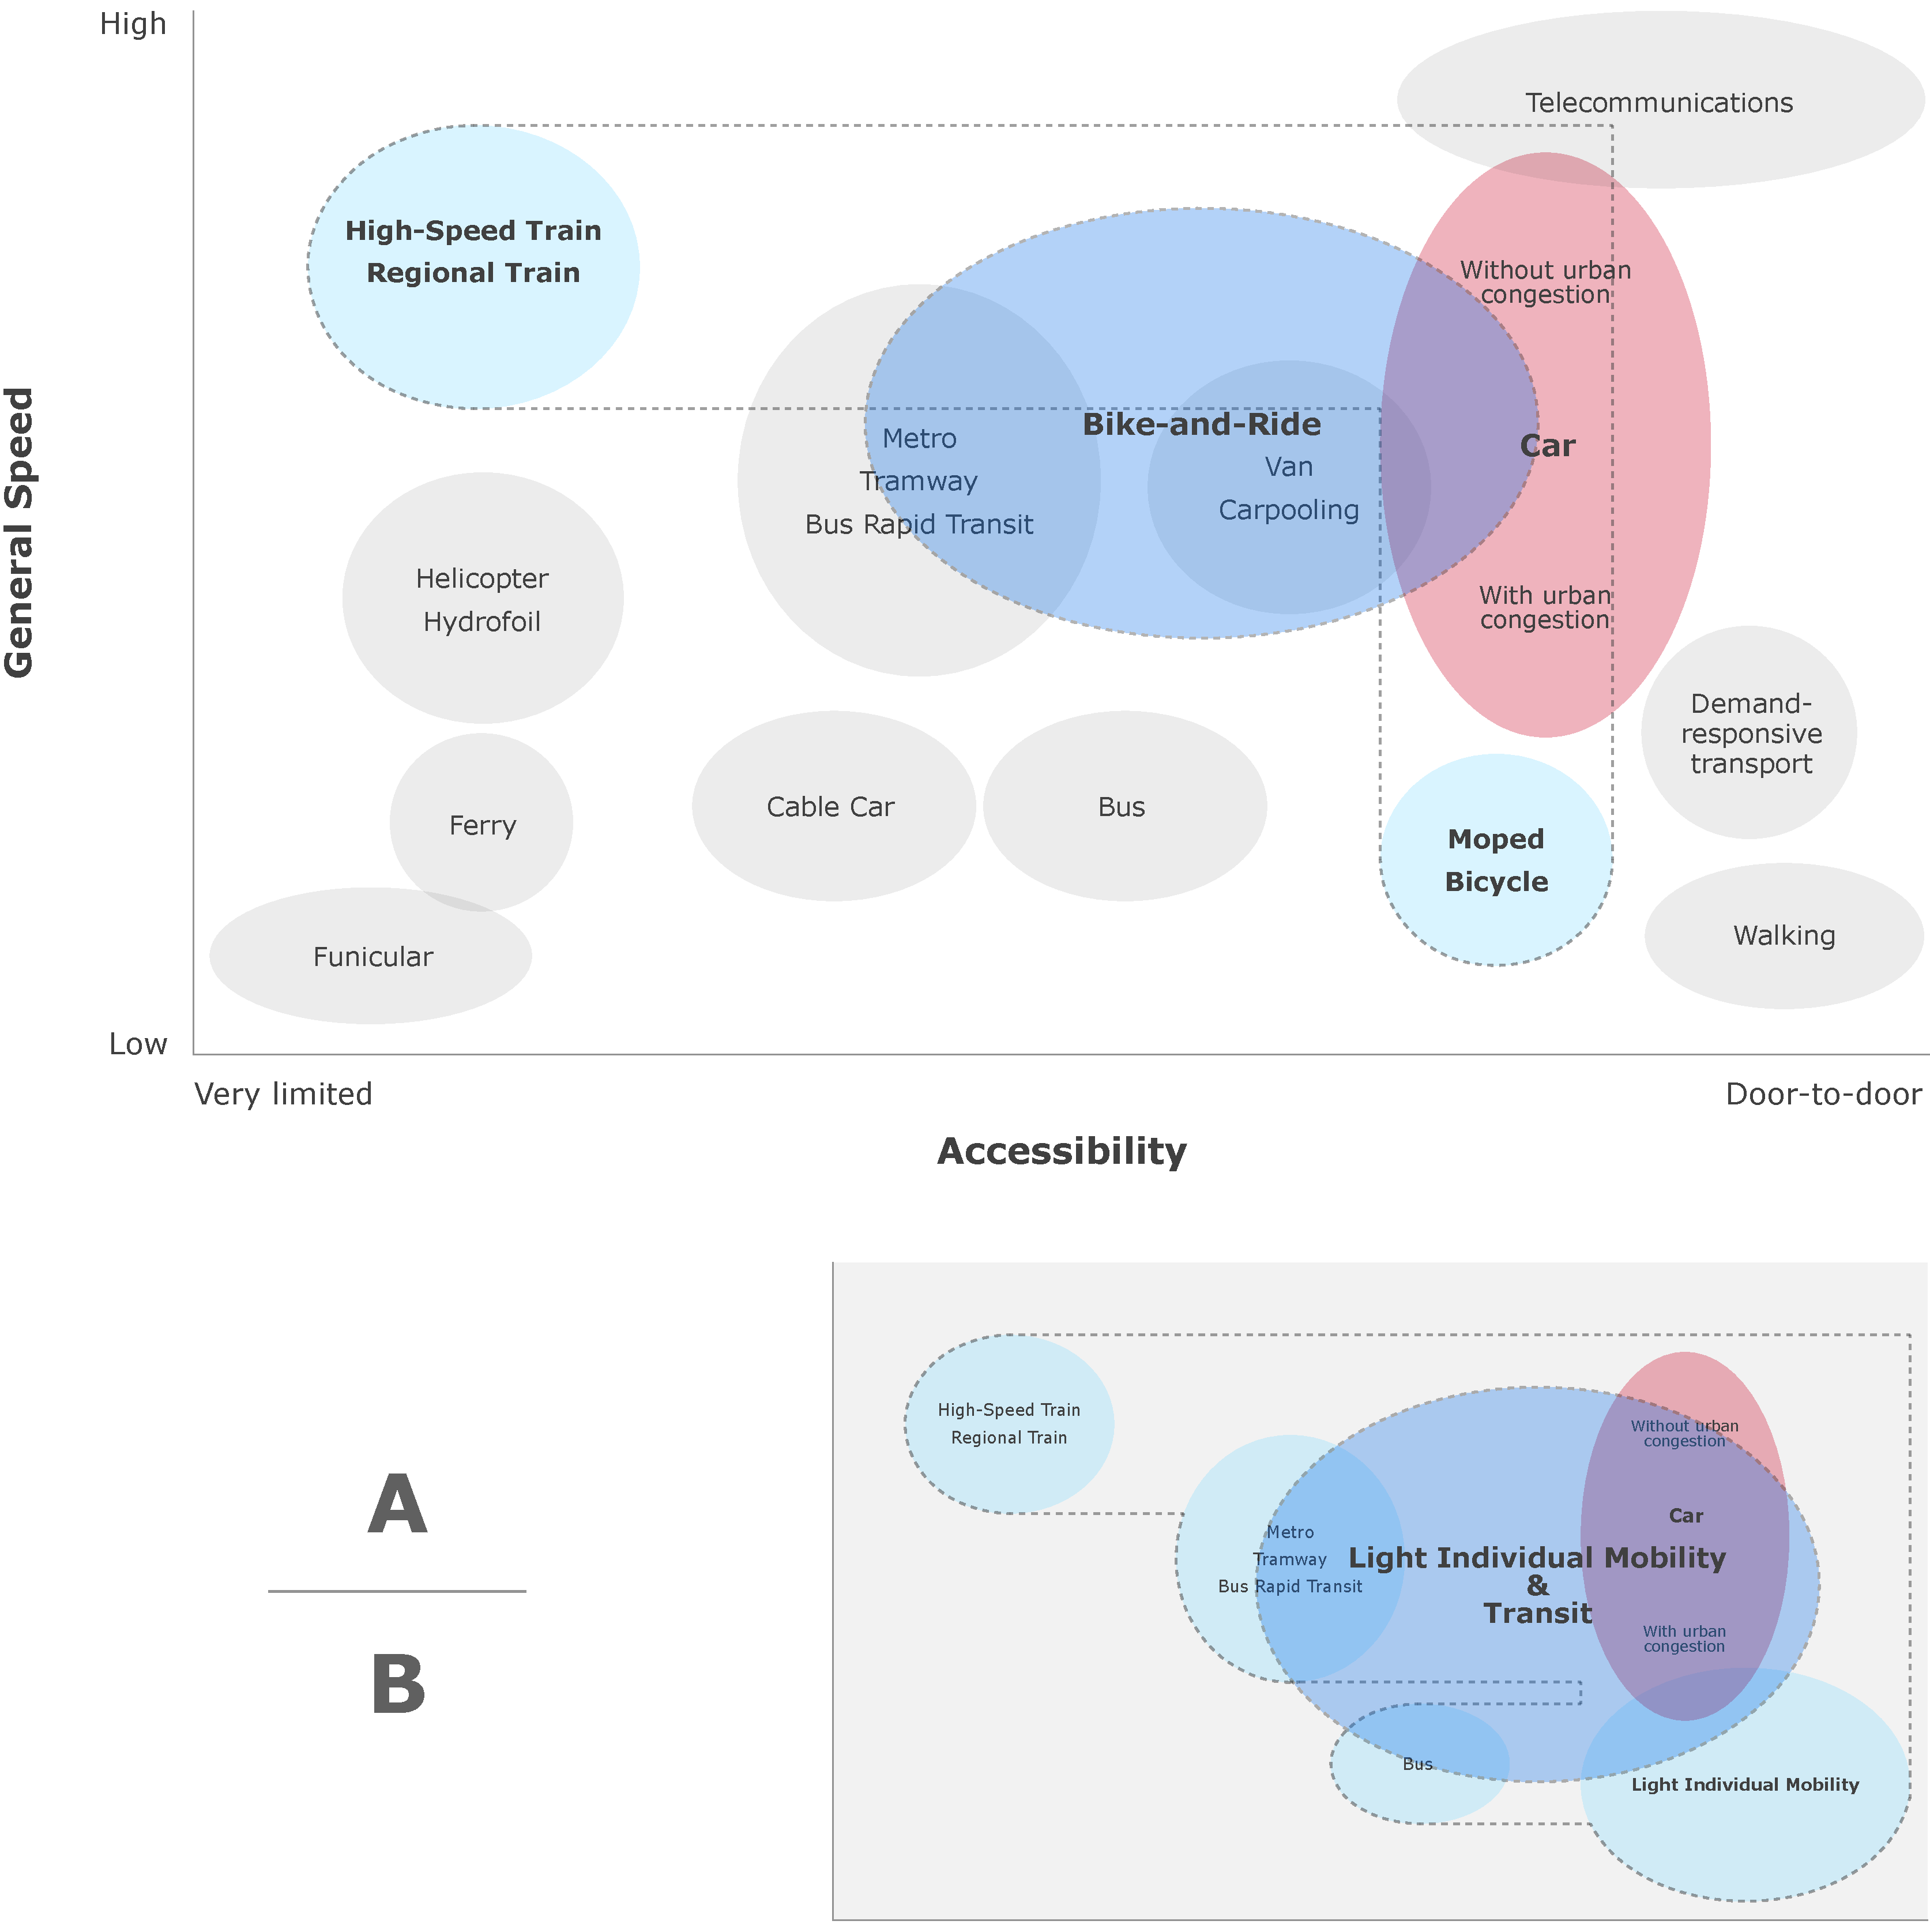
\includegraphics[width=1\columnwidth]{src/Figures/Chap-1/EN_Kager_vitesse_accessibilite.pdf}}
    \vspace{5pt}
    \begin{flushright}\scriptsize{
    Source (A): \textcolor{blue}{\textcite[212]{kager_characterisation_2016}}\index{Kager, Roland|pagebf}\index{Bertolini, Luca|pagebf}\index{te Brömmelstroet, Marco|pagebf}
    \\
    Graphic adaptation and reinterpretation (B): \textcolor{blue}{Dylan Moinse (2025)}
    }\end{flushright}
\end{figure}

% micromobility
While cycling is so well integrated into the \Commas{train system} in the Netherlands that a true bimodal mode of transport called \Commas{bike-train} has emerged \textcolor{blue}{\autocite[129-148]{bruntlett_curbing_2020}}\index{Bruntlett, Melissa|pagebf}\index{Bruntlett, Chris|pagebf}, \Commas{bike-train}, what about micromobility? It seems that this family of mobility devices serves a function and possesses properties similar to those of bicycles. Indeed, \acrshort{PMD}\textcolor{blue}{s} offer comparable potential for extending the reach of walking, allowing distances two to three times longer to be covered at a speed about three times higher \textcolor{blue}{\autocite{rabaud_micromobilites_2019}}\index{Rabaud, Mathieu|pagebf}\index{Richer, Cyprien|pagebf}. Thus, micromobility also contributes to redefining the catchment areas of public transport, facilitating access to stations and expanding their area of influence. A specific advantage of \acrshort{PMD}\textcolor{blue}{s}, however, lies in their compactness and lightness, which make them more easily carried on public transport, unlike traditional bicycles (see \hyperref[fig-chap1:vitesse-accessibilite-velo-tc]{Figure~\ref{fig-chap1:vitesse-accessibilite-velo-tc}}, page~\pageref{fig-chap1:vitesse-accessibilite-velo-tc}). Therefore, whether it’s a bicycle or micromobility devices, these modes meet similar needs and expectations: the pursuit of greater flexibility and direct, more flexible access to nodes that align with environmental goals \textcolor{blue}{\autocite[80]{oostendorp_combining_2018}}\index{Oostendorp, Rebekka|pagebf}\index{Gebhardt, Laura|pagebf}.%%Translated%%

% Impacts + Transition
The benefits of the combination of light individual mobility and public transport, including the increased distances that users are willing to travel to access or leave a public transport station, would contribute to a significant increase in the network's ridership \textcolor{blue}{\autocite[]{wang_approximating_2016}}\index{Wang, Hai|pagebf}\index{Odoni, Amedeo|pagebf}. A model developed by \textcolor{blue}{\textcite[69]{ensor_mode_2021}}\index{Ensor, Matt|pagebf}\index{Maxwell, O.|pagebf}\index{Bruce, Oliver|pagebf} shows that the rise of cycling and \acrshort{PeS} practices could lead to a 7\% increase in public transport ridership in urban areas, and a 9\% increase in suburban areas in New Zealand, if intermodal configurations are optimized. This finding highlights a key point: although cycling and micromobility cannot be fully competitive with the car over long distances and have limited capacity to replace it, their integration with public transport creates a synergy that makes them highly competitive against this mode of transport \textcolor{blue}{\autocite[43]{corporate_partnership_board_good_2020}}\index{Corporate Partnership Board@\textsl{Corporate Partnership Board}|pagebf}. As \textcolor{blue}{Annie-Claude} \textcolor{blue}{\textcite[262]{sebban_complementarite_2003}}\index{Sebban, Annie-Claude|pagebf}\index{Motte, Alain|pagebf} explains, the intermodality of cycling and public transport is structured around \textsl{practice territories}. This approach allows the concept of territory to be mobilized, as these intermodal practices operate \textsl{on} and \textsl{between} well-defined spaces. Considering intermodality from a territorial perspective naturally leads us back to the \acrshort{TOD} model. This framework appears to be a relevant one to revisit in light of the challenges related to the \Commas{first and last miles}, to which light individual mobility seems particularly suited.%%Translated%%

% 1.3.2.2.
\needspace{1\baselineskip} % Reserve space
\subsubsection*{Conceptualizing a Rail-Oriented Urbanism Supported by Light Individual Mobility
    \label{chap1:btod-m-tod}
    }

    % Introduction to secondary areas
In their work offering a contemporary view of \acrshort{TOD}, \foreignlanguage{english}{\textsl{Transit-Oriented Development and Sustainable Cities: Economics, Community and Methods}}, \textcolor{blue}{\textcite[222]{knowles_transit_2019}}\index{Knowles, Richard~D.|pagebf}\index{Ferbrache, Fiona|pagebf} emphasize the importance of leveraging opportunities provided by emerging mobilities in recent years—such as \acrshort{e-Bike}, \acrshort{PeS}, and dockless sharing services—in order to enrich the \acrshort{TOD} urban model. \textcolor{blue}{Peter} \textcolor{blue}{\textcite[54-55]{calthorpe_next_1993}}\index{Calthorpe, Peter|pagebf} does not disregard the importance of considering the \Commas{secondary areas} in the structuring of \acrshort{TOD} neighborhoods. He partially integrates them into \acrshort{TOD}, considering them sufficiently close to a public transport station to be oriented towards it, especially via a cycling connection. The \Commas{secondary area} even shares characteristics with the \Commas{primary area}, benefiting from some functional diversity and being connected to a network of calm streets. Far from being marginal, this area plays a structuring role in every train station district. It typically accommodates functions that are rarely configured to be placed in the most strategic area, such as jobs outside office spaces, schools, or parks. It also offers diversity in terms of housing choices, often including detached houses. The author identifies three types of \Commas{secondary areas}: (i) those separated by a road but close to a public transport stop; (ii) those separated by a road and distant from the stop; (iii) and those even farther from the stop but without a separating road \textcolor{blue}{\autocite[87]{calthorpe_next_1993}}\index{Calthorpe, Peter|pagebf}. Although the \Commas{secondary area} is often more car-oriented and frequently hosts infrastructure like \acrfull{PnR} encouraging the practice of park-and-ride, it should, according to him, be served by cycling connections directly linking it to the public transport station and the central train station district. From the moment \acrshort{TOD} is formalized, the major challenge lies in maximizing pedestrian and, especially, cycling connections within the \Commas{secondary area}. He specifically recommends the construction of separated bike lanes along major urban boulevards\footnote{~
    \Commas{\textsl{Due to the distances, bicycles are one of the most likely modes of travel for residents of secondary areas who are apt to use public transit. Strong bicycle connections following the shortest possible routes will provide additional encouragement for secondary area residents to use transit. Arterial roads and certain connecting routes in secondary areas must provide safe, separated or marked bicycle lanes allowing quick travel to the transit stop. Secondary area bicycle paths should connect to the TOD bicycle network.}} \textcolor{blue}{\autocite[89]{calthorpe_next_1993}}\index{Calthorpe, Peter|pagebf}.
} \textcolor{blue}{\autocite[60, 89]{calthorpe_next_1993}}\index{Calthorpe, Peter|pagebf}. In addition to these developments, the author emphasizes the importance of secure bike parking to encourage intermodal use, as well as the role of bicycles in internal mobility within the train station district\footnote{~
    \Commas{\textsl{Secure bike lockers are especially important for \Commas{bike-and-ride} transit use, as few will leave their bike unattended for a full working day. Bicycle parking facilities include bike racks, \Commas{checks,} and lockers. Bike racks must be provided at shopping, school, and recreational destinations in TODs and secondary areas. More secure bike parking facilities should be provided near all offices, workplaces, and major public transport stops.}} \textcolor{blue}{\autocite[103]{calthorpe_next_1993}}\index{Calthorpe, Peter|pagebf}.
} \textcolor{blue}{\autocite[103]{calthorpe_next_1993}}\index{Calthorpe, Peter|pagebf}. More than a simple connection to the main network, it is about offering a comprehensive cycling network that provides access to all amenities in the train station district—whether located in the primary or secondary area—and effectively linking one \acrshort{TOD} to another\footnote{~
    \Commas{\textsl{A coordinated system of bikeways should be provided in conjunction with TODs or a series of TODs. Important destinations, such as core commercial areas, transit stops, employment centers, parks, open spaces, schools, and other community facilities, should be linked by these bike routes.} [\dots] \textsl{Separated or marked bike lanes on several primary routes to the core area will support this alternative, as will the bike paths along greenways between TODs and employment destinations. On smaller streets, bikes sharing the travel lane will help slow cars to speeds more appropriate for residential streets. Selected routes to the transit stop should provide marked or separated bikeways connecting with the secondary areas and other key destinations. Designated bike lanes should be provided on selected connector streets and a limited number of local streets converging upon the commercial and transit center.} [\dots] \textsl{Clear destination signs should be provided that direct riders to key activity centers, such as shopping areas, transit stops, recreation facilities, schools, and bike parking facilities.}} \textcolor{blue}{\autocite[102]{calthorpe_next_1993}}\index{Calthorpe, Peter|pagebf}.
} \textcolor{blue}{\autocite[102]{calthorpe_next_1993}}\index{Calthorpe, Peter|pagebf}. Thus, considering the comparative advantages related to the integration of light individual mobility into the public transport network, the challenge goes beyond the simple \Commas{pedestrian pocket} to aim for a full integration of the \Commas{secondary area} within the \acrshort{TOD} \textcolor{blue}{\autocite[112]{ibraeva_transit-oriented_2020}}\index{Ibraeva, Anna|pagebf}\index{Almeida Correia, Gonçalo Homem de|pagebf}\index{Silva, Cecília|pagebf}.%%Translated%%

% Figure B-TOD
\begin{carte}[h!]\vspace*{4pt}
    \caption{Spatial configurations of the \textsl{Bicycle-based Transit-Oriented Development}.}
    \label{fig-chap1:schema-b-tod}
    \centerline{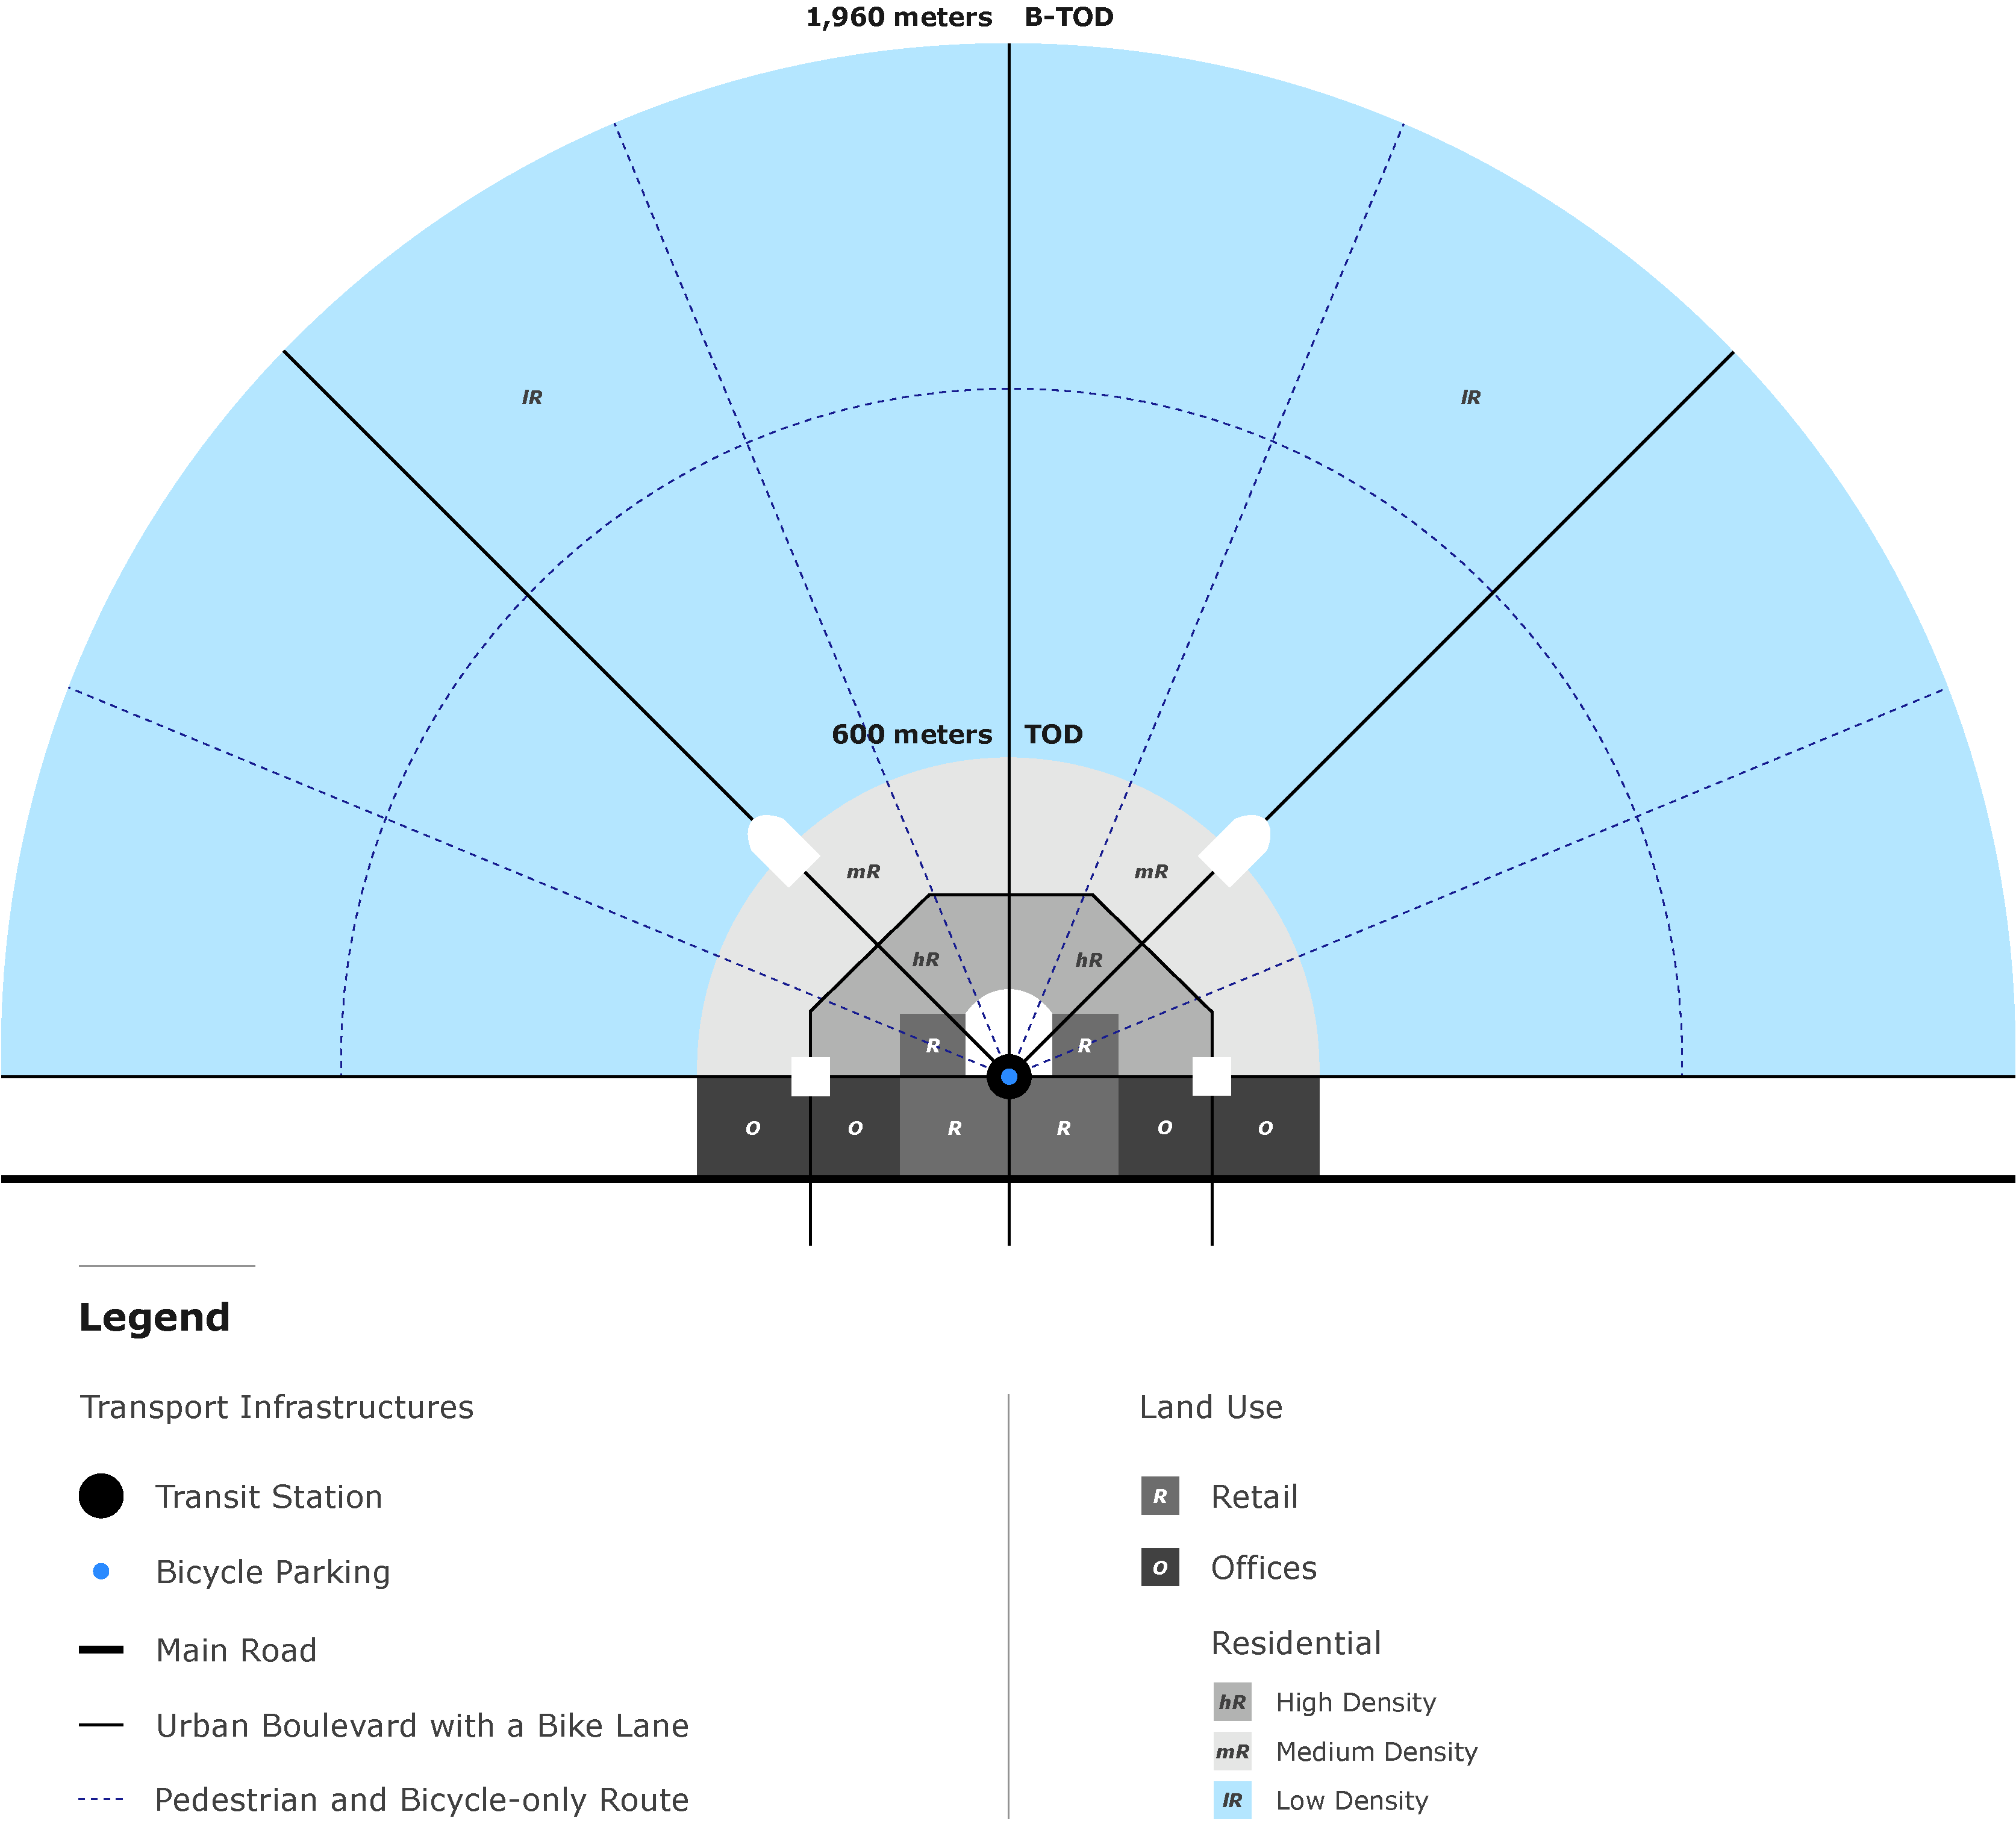
\includegraphics[width=1\columnwidth]{src/Figures/Chap-1/EN_Schema_B_TOD.pdf}}
    \vspace{5pt}
    \begin{flushright}\scriptsize{
    Source: \textcolor{blue}{\textcite[979]{lee_bicycle-based_2016}}\index{Lee, Jaeyeong|pagebf}\index{Choi, Keechoo|pagebf}\index{Leem, Yountaik|pagebf}
    \\
    Graphic adaptation: \textcolor{blue}{Dylan Moinse (2024)}
    }\end{flushright}
\end{carte}

% B-TOD
Although the issue of the \Commas{first and last miles} and the intermodal solution associated with cycling were considered as early as the foundational work of \acrshort{TOD}, it appears that the developments related to the \Commas{secondary area} and proposed cycling facilities have gradually lost visibility and clarity in the principles outlined. In response to this partial appropriation, South Korean researchers \textcolor{blue}{\textcite[979]{lee_bicycle-based_2016}}\index{Lee, Jaeyeong|pagebf}\index{Choi, Keechoo|pagebf}\index{Leem, Yountaik|pagebf}, in their article \textsl{Bicycle-based transit-oriented development as an alternative to overcome the criticisms of the conventional transit-oriented development}, propose, two decades later, the conceptualization of a \acrfull{B-TOD} (see \hyperref[fig-chap1:schema-b-tod]{Map~\ref{fig-chap1:schema-b-tod}}, page~\pageref{fig-chap1:schema-b-tod}). This variation of \acrshort{TOD}, which does not challenge the fundamental principles of the model, aims to address the needs of areas that have not reached the critical population and employment density thresholds necessary to maximize demand for transport around stations. The \acrshort{B-TOD} thus seeks to increase public transport network usage by targeting areas within a 2-kilometer radius accessible by bike \textcolor{blue}{\autocite[979]{lee_bicycle-based_2016}}\index{Lee, Jaeyeong|pagebf}\index{Choi, Keechoo|pagebf}\index{Leem, Yountaik|pagebf}. This revised model presents other notable advantages. It allows for an expansion of up to 25 times the area of a traditional train station district, thus significantly enhancing its attractiveness potential. Moreover, with easier implementation, it positions itself as an ecological alternative to the \acrshort{TOD} and \acrshort{E-TOD} models, requiring only a modest infrastructure investment \textcolor{blue}{\autocite[979, 983]{lee_bicycle-based_2016}}\index{Lee, Jaeyeong|pagebf}\index{Choi, Keechoo|pagebf}\index{Leem, Yountaik|pagebf}, as we discussed in the \hyperref[chap1:tod-presentation-generale-declinaisons-hybrids]{subsection on \textsl{Transit-Oriented Development} hybrids} (page~\pageref{chap1:tod-presentation-generale-declinaisons-hybrids}). A fourth advantage, less explicitly stated by the authors, is worth mentioning in our view: the \acrshort{B-TOD} could allow for an adaptation of the \Commas{[\dots] \textsl{population density criteria that would be more or less relaxed compared to those of the central area to maintain a more pleasant environment in this area.}}\footnote{~
    \Commas{\textsl{In a B-TOD setting, the re-establishment of the station impact area, where bicycle is a main access mode should be identified and the density criteria could be more or less relaxed than that of a TOD to keep the station impact area more pleasant.}} \textcolor{blue}{\autocite[983]{lee_bicycle-based_2016}}\index{Lee, Jaeyeong|pagebf}\index{Choi, Keechoo|pagebf}\index{Leem, Yountaik|pagebf}.
} \textcolor{blue}{\autocite[983]{lee_bicycle-based_2016}}\index{Lee, Jaeyeong|pagebf}\index{Choi, Keechoo|pagebf}\index{Leem, Yountaik|pagebf}. However, this does not mean reducing the density but rather better distributing it within the \acrshort{B-TOD} area by offering residential opportunities for individuals looking for less dense areas, better equipped with green spaces, offering easier access to family housing, or allowing escape from the land pressure surrounding centralities. To validate their conceptualization exercise, the authors conducted a survey with \Commas{intermodal cyclists}—this is the term we prefer to describe users combining cycling and public transport on the same trip—in the cities of Seoul and Daejeon. Their modeling shows that 94\% of the Seoul metropolitan area could be made accessible by public transport through intermodal cycling use, which is three times the coverage provided by combined walking \textcolor{blue}{\autocite[982]{lee_bicycle-based_2016}}\index{Lee, Jaeyeong|pagebf}\index{Choi, Keechoo|pagebf}\index{Leem, Yountaik|pagebf}. Reorganizing urbanism around public transport and bicycles not only promotes ecology but also health and physical activity \textcolor{blue}{\autocite[44]{heran_velo_2020}}\index{Héran, Frédéric|pagebf}\index{Rymarski, Christophe|pagebf}\index{Bedin, Véronique|pagebf}, a dimension less addressed in conventional \acrshort{TOD}.%%Translated%%

% M-TOD
Building on this variation, we have chosen to rely on this foundational research work, which seems to be the cornerstone, in order to draw inspiration from it and transpose our argument developed throughout this chapter. Specifically, it aims to demonstrate the potential of light individual mobility to strengthen the urban model of \acrshort{TOD}, with a view to promoting more sustainable mobility and urban environments. Drawing inspiration from the arguments put forward by \textcolor{blue}{\textcite{lee_bicycle-based_2016}}\index{Lee, Jaeyeong|pagebf}\index{Choi, Keechoo|pagebf}\index{Leem, Yountaik|pagebf}, and particularly revisiting their questions regarding the \Commas{identification} and \Commas{definition} of a \acrshort{B-TOD}, we propose an update of these models to design an \acrfull{M-TOD}. Ultimately, we could transpose the proposal for a \Commas{general theory of walkability} formulated by urban planner \textcolor{blue}{Jeff} \textcolor{blue}{\textcite[73]{speck_walkable_2013}}\index{Speck, Jeff|pagebf} into a \Commas{general theory of bikeability} articulated around the public transport system. This would integrate all light individual mobility and fulfill, just like walkability, a threefold function: that of a purpose in itself, a means of accessibility, and a measure of urban quality \textcolor{blue}{\autocite[73]{speck_walkable_2013}}\index{Speck, Jeff|pagebf}. Thus, several questions structure, at this stage, our reflection:
\begin{customitemize}
\item What is an \acrshort{M-TOD} and how does it differ from a \acrshort{TOD} and a \acrshort{B-TOD}?
\item What are its observable uses and what is its modal shift potential?
\item What are the connections between public transport and light individual mobility?
\item How do these current and potential mobility behaviors interact with the urban fabric and territorial development challenges?
\end{customitemize}%%Translated%%

% ___________________________________________
% 1.*.
\newpage
\needspace{1\baselineskip} % Reserve space
\addcontentsline{toc}{section}{Conclusion of Chapter~1}
\sectionheader{Conclusion of Chapter~1}
\section*{Conclusion of Chapter~1
    \label{chap1:conclusion}
    }
    \markright{Conclusion of Chapter~1}{}

    % Introduction
The \acrfull{TOD} now constitutes a strategic lever for sustainable urban planning, offering a response to the challenges posed by the \Commas{car everywhere} and \Commas{car above all} policies, which continue to guide urban development in France \textcolor{blue}{\autocite[14]{sebban_complementarite_2003}}\index{Sebban, Annie-Claude|pagebf}\index{Motte, Alain|pagebf}. This chapter has revisited the historical foundations, guiding principles, and contemporary variations of this urban planning model. Although its formalization emerged in the North American context, it would be wrong to attribute its creation exclusively to American urban planners, as they themselves acknowledged drawing inspiration from European examples \textcolor{blue}{\autocite[15]{renne_emerging_2004}}\index{Renne, John Luciano|pagebf}\index{Wells, J.~S.|pagebf}. In sum, the theoretical and operational framework of \acrshort{TOD} provides a solid and relevant foundation for addressing current environmental and socio-economic imperatives, both at the regional and local levels. It is not only about promoting a better public transport offer—although this is a necessary condition—but about integrating this offer within an interaction with territorial structuring \textcolor{blue}{\autocite[9]{bernier_atlas_2023}}\index{Bernier, Xavier|pagebf}, following a dynamic of \Commas{congruence}\footnote{~
    In his article titled \textsl{The \Commas{structural effects} of transport: political myth, scientific mystification}, \textcolor{blue}{Jean-Marc} \textcolor{blue}{\textcite[239]{offner__1993}}\index{Offner, Jean-Marc|pagebf} notably exposed the need for a \Commas{demystification} of the political-media and scientific discourse concerning the evaluation and expectations surrounding the \Commas{structural effects} of transport infrastructure. He challenges the idea of a linear causal relationship between the introduction of new mobility offerings and territorial development, highlighting a more complex pre-existing dynamic of parallel connections, which he terms \Commas{congruence}.
}, a concept developed by \textcolor{blue}{Jean-Marc} \textcolor{blue}{\textcite[239]{offner__1993}}\index{Offner, Jean-Marc|pagebf}. The goal of \acrshort{TOD} is therefore not so much to \Commas{generate growth} (economic, demographic, or urban) in absolute terms, but rather to redistribute it more evenly within a given region \textcolor{blue}{\autocite[82]{cervero_transit_1998}}\index{Cervero, Robert|pagebf}.%%Translated%%

% Forces du TOD
The main benefit of \acrshort{TOD} neighborhoods \textcolor{blue}{\autocite[40]{bentayou_transit-oriented_2015}}\index{Bentayou, Gilles|pagebf} lies not only in their ability to attract new riders to public transport, but also in their capacity to create pleasant urban environments characterized by density and livability. Ultimately, this urban planning strategy fully aligns with the third prospective scenario studied by SNCF\footnote{~
    The study commissioned by SNCF explores the possible future mobility trends in France by 2050, along with their environmental and social implications. Building on the reflections of French and international experts, it also incorporates results from a survey conducted by \acrfull{IFOP} in 2015 with 1,800 French participants. Three prospective scenarios are outlined based on the dynamics of mobility demand and transport supply: (i) \Commas{ultramobility: faster, further}; (ii) \Commas{altermobility: moving differently}; and (iii) \Commas{proximobility: the quality of proximity} which incorporates \Commas{altermobility}. Among these scenarios, only the last one would allow the national objective of reducing \acrfull{GHG} emissions by a factor of four (\textsl{Factor 4}), while generating an annual savings of~\euro~100 billion for society compared to the current situation and the other two trajectories considered \textcolor{blue}{\autocite[26-37]{sncf_vers_2015}}.
}, the \Commas{proximobility} scenario, which is based on the establishment of an alternative mobility system to the car (\Commas{altermobility}) in line with a territorial reconfiguration favoring better local anchoring, the development of active modes, and urban densification \textcolor{blue}{\autocite[26-37]{sncf_vers_2015}}\index{SNCF@\textsl{SNCF}|pagebf}. This scenario is actually the only one capable of achieving the goal of reducing \acrfull{GHG} emissions by a factor of four by 2050, while ensuring effective coordination between the transport system, urban organization, and micro-circulations within train station neighborhoods \textcolor{blue}{\autocite[148]{krakovitch_metropolitrain_2019}}\index{Krakovitch, Alain|pagebf}. In other words, only a comprehensive overhaul of territorial organization will allow us to \Commas{tear the car out of the city} \textcolor{blue}{\autocite[184]{ducharme_ville_2021}}\index{Ducharme, Olivier|pagebf}.%%Translated%%

% Micro-mobilité
The integration of light individual mobility within the framework of \acrshort{TOD} supports a position that complements the public transport network, enhancing the overall efficiency of the alternative mobility system and contributing to the emergence of an \Commas{energy sobriety} or a \Commas{post-carbon city} \textcolor{blue}{\autocite[2]{schultz_micromobility_2019}}\index{Schultz, Stéphane|pagebf}\index{Grisot, Sylvain|pagebf}. Driven by the rise of new forms of travel, electromobility, and the development of shared services, with or without docking stations, light individual mobility addresses emerging needs that go beyond the traditional dichotomy between personal vehicles and public transport. It has become a practical and flexible solution, enabling users to become true \Commas{augmented pedestrians} \textcolor{blue}{\autocite[1]{boffi_extrait_2019}}\index{Boffi, Nicolas|pagebf}. As stated by the Secretary-General of the \acrfull{UITP}, light individual mobility \Commas{ [\dots] \textsl{is an integral part of public transport because it meets objectives that are also converging, namely: better use of urban space, reduced emissions of pollutants and greenhouse gases; moreover} [\dots] [it] \textsl{can be easily combined with traditional public transport~–~both physically and in terms of services and fares} [\dots]} \footnote{~
    \Commas{[\dots] \foreignlanguage{english}{\textsl{micromobility is an integral part of public transport because it meets objectives that are also converging, namely: better use of urban space, less emissions of pollutants and greenhouse gases; plus micromobility modes can be easily combined with traditional public transport~–~both physically and in terms of services and fares}} [\dots]} \textcolor{blue}{\autocite{bcg_role_2020}}.
} \textcolor{blue}{\autocite{bcg_role_2020}}\index{BCG@\textsl{BCG}|pagebf}. It is important to recall that \acrshort{TOD} remains a flexible model, whose application varies according to specific contexts and issues. Its guiding principles do not constitute a rigid framework, but rather an \textsl{ethos}, as \textcolor{blue}{Peter} \textcolor{blue}{\textcite[11]{calthorpe_next_1993}}\index{Calthorpe, Peter|pagebf} points out. In this sense, we have observed that \textsl{Transit Metropolises} have evolved over recent decades by integrating hybrid approaches, combining interventions on both the supply and demand for mobility \textcolor{blue}{\autocite[137-143]{cervero_transit_2020}}\index{Cervero, Robert|pagebf}.%%Translated%%

% B-TOD
Beyond the simple development of \Commas{smart vehicles}, light individual mobility establishes itself as a key player that first optimizes the \Commas{intelligence of flows, space, and networks} into which these vehicles are integrated \textcolor{blue}{\autocite[76]{krakovitch_metropolitrain_2019}}\index{Krakovitch, Alain|pagebf}. Its potential is particularly revealed in the modal chain of travel, where it enhances the effectiveness of public transport while offering a fluid and adaptable alternative to mobility needs \textcolor{blue}{\autocite[4]{molino_pratiques_2015}}\index{Molino, Marie|pagebf}\index{Rampon, Anne-Sophie|pagebf}\index{Cipolla, Romain|pagebf}. This \Commas{hybrid} model, both efficient, flexible, and competitive compared to the car \textcolor{blue}{\autocite[107]{wang_bicycle-transit_2013}}\index{Wang, Rui|pagebf}\index{Liu, Chen|pagebf}, avoids the pitfall of expanding the deployment margins of the automobile system, unlike the risks posed by autonomous cars. Instead, it proposes a diversified \Commas{bouquet of offers} that breaks the \Commas{car reflex} and promotes a transition towards more sustainable mobility \textcolor{blue}{\autocites[81]{bertolini_planning_2017}[42]{6t-bureau_de_recherche_livre_2019}}\index{Bertolini, Luca|pagebf}\index{Bureau de recherche 6t@\textsl{Bureau de recherche 6t}|pagebf}. \textcolor{blue}{Annie-Claude} \textcolor{blue}{\textcite[35]{sebban_complementarite_2003}}\index{Sebban, Annie-Claude|pagebf}\index{Motte, Alain|pagebf} presents it as follows: \Commas{\textsl{Instead of asking whether the complementarity between bike and public transport is detrimental to public transport vehicle flow, shouldn't the question be framed as: is the complementarity between bike and public transport a practice, or even a policy, sufficiently detrimental to car traffic?}} In this perspective, \textcolor{blue}{Georges} \textcolor{blue}{\textcite[225]{amar_homo_2016}}\index{Amar, Georges|pagebf} emphasizes the need to create bridges and synergies between new forms of mobility and emerging urban models. Contemporary cities must therefore promote this \Commas{reliance}, an approach also developed by \textcolor{blue}{\textcite[979]{lee_bicycle-based_2016}}\index{Lee, Jaeyeong|pagebf}\index{Choi, Keechoo|pagebf}\index{Leem, Yountaik|pagebf} through their conceptualization of a \acrfull{B-TOD}.%%Translated%%

% Figure Google scholar trends
\begin{figure}[h!]\vspace*{4pt}
    \caption{Number of international scientific publications on \textsl{Transit-Oriented Development}, micromobility, or their combination.}
    \label{fig-chap1:trends-google-scholar}
    \centerline{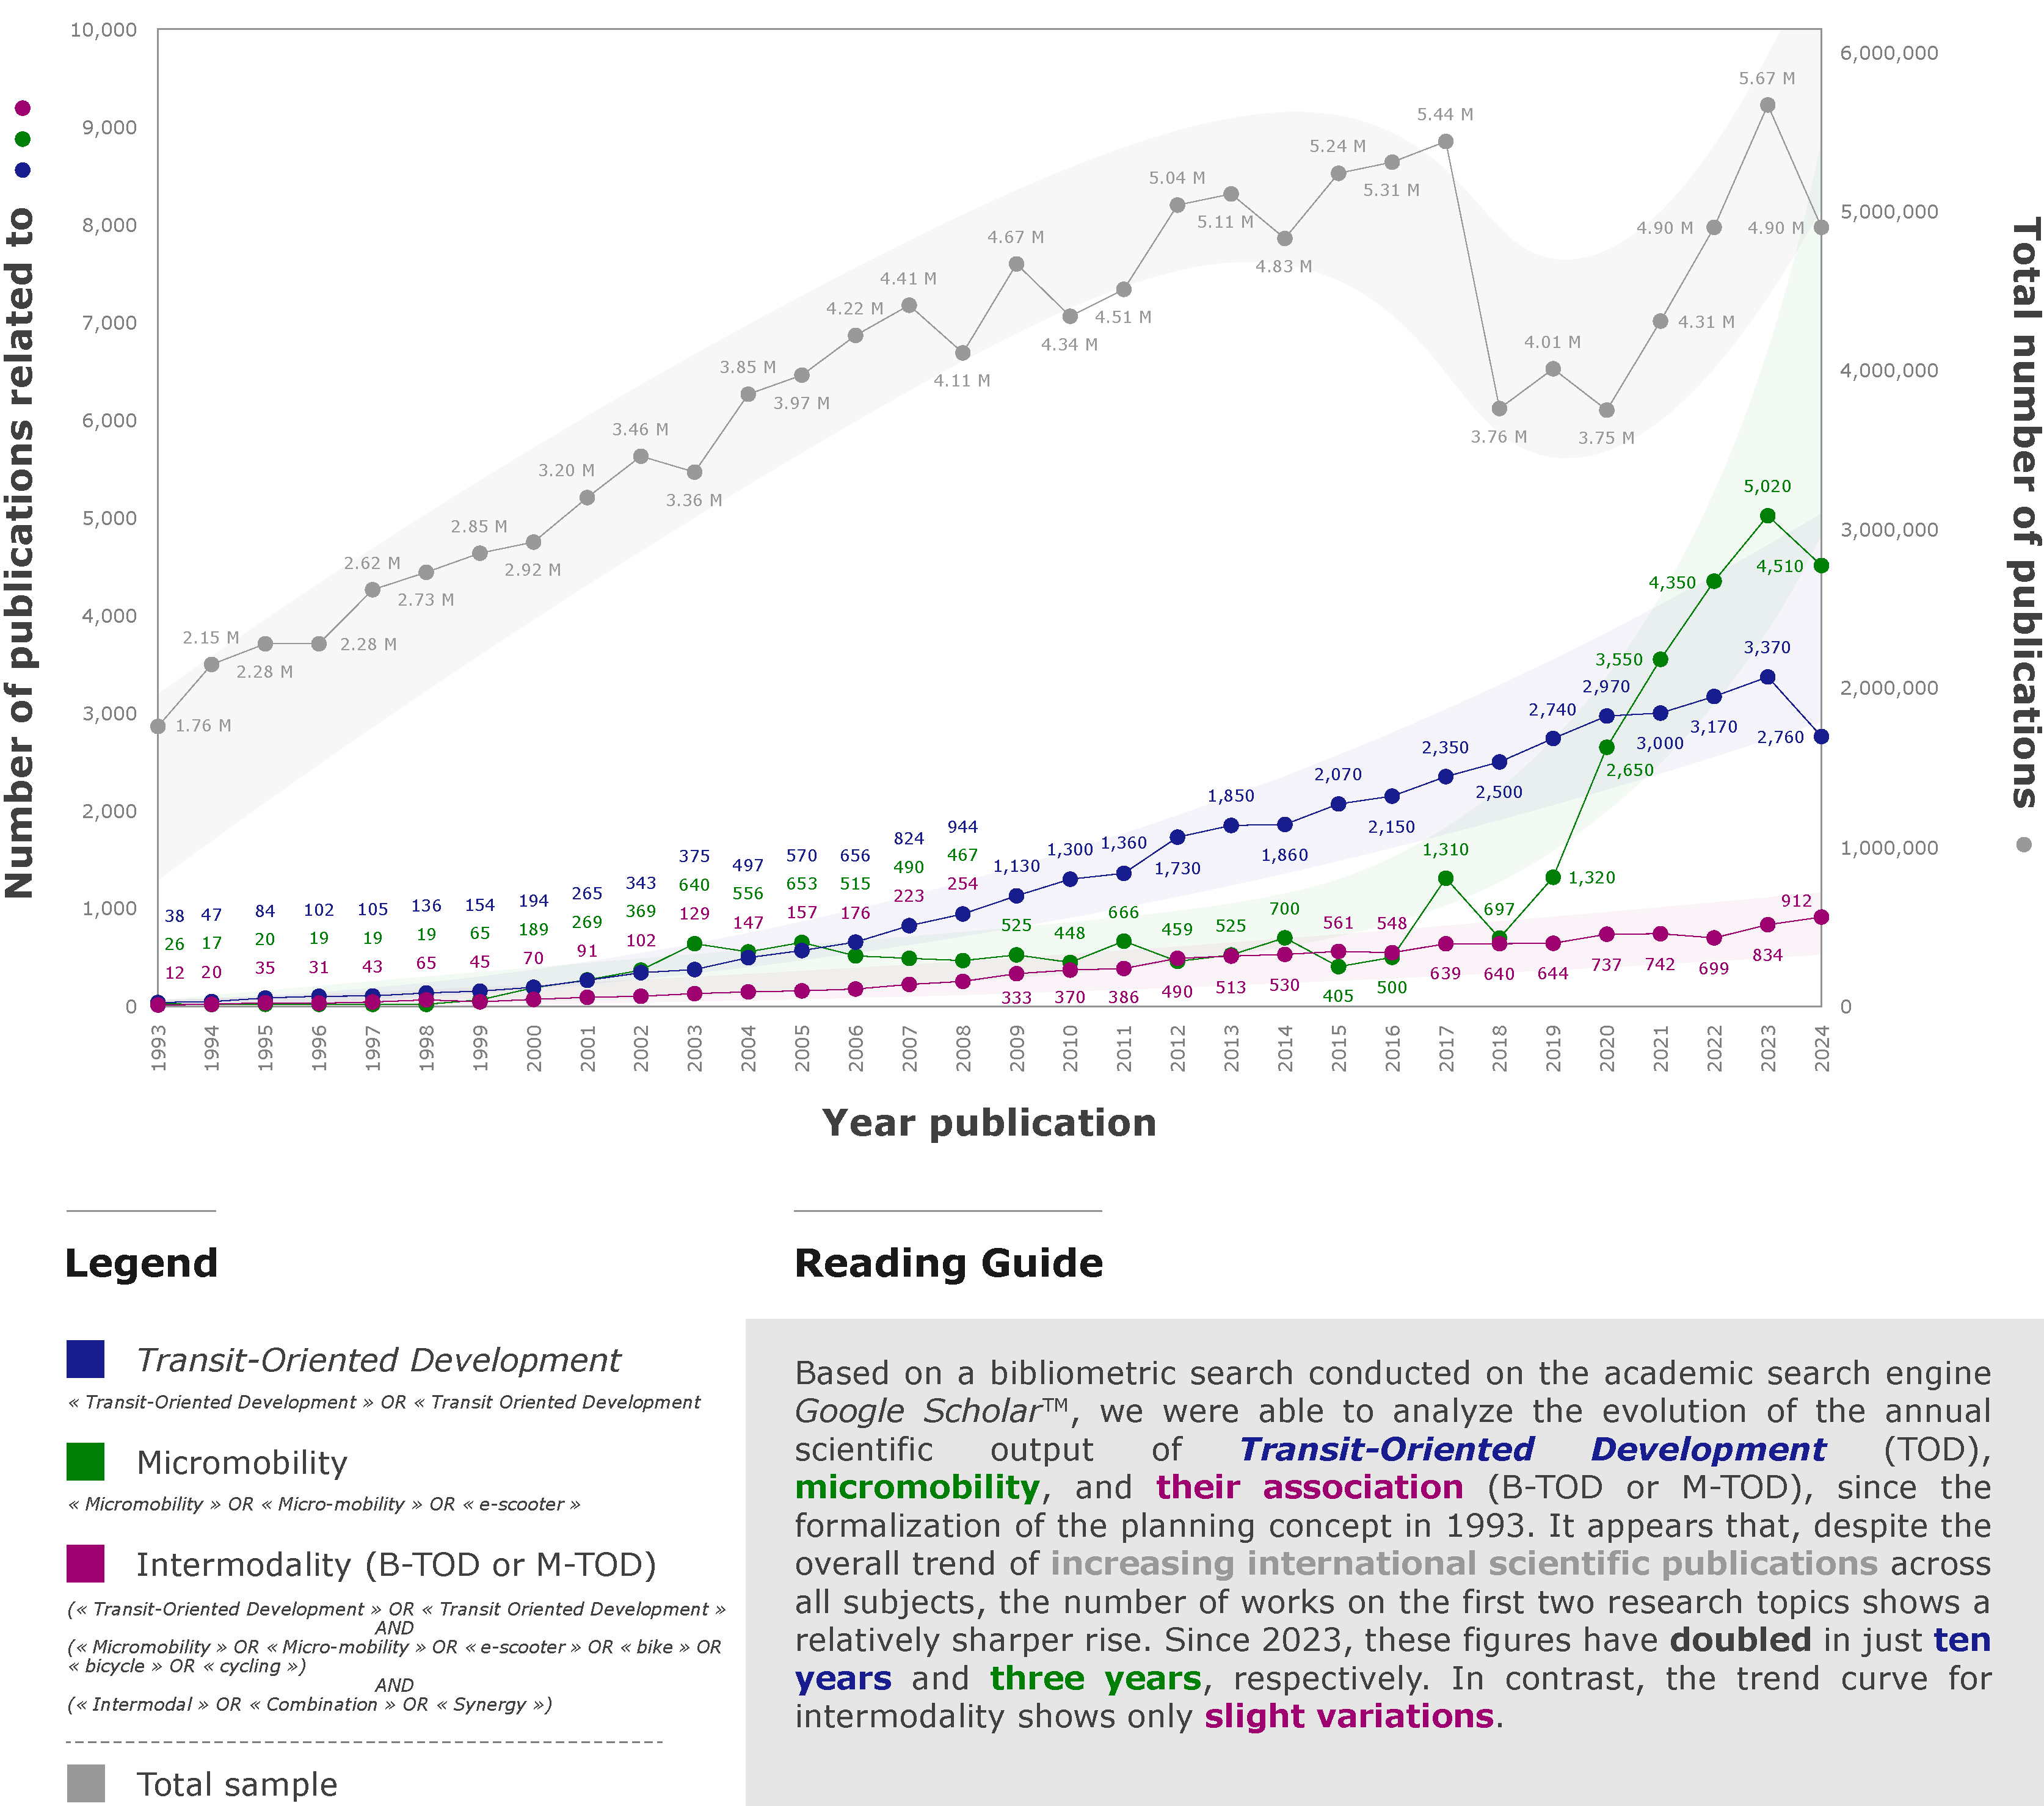
\includegraphics[width=1\columnwidth]{src/Figures/Chap-1/EN_Chronologie_publications_TOD_MIL.pdf}}
    \vspace{5pt}
    \begin{flushright}\scriptsize{
    Source: bibliometric data from \Marque{Google Scholar} exported on February 2, 2025
    \\
    Author: \textcolor{blue}{Dylan Moinse (2025)}
    }\end{flushright}
\end{figure}

% M-TOD + Transition
One of the recent developments in \acrshort{TOD} explored in this chapter concerns the integration of light individual mobility. These modes of transportation complement traditional infrastructures by providing effective solutions to the challenges of the \Commas{first and last miles}. However, knowledge of this form of intermodality, particularly in its interaction with urban forms, remains limited. This is especially true for emerging mobilities that make up this family of modes, whose interactions with \acrshort{TOD} remain largely unexplored. A simple lexical search on the themes of \acrshort{TOD} and micromobility illustrates how these topics are gaining increasing interest in academic research, as shown in \hyperref[fig-chap1:trends-google-scholar]{Figure~\ref{fig-chap1:trends-google-scholar}} (page~\pageref{fig-chap1:trends-google-scholar}). Nevertheless, this growing interest has not yet translated into a true synergy between these two fields of study, which remain underrepresented together in the scientific literature. This chapter, which sets the theoretical framework for our research, thus concludes with the observation of a knowledge gap \textsl{a priori} on a topic recently rediscovered in the context of \acrshort{TOD}. This gap is also highlighted by \textcolor{blue}{Wei} \textcolor{blue}{\textcite[90]{kang_university_2020}}\index{Kang, Wei|pagebf}\index{Aguiléra, Anne|pagebf}\index{Rallet, Alain|pagebf}, who points out in his doctoral thesis the low number of studies dedicated to intermodality between new mobility services, such as the \acrshort{DBS}, and public transport. Similarly, \acrshort{PeS} and \acrshort{DESS} have been marginally studied, beyond issues related to trauma or accidentology, even though their intermodal potential is widely reported \textcolor{blue}{\autocite{richer_dossier_2021}}\index{Richer, Cyprien|pagebf}. Conducting rigorous empirical studies on these forms of intermodality appears to be a requirement to measure and understand behaviors related to \textsl{bike-and-ride} and \textsl{scoot-and-ride} \textcolor{blue}{\autocite[13]{bortoli_consequential_2020}}\index{Bortoli, Anne de|pagebf}\index{Christoforou, Zoi|pagebf}. Given this assessment, we have chosen to initiate an exploratory study on what we call \acrshort{M-TOD}, by compiling existing works on this topic, which will be presented in the next chapter.%%Translated%%

% ___________________________________________
     \newpage
     
% Valorisation scientifique
    \begin{tcolorbox}[colback=white!5!white,
                      colframe=blue!75!blue,
                      title=Valorization
                      \\
                      Chapitre~1]
\Large{\textcolor{blue}{\textbf{Seminars:}}}
    \\\\
\small{\textcolor{blue}{\textcite{moinse_transit-oriented_2021}}. Le Transit-Oriented Development, un urbanisme axé sur les transports en commun, intégrant les micro-mobilités émergentes. Une investigation sur les trottinettes personnelles en intermodalité, dans la région Hauts-de-France. \textsl{Rencontres TerriTrans - MoTAU}, Paris.
\\
\footnotesize{\url{https://hal.science/hal-03473391}} (\textbf{C-COM})}
    \\\\
\small{\textcolor{blue}{\textcite{moinse_modeurbain_2021}}. Le modèle urbain du Transit-Oriented Development revisité par les mobilités émergentes? Une investigation sur le territoire de la région Hauts-de-France. \textsl{Rencontres Internationales en Urbanisme de l'APERAU}, Rabat.
\\
\footnotesize{\url{https://shs.hal.science/halshs-03507291}} (\textbf{C-COM})}
    \\\\
\small{\textcolor{blue}{\textcite{moinse_modeurbain_2020}}. Le modèle urbain du Transit-Oriented Development revisité par les micro-mobilités émergentes? Une investigation sur le territoire de la région Hauts-de-France. \textsl{(Post-)Doctoriales AME 2020}, Le Croisic.
\\
\footnotesize{\url{https://shs.hal.science/halshs-03507482}} (\textbf{C-COM})}
    \\\\
\small{\textcolor{blue}{\textcite{moinse_etat_2020}}. État de l'art sur l'usage des trottinettes électriques en libre-service sans station. \textsl{Journées Transports \& Déplacements du Réseau Scientifique et Technique} (JTD RST). 
\\
\footnotesize{\url{https://shs.hal.science/halshs-03507375}} (\textbf{C-COM})}
    \\\\
\Large{\textcolor{blue}{\textbf{Communication:}}}
    \\\\
\normalsize{\textcolor{blue}{\textcite{moinse_exploring_2023}}. \foreignlanguage{english}{\textsl{Exploring Val d'Europe's Urban Development in Marne-la-Vallée: A Guided Walking Tour of the TOD Project}}, Présentation de terrain, Paris
\\
\footnotesize{\url{https://shs.hal.science/halshs-04212064}}}
    \end{tcolorbox}

    % ___________________________________________
    % Subbibliography
    \newpage
    \sectionheader{Bibliography of Chapter~1}
    \begingroup
    \renewcommand{\bibfont}{\scriptsize}
\printbibliography[segment=\therefsegment, heading=subbibintoc, title={Bibliography of Chapter~1}, label=chap1:bibliographie]
    \endgroup
    \end{refsegment}